% -*- root: These.tex -*-

\newcommand\litem[1]{\item{\bfseries #1,\enspace}}

\section{Une plateforme \textit{High Performance Computing} (HPC) pour l'exploration de modèle de simulation en géographie : OpenMOLE}
\label{sec:retourgeoHPCopenmole}

\epigraph {Fou de joie, le géographe s'appuya de tout son long sur le clavier pour en enfoncer toutes les touches; et de la multitude des composants, circuits, transistors, condensateurs et rupteurs, des disques et des disquettes, des fils et des interfaces, des périphériques, sphériques et féériques, des matériels, des logiciels, des progiciels et de près du Ciel, monta une prodigieuse clameur.

C'était le chant du monde.

Alors le géographe s'endormit, apaisé, car il était comblé.}{ --- \textup{Henry Chamussy - Songe d'une nuit de calcul.. - 1984}}

\epigraph {I know I've made some very poor decisions recently, but I can give you my complete assurance that my work will be back to normal. I've still got the greatest enthusiasm and confidence in the mission. And I want to help you.}{ --- \textup{HAL9000 - 2001, l'odysée de l'espace  - 1968}}

\subsection{Engager \enquote{un retour} vers le HPC en géographie}
\label{ssec:retourHPC}

Si le terme de \textit{High Performance Computing} HPC semble d'origine récente lorsqu'il est entrepris par les institutions \autocite{HPCHorizon2020}, il suffit d'oser jeter un regard en arrière pour trouver l'emploi du terme chez les géographes à la fin des années 1990. A la lecture de ces ouvrages \autocites{Turton1998, Openshaw2000, Openshaw2000b}, on s'aperçoit que cet acronyme n'a vraiment de sens que si on le contextualise. Ainsi, pour \textcite{Openshaw2000} \foreignquote{english}{The term \enquote{HPC} is very easy: it stands for high-performance computing (or \enquote{computer} depending on context), but the definition of what is \enquote{high-performance} is vague, relative and almost constantly changing as hardware continues to improve. It is a characteristic feature that today's workstations now offer levels of performance (or better) than only three-five years ago required extremely expensive HPC hardware in the form of vector supercomputers.}

En ce sens, la source brute de calcul impliquée par le terme HPC sous sa forme actuelle correspondra probablement d'ici 20 ans à la puissance d'un micro-ordinateur standard, comme on déjà pu le voir dans le passé sous le coup de la loi de Moore, dont on a fêté il y a peu les 50 ans (1965 - 2015); une loi quasiment devenue pour certains observateurs une prophétie autoréalisatrice, de par la pression économique et la course à l'innovation qu'elle maintient dans l'industrie et la recherche. Qui plus est, créer et utiliser de super-ordinateurs (\textit{supercomputers}) pour réaliser des prouesses en calculs impossible autrement, et cela avec ou sans parallélisme des applications, cette idée trouve comme on le verra plus loin des racines évidentes dans les tout débuts de l'informatique.

Le HPC ne peut donc que difficilement être vanté comme provenant d'une quelconque révolution matérielle ou logicielle récente, et ne se substitue qu'à l'expression logique d'un mouvement entamé il y a bien longtemps, celui-ci s'étant largement diversifié par la suite. Se sont ainsi succédé depuis les années 1930 (Z1 mécanique) / 1950 (ENIAC électronique), une longue série d'innovations dans le matériel, le logiciel, et plus généralement dans les paradigmes informatiques qui peuvent les motiver. Le HPC est donc un terme utilisé pour pointer tout autant les anciens (le mythique et monstrueux Cray-1 de 1976) que les plus récents super-ordinateurs (ADA ou TURING du laboratoire CNRS IDRIS, 230 et 1258 TFlops), mais également depuis les années 1990 la mise en réseau local d'ordinateurs standards à moindre coût \Anote{projet_beowulf}, ou encore une puissance répartie sur la base d'une mise en réseau de cartes micro-pc \Anote{projet_parallela}, ou de milliers d'ordinateurs de particuliers bénévoles (le 13 mai 2015 l'initiative BOINC rassemble 720000 ordinateurs et totalise 6,7 PFlops \Anote{puissance_collective}); sans compter enfin cette infrastructure scientifique nommée grille de calcul supportant à une maille locale, nationale, ou internationale la mise en réseau de tout ce qu'il convient d'appeler aujourd'hui de façon générique des noeuds de calculs tant leur nature est hétérogène.

Il y a évidemment des différences dans l'organisation et la gestion de ces différentes ressources, ou les motivations guidant leur construction et leur bonne utilisation; mais en soi, la finalité du projet semble assez similaire, avec la mise à disposition au plus grand nombre d'une ressource de calcul permettant la résolution la plus rapide possible, et/ou à moindre coût, de problèmes scientifiques ou industriels de nature plus ou moins complexe.

Le terme HPC ne semble être au final qu'une réminiscence d'une course à la performance d'origine bien plus ancienne; un terme parapluie qui accueille dans son ombre une diversité toujours plus grande de matériels et de logiciels.

L'\textit{European Technology Platform for HPC} (ETP4HPC) créé en 2011, reconnu comme la plateforme de référence pour l'établissement de partenariat public privé et la réalisation des objectifs du projet HPC de l'Horizon2020 \autocite{ETP4HPC2013}, définit le HPC ainsi :

\foreignquote{english}{
High-Performance Computing (HPC) refers to any form of computing where the density of processing or the size of the problems addressed require more than a standard or commodity computing system in order to achieve the expected result under the given constraints, and the application of advanced techniques such as the use of multiple processors (tens, hundreds, thousands or even more) connected together by some kind of network to achieve a performance well above that of a single processor. Both projects began in 1993, with significant systems deployed in 1994, and both had strong
impact on the community, essentially defining the range
of capabilities and techniques to be incorporated to this
day.

Two traditional HPC categories are distinguished:

\begin{itemize}
\item Capability computing refers to the use of a large and high-performing computing infrastructure to solve a single, highly complex problem in the shortest possible time. Systems used for this purpose are called supercomputers and consist of many tightly coupled compute nodes with distributed memory, all controlled by a single unit.

\item Capacity computing refers to optimising the efficiency of using a compute system to solve as many mid-sized or smaller problems as possible at the same time at the lowest possible cost.
\end{itemize}
}

Même si cette définition synthétique comporte du vrai, l'approche contextualisée du terme telle que choisie par Openshaw est non seulement plus éclairante sur la diversité des approches aujourd'hui masquées par l'acronyme, mais elle permet aussi de rendre hommage à ce qui s'est fait auparavant en des termes équivalents. Les années 1993 et 1994 citées par l'ETP4HPC n'étant qu'une des étapes importantes ayant vu l'accélération et la généralisation des moyens pour effectuer du calcul scientifique, qu'il faut elle-même inclure dans une histoire des usages du calcul \enquote{intensif} par les scientifiques, d'origine beaucoup plus ancienne. En résumé, ce que l'on appelle \textit{supercomputers} ne tient pas seulement d'une histoire qui a démarré en 1993. Par contre là où cette définition rejoint celle d'Openshaw, c'est sur cette impressionnante montée en intensité permise par l'apparition d'architecture massivement parallèle au tournant 1980-1990, décrite un peu plus loin dans la section \ref{sssec:Tournant1980}.

Toutefois, il faut bien reconnaitre de façon positive l'intérêt récent sur ces ressources porté par les institutions européennes, et la considération de celles-ci à juste titre, comme un levier aujourd'hui indispensable pour définir l'innovation. Comme en témoignent les intitulés des projets européens de l'Horizon2020, il s'agit aujourd'hui de se positionner dans une course qui n'est pas sans rappeler celle que l'on a connue pour l'espace, où la mutualisation est devenue nécessaire pour \enquote{tenir la distance} face à certaines puissances (la chine possède le numéro 1 du top 500 depuis 2013, avec Tianhe-2 à 33,86 PFlops \Anote{comparaison_tianhe_idris}). C'est du moins ce que laissent entendre les intitulés des projets pour \autocite{HPCHorizon2020} \foreignquote{english}{High-Performance Computing: Europe's place in a global race}, encore repris sous une autre forme dans le programme de l'ETP4HC \autocites{ETP4HPC2012, ETP4HPC2013} \foreignquote{english}{Today, \enquote{to Out-Compute is to Out-Compete} best describes the role of HPC.}

Qu'en est-il aujourd'hui de la place des géographes et de la géographie dans ces grands challenges scientifiques imposés par l'Union européenne, dont le HPC et ses usages scientifiques font partie intégrante ?

Comme le fait remarquer Arnaud Banos dans son HDR \autocite[63]{Banos2013}, puis dans l'introduction de ce qui peut être considéré comme la seule conférence récente sur le calcul intensif en SHS, les sciences humaines et sociales sont les grandes absentes du nouveau livre blanc du CNRS sur le calcul intensif \autocite{COCIN2012}. Si on regarde également du côté des derniers rapports d'activités \autocite{GENCI2014} de la société civile \enquote{Grand Équipement National du Calcul Intensif} (GENCI) \Anote{genci} qui représente la France en Europe (projet PRACE européen), et pilote depuis sa création en 2007 le centre de calcul du CNRS IDRIS, les centres nationaux comme le CINES, et les équipements HPC des centres régionaux (Equip@Meso), là aussi les sciences humaines sont encore une fois totalement absentes du côté des usages.

Si ce constat ne saurait suffire à prouver l'absence de géographes sur ces plateformes de calculs HPC, on extrait dans un premier temps quelques questions nous permettant à défaut de pouvoir répondre entièrement à cette affirmation, d'y voir au moins un peu plus clair :

\begin{figure}[h]
\begin{sidecaption}[fortoc]{Placement historique des trois questions}[fig:S_historiquePlacement]
  \centering
 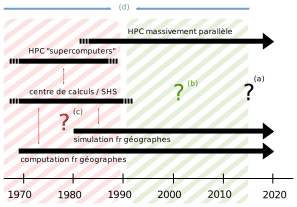
\includegraphics[width=.9\linewidth]{plan_HPC.pdf}
  \end{sidecaption}
\end{figure}

\begin{enumerate}[label=(\alph*),labelindent=\parindent,leftmargin=*]
\item En quoi est-ce un problème de ne pas s'intéresser au HPC depuis sa transformation entamée au milieu des années 1980 ?
\item Quelles pistes peut-on évoquer pour éclairer ce désintérêt d'une partie des géographes à l'encontre du HPC ?
\item En a-t-il toujours été ainsi ? Et, si ce n'est pas le cas, quelles traces trouve-t-on de ces pratiques et des challenges associés pour la simulation ?
\end{enumerate}

Une synthèse sera proposée en fin de section pour faire le lien entre ces différentes sous-sections.

\hl{ne pas tenir compte du point d) sur le schéma}
\hl{ne pas tenir compte du point d) sur le schéma}

%\item Pourquoi cette activité a disparu ? Est ce l'absence de  challenges à la hauteur en géographie ?

%En faisant le point de façon plus détaillé sur les pratiques informatiques de certaines équipes de géographes dans les centres de calculs, nous verrons d'une part que les challenges au delà de la micro-informatique continue d'exister bien après sa démocratisation, et que des tentatives d'explorations des modèles par l'usage d'algorithmes piochés dans les outils interdisciplinaire  comme l'exploration de modèle intervient immédiatement ou presque après  des retour vers le HPC entamé depuis 2010 au laboratoire Géographie-Cités des pratiques des modélisateurs de Géographie-Cités une pratique resté latente jusqu'à la redécouverte  on mettra en valeur les pratiques certains des usages ayant émerger dans les années 1980 au laboratoire géographie-cités, en explicitant
% Le point de vue d'Openshaw

\subsubsection{GéoComputation et HPC, quels enjeux pour la modélisation ? }
\label{sssec:enjeuxHPC}

Le mieux pour tenter de répondre, au moins partiellement, à cette première question, est de repartir des réflexions menées sur le HPC ces 25 dernières années par Stan Openshaw, Ian Turton et leurs collègues de l'école de Leeds. Ce qui n'était au départ qu'une intuition en 1983 \Anote{openshaw_intuition} devient très vite une réalité applicative en 1986 \autocite{Openshaw1988}. Basé sur l'usage du HPC et des techniques issues de l'IA (\textit{simulated annealing},\textit{genetic algorithm}, \textit{genetic programming}), Openshaw introduit dans son système AMS \textit{Building an Automated Modelling System to explore a universe of spatial interaction models} une rupture dans la façon de construire, évaluer et de façon plus générale penser l'exploration de modèles de simulation en géographie; rupture qui fait d'ailleurs à cette période parfaitement écho aux nouveautés technologiques annoncées par les différents articles de Couclelis : Automates Cellulaires \autocite{Couclelis1985}, Intelligence Artificielle, etc. \autocite{Couclelis1986}

Le saut technologique et méthodologique permis par ce projet, ainsi que les autres projets développés en parallèle, finit probablement de persuader Openshaw et son équipe de l'étendue des possibilités bientôt offertes par l'accélération et la transformation que subit le HPC entre 1980 et 2000 (voir section \ref{sssec:Tournant1980}).

Cette réflexion, l'école de Leeds finit en 1996 par l'intégrer dans un nouveau paradigme pour la géographie, la GeoComputation \autocite[4]{Openshaw2000b}

\foreignquote{english}{GeoComputation is not just the application of computers in geography. Nor is it just about computation for its own sake. It is meant to imply the adoption of a large-scale computationally intensive scientific paradigm as a tool for doing all manner of geographical research. Some will now claim they have been doing GC for 10 or 30 years or more. This is certainly possible, but if they were then, until 1996, it was certainly called something else; terms such as mathematical modelling, simulation, statistical modelling all spring to mind. There are three aspects which makes GC special. Firstly, there is an emphasis on the ‘geo’ subject [...] Secondly, the computation subphrase in GC is also special. It is the intensity of the computation that is especially distinctive [...] Thirdly, just as important and maybe even more significant is the underlying mindset. Computation implies a very particular paradigm based on numerical approximation rather than analytical precision. It can be based on data-driven high-performance computer-powered inductive tools rather than data free, analytically based, deductive methods. It involves trying to compute solutions to problems that could not previously be solved at all. It is based on substituting vast amounts of  computation as a substitute for missing knowledge or theory and even to augment intelligence. It could be data driven in a data mining sense, or it could be entirely data free with large-scale computer experimentation being used as a purely theoretical tool for understanding how complex systems work via modelling and simulation of their dynamics and behaviours. }

Toute une partie de la mise en oeuvre de ce paradigme est supportée par l'usage démocratisé du HPC \autocite[17]{Openshaw2000}. \hl{verifier ref}

\foreignquote{english}{GeoComputation is a relatively new term invented(or first used in its current form) in 1996. It is defined as the adoption of a large-scale computationally intensive approach to the problems of doing research in all areas of geography, including many GIS applications, although the principles are more generally applicable to other social and physical sciences; [...] It involves porting current computationally intensive activities on to HPC platforms as well as the development of new computational techniques, algorithms and paradigms that can take particular advantages of HPC hardware and the increasing availability of spatial information.}

Déjà critiqué pour ses positions techniques un peu trop \enquote{innovantes}, Openshaw (p11) prend les devants en explicitant point par point dans son manifeste \textbf{ce que n'est pas} la GéoComputation.

\foreignquote{english}{To summarize, GeoComputation is :
\begin{itemize}
\item Not another name for GIS
\item Not quantitative geography
\item Not extreme inductivism
\item Not devoid of theory
\item Not lacking of philosophy
\item Not a grab-bag set of tools
\end{itemize}}

De par son aspect paradigmatique, et l'ouverture disciplinaire qu'elle défend, cette réflexion n'est pas limitée à une application en particulier, comme en témoigne cette liste d'opportunités très génériques supportées par le HPC :

\begin{enumerate}[label=(\alph*),labelindent=\parindent,leftmargin=*]
\item \textit{To speed up existing computer-bound activities so that more extensive theory-related experimentation can be performed or to enable real-time analysis of geoinformation;}
\item \textit{To improve the quality of the results by using computing-intensive methods to reduce the number fo assumptions and remove shortcuts and simplifications forced by computational constraints that are no longer relevant;}
\item \textit{To permit larger databases to be analysed and/or to obtain better results by being able to proces finer-resolution data and make good use of very large computer memory sizes, and finally;
\item To develop new approaches and new methods based on computational technologies to provide new analytical tools and models, both of which are going to be highly important in the geoinformation-rich world of the future.}
\end{enumerate}

Comme il le précise déjà lui-même, les gains supposés ne sont pas forcément immédiats, et certains nécessitent le développement, ou le redéveloppement de modèles ou d'algorithmes pour exploiter différents niveaux de parallélisme \Anote{dependent_application}. Dans le cadre plus restreint des modèles de simulations, nous nous intéressons principalement aux gains immédiats permis par \begin{enumerate*}[label=(\alph*)]  \item la réutilisation des modèles ou algorithmes originaux libérés des contraintes techniques d'autrefois (mémoire, processeur)  \item l'utilisation d'algorithmes récents pour résoudre des problématiques autrefois insolubles \item la désimplification des modèles ou protocoles d'explorations \end{enumerate*}

D'une certaine façon, la communauté des modélisateurs agents emprunte déjà dans certaines de ces pratiques des améliorations telles qu'elles sont décrites par Openshaw (a). C'est le cas par exemple lorsque \autocite{Brearcliffe2014} tente de reproduire (\textit{reproductibility} et non \textit{replicability} \Anote{reproduire_repliquer}) un des premiers modèles individu-centré développé en 1983 par Hogeweg et Hesper \autocite{Hogeweg1983}. Il est évident qu'une toute nouvelle exploration réalisée avec un micro-ordinateur d'un modèle autrefois développé sur un \textit{mainframe} doté d'un processeur à 25Mhz et 4 Mb de mémoire ne peut qu'apporter de nouveaux éclairages sur le fonctionnement du modèle. Il est en effet aisé de faire beaucoup plus d'exécution du modèle sur la même durée, et cela sans compter tous les bénéfices apportés par un tel changement de plateforme \autocite{Wilensky2007a}.

Faire le pari de la GeoComputation, c'est être plus audacieux, et ne pas seulement se contenter du HPC pour gagner du temps ou des exécutions, mais d'intégrer dans nos pratiques un style de pensée qui valide l'utilisation sur nos modèles de calcul difficile ou impossible autrement qu'en utilisant du HPC (b)(Openshaw parle de \textit{HPC-dependence} ). C'est encore dans ce cadre de liberté, en théorie illimité (il y aura toujours plus de processeurs, toujours plus puissants), que peut s'exprimer au mieux une certaine forme de créativité et d'innovation algorithmique, différente de celle plus contrainte de la micro-informatique \autocite[26-28]{Openshaw2000}. C'est le cas par exemple de la méthode \textit{Pattern Search Exploration} (PSE) développé par \textcite{Cherel2015}, qui peut nous donner une bien meilleure compréhension de la palette des dynamiques exprimables par ce modèle de simulation, et cela sans avoir à le re-développer, ou à lui ajouter des objectifs à atteindre susceptibles de contraindre trop fortement cette exploration. Qu'attend-t-on alors pour retester d'anciens modèles (Wilson ? Allen ?), car Openshaw nous indique que de nombreuses connaissances sont déjà là, et n'attendent qu'à être saisies avec de nouvelles explorations.

Concernant le dernier point (c), la simplification intervient déjà dans l'activité de modélisation KIDS/KISS, via le retrait de mécanismes inutiles, ou dans le choix du niveau d'abstraction considéré comme judicieux/suffisant vis-à-vis de la problématique donnée. En dehors du fait que la simplification soit déjà au coeur du processus général de modélisation, celle-ci est également bénéfique lorsqu'elle est motivée par une substitution, par exemple lorsqu'il s'agit de remplacer l'expression complexe d'une dynamique micro par une dynamique agrégée macro quasi-équivalente (on parle de \textit{surrogate model} lorsque la substitution est par exemple motivée par un gain en performance lors de l'exécution du modèle). Appliquée par contre à l'exploration des modèles, cette simplification est une contrainte dont on se passerait volontiers, car elle met en tension l'interprétation des résultats vis-à-vis d'une dynamique d'expression incomplète, ou incertaine.

Un exemple récent est donné dans l'exploration du modèle de simulation Luti MobiSim, développé depuis plusieurs années maintenant par l'équipe Théma. Déjà familière du mésocentre de calcul de Franche-Comté \autocite{Asch2012}, il est pourtant indiqué dans la thèse de \textcite{Hirtzel2015} soutenue en février 2015 une limite dans l'utilisation possible des infrastructures disponibles, les simulations s'exécutant seulement sur des machines de 12 coeurs (5h30 par simulation) ou 16 coeurs (6h30 par simulation). 8 machines ($ x 12$ ou $ x 16$ donc) permettaient de faire des simulations en parallèle pour un total de 25 jours de calcul, 790 simulations exécutées équivalent à 60000 heures de calculs cumulés pour l'analyse de sensibilité présentée. Hirtzel évoque dans sa thèse l'impact important qu'une telle contrainte a eu dans la préparation, la planification, et la simplification de cette analyse de sensibilité assez complexe devant évaluer l'interaction entre 79 paramètres. \Anote{hirtzel}

L'effort est certes déjà impressionnant, et il ne s'agit pas ici de critiquer une expérience aussi importante techniquement et méthodologiquement pour notre discipline; toutefois, au vu de la contrainte technique régulièrement citée comme un goulot d'étranglement important pour l'exécution de ce modèle, il me semble que cela soulève une question d'accès aux ressources informatiques de ce type en SHS en général. En effet, pourquoi se contenter de cette infrastructure limitée et ne pas directement \enquote{taper à la porte} des physiciens ou des biologistes disposant d'équipements nationalisés coûtant plusieurs dizaines de millions d'euros à l'achat (20 millions d'euros pour le lot de calculateurs Ada et Turing), qui seront très probablement remplacés dans un futur proche, et cela hors coût de fonctionnement ? \Anote{naive_eject_shs}

Une autre façon de prendre conscience de l'impact possible de cette ressource dans notre quotidien de modélisateur est de prendre le problème à l'envers, comme le propose \textcite{Openshaw2000}  \foreignquote{english}{ [...] how would do you research if that PC on your desk was suddenly 10000 times faster and more powerful. It is likely that some researchers would not know what to do with it, some would not want it, but some would spot major new possibilities for using the computer power to do geography (and geo-related science) differently.}

Avec l'effacement brutal d'un grand nombre de contraintes techniques s'ouvre la possibilité d'un tout nouvel horizon de pratiques. Cette idée d'une exploration des modèles de simulation plus systématique, intervenant quasiment sans délai entre chaque remaniement conceptuel ou technique du modèle, et cela durant toute la construction, devient possible. \hl{Amblard ?}

La possibilité d'une parallélisation à moindre coût rend également possible l'exécution et donc la confrontation de modèle de simulation en parallèle. Ce n'est plus un modèle consacrant une seule série d'hypothèses que l'on évalue, mais un ensemble d'hypothèses regroupées dans une famille de modèles dont on explore les combinaisons de façon concurrente et simultanée, fonction de la question et des données présentées. Une idée qu'avait déjà explorée Openshaw dans son générateur de modèles AMS en 1988 \autocite{Openshaw1988}, et que nous avons reprise sans le savoir à notre compte dans la progression opérée par notre équipe de modélisateur dans Geodivercity \autocite{Cottineau2014b}

Même sans avoir à réécrire nos modèles pour tirer meilleur parti d'un parallélisme potentiel et plus implicite (1 ville = 1 processeur par exemple), les gains sont déjà évidents si on se contente du niveau de parallélisme le plus courant en géographie aujourd'hui (une simulation = 1 processeur). Un modèle de simulation qui s’exécute en $5$ min sur $100$ villes pourra une fois ces mécanismes validés à cette échelle, être appliqué à une toute autre échelle géographique, en $5$ heures par exemple sur les milliers de villes françaises. Sur un micro-ordinateur disposant de seulement quelques processeurs opérant en parallèle, cette \textit{scaling capacity} du modèle est inenvisageable. Par contre, sur un environnement HPC composé de milliers de processeurs, cette durée de simulation est largement compensée par le nombre de simulations réalisables en parallèle, avec cet avantage qu'une application écrite pour tirer parti de ce parallélisme d'assez haut niveau reste valide quelque soit le matériel qui l'exécute. L'achat régulier de machines supplémentaires ou le remplacement du matériel existant par du matériel plus rapide provoque immédiatement un bond dans la durée d'exécution et le nombre de simulations qu'il est possible d'exécuter simultanément.

Avec la démultiplication des capacités de stockage mémoire des machines, et l'avènement de collections de données à des échelles toujours plus fines, d'autres opportunités s'offrent au modélisateur à la fois d'un point de vue de la modélisation (la portée des axes KIDS/KISS, Stylisé/Particulier \autocite{Banos2013a} est étendue par les capacités techniques ainsi augmentées), mais aussi de la méthodologie. Il est en effet possible d'inclure dans la démarche explicative habituelle des modèles de simulation intégrant des données empiriques de résolution spatiale beaucoup plus fines qu'actuellement. La possibilité de faire des aller-retour d'un niveau de résolution spatiale à un autre est un moyen de ré-évaluer et de confronter la pertinence des mécanismes implémentés et des valeurs de paramètres choisies pour questionner nos connaissances théoriques supposées de la réalité, à différentes échelles d'observations.

On voit également très vite l'intérêt que peuvent avoir ces deux arguments ( \textit{scaling capacity}, résolution des données toujours plus fine) dans le cadre de la micro-simulation qui s'attache à reproduire des phénomènes observés dans des sociétés reproduites grandeur nature \autocite{Sanders2006}, souvent très difficiles à explorer du fait de temps d'exécution important.

Des scénarii exposés ci-dessus, il faut encore ajouter cette possibilité, déjà exposée, d'utiliser d'anciens (plus rapide) ou de tout nouveaux (impossible avant) algorithmes tirant parti eux aussi de cette parallélisation des simulations pour les explorations. On pense par exemple aux analyses de sensibilités, aux algorithmes évolutionnaires, etc.

En plus d'offrir une solution relativement pérenne, cet état d'esprit n'impose pas forcément le remplacement de pratiques de modélisation déjà existantes sur micro-ordinateur, nous verrons comment plus tard. En résumé, pour Openshaw \foreignquote{english}{You start by tackling small and simple versions of a more complex problem and then scaling up the science as and when either the HPC systems catch-up or knowledge of algorithms, models, and theory start to show signs of being able to cope [...] \textbf{The message is smart small but think big}}

Cette façon de penser, il me semble que les géographes modélisateurs en ont saisi depuis quelques temps déjà certains points, avec le développement d'une réflexion géographique appuyée par la computation, et l'adhésion à cette plus grande famille des sciences dites de la complexité. Pour ne citer que l'évolution la plus récente, le passage au paradigme informatique Agent dans les années 1990 est clairement un apport technologique externe à la géographie quantitative, appelant un renouvellement des réflexions méthodologiques et théoriques \autocite{Sanders2006} qui va bien au-delà du simple constat technique. Un apport technologique qui a redonné corps à des voies déjà explorées, tout en offrant la possibilité de résoudre des problèmes techniques ou conceptuels autrefois insolubles en les abordant sous un nouveau jour (le paradigme objet/agent est - entre autre - bien plus flexible pour la représentation des interactions entre entités). Certes la révolution HPC d'après 1990 n'entre pas (encore) en ligne de compte, mais l'idée d'un dépassement par l'apport technologique est déjà là.

L'accession successive à de nouvelles technologies a toujours servi à développer un projet scientifique qui se nourrit de cette multiplicité d'approches. Il faut y voir un processus d'accumulation, et non pas une succession poussée par une mode ou une autre.

Si l'on prend l'exemple de la théorie évolutive des villes de Denise Pumain, force est de constater que pratiquement toutes les nouveautés, technologiques et/ou paradigmatiques susceptibles d'un apport théorique ou méthodologique servant cette théorie (et par extension les objets géographiques concernés), ont été mises en perspective de façon critique dans chaque publication : les outils statistiques unis et multi-variés, les analyses factorielles, les systèmes dynamiques non linéaires, les réseaux de neurones, les automates cellulaires, la modélisation agent, tout a été testé avant d'être intégré dans la boîte des outils potentiellement re-mobilisables. Car il n'y a pas une technique meilleure qu'une autre, mais bien une combinatoire de techniques uniques, constitutives d'un raisonnement scientifique, dans laquelle chacune peut exposer tour à tour de multiples facettes  + ref communauté jass.

Il n'est pas interdit donc de penser que les progrès de la computation, si l'on cherche bien, apportent toujours au modélisateur de son époque les moyens de devenir un meilleur aventurier, pour reprendre l'image de l'explorateur donné par \textcite[22]{Banos2013} ou encore en citant la vision Openshaw \foreignquote{english}{Computation permits the investigator to test theory by simulation, to create new theory by experimentation, to obtain a view of the previously invisible, to explore the previously unexplorable, and to model the previously unmodellable.}

En un sens, cette seule phrase me semble suffisante pour imager tous les espoirs que nous avons placés dans ces usages renouvelés du HPC pour l'exploration des modèles de simulations en géographie.

Pour \textcite{Openshaw2000}, tous ces nouveaux usages ont acquis une forme de matérialité dès que la démocratisation du HPC s'est enclenchée. Il suffisait déjà dans les années 2000 de quelques efforts pour saisir cette chance. C'est d'ailleurs tout l'enjeu de son livre co-publié avec Turton à cette période, lorsqu'ils proposent, forts d'une expérience enracinée dans les années 1980 et de multiples prototypes fonctionnels innovants, de former les géographes aux usages simplifiés du HPC en moins de 200 pages. Presque 15 ans plus tard,  pourquoi cet argumentaire, pourtant brillant, développé par les supporters de la GéoComputation, n'a pas été entendu et mis en pratique outre-Atlantique ?

%Pour de multiples raisons, dont certaines déjà évoqués par Openshaw en 2000 - et sur lesquels nous reviendrons indirectement en étudiant le cas francais - il semble malheureusement que ces appels soient restés vains en dehors du cercle des géographes de Leeds, et des participants majoritairement anglo-saxon (plus géomaticiens ? plus géographes ?) régulièrement présent à la conférence \enquote{GeoComputation}.


\subsubsection{Quelles explications possibles pour ce désintérêt envers le HPC après 1990 ? }
\label{sssec:desertionHPC}

Openshaw cite en 2000 un certain nombre de critères qui peuvent selon lui expliquer ce retard chez les Anglo-saxons.

\begin{enumerate}[label=(\alph*),labelindent=\parindent,leftmargin=*]
\item Jusqu’à récemment (1998 du point de vue de l’auteur), cette ressource n’était pas satisfaisante pour envisager une utilisation plus généralisée en géographie. Il est à noter selon lui que la plupart des usages du HPC en géographie ne permet pas un usage incrémental, et il existe un véritable seuil à partir duquel les ressources à disposition deviennent intéressantes. Il est vrai que la mémoire mise à disposition des géographes dans ce type de machine est par exemple un facteur important d’utilisabilité, car que cela soit pour l’analyse spatiale, la simulation, il est important de pouvoir utiliser et stocker un maillage spatial suffisamment représentatif de la situation étudiée.
\item  La critique de fond adressée aux quantitativistes en géographie depuis les désillusions des années 1970, et la montée en puissance de géographie(s) plus qualitatives.
\item L’absence de tradition dans l’utilisation de ressources de calculs importantes, et le peu d’applications sont en partie la conséquence des deux points suivants.
\item  Les objections philosophiques héritées des critiques du néo-positivisme ou positivisme logique, et la peur de ne pas arriver à concevoir l’outil technologique comme un support neutre : \foreignquote{english}{Computation is just a tool, and how the tool is used and what it is used for and the context in which it is used depend on the interests, skills, and value systems of the user, which are themselves grounded in contemporary society.}
\item La complexité \enquote{apparente} de la programmation et la nécessité d’obtention de nouvelles capacités qualifiées de difficiles par beaucoup de géographes ne programmant plus depuis longtemps.
\item Le fait qu’on puisse imaginer cette activité computationnelle comme un renoncement automatique à toutes pensées critiques.
\item Il n’y a aucun agenda de recherche et aucune ressource informatique mise à disposition des géographes pour s’initier ou encourager l’usage des HPC.
\end{enumerate}

L'histoire et le contexte anglo-saxon sont évidemment très différents du contexte français, mais les points évoqués ici par Openshaw forment toutefois une première liste à minima de pistes à explorer depuis notre position actuelle. Les limitations techniques (a), et le peu de projets (c) ont pu être un facteur limitatif évident jusqu'à la fin des années 1990, mais aujourd'hui ces arguments sont plus difficiles à mobiliser. C'est également le cas du dernier point (g), des appels à projets et des infrastructures sans précédent sont en train d'émerger ces dernières années à un niveau européen, la motivation des géographes pour intégrer ce type de projet devrait logiquement être beaucoup plus audible. Restent donc les critiques classiques (b)(d)(f), dont on s'apercevra par la suite qu'elles continuent d'être mobilisées pour freiner le retour pourtant nécessaire d'un débat sur les rapports de la géographie à l'informatique, un frein visible aussi dans les enseignements de cette discipline (e).

Pour comprendre de quelles limitations techniques il s'agit, il faut faire le point sur ce qui implique cette transformation touchant le HPC dans les années 1990. Une fois mise en perspective toute la difficulté pour un géographe d'accéder seul à ce type de ressources, il faudra bien se poser la question plus générale de l'autonomie que l'on veut donner aux géographes sur le plan des enseignements informatiques, avant d'imaginer dans la continuité de nos pratiques, une solution plus concrète.

\paragraph{Tournant des années 1990 dans le HPC}
\label{p:Tournant1980}

La plupart des informations historiques et techniques proposées ici sont tirées des ouvrages suivants \autocites{Fox1994, Fox1988, Seitz1985, CM2-1990, Lerman1993, Padua2011, Dietrich1984}[81-84]{Culler1998, Steele2011} ainsi que des \textit{Working Report} suivant \autocites{Athas1987, Su1987, Seitz1983, Seitz1984a, Seitz1984b} dont la liste plus complète est disponible sur le \href{http://authors.library.caltech.edu/view/person-az/Seitz-C-L.html}{@site} des archives de Caltech.

Entre les années 1960-1980 on peut encore parler d'une phase de recherches et d'expérimentations, avec la création et l'amélioration des premiers \textit{supercomputers} à processeurs vectoriels, particulièrement adaptés au calcul scientifique rattaché généralement à cette époque à l'architecture SIMD \Anote{simd_def} qui va ensuite dominer le marché du HPC jusqu'en 1990. C'est le cas plus particulièrement de ceux qui vont germer dans l'esprit de Seymour Cray : Le CDC 6600 premier processeur multi-coeur scalaire, le CDC Star-100 premier processeur vectoriel (1974), l'Illiac III puis IV (1965, abandonné en 1975) considéré comme le premier d'architecture SIMD \autocite{Muraoka2011}, et enfin le mythique Cray-1 de 1976 à  80 MHz. Mais il y a eu bien d'autres projets similaires durant ces années d'expérimentations comme cite \textcite[387-388]{Steele2011} : Solomon computer (1960's), Texas ASC (1966), Goodyear Staran ( SIMD array processor, 1972) , ICL Dap (SIMD array processor, 1972 papier, 1974 prototype, 1979 commercialisation) , % Goodyear MPP plus tard, basé sur staran.

%Sur une autre branche, les MIMD, de nombreuses expérimentations concernant les architectures multi-processeurs, et la gestion du parallélisme ont également lieu : D825 (1962), CDC 6500 (1966), Multics system (1969)

Sur la base de ces premiers super ordinateurs, très coûteux, des années pré-1980, le domaine naissant du HPC va connaître un certain nombre de révolutions entre 1980 et 1990.

Entre autres innovations technologiques, l'introduction progressive des microprocesseurs depuis les années 1970 va permettre d'aller beaucoup plus loin dans l'invention fin 1970, début des années 1980 de nouveaux paradigmes de construction pour les ordinateurs. %Le parallèlisme peut être pensé autrement, et s'appuyé sur la baisse des couts qui frappe l'industrie informatique dans les années 1980.

Danny Hillis publie dès 1981 un mémo au MIT donnant les concepts \autocite{Hillis1981} d'une nouvelle machine massivement parallèle nommée \textit{Connection Machine} (CM), qui va amener un certain renouveau dans la façon de penser ce type d'architecture SIMD.

Ce dernier travaille d'abord avec Minsky et Papert au laboratoire MIT sur le langage LOGO, avant de créer une société en 1983 \textit{Thinking Machine} commercialisant une série de CM (Connection Machine) d’architecture SIMD (puis MIMD \Anote{mimd_def}), dont le premier prototype est présenté à la DARPA en 1985, et la première livraison commerciale en 1986. Ces machines constituent une référence historique initiale importante dans la construction de machines composées de plusieurs milliers de processeurs. En misant sur des processeurs plus simples, mais plus nombreux, répartis en noeuds (4096 noeuds chacun comportant 16 processeurs, ce qui fait au total jusqu'à 65536 processeurs, non vectoriels, très simples de 1 bit / 4kbit mémoire pour la CM-1, une architecture SIMD à mémoire distribuée). Pour cela; il repense la façon dont les processeurs sont amenés à communiquer entre eux via des routeurs distribuant les messages de façon très efficiente sur un réseau spécialisé. Appuyé sur une topologie de connexion en forme hypercube (12-dimensions, $2^{12} = 4096$ noeud) intégrant naturellement une représentation sous forme de grille de n-dimensions (pratique pour la simulation 2D et 3D), alors classique de cette époque, de multiples moyens de communication entre processeurs sont mis à disposition des utilisateurs. Le premier donne accès à une communication aux processeurs voisins (16 sur chaque noeud) de façon directe sans passer par le système de routing (système North/East/West/South NEWS), et le deuxième permet d'accéder à tous les autres processeurs via les routeurs implémentés sur chaque noeud (un pour 16 processeurs). Un système de processeurs virtuel permet de s'abstraire du nombre de processeurs physiques, ce qui rend les programmes opérant sur cette machine fonctionnelle, quelque soit la configuration existante (en plus de temps si le nombre de processeurs est moindre que le nombre virtuel choisi par l'utilisateur). Ces techniques permettent de se focaliser non plus sur la puissance des processeurs (cf l'unique processeur vectoriel du Cray-1 par exemple) mais sur la flexibilité et l'efficience des communications entre ceux-ci.

Sachant que David Hillis s'est largement inspiré des travaux de Minsky et de son livre \textit{Society of Mind}, cette architecture n'est pas sans évoquer l'image idéalisée du fonctionnement d'un cerveau tel qu'on se la représente à l'époque en IA symbolique, les CM's ciblant d'ailleurs résolument ce type d'application avec l'implémentation machine d'une version spécialisée de lisp, le *lisp (star lisp). Ainsi même si ce type d’architecture SIMD (dominante sur le marché des HPC jusqu’aux années 1990) est généralement plus complexe à appréhender, la CM a par exemple été utilisée très tôt pour développer des applications rattachées aux systèmes complexes dans le cadre de l’\textit{Artificial Life} et des \textit{Complex Adaptative System} (CAS), car elle s’appuie dans sa construction (voir la participation de Feynamn, et de Wolfram sur l'architecture de la CM) sur la propriété de parallélismes propres aux automates cellulaires (1 processeur = 1 cellule/patch !) \Anote{CA_physical}. Les CM proposent certes une alternative intéressante par cette possibilité augmentée de parallélismes, mais elles brillent aussi par leurs performances, la CM-1 (prototype) de 1985-1986 , la CM-2 (commercialisation) de 1986-1987 (2.5 à 6 GFlops), la CM-5 (qui passe d'une architecture SIMD à MIMD, avec 1024 processeurs) est numéro 1 du premier \href{http://www.top500.org/featured/systems/cm-5-los-alamos-national-lab/}{@Top500} de 1993 avec 59,7 GFlops sur le Linpack test. En comparaison, à l'IDRIS en 93, le Cray C98 Axis avec 8 processeurs dépasse à peine les 7 GFlops.

Des travaux similaires ont également lieu depuis les années 1970 dans l’équipe de physiciens de Toffoli (en contact aussi avec les travaux du francais Yves Pommeau) au MIT, qui finissent par concevoir courant des années 1980 un hardware spécifique (CAM-6, CAM-8) pour paralléliser les CA en s’appuyant sur leurs propriétés fondamentales \Anote{ca_simd_avantage}.

En France, il existe également des développements similaires en physique, avec la famille de machines R.A.P (Réseau d’Automates Cellulaires) démarrée en 1986 à Paris, OUPPY à Marseille\Anote{ouppy_marseille}. Ces deux architectures différentes (voir \autocite{Hillis1981}) inspirées par les CA \autocites{Hillis1984, Hillis1989, Toffoli1987} et  issues de travaux démarrés au MIT, sont également utilisés pour des applications scientifiques similaires \autocites{Epez1993, Toffoli2005}. L’équipe de l’UCLA de David Jefferson et ses modélisations de fourmilières (Tracker, Genesys, AntFarm) utilisent une CM contenant pour la première fois plusieurs milliers de fourmis, un préalable pour observer des comportements auto-organisationnels. Ou encore la première version parallélisée du langage LOGO qui sera développé sur ce type de machine CM avant de passer plus tard sur Macintosh (Starlogo 1991). Au Los Alamos National Lab (LANL) Langton recrute Hiebeler\Anote{hiebeler_parcours} en 1989 pour travailler sur le logiciel \textit{CellSim} initié en 1988 et mis à jour jusqu’en 1990; Hiebeler possède une expertise sur les CAM-6, mais également sur les CM car il a travaillé à Thinking Machine entre 1991 et 1992, ce qui lui permet de développer une interface sur ce logiciel vers des machines de type CM. Ces deux types de hardwares seront voués à un échec commercial, pour des raisons diverses qui ne touchent pas forcément au seul aspect scientifique, car ces outils ont constitué de réelles avancées d’un point de vue de la computation scientifique aux moments où elles étaient disponibles.

Dans l'avalanche d'innovations ayant lieu dans le courant des années 1970-80 au niveau du software et du hardware (topologie hypercube, vlsi et microprocesseur, baisse des coûts de production, langage acteur \autocite{Hewitt1973}, Unix, etc. ), le paradigme de construction basé sur l'architecture MIMD \Anote{exemple_simd_mimd} connaît lui aussi un certain rafraîchissement au tout début des années 1980, bien avant la livraison de la première Connection Machine CM-1.

C'est le cas par exemple du prototype \textit{Caltech Cosmic Cube} dont la première version fonctionnelle est finalisée en 1983. Ce dernier est une architecture MIMD à mémoire distribuée, répartissant sur 64 noeuds un système contenant : un micro-processeur intel 8086, un coprocesseur 8087 pour les flottants, une mémoire propre de 128K, et 6 canaux 2Mbits/s pour l'envoi de messages selon une pile FIFO (\textit{First In First Out} ) aux autres noeuds dans une topologie hypercube. Chaque noeud ne possède pas encore de véritable système d'exploitation propre (128k étant trop limite pour envisager la charge d'un OS complet de type Unix), mais un ou plusieurs logiciels de routages qui prennent en charge la gestion des messages entre les noeuds, regroupés sous le nom de \textit{CrOS}. L'avantage d'une telle architecture est évident, car elle pousse le constructeur à s'abstraire toujours un peu plus de la partie matérielle; en effet en passant d'une gestion de messages entre processeurs purement électronique à une gestion purement logicielle, on peut envisager de changer plus facilement certains composants du système tout en conservant un logiciel d'échange de messages \enquote{assez} similaire. Ainsi cachée derrière cet acronyme \textit{CrOS}, la librairie de fonctions de transfert de messages va très vite s'étoffer et s'améliorer pour se diriger vers un système \textit{loosely synchronous} \Anote{loosely_sync} de plus en plus indépendant de la machine.  %La programmation de ce type de parallélisme reste toutefois beaucoup plus difficile à gérer que les systèmes SIMD des années 1980 disposant à leur sortie de langages aux primitives adaptés pour l'application aisé de ce type de parallélisme.

En un sens ce choix d'une gestion logicielle donne lieu à plusieurs logiciels, soit repris et améliorés à partir du premier CrOS du Cosmic Cube ( NX-$n$ de Intel , PSE de NCube , CrOS-$n$ de Caltech) ou de conception propre à d'autres formes spécifiques d'architecture MIMD à mémoire distribuée (Ibm EUI, Meiko CS, TMC CMMD, etc.). Évidemment incompatibles entre eux, cette variété de matériels et de logiciels préfigure l'expression chez les utilisateurs d'un besoin rapide pour la constitution d'un standard/norme d'échange de messages implantés de façon transparente sur chaque machine : la norme MPI, dont on ne parle plus ensuite. Cette machine universitaire plusieurs fois améliorée de façon interne au laboratoire de recherche (Mark II (1984)/ Mark III (1986)) agrège autour d'elle plusieurs dizaines de programmes de recherches en tout genre, pour son utilisation ou son amélioration. Cette machine va également être déclinée dans des versions commerciales plus ou moins différentes (meilleurs processeurs, mémoire augmentée, ajout de composants pour réaliser des traitements spécifiques, utilisation d'Ethernet pour les échanges de messages, nombre de noeuds constitutifs, logiciels pour la gestion des messages différents, etc.) : nCUBE, Ametek, Intel iPSC, FPS T-Series, Paralex Gemini.

Autre avantage de cette machine, pour 1\% prix du Cray-1, elle produit 10\% de performance, ce qui prouve pour la première fois la faisabilité et les bons résultats d'une architecture parallèle utilisant des composants standards à moindre coûts. L'intel 8086 étant le premier micro-processeur de la famille x86 que l'on va retrouver dans une variante sur les IBM PC vendus dès 1981 à plusieurs millions d'exemplaires. %Sur la base d'une architecture MIMD à mémoire distribué la communication entre processeurs se fait sur la base d'une topologie en hypercube, avec un protocole d'échange de messages entre processeurs qui n'est plus piloté de façon physique par des routeurs, largement inspiré par la logique acteur de Hewitt.

On pourrait également citer par exemple les travaux sur le NYU Ultracomputer, de David E. Shaw sur la machine “Non-Von” (pour “Non Von Neumann”) de la Colombia University, le Goodyear Massively Parallel Processor (MPP), et probablement d'autres, moins connus. Toujours est-il que ces différentes initiatives sont toutes reconnues au début des années 1980 comme étant des pionnières dans la construction d’architectures \textbf{massivement parallèles}, c'est-à-dire mettant en oeuvre au moins plusieurs centaines de processeurs.

Touché avec l'apparition ou la maturation d'une véritable grappe de technologies durant les années 1980-1992 qu'émerge la notion moderne de cluster : les protocoles d'échanges de messages PVM puis MPI décrits ci-dessous, mais également Ethernet, le développement d'Internet, la miniaturisation constante et l'augmentation des fréquences d'horloges des processeurs, l'apparition de logiciels et de matériels libres, etc. que des projets émergent pour définir la notion moderne de \textit{cluster}. Ainsi cet esprit de réutilisation de \enquote{matériel standard} déjà expérimenté par l'équipe de Berkeley sur le \textit{Cosmic Cube} trouve son apogée dans l'invention plus ou moins simultanée de projets de mise en grappe de micro-ordinateurs dans les années 1990, en s'appuyant non plus cette fois-ci sur une architecture (\textit{hardware}) spécialisée reliant les différents composants (processeurs), mais sur leur simple mise en réseau appuyée par des applications (\textit{software}) de partage et d'échange de données efficient entre les machines.

%Cluster p292 / le projet NOW de Berkeley (NOW emphasized high-end workstations, high performance networks, and proprietary software) / et le projet Beowulf de la Nasa (Beowulf emphasized low cost personal computers, mass market networks (Ethernet), and the new trend in open source software including the Gnu editors and compilers and the Linux operating system)

Mais en dehors de ces applications et de ces architectures pionnières, d’un point de vue utilisateur la révolution opérée tient surtout de l’émergence et de la mise à disposition d’un plus large public de protocole de communication permettant de s’abstraire complètement de l’infrastructure qui supporte physiquement le parallélisme, que celui-ci opère sur un \textit{cluster}, ou sur des ordinateurs distants reliés par Internet, ou un mélange des deux. Ce type de norme a ainsi permis le développement plus aisé de programmes distribués de façon massivement parallèle, sans avoir à se soucier du langage à adopter, et de l’ensemble des contraintes techniques propres à chacune des technologies supportant ce parallélisme. Par exemple, la norme MPI (\textit{Message Passing Interface}) est devenue depuis sa création en 1992-1994 le modèle quasi-dominant implémenté (encore aujourd’hui) sur l’ensemble du matériel dédié à une utilisation partagée.

Ainsi, ces différentes visions d'une infrastructure support du parallélisme peuvent cohabiter et soulager l'utilisateur de la contrainte liée au hardware. Il est possible aujourd'hui de programmer un logiciel qui marche tout à la fois sur son propre \textit{cluster} personnel construit à base d'Arduino/Raspberry/Edison, que sur des architectures techniques plus complexes mélangeant différentes technologies ou paradigmes choisis pour une utilisation adéquate. Ainsi, les supercalculateurs d'aujourd'hui sont souvent eux-mêmes des formes de clusters, à la fois héritiers des premiers prototypes expérimentant des combinaisons de \textit{hardwares} et \textit{softwares} innovants, mais également héritiers de toutes les avancées liées à la démocratisation qui touchent l'ensemble des aspects matériels et logiciels dans l'informatique.

Le calculateur Turing de l'IDRIS \Anote{idris} est une architecture massivement parallèle (MPP de type \textit{MIMD distributed memory} \autocite{Snir2011}) cumulant de très nombreux noeuds de calcul (6.144 noeuds de 16 coeurs à 1 Go de mémoire par coeur) pouvant être connectés selon de multiples topologies. Celui-ci peut être accédé comme une seule et même machine (jusqu'à 65.536 coeurs simultanés autorisés en exécution). En comparaison, le \textit{cluster} ADA dispose d'une mise en réseau locale très rapide de plusieurs centaines de noeuds de calculs séparés : 332 noeuds d'architecture type \textit{Symmetric MultiProcessor} SMP) qui mélange deux types d'architectures : \textit{MIMD shared memory} sur le SMP et \textit{MIMD distributed memory} pour assurer la communication entre les SMP. Chaque noeud dispose d'un ensemble de processeurs multi-coeurs (32 coeurs) avec une mémoire partagée plus importante (4 à 8 Go par coeur), ce qui fait de ce calculateur ADA une architecture multi-processeurs destinée à des calculs plus communs (jusqu'à 2048 coeurs autorisés en exploitation), tout en restant très facilement extensible via l'ajout de nouveaux noeuds.

Comme on peut le voir dans les quelques paragraphes ci-dessus, le jargon technique (SIMD, MIMD-SH, MIMD-DM, DMM, SMP, etc.) qui accompagne l'environnement du HPC est un préalable à l'utilisation probablement rédhibitoire pour qui s'intéresse au HPC sans être du domaine.

\textbf{Mais, a-t-on besoin de tous ces détails techniques et de ce jargon ?}

Comme le dit si bien Openshaw (p6-7) \foreignquote{english}{We really do not need a whole lot of unnecessary details from computer science and computer engineering. Why not simply take it for granted and concentrate on using the technology? [...] Geographers should be viewing parallel computing as a tool that can be used on their problems; there is absolutely no need to know more than about 0.01 percent of the technical details of how the hardware actually works}

Ce qui nous amène à l'utilisation de ces différents types de ressources groupées sous le terme très générique d'HPC. Pour ce qui est des ressources pilotées par GENCI, toutes les demandes passent par un dossier administratif indiquant la nature du projet scientifique et la demande d'attribution d'heures correspondantes. Les projets doivent être déposés plusieurs mois à l'avance, avant d'être approuvés par un conseil scientifique réuni une à deux fois par an \autocite{GENCI2015}. Sur le \href{https://www.edari.fr/}{@site} de Demande d'Attribution de Ressources Informatiques (DARI) qui accueille les dépôts de dossier GENCI, on trouve la liste des 11 comités d'évaluation existant en 2015, et comme on peut le constater, il n'y a tout simplement pas de comité réservé pour les sciences humaines et sociales : Environnement, Ecoulements non réactifs, Ecoulement réactifs ou/et multiphasiques, biologie et santé, astronomie et géophysique, physique théorique et physique des plasmas, informatique algorithmique et mathématique, dynamique moléculaire appliquée à la biologie, chimie quantique et modélisation moléculaire, physique chimie et propriétés des matériaux, nouvelles applications et applications transversales du calcul.

Là encore, nous sommes très éloignés des pratiques, mais également des besoins pour la modélisation en SHS. Si on regarde à l'inverse du côté des sciences physiques, ce type d'accès est tout à fait normalisé, l'attribution du temps de calcul faisant souvent partie intégrante du projet de recherche déposé par les étudiants. Il existe aussi des encadrements dédiés pour les scientifiques ou les étudiants voulant apprendre à manipuler ces ressources. La \enquote{Maison de la Simulation} dispose par exemple pour les travaux pratiques de ces formations d'un accès dédié aux ressources HPC disponibles sur le campus du plateau de Saclay. C'est le cas aussi de l'IDRIS qui met à disposition des usagers du CNRS des formations dédiées. \Anote{formation_idris}

Si on regarde du côté des services offerts par un autre type de ressources HPC, les grilles de calculs (\textit{Grid Computing}) offrent une flexibilité d'emploi qui s'avère en revanche très intéressante, et cela malgré des limites évidentes pour certains usages.
% A reintegrer.
Elles offrent le plus haut niveau de parallélisme envisageable, et permettent de partager des exécutions de calculs sur des ressources complètement hétérogènes distribuées n'importe où sur la planète, en communiquant avec elles via Internet. Cette ressource ne fournit pas de mémoire partagée et/ou de mécanisme de partage de données entre les différents noeuds, considéré comme autonome, ce qui limite leurs utilisations dans le cadre de certaines applications nécessitant à la fois beaucoup de mémoire partagé, une communication forte entre les différents noeuds de calculs, ou et un niveau de parallélisme interne au programme : c'est le cas par exemple des astrophysiciens travaillant sur des modèles de simulation de l'univers composés de plusieurs milliards d'étoiles en interaction.

Il existe effectivement différents niveaux de granularité envisageable quand on parle de paralléliser des applications :
\begin{itemize}[label=\textbullet]
\item le parallélisme peut être envisagé de façon interne au niveau des primitives
\item le parallélisme peut être envisagé de façon interne au niveau des objets
\item le parallélisme peut être externe au programme
\end{itemize}

Les niveaux ne sont pas exclusifs, et une application peut très bien cumuler ces différents niveaux. Toutefois le parallélisme le plus simple et le plus immédiatement disponible consiste pour le modélisateur à attribuer un noeud de calcul par simulation, donc il s'agit d'un niveau de parallélisme externe au programme.

De multiples équipements informatiques implantés et accessibles à des mailles géographiques différentes, d'utilisation pour la production ou la recherche, sont réunis et accessibles aux chercheurs par le biais de divers portails administratifs. Appelées Organisation Virtuelle (\textit{Virtual Organization}), ces entités administratives virtuelles régissent l'attribution des ressources de la grille de calcul en fonction des différents accords passés entre les acteurs intervenant dans la constitution de la grille. Divers critères rentrent en jeu dans ce découpage, ceux-ci peuvent être de nature thématique, technique,selon des zones géographiques, politique, etc.

En France,depuis 2010 c'est le GIS France-Grilles (vo.france-grille.fr) qui mène cette mission de mutualisation entre les différents acteurs publics (Laboratoires, Méso-Centres, Centres nationaux) et privés au niveau national (Initiative Nationale de Grille ou NGI), mais aussi européens en étant le partenaire et représentant francais de l'EGI (European Grid Infrastructure). Piloté par des institutions scientifiques majeures (MESR, CNRS, CEA, INRA, INRIA, INSERM, CPU, RENATER), ce Groupe d'Intérêt Scientifique (GIS) coordonne la mise en place d'une grille de calcul nationale a priori accessible à toutes les disciplines scientifiques par le biais de différentes VO. D'après les statistiques 2012, sur 700 utilisateurs regroupés en 89 VO rattachées à la VO France-Grilles, seulement 12 utilisateurs sont enregistrés dans la catégorie systèmes complexes, et 0 pour les sciences sociales. Sur 1450 référencements entre 2010 et 2013, la collection HAL maintenue par France-Grilles pointant les publications utilisateurs de cette grille nationale, il y avait une seule publication référencée en sciences de l'homme et de la société. Aujourd'hui il y  a environ une dizaine de publications référencées, provenant en majorité de géographes.

Dans le cadre des SHS en France, il y a également la mise à disposition de ressources informatique de ce type, notamment par la collaboration au CNRS entre le \href{http://cc.in2p3.fr/}{@CC-IN2P3} et l'ancien TGE Adonis devenu TGIR \href{http://www.huma-num.fr/}{@Huma-Num}. Human-Num offre une liste de service à disposition des laboratoires, dans lequel figure un accès à des ressources informatiques de type grille de calcul, traitées par le biais de l'IN2P3, et accessibles via la technologie \textit{Grid-Engine}.

Pour utiliser tout ou partie de ce type de ressources HPC, il faut que le laboratoire d'accueil soit rattaché à une de ces entités administratives virtuelles, qui pourra ensuite délivrer un certificat d'accès unique au futur utilisateur (fichier crypté contenant une clef unique personnalisée reconnue par les machines de la grille), renouvelable tous les ans. GRID2-FR est l'autorité de certification du CNRS, le laboratoire doit être enregistré auprès de cet organisme pour pouvoir ensuite récupérer des certificats. La ressource est donc disponible de façon illimitée et relativement immédiate dès lors qu'on possède l'un de ces certificats. La ressource rattachée à chaque VO est généralement partagée avec l'ensemble des différents utilisateurs de celle-ci, même s'il peut exister dans certains cas des systèmes de quota. Une fois inscrit dans une VO, le laboratoire désigne une personne de confiance capable de signer et de délivrer des certificats de façon locale au laboratoire. Le processus pour délivrer les certificats est complexe, mais reste en définitive beaucoup simple qu'un dépôt de dossier administratif et scientifique ensuite jugé par un conseil scientifique thématique, comme c'est le cas via GENCI \autocites{GENCI2014,GENCI2015}. Intégrée par une seule personne, la procédure paraît d'un point de vue utilisateur moins coûteuse (pas de dépôt de dossier scientifique), et très simple (la demande d'attribution et la réception du certificat se font directement par Internet).

Ces modalités d'accès sont donc beaucoup plus intéressantes du point de vue d'un modélisateur dont l'activité de construction nécessite d'évaluer très régulièrement ses modèles de simulation par l'usage de techniques diverses, toutes relativement exigentes sur les aspects computationnels : analyse de sensibilité, plan d'expérience divers, usage d'algorithmes d'optimisation pour la calibration ou l'exploration des comportements du modèle, etc.

En résumé, nous nous intéresserons principalement par la suite aux \textbf{grilles de calculs}, car :

\begin{enumerate}[label=(\alph*),labelindent=\parindent,leftmargin=*]
\item La finesse de parallélisme engagée dans cette architecture est largement suffisante pour engager une première étape dans la voie du HPC immédiatement bénéfique pour la simulation en géographie,
\item On a accès à une ressource globale masquant l'hétérogénéité du parc de machines qu'elle représente, ce qui en fait potentiellement une ressource en constante évolution/amélioration
\item Les modalités d'accès à cette ressource sont plus compatibles avec les pratiques réelles des modélisateurs
\end{enumerate}

Mais il y a un hic dans tout cela. Si l'émergence, l'amélioration successive, et le maintien ces 20 dernières années de la norme MPI comme un standard indétrônable dans l'industrie du HPC a certes beaucoup simplifié les prérequis nécessaires pour user de ces ressources, le 0.01\% d'Openshaw inclut forcément des bases en informatique, ne serait-ce que pour comprendre et utiliser les fonctions MPI implémentées dans un langage de programmation, quelqu'il soit.

Des formations sont évidemment ouvertes dans ces différents instituts, mais non seulement ces organisations ne sont pas connues de la plupart des géographes, et de plus le niveau technique nécessaire à la compréhension de ces formations est trop complexe et trop éloigné du domaine de compétence des géographes pour que ceux-ci s'y présentent spontanément.

Autrement dit, et sans cette formation, une fois l'utilisateur connecté à une ressource HPC, quelle que soit sa forme, que se passe-t-il lorsque le curseur du terminal informatique clignote dans le vide? Quels sont ensuite les manipulations, les commandes, les fonctions à connaitre, à appeler, à intégrer dans nos programmes pour exécuter nos calculs, nos simulations en parallèle sur ces infrastructures ?

Même dans le cadre d'une mise à disposition pour les SHS, la ressource est fournie sous sa forme la plus brute \Anote{human_num_note}. On imagine qu'il y a peu de monde disposant, sans projet ou structure interdisciplinaire associée, du niveau suffisant pour mettre en oeuvre l'amorce technique nécessaire à la bonne utilisation de cette ressource informatique.

En définitive, et malgré des efforts conséquents des géographes de l'école de Leeds \autocite{Openshaw2000} pour introduire le HPC et la norme MPI aux géographes dans les années 1990-2000, on ne peut pas vraiment dire que cette pratique se soit diffusée outre-Manche ces 15 dernières années (et peut-être même en dehors d'un cercle très restreint des géographes informaticiens de Leeds).

Faut-il donc persévérer dans cette voie, ou existe-il aujourd'hui des solutions alternatives pour amener le HPC jusqu'au bout des doigts des géographes modélisateurs ?


%\item Des logiciels permettent de s'abstraire de la couche de programmation MPI normalement nécessaire pour accéder à ce type de ressources HPC,

%https://hal.archives-ouvertes.fr/FRANCE-GRILLES
%https://hal.archives-ouvertes.fr/FRANCE-GRILLES/search/index/q/%2A/domain_t/shs/
%GRID2-FR

%MPP p574

%Distributed Memory = Chaque processeur a sa mémoire propre, et peux accéder à la mémoire des autres via une forme de connection (réseau local, réseau spécialisé, bus spécifique, etc.)

%Blue Gene L = Distributed Memory MIMD computer

\paragraph{Quelle place pour les débats sur la place de la \enquote{pensée informatique} dans la géographie ?}
\label{p:Tournantenseignements}

Comme le disait déjà Michel Serres en 2011 dans sa séance d'introduction aux nouveaux défis de l'éducation \enquote{Avant d’enseigner quoi que ce soit à qui que ce soit, au moins faut-il le connaître. Qui se présente, aujourd’hui, à l’école, au collège, au lycée, à l’université ?} \autocite{Serres2011} A tous ceux qui pensent la programmation comme un apprentissage hors de portée de nos étudiants en licence, il faut leur ouvrir les yeux sur ce nouveau monde, celui bien réel décrit par Michel Serres dans \enquote{Petite Poucette} \autocite{Serres2012}, celui des étudiants qui se présentent aujourd'hui dans nos enseignements, et sur les initiatives de ceux qui ont déjà compris qu'apprendre à programmer était une activité aujourd'hui accessible dès le plus jeune âge.

Si l'on prend l'exemple d'autres pays, comme aux États-Unis en 2013, lorsque le président Obama prend la parole pour la \textit{Computer Science Education Week} organisée par la fondation \href{http://code.org}{@code.org} créee la même année : \foreignquote{english}{If we want America to stay on the cutting edge, we need young Americans to master the tools and technology that will change the way we do just about everything.} Si l'on peut regretter que cette initiative soit portée essentiellement par les fonds de grandes sociétés informatiques américaines, force est de reconnaître que l'intention politique est bel et bien là. D'autant plus que ce type d'initiative est loin d'être isolé, aux États-Unis, mais également sur la scène internationale. En France un réseau gagnant peu à peu le territoire est en train d'émerger, dans différents lieux d'accueil (bibliothèques, musées, FabLab, réseau des cantines numériques, écoles d'informatiques, clubs, etc.), des regroupements d'initiative locale, ou nationale.

Par exemple, l'initiative \href{http://Simplon.co}{@Simplon.co} \Anote{simplon} créée par \textcite{Bardeau2014} (le livre est conçu comme un manifeste pour \enquote{Lire, Ecrire, Compter, Coder}), est une entreprise au format juridique original (modèle ESS hybride : une entreprise solidaire d’utilité sociale agréée et une association d’intérêt général) qui propose des formations intensives de 6 mois pour les moins de 25 ans, sur dossier, quelque soit leur parcours scolaire. Récemment reconnue et soutenue par le gouvernement comme d'intérêt général, cette initiative en train d'essaimer un peu partout en France n'est qu'une parmi des centaines d'autres initiatives aux origines, aux formes différentes, mais aux objectifs communs : \enquote{La programmation pour tous}. Ce même groupe tient par exemple un annuaire \autocite{Simplon2015} qui compte aujourd'hui plus de 42 ressources différentes (club, réseau, écoles, sites, événements, etc.) à destination de l'apprentissage pour la programmation chez les plus jeunes, et ce n'est évidemment qu'un échantillon.

Autre exemple, l'initiative des enseignants néozélandais de \textit{Computational Science Unplugged}, qui donne corps au principe universel de \enquote{pensée informatique} (\textit{Computational Thinking}) au travers d'un livre d'activités illustré, pensé pour être utilisé par tout le monde, déjà traduit\Anote{traduction_unplugged} en plusieurs langues \Anote{texte_csunplugged}

En France, il aura fallu l'émergence spontanée et de plus en plus évidente d'un réseau fait d'initiatives citoyennes, la pression d'une communauté internationale bien plus au fait de ce mouvement, et l'échec répété de plusieurs projets nationaux, pour qu'en 2012-2013 soient \textbf{ enfin consolidés des instances (Conseil National Numérique) et une politique nationale à ce sujet}.

Les lignes énoncées par l'Académie des Sciences en 2013 (\enquote{L’enseignement de l’informatique en France. Il est urgent de ne plus attendre} \autocite{AScience2013}, ou encore les différents rapports du récent Conseil National du Numérique (dont le dernier Jule Ferry 3.0) \autocite{CNNum2014}, les soutiens solides entre ces acteurs \Anote{appui_academie_science}, les lettres ouvertes répétées des associations comme la Société Informatique de France \href{http://www.societe-informatique-de-france.fr/lettre-ouverte-a-monsieur-francois-hollande-president-de-la-republique-concernant-lenseignement-de-linformatique/lettre-ouverte-a-monsieur-francois-hollande-president-de-la-republique-concernant-lenseignement-de-linformatique-2/}{@SIF},soutenues et relayées par l'association quadragénaire spécialiste de ces questions \textcite{EPI2014}; \textbf{ces écrits sont unanimes, il faut agir au plus vite pour dispenser un véritable enseignement informatique, et former ainsi des citoyens qui seront acteurs du monde numérique}.

La réforme en cours pour le collège a annoncé très récemment (\autocite{SIF2015} 18 mai 2015) des pistes concrètes qui rejoignent les lignes énoncées \Anote{extrait_CNN} par le Conseil National du Numérique dans son dernier rapport \autocite{CNNum2014}. Reste à voir quels moyens effectifs seront annoncés pour mettre en place et pérenniser véritablement ces annonces :
\begin{itemize}[label=\textbullet]
\item Une initiative au codage dès le primaire
\item La programmation informatique au collège
\item une nouvelle option informatique en seconde et en première
\end{itemize}

Un projet dont il faut espérer qu'il ne sera pas abandonné au prochain mandat, car ce n'est pas la première fois que de telles annonces jalonnent l'histoire assez chaotique des relations entre l'éducation, l'informatique et les politiques \Anote{historique_EPI}.

\textbf{Quid de l'université et des sciences sociales dans ce mouvement ?}

Pour le moment, il est triste de voir que les initiatives prises dans l'enseignement supérieur de la recherche, comme celle de \enquote{France Université Numérique}, ne perçoivent cette révolution que sous l'angle unique du MOOC et d'un usage finalement très partiel et passif des technologies au service de l'éducation. L'avenir nous dira donc si cette prise de conscience finira par toucher un système universitaire, pour le moment absent dans ce débat.

Il existe déjà des filières spécialisées dans l'enseignement cumulé des mathématiques et de l'informatique pour les Sciences Humaines et Sociales (MIASHS), offrant des parcours interdisciplinaires intéressants. Mais ce que nous disent aujourd'hui ces différents rapports et cette multitude d'initiatives citoyennes, c'est qu'il est tout à fait possible d'enseigner l'informatique et sa logique sans faire appel à un support mathématique, ou même à un langage informatique en particulier (de simples blocs peuvent suffire, à l'image de Scratch \autocite{Resnick2009}), des outils qui peuvent intervenir bien plus tard dans la formation.

On observe également depuis quelques années déjà l'émergence de la thématique \textit{Digital Humanities} dans les débats sur l'informatique et les SHS. Ce mouvement \Anote{definition_complexe} qui se fait avant tout l'écho d'une relation renouvelée des SHS au regard des évolutions touchant l'informatique \Anote{humanite_digitale_histoire} se retrouve aussi dans des structures fédératives où sont plus ou moins mises en valeur certaines composantes de ce mouvement. Le TGIR Huma-Num par exemple fait avant tout ressortir un projet dont les termes \Anote{huma_num} paraissent assez éloignés des problématiques de programmation, de simulation, ou même tout simplement de calcul, alors même qu'il existe dans le giron de cette infrastructure des utilisateurs potentiels ou déjà actés de ce type de ressource : ALPAGE \autocite{Costa2012}, EQUIPEX MATRICE, GeoDiverCity, etc.

En effet même si cette dernière est bien retenue dans la grille de services proposés par le TGIR \Anote{human_num_note}, elle semble d'une part très peu valorisée dans les formations et les guides pratiques proposés par la structure, et d'autre part largement insuffisants pour des applications réelles, par exemple en simulation en géographie \Anote{human_num_notecout}.

Mais tout cela concerne la partie recherche d'un mouvement où l'heure en est encore au manifeste et à la réflexion, et dont on trouve extrait dans : Les discussions de la version française des \textit{Humanities and Technology Camp} \href{http://tcp.hypotheses.org/}{@ThatCAMP} et leur manifeste \autocite{THATCamp2010}, les livres comme celui de \textcite{Deuff2014} ou du collectif rassemblé autour de \textcite{Mounier2012}, le numéro 2 de la nouvelle revue électronique transdisciplinaire \href{http://rsl.revues.org/355}{@RSL}, le rapport commandé par l'Institut français \autocite{Dacos2015},  etc.

Il est donc encore assez difficile de voir quels impacts celui-ci a sur l'enseignement. On trouve toutefois une tentative pour le THATCamp2012 de \href{http://pireh.univ-paris1.fr/DHfrancophone/index.php?rem&val=g%C3%A9ographie}{@cartographie} des enseignements en humanité numérique sur la France \autocites{Berra2012b,Clavaud2012}, régulièrement mis à jour, et où semble-t-il aucune formation en géographie n'apparaisse. S'agit-il d'un retard de notre discipline dans l'intérêt qu'elle porte à ce type de mouvement, ou plutôt d'un effet de catégorisation lié au cloisonnement disciplinaire francais, la question amène probablement un débat qui dépasse de loin cette introduction. Parmi les rares acteurs de la géographie ayant pris conscience des enjeux scientifiques se cachant derrière cette première ouverture disciplinaire, on trouve une intervention de Thierry Joliveau à la conférence plennière du THATCamp de Lyon en 2014 \href{http://dhlyon.hypotheses.org/587}{@Video}).

Ces quelques pistes n'offrent qu'une entrée très limitée dans un débat méritant un travail de recherche plus conséquent, qui reste encore à faire. Il est difficile en effet de trouver une réflexion globale et actuelle interrogeant les rapports existants entre l'informatique et la géomatique, l'informatique et la géographie, la géomatique et la géographie, au niveau de la recherche et des enseignements, mais aussi dans la place que ces débats sont amenés à jouer dans celui plus large des humanités numériques.

%Quelle projection peut on faire au delà d'une utilisation passive du SIG, ou de la simple utilisation de logiciels de statistiques, une vision \enquote{utilitariste} de l'informatique dont on a vu qu'elle serait amené à changer.

Déjà cité comme étant un des rares géographes/géomaticiens étant intervenus dans les \textit{THATCamp}, Thierry Joliveau fait aussi partie de ces quelques scientifiques à même aujourd'hui de questionner l'actualité des relations entre géographie et géomatique. Dans le volume 5 de son HDR on trouve ainsi une section \enquote{Geomatique et géographie, débats et enjeux} qui ouvre une première réflexion sur ce sujet en 2004.

Dans son argumentaire, Joliveau n'hésite pas à s'appuyer sur le malaise et les querelles importantes soulevées par le SIG chez les Anglo-saxons dans les années 1990 \autocite[472-473]{Joliveau2004}. La lecture presque en parallèle des écrits d'Openshaw montre bien l'extension prise par ce débat entre informatique et géographie, loin d'être finie au tournant des années 2000. En effet, dans son manifeste pour le HPC \autocite[2]{Openshaw2000}, paru la même année que son ouvrage sur la GéoComputation \autocite{Openshaw2000b}, Openshaw et Turton n’hésitent pas à engager les géographes dans une métaphore qui les met en proie à une forme de maladie des plus virulentes. S'en prenant plus spécifiquement aux géographes \enquote{SIG-istes} (et accessoirement aux sciences sociales en général), c’est une forme particulièrement menaçante de \foreignquote{english}{let others do the programming for us} qui condamnerait peu à peu ces scientifiques à délaisser la programmation plutôt qu’à s’en emparer pour devenir acteurs de leurs propres outils \Anote{openshaw_virus}. Dans la continuité de sa guerre engagée contre les technophobes, Openshaw s'attaque  maintenant à une forme plus perverse de ce mouvement, celui-ci fustigeant l'immobilisme technologique et l'idée qu'on puisse penser l'outil et son utilisation comme une fin en soi. En se démocratisant, les outils deviennent d'une façon ou d'une autre bornés par les questions qu'ils permettent d'aborder. Il faut toutefois sortir de ce qui peut apparaître comme une fatalité pour l'étudiant, en lui donnant les moyens d'inventer seuls, ou avec de l'aide, ses propres solutions à ces nouvelles questions.

Bien que le contexte dans lequel le débat se pose initialement, et la forme prise en réponse aux critiques soit au final assez différente de l'autre côté de l'Atlantique, il semble bien qu'il y ait un socle commun à la base de cette prose critique questionnant les usages du SIG en géographie.

\enquote{Le débat dans la géographie anglo-saxonne traduit la réaction méfiante d'une partie de la communauté géographique par rapport à cette technoscience triomphante. C'est une réaction du même ordre qui a conduit les géomaticiens français issus de la géographie comme de l'informatique à veiller à se placer en dehors de cette vague de la géomatique \enquote{industrielle et commerciale} et à travailler en amont, sur des questions et des concepts, des méthodes ou des outils non pris en compte dans les produits logiciels du marché.}

Une méfiance, voire une prise de recul nécessaire, qui ne constitue pas en soi un problème, à condition toutefois de ne pas déroger à l'exercice nécessaire et légitime d'un questionnement scientifique sur le statut des connaissances ainsi produites par ce qui serait une nouvelle \enquote{ingénierie géographique}.

Sur ce point le débat reste ouvert, et Joliveau nous renvoie vers une lecture plus approfondie des positionnements épistémologiques empruntés par une GIScience anglo-saxonne, qui s'est depuis armée d'un discours en réponse à une \enquote{[...] tradition explicative de la géographie savante [...]} qui en général { [...] ne se satisfait pas d'un programme perçu comme essentiellement descriptif et principalement technique. La tradition critique de la géographie y voit même un projet dangereux} \autocite[474-477]{Joliveau2004}.

Concernant ce socle commun, Joliveau nous dit que \enquote{Les critiques des SIG du débat anglo-saxon auront sans doute rappelé d'autres débats plus anciens. P. George était parti en 1972 à l'assaut de \enquote{l'illusion quantitative en géographie} (George 1972). Il est frappant de constater que nombre de ses arguments correspondent point par point à ceux des critiques actuels des SIG. [...] 30 ans plus tard, certains continuent à s'inquiéter d'une dérive technique de la géographie à cause des SIG (voir plus loin).} \autocite[477]{Joliveau2004} L'auteur fait référence notamment aux velléités édulcorées (par rapport aux critiques anglo-saxonnes) et peu renseignées de \autocite{Staszak2001}. Mais pour Joliveau ce n'est pas tant le débat que l'absence de débat qui posent problème en France. La menace d'une dérive technologique sous-entendue par ces auteurs prend alors, au grand plaisir de ces derniers, des atours de prophétie auto réalisatrice \Anote{joliveau_texte}. Des auteurs dont Joliveau \Anote{joliveau_pgeorge} et Openshaw sont, il me semble, tous deux bien d'accord pour dire à propos de leurs discours que ceux qui s'y accrochent encore n'y connaissent en définitive absolument rien, et ne méritent donc aucun crédit.

%Alors même que la place du SIG fait parfois encore débats pour ce qui est de sa place dans l'enseignement - même si la situation s'est déjà grandement amélioré si on en croit Joliveau sur son blog en 2009 -, devrait on en plus se préparer à être totalement exclus de la majorité des futurs projets necessitant l’usage du HPC, c'est à dire de la programmation pour le HPC, en géographie ? Sans aucun doute, comme on l'a déjà remarqué au tout début de cette introduction.

Les enjeux semblent importants, et le débat passionnant. Presque 10 années plus tard, qu'en est-il de cet état de la question et de la place du SIG en géographie dans la recherche et l'enseignement ?

Au vu de la rapidité d'évolution des techniques, et de la démocratisation massive qu'a connue le SIG dans de multiples disciplines ces dernières années, il serait aventureux de se lancer dans une quelconque projection de cet état de fait datant de 2004, en 2015. On pourra par contre toujours se référer aux écrits pertinents de Joliveau et continuer ainsi à prendre le pouls d'un débat intervenant à la frontière du monde professionnel et universitaire, entre la géographie et géomatique, tel que développé sur son blog \href{https://mondegeonumerique.wordpress.com/}{@Monde-GeoNumérique}.

Il est intéressant par contre de prolonger les critiques énoncées en les transposant dans ce parti pris souhaité par Openshaw, celui d'un saut technologique supplémentaire, au-delà du SIG et même de la programmation, dans la maîtrise de la programmation spécifique au HPC. Car si ces critiques interviennent encore de façon dommageable dans l'intégration du SIG comme outil standard à disposition des géographes, alors il n'est pas difficile d'extrapoler, et de se dire qu'elles le sont probablement tout autant pour la programmation, et pour le HPC.

A ce stade, est-il possible d'envisager, comme Openshaw fait déjà état en 2000 pour les Anglo-saxons, un retard dans l'adoption du HPC en géographie en france ? Doit-on reprendre à notre compte ces craintes d'une géographie dépassée, en retard, oubliée, déjà avancées par plusieurs géographes dans le passé \Anote{joliveau_peur} ?

Ne prend-on pas le risque de passer à côté de thématiques comme le \textit{Big-Data}, les \textit{Smart-Cities}, qui engagent derrière cette couverture marketing des enveloppes d'argent importantes amenant la possibilité de traiter, et d’analyser des données géographiques récoltées à des échelles et avec des moyens inégalés jusque là ? Alors même que l’Europe est passée très près de débourser plus d'un milliard d’euros sur le projet FuturICT intégrant une très forte composante simulation, la programmation pour la modélisation est loin d’être couramment enseignée chez les géographes et les chercheurs géographes, quant à l'introduction aux moyens et aux techniques du HPC, celle-ci est quasi-inexistante, voire utopique. Doit-on s’attendre à voir ces précieuses données géographiques analysées comme de simples données \enquote{xy}, au détriment des géographes français et au profit de seules sociétés privées, surfant sur la vague des financements, et avec qui il faudra ensuite peut-être négocier pour accéder à ces données ?

%; c'est donc sans étonnement qu'on apprend les désagrement qu'a connu Openshaw avec les critiques dès la présentation de son prototype AMS.

En ce sens, l'urgence pointée par Joliveau de repenser le rapport de la géographie à l'informatique dans l'enseignement\Anote{formation_informatique} est essentielle pour le futur de la discipline, mais celle-ci dépasse de loin il me semble la seule question du SIG. Il ne s'agit pas simplement pour l'université de donner un débouché professionnel aux géographes en leur apprenant à programmer dans des master spécialisés - ce qui est un début, c'est vrai -, mais de leur donner de façon plus générale, comme on pu le faire pour les statistiques en leur temps, les bases suffisantes pour qu'ils puissent comprendre et améliorer les outils développés par les géographes dans le passé \Anote{aquoicelasert}, établir des collaborations actives et non plus passives avec les autres disciplines déjà rompues à l'informatique, mais aussi produire des outils de recherche en accord avec les développements de la société actuelle.

La plupart des auteurs abordant ce débat semblent d'accord, l'apprentissage de la programmation que cela soit pour la modélisation chez les géographes \autocite[64]{Banos2013}, dans les réflexions de géomaticiens \autocite{Joliveau2004}, dans les récits des géographes modélisateurs (Lena, Denise), en histoire dans l'enseignement \autocite{Genet1993}, ou encore dans le cadre plus large des humanités numériques \Anote{code_humanite}, dans le cadre des initiatives citoyennes, ou depuis peu dans les institutions, \textbf{l'apprentissage de la programmation n'est pas une fin en soi, elle est un moyen pour une fin} \textcite \autocite[67]{Plantin2014}. Elle est ce socle de connaissance initial, dont le contenu reste encore à définir, qui permet d'engager cette co-construction autour de l'informatique entre les disciplines.

L'accès à la programmation, ou du moins à la \enquote{pensée informatique} pour tous dans les filières universitaires, et plus spécifiquement en géographie (en dehors des seuls master spécialisés), est un projet qui est, semble-t-il, encore à construire.

%Tout comme Netlogo a su ces dernières années fédérer les modélisateurs, ce mouvement doit être de nouveau capturé dans la création d’un outil accueillant ces échanges pour ce qu’ils sont, c’est à dire bilatéraux (et non pas l’expression d’une commande), imparfait (car manipulant des concepts au sens différents, voire conflictuel), et imprégnés (il n’est pas facile d’adopter un nouvel angle d’analyse). L’objet de cette co-construction ne se concentre plus uniquement sur le modèle, mais sur l’exploration de celui-ci, et cela en utilisant tout la réunion des moyens humains et informatique faisant déjà usage du HPC.


%http://web.media.mit.edu/~mres/papers/designing-for-tinkerability.pdf

%Nous verrons par la suite que la solution proposé basé sur l'utilisation du logiciel OpenMOLE réduit encore un peu plus ces efforts, et vient s'accoler au plus pret des usages actuel chez les géographes modélisateurs.

% Seconde question

%\hl{transition transition transition}

Si le HPC est un acronyme à la définition relative, il doit être étudié \textit{in situ} pour mettre face à face challenges scientifiques et moyens computationnels  au moment où ils sont disponibles.

%On a bien vu dans le chapitre 1 que les géographes, et certains modélisateurs pionniers dans les sciences humaines, s'étaient déjà tournés vers ce qui était alors les rares et uniques ressources informatiques permettant d'être en adéquation avec les enjeux scientifiques en ces temps. Cette motivation, il me semble que les géographes l'ont trouvé déjà une première fois en françe dans les années 1970, dans l'application notamment de toute nouvelles techniques pour la statistiques ou la simulation, les deux marchant de paire avec la découverte de l'informatique.

%Nous verrons dans la section \ref{sssec:centre_habite} que ces traces existent, même si elles sont encore assez peu documentées.

Repris de façon hétérogène par les sciences humaines, l’usage de \textit{supercomputers} est resté pendant quelques décennies le premier contact \enquote{contraint et forcé} que ces pionniers ont eu avec l'informatique. A ce titre, le chapitre 1 a déjà donné un aperçu des nombreux travaux réalisés par ces chercheurs en sciences humaines, et il me semble important de re-souligner le courage qu'il a fallu pour braver à plusieurs, ou parfois seul, toutes les contraintes à la fois intellectuelles, financières et physiques permettant d'approcher de telles machines, avant tout construites pour les besoins des sciences physico-mathématiques.

En résumé, on pourrait donc arguer qu'il s'agissait \enquote{d'un autre temps}, et que le \textit{supercomputer} était alors le seul moyen de faire de l'informatique. Oui, c'est vrai, mais en partie seulement.

Pour mieux comprendre dans quel contexte nous nous situons, il faut tenter une immersion dans un monde quasi-dénué de toutes perspectives informatiques impliquant une utilisation autonome de l'ordinateur \Anote{gibson}. Difficile alors d'évoquer cette rupture conceptuelle et physique qu'a pu être l'arrivée de la micro-informatique dans certaines pratiques bien installées des sciences humaines. Tout d'un coup un objet un peu plus gros qu'une calculette apparait sur votre bureau, et permet de réaliser des calculs quasi-similaires à ce que vous faisiez en à peine quelques heures de plus sur des \textit{supercomputers}.

Considérée comme un événement bénéfique par quelques scientifiques déjà convertis à cette pratique de l'informatique depuis 10 ans, ou objet considéré comme inutile, décoratif, voire dangereux pour beaucoup; force est de constater que l'implantation progressive des \textit{micro-computer} dans les facultés au cours des années 1980 a quand même fini par rendre en partie obsolète une pratique de l’informatique jusqu'alors contrainte à l'utilisation des centres de calculs.

Toutefois, il ne faudrait pas se contenter ici de dérouler un argument trop commode, selon lequel dès lors que la micro-informatique apparaît, tous les géographes disparaissent des centres de calculs fréquentés auparavant.

Si la majorité des géographes vont effectivement se tourner vers la micro-informatique dès lors qu'elle se démocratise, on retrouve aussi dans plusieurs équipes des accointances plus ou moins durables avec certains centres de calculs, accointances dont on trouve encore trace physique aujourd'hui dans des politiques d'équipement, mais aussi dans la fréquentation ou la construction de structures d'accueil scientifique.

Pourtant, si l'on applique de façon rétroactive l'argument d'Openshaw faisant du challenge scientifique une nécessité motivant l'usage du HPC, alors il nous faut aller plus loin que ce simple constat et montrer en quoi l'apparition et la démocratisation des micro-ordinateurs n'a pas été un événement suffisamment convaincant pour que certaines équipes décident de continuer à pratiquer ces centres courant des années 1980-1990.

Une entrée même partielle dans cet historique des pratiques - tel qu'on s'y essaye par la suite dans la section \ref{ssec:hist_ccalcul} - permet à défaut de produire une étude exhaustive, d'apporter quelques éclairages sur cette question.

Devant les difficultés d'usages des moyens informatiques de l'époque, la mise en oeuvre apparaît en elle-même comme un challenge informatique nécessitant co-construction, au croisement des formations de certains universitaires à la programmation, et de la fréquentation de creusets interdisciplinaires dans, et/ou autour des centres de calculs, que cela soit en SHS, ou chez les géographes (Strasbourg, Besançon, Montpellier, Paris). Il faut rappeller qu'à cette époque, il est impossible d'utiliser un programme de statistiques, ou de cartographie sans avoir recours à des notions de FORTRAN.

Cette diversité des pratiques, des collaborations, est donc la preuve qu'il y avait dans la pratique de ces centres interdisciplinaires d'autres projets, d'autres challenges plus stimulants que celui du seul accès à une ressource informatique pour faire des statistiques. Car à y regarder de plus près, l'autonomie et l'indépendance permise par l'utilisation de cette nouvelle ressource micro, sont des qualités qui peuvent à l'inverse être aussi approchées comme une invitation au repli sur soi, à la dispersion des efforts impliquant l'apparition de \enquote{re-création informatique} stérile \Anote{remarque_informaticien_roue}, et l'effacement possible de ce riche horizon interdisciplinaire et de l'activité de co-construction qu'il supporte \autocite{Banos2013}.

En un sens il n'y a donc aucune raison pour que certaines de ces interactions interdisciplinaires, une fois nouées, ne disparaissent toutes subitement avec l'apparition de nouveaux logiciels ou de nouveaux équipements. Il est impossible de donner un point de vue global sur ce point, et nous verrons, comme l'a déjà noté \autocite[372]{Cuyala2014}, que les premiers géographes formés à la programmation informatique adoptent vis-à-vis de celle-ci, et par rapport à l'enseignement ou à leur recherche, des postures personnelles ou collectives tout à fait diverses. La seule chose que l'on peut avancer de façon plus certaine, c'est qu'il y a bien eu un jour la disparition des enseignements de programmation d'une partie des cursus de géographie quantitative, au profit de l'utilisation d'outils.

En résumé, le \textit{supercomputer} a continué à exister et à être accessible tant qu'il y a eu de la place pour les SHS dans les centres de calculs, certains géographes ont donc continué à l'utiliser, d'autres non, pour diverses raisons dont on donnera un aperçu dans la sous-section \ref{sssec:centre_habite}.

% Voir si le paragraphe ne meriterait pas d'etre plus haut

Concernant le cas plus spécifique de la simulation, nous pourrons d'ailleurs revenir plus précisément dans la section \ref{sssec:contexte_modelisateur} sur une série de collaborations entre géographes et physiciens/chimistes qui illustre ce que Denise Pumain décrit aussi comme l'assurance \enquote{de se donner des instruments à la hauteur des questions que l'on se pose}, preuve supplémentaire que les challenges scientifiques s'inventent aussi dans l'importation et l'adaptation de techniques et de méthodologies issues d'autres disciplines.

%Une matrice de 9 par 9 ou de 73 par 73, telle qu'elle est utilisée par exemple par Openshaw dans son générateur de modèle AMS \autocite[40]{Openshaw1988}, est intéressante d'un point de vue théorique, mais ne permet pas une montée en complexité suffisante permettant la comparaison avec l'empirie. Comme l'avait déjà souligné Openshaw, ce n'est qu'une fois enclenchée la transformation du HPC au milieu des années 1980 que certaines applications peuvent enfin dépasser le stade de prototype. On évoque dans la section \ref{sssec:Tournant1980} abordant plus en détail les changements opérant à cette période les difficultés d'usages par exemple des automates cellulaires sur de large grille.

%N'est on pas dans une situation similaire ou la construction et l'exploration de nos modèles de simulation est encore largement contrainte par les ordinateurs équipants nos postes de travails, et cela probablement pour encore quelques temps ?

% Rejoignant le constat du chapitre 1, cela prouve aussi que les sciences humaines et les géographes ont été capables d'apprendre l'informatique et de surmonter des obstacles bien plus importants que ceux pouvant se dresser devant nous aujourd'hui pour accéder au HPC (ce qui explique aussi le manuel d'Openshaw sur le HPC \autocite{Openshaw2000}, qui croyait vraiment à cette possibilité de dépassement dans la discipline), preuve que lorsque les enjeux scientifiques sont à la hauteur, rien n'est impossible.

\subsubsection{Un bref historique des usages du HPC en géographie et en Sciences Humaines et Sociales}
\label{sssec:histo_centrecalcul}

%Avant de revenir sur cette question, il est important de noter que ces centres de calculs, à la différence peut être de ce qu’ils sont devenus pour certains ces dernières années, sont avant tout des lieux propices à l’inter-disciplinarité dans les années 1970-1980.

% SMA encore existant ?
% PACTE : Sonia Chardonnel, Elise Beck

En 1984, à l'occasion du Congrès International de Géographie se tenant pour la première fois à Paris, \textcite{Faugieres1984} cite dans l'ouvrage de synthèse \textit{La recherche géographique Française} une enquête du CNRS daté de 1982 \Anote{bulettin_intergeo}. Il en tire les éléments suivants : sur 162 formations en géographie, ou dirigé par des géographes, 31 seulement ont pu founir des indications sur l'utilisation de moyens informatiques, 8 départements de géographie n'ayant aucune activité informatique. Sur ces 31, l'utilisation se répartit de la façon suivante, 9 utilisent des centres de calculs, 12 ont à leur disposition des terminaux, 2 ont accès à des \enquote{mini}, et 13 ont acquis un ou plusieurs micro-ordinateurs (23 au total).

En 1983, \textcite[367]{Lecarpentier1983} expose dans les \textit{Annales de Géographie} une première description technique du \textit{micro-ordinateur} et de ses avantages, en partie pour contrebalancer un usage de l'ordinateur en géographie qui selon-lui \enquote{ [...] reste donc marginale en regard des énormes possibilités offertes. En ignorant cet outil-là, après bien autres, la géographie laisse le champ libre autres disciplines plus réceptives à l'évolution des mentalités et des techniques. Souhaitons que ce numéro spécial des \textit{Annales de Géographie} soit l'occasion - et le signe - d'un renversement de tendance et passons en revue la tâche immense qui attend le géographe, s'il veut bien apprendre à utiliser l'ordinateur et notamment le micro-ordinateur autrement que de façon marginale et accessoire.}

Il commente également (p 348) les résultats d'une enquête auquelle il a eu accès pour fonder son analyse, sans donner les chiffres, mais qui tend à vérifier les conclusions donnés précédemment par Faugières (probablement la même ? \Anote{bulettin_intergeo_a} ) : \enquote{ Une enquête récente menée auprès de géographes universitaires français a montré que le recours au centre de calcul reste le moyen le plus répandu mais que utilisation du mini- ou du micro-ordinateur en est souvent complémentaire. Les grandes universités (Paris, Montpellier,  Grenoble, Strasbourg) utilisent surtout ou exclusivement leur centre de calcul et apparaissent sous-équipées en matériels spécifiques. Les micro-ordinateurs se diffusent rapidement un peu partout mais leur généralisation est gênée par l'absence de logiciels adaptés aux besoins des géographes Quelques équipes (Besançon, Lille, Rouen) ont entrepris la réalisation de logiciels de ce genre [...] Finalement, malgré sa diffusion rapide dans de nombreux secteurs d'activité, le micro-ordinateur reste un outil mystérieux et inconnu pour la plupart des géographes.}

Cette période des années 1980 reste d'approche assez délicate, car si les centres de calcul semble rester un pôle d'accroche important pour de nombreux géographes, elle est aussi marqué aussi par l’émergence à la fois externe de nombreux packages logiciels développés par une nouvelle industrie florissante du logiciel informatique, ou interne, par les développements de géographes devenu pour certain expert en programmation informatique. Pour \autocites[444]{Joliveau2004}{Waniez2010}, la diffusion de la micro-informatique et de logiciels plus évolués sur le plan graphique et de l’interaction homme-machine courant des années 1980 a ainsi rendu complétement obsolète l’usage des centres de calculs pour l’usage statistique et cartographique. Quid alors des autres usages ?

Pour appuyer les discussions sur cette époque, quelques témoignages ont pu être collectés durant le premier semestre 2015. Je remercie d'ailleurs par avance la géographe et professeur Colette Cauvin, le sociologue et professeur Philippe Cibois, l'historien et professeur Jean-Philippe Genet, l'ingenieur de recherche au CNRS Alexandre Kych, et la géographe et professeur Denise Pumain, et Lena Sanders pour les informations qu'ils ont bien voulu me transmettre sur ces pratiques pionnières de l'informatique dans les SHS, et plus spécifiquement sur les usages des centres de calculs alors à leur dispositions. Si l'apparition de non-géographes dans cette liste peut apparaitre comme étrange en premier abord, ces temoignages seront aussi l'ocasion de mettre en avant les autres \enquote{fonctions} supportés par ces lieux, qui reviennent souvent dans les témoignage comme les creusets d'une pratique solidaire et/ou interdisciplinaire de l'informatique. Les extraits qui viennent sont pour la plupart tirés de ces témoignages dont on trouve une reproduction intégrale en annexe de la thèse. \hl{ref annexe}

L'apprentissage de la programmation FORTRAN et la maitrise d'un contexte matériel complexe daté des années 1970 est un passage quasi-obligé pour la plupart des géographes francais voulant appliquer les techniques quantitatives. Cette aprentissage apparait nécessaire pour dérouler les programmes informatiques révolutionnaires venu des Etat-Unis \autocite[150,127]{Cuyala2014}, mais également pour exécuter les nouvelles statistiques uni et multivarié, quand ce n’est pas tout simplement pour maitriser à minima les entrées / sorties d’un superordinateur. Information difficile à trouver sans réaliser un travail historiographique important, la thèse de \textcite{Cuyala2014} nous donne quand même quelques informations sur le bagage techniques de certaines des premiers géographes quantitativistes francais : Sylvie Rimbert (formation au Fortran à Ottawa p 137) ;  Cosinschi, Racine, Lemay, Cavalier (formation Fortran à Ottawa p 150), Pumain ( Ottawa p 153), B.Marchand(p 154), Durand-Dastès (p 313) Dumolard (\hl{p?} ), et surement d’autres du fait de leur origine Quebecoise, de leur profils hybride, ou de leur attirances pour une certaine rigueur mathématique (p 157-158).

Pour introduire les usages de l'informatique et des centres de calculs chez les géographes dans les années 1970-1990, on fait appel à une typologie en trois classes introduite par \textcites{Wieber1980}[448]{Joliveau2004} : l’accès aux packages logiciels ou à la programmation directe en cartographie et en statistiques se fait soit en interne lorsque les équipes ou les universités possèdent du matériel, soit par un accès direct aux centres de calcul, soit par un accès indirect par des terminaux en contact avec ces mêmes centres. Si les la présence de centres à proximité des équipes coincident souvent, la qualité de l'activité ne saurait se rapporter à cette seule présence, ou à la taille d'une université.

L'innovation à Besançon tient par exemple de cette première catégorie. \textcite[131]{Cuyala2014} souligne l’importance des collaborations entre Jean-Claude Wieber, géographe alors issue de l’institut de géographie alpine sous le patronage éclairé de Paul Claval, avec le mathématicien Jean-Philippe Massonie.

%IBM 1630 ?
\textcite{Massonie1986} a créé le laboratoire Mathématique Informatique et Statistiques (MIS) en 1964. Implanté dans une UER de Lettres et Sciences Humaines à l’université de Franche-Comté de Besançon, ce laboratoire atypique accueille une inter-disciplinarité qui n'est pas seulement dirigée vers la géographie \Anote{massonie_texte}. Disposant d’un petit centre de calcul rattaché à l'UER, la présence initiale d'un matériel modeste (IBM 1130 jusqu'en 1975 \autocite[22]{Wieber1980}, puis IRIS 50, IRIS 80 plus puissant \autocite{Massonie1986}) n'empêche en rien l'innovation. Cette équipe fait tout à la fois partie des premières à user des toutes nouvelles méthodes statistiques \autocite{Massonie1971}, mais c'est également elle qui va impulser l'important colloque interdisciplinaire de Besançon à partir de 1972. Intitulé \enquote{L'application des méthodes mathématiques à la géographie}, ce lieu d'échange joue selon \autocite[331]{Cuyala2014} un poids indégnable dans l'histoire de la géographie quantitative française; on trouvera pour plus d'information un compte-rendu des dix ans d'activités dans les annales de géographie en 1983, deux ans avant sa disparition \autocite{Massonie1983}

Avant même le début des années 1980, ce groupe investira très vite dans du matériel micro-informatique, en partie du fait de nouvelles contraintes liées à l'utilisation du matériel, comme le laisse deviner le commentaire de Massonie sur sa page Internet personnelle à propos de l'IRIS \enquote{Cela devient un vrai ordinateur parce qu'on y a plus accès. La bête est enfermée dans une cage de verre, des techniciens le font marcher. Le matin on dépose ses cartes dans un bac, à midi on récupère les cartes et le listing des résultats. On a perdu le coté ludique. Les informaticiens ont pris le pouvoir. Certes il est plus rapide, mais que m'importe que mon calcul qui durait 1 heure, ne dure plus que 10 minutes, si je ne récupère les résultats que 3 heures après.} Un micro-ordinateur est acquis par Massonie dès 1978 pour développer \enquote{un logiciel d'analyse des données dont l'utilisation soit bon marché et accessible à des non-informaticiens.} Devant les performances satisfaisantes de ces micro-ordinateur, et l'autonomie qu'ils permettent, de nombreux logiciels micro sont adaptés ou créés à partir de là (ANACONDA, SADE, PATATE, etc.)\Anote{massonie_1978} \autocite{Massonie1986}. Cette volonté d'une \enquote{informatique conviviale} \autocite{TSH1984}, on la retrouve par la suite tout au long des transformation successives englobant ou accompagnant cette structure initiale originale.

Ce laboratoire a été le support dans la décennie 1980 d'un secteur de recherche (AMMSIOSHE) groupant plusieurs laboratoires (Géographie, Histoire, Littérature, Philosophie, etc.), mais également d'un GIS \enquote{Techniques nouvelles en sciences de l'homme} et d'un DEA pluridisciplinaire \enquote{Méthodes et Techniques nouvelles en sciences de l'Homme et de la Société} \autocite{TSH1984}. Le laboratoire MIS deviendra en 1997 le MTI SHS (Méthodologie et Technologies de l'Information appliquées aux Sciences de l'Homme et de la Société) \autocite{Girardot2004} et regroupera dans son projet l'ambition d'être à la fois une plateforme technologique, un lieu d'interdisciplinarité pour les sciences de l'homme et de la société, et un partenaire pilote dans la formation à l'innovation mêlant informatique et sciences humaines (ISTI). Après le départ à la retraite de Jean-Philippe Massonie, ce projet interdisciplinaire construit sur 30 ans se poursuit également avec l'émergence d'un nouveau projet scientifique autour de la MSHE C. N. Ledoux (2002), structure commune aux deux universités de la région \autocites{Favory2003, Favory2009}. Le MTI SHS est aujourd'hui intégré comme équipe de recherche technologique (ERT) pour l'intelligence territoriale au sein de l'UMR multi-site Théma créé en 1999, qui participe également dans certains pôles de la MSH de Dijon et de la MSHE Ledoux de Besançon. Cette MSHE sert une optique mutualiste, avec la mise à disposition des autres disciplines de services humains et matériels appartenant initialement à Théma. La structure de la MSHE Ledoux dispose en effet en 2015 de ses propres calculateurs de taille moyenne (PowerEdge R815, Dell Précision 7500) destinés aux traitements locaux de données lourdes, preuve aussi que cette \enquote{culture du centre de calcul} reste une condition importante dans la marche d'un environnement interdisciplinaire. Une remarque aussi à mettre en perspective du tout centralisé, et de l'absence d'équipements similaires dans d'autres MSH en sciences humaines. Il existe également un partenariat entre ce laboratoire et le mésocentre (centre de calcul régional) de Franche-Comté \autocite{Asch2012}, sur lequel par exemple tourne la plupart des simulations du modèle LUTI Mobisim.\autocites{Thema2010, Hirtzel2015}

Le pôle strasbourgeois impulsé par Sylvie Rimbert regroupe à partir de 1968-1969 Etienne Dalmasso, Monique Schaub, Colette Cauvin \Anote{informations_colette_cauvin}. En 1970, le statisticien et débutant en informatique Michel Pruvot intègre l'équipe à son retour du Canada, également complété en 1971-72 par Gérard Schaub, puis Henry Reymond en 1973 \autocite[135-153]{Cuyala2014}. De retour du canada, ce dernier remplace Etienne Dalmasso alors nommé à Paris. L'équipe active en statistique informatique est principalement composée de Michel Pruvot, Colette Cauvin, Sylvie Rimbert et Henri Reymond. %@bla

Fort d'une formation à l'étranger pour certains, apprentissage initié ou complété par les formations du CNRS (1971 à Strasbourg, 1972 à Paris) pour d'autres, ce petit groupe est en tout cas très rapidement opérationnel en informatique, en statistique et en cartographie, dès le début des années 1970. C'est cette triple compétence qui permet à l'équipe d'utiliser au mieux et très rapidement les ressources informatiques à leur disposition sur le campus universitaire de Strasbourg. En 1971, deux projets sont finalisés, une des toutes premières applications d’ACP sur un milieu géographique intitulé \textit{Essai d’application de quelques méthodes statistiques à la région milanaise} \autocite{Dalmasso1971}, mais également une commande d'atlas informatisé pour l'agence d'urbanisme de la ville de Strasbourg. Un véritable tour de force chez les géographes de cette époque, car ce travail s'appuie sur l'utilisation dès le dernier trimestre 1970, des ressources informatiques mis à disposition par le Centre de Calcul de Strasbourg-Cronenbourg (CCSC) créé sur le campus en 1968-69 pour les besoins de la physique.

C'est grâce aussi à la collaboration régulière avec Anne Engelmann, une physicienne et informaticienne du CEREG disposant d'un bureau au CCSC, que les géographes de cette équipe vont accéder à la fois à des facilités matérielles \Anote{collette_ccsc_centre} et logicielles; une collaboration qui s'inscrit physiquement dans un lieu où on ne s'attendait surement pas à voir y résider de façon durable des géographes. Ainsi outre les bibliothèques logicielles déjà accessibles aux utilisateurs du centre, comme BDMP par exemple \Anote{bdmp_package_strasbourg}, Anne Engelmann a assuré plusieurs installations de logiciels à destination des géographes : le logiciel SYMAP (1965) d'Harvard dont une version en Fortran a été apportée par des étudiants canadiens entre 1970 et 1971, divers logiciels de cartographies achetés ou récupérés par Sylvie Rimbert entre 1973 et 1979, etc.

Alors que l'arrivée de la micro-informatique dans le laboratoire se fait de façon progressive à partir de 1982-1983, les activités de programmation peuvent se diversifier, sans mettre en danger semble-t-il cette liaison avec le centre de calcul. Une fréquentation du centre qui restera continue jusqu'à la fermeture du centre en décembre 1993, avec l'organisation d'enseignements, et/ou la mise en oeuvre d'activité de recherche impliquant l'installation, l'utilisation ou le développement de logiciels. En 1985-90, l'activité des géographes de Strasbourg se développe même sur un double lien, avec la mise en oeuvre d'une liaison avec le CNUSC (Centre Universitaire de Calcul du Sud), essentiellement motivée par des collaborations du GIP RECLUS initiées par les géographes de Montpellier (on on parle un peu plus loin).

Michel Pruvot développera des logiciels sur les différents équipements micro successifs du laboratoire, alors que Colette Cauvin et Sylvie Rimbert, bien qu'écrivant également de petits programmes, préfère mettre l'accent sur le dialogue et la co-construction avec les développeurs spécialistes de l'équipe. C'est le cas avec Anne Engelmann, mais également avec deux scientifiques rodés à l'informatique ayant rejoint l'équipe dans les années 1970. Ingénieur d'étude puis de recherche, Jacky Hirsch intègre l'équipe dès 1977 (avec des contacts dès 1976), et dispose aussi comme Engelmann d'un bureau au CCSC. Autre ingénieur d'études devenu chercheur par la suite Charles Schneider travaille essentiellement dans le groupe de Sylvie Rimbert sur de la cartographie et de la télédétection.

Ces derniers ne se contentent pas de développer et fournissent également un support humain (enseignements, formations) et informatique important aux deux équipes du laboratoire, celle de Sylvie Rimbert mais également celle de géographie quantitative. Les deux ingénieurs écrivent également des logiciels ensemble, comme en 1983 le logiciel de télédetection Cartel sur l'Univac 1100 du centre.

C'est Colette Cauvin qui gère les relations et les finances du centre pour les étudiants jusqu'à sa fermeture et son remplacement en 1994 par le Centre Universitaire Régional de Ressources Informatiques (CURRI) dans le nouvel ensemble universitaire de l'ULP à Illkirch, un Centre de Ressources Informatiques (CRI) ou celle-ci occupe les mêmes fonctions\Anote{calcul_curri}.

Il faut en effet rappeler que l'institut n'a disposé de véritable salle pour la micro-informatique que vers les années 1987-88, des appareils utilisés en premier lieu pour les cours de statistiques.

Les autres cours, mais également une partie des logiciels de l'équipe implémentés initialement sur les \enquote{grosses machines} du centre de calcul, doivent donc s'adapter très régulièrement au changement de matériels informatiques qui touche le centre : en 1968-69 un IBM aurait apparemment existé, remplacé dès 1970-71 par un Univac 1108 \textcite{Dalmasso1971}, un Univac 1100 en 1983, puis au plus tard en 1985 un IBM3060/IBM3090. Ce dernier système marque la fin des perforatrices et l'arrivée de terminaux interactifs IBM 3179 \autocites{Rimbert1984,Cauvin1986}. Un peu plus tard encore, l'arrivée progressive de terminaux à l'université va permettre à l'équipe de se connecter au centre distant de quelques kilomètres. Une évolution qui rend enfin possible l'exécution d'un certain nombre d'opérations à distance, les listings résultants étant renvoyés par le centre deux à trois fois par jour.

Bruno Guérin développe également des logiciels servant pour l'enseignement de l'analyse spatiale sur un \enquote{Amstrad}. Colette Cauvin qui dispose d'un \enquote{Vic} personel, l'apporte en cours pour certains TP entre 1982 et 1985. Ainsi Michel Pruvot, initialement responsable des enseignements de statistiques au CCSC, se met rapidement au développement de logiciels de statistique sur micro-ordinateur et sur Macintosh dès qu'ils sont disponible. C'est lui également qui conçoit et gère la première salle d'informatique en libre d'accès pour les édutiants en 1987-88, il y donne les TD de statistiques sur des logiciels qu'il a pour la plupart lui même développés, et cela dans un but avant tout pédagogique. A coté de ça, les chercheur s'équipe peu à peu de logiciels achetés (Carto2D, MacGrizdo, etc.), ou développés par Michel Pruvot, avec l'arrivée de matériel Macintosh dans le laboratoire. Il y'aura également l'arrivée de un ou deux PC, cloturant ainsi l'équipement disponible jusqu'en 1993-94.

En dehors des formations en statistiques qui vont basculer sur les micro-ordinateurs lorsque ceux-ci seront disponible, la plupart des formations, comme les stages, puis les cours de cartographie démarrés au centre en 1973-1974, et ceux de télédétection démarrés en 1982-1983 se feront toujours au centre jusqu'à sa fermeture en 1993. Avec comme on a vu des adaptations majeures, les perforeuses ont été remplacées par des terminaux plus récents, les programmes ont souvent été réécrits plusieurs fois, avec comme on a commencé à le voir l'arrivée de développeurs ou l'amélioration des compétences de certains chercheurs en informatique ayant permis le développement de programmes propre aux besoins d'enseignements et de recherches. Ainsi, dès l'arrivée de Jacky Hirsch, celui-ci développe (parfois avec l'aide d'étudiants, comme Aziz Derradj, enseignant en cartographie aujourd'hui) des logiciels spécifiques à partir de librairie acquise par le CCSC (par exemple la librairie d'application graphique danoise Uniras acquise en 1979-80) ou de tout nouveaux logiciels comme Cartel, justement créé pour les stages de télédetection. Ces logiciels sont souvent également utilisés dans le cadre des recherches menées par les différentes équipes du laboratoire.

Avec la fermeture du CCSC et le passage au CURRI, la plupart des enseignements et des travaux de recherche ont pu continuer grâce à l'adaptation des logiciels faite par Jacky Hirsch. Ensuite le laboratoire s'est peu à peu équipé de logiciels PC (cartographie, statistique, SIG) de tout type, pour l'enseignement ou la recherche, par exemple en 1994 Arc/Info (enseignement et recherche) et Idrisi (surtout pour l'enseignement). Le centre de calcul CURRI est quant à lui resté nécessaire pour avoir accès à des logiciels comme SPAD, Hercule, ainsi que pour la télédetection jusqu'au début des années 2000, avant l'achat de logiciels spécialisés.

% le seul on imagine à disposer de l'équipement adéquat pour les sorties de logiciels de cartographie.

A Grenoble (H. Chamussy , P. Dumolard, M. Durand, Joël Charre part à Avignon par la suite, Maryvonne Le Berre part à Besançon par la suite) c’est l’Institut de Géographie Alpine (IGA) qui se coordonne avec le Centre Inter-universitaire de Calcul de Grenoble (CICG, formalisé en 1972). Le modèle AMORAL développé par une partie des membres de cette équipe a été écrit dans le langage DYNAMO, après l'impulsion donnée par François Rechenman de l'IRIA, et Patrice Uvietta du laboratoire Atelier de Recherches sur les Techniques Mathematiques et Informatiques de Systemes (ARTEMIS) de l’Institut d'Informatique et de Mathématiques Appliquées de Grenoble (IMAG). A la fin des années 1989, Joël Charre et Pierre Dumolard, qui bénéficie chacun d'un bagage informatique solide (Dumolard à fréquenté le CICG assidument peu après son ouverture \autocite[323]{Cuyala2014}) qui se chacun rapidement spécialisé dans la micro-informatique, mettent à disposition des géographes le logiciel INFOGEO en 1989 \autocites{Charre1989,Theriault1989,Ferrier1991}.  %Ce dernier intervenant également de façon plus générale chez les géographes par le biais de son inscription au groupe DUPONT, et dans la participation aux différentes formations associées à cette période à l'analyse de systèmes en géographie, comme celle par exemple organisée par Guermond en 1982 \autocite{Guermond1984}.

Le pôle d'informatique grenoblois, et notamment l'IMAG, est historiquement lié à l'émergence de la discipline informatique comme science du même nom en France. Une des impulsions importantes est donnée par l'universitaire Grenoblois Jean Kuntzmann dans les années 1950, ce mathématicien et supporteur précoce de l'analyse numérique va militer pour la création, la formation, et la diffusion de ce qui va devenir par la suite l'informatique. Celui-ci est le fondateur et dirigeant de l'IMAG jusqu'en 1977, un des premier laboratoire associé au CNRS, disposant d'un rayonnement international y compris sur le plan non-académique. Au milieu des années 1960, le laboratoire emploi 140 personnes, dont 60 doctorants. Si le Centre Inter-Universitaire de Calcul de Grenoble (1972) n'est vraiment officialisé qu'en 1972, de nombreux ordinateurs analogiques (1951), puis digitaux(Gamma ET, Marchant 10FA en 1957, IBM 7044 et 1401 en 1963, IBM 360-67 en 1968) seront amenés à passer bien avant dans ce premier Centre de Calcul. En 1977, cet effectif se porte à 300 personnes. Celui-ci est également le créateur de l'Association Française de Calcul (AFCAL) en 1957 qui deviendra par la suite AFCALTI, AFIRO, puis l'AFCET (Association Française pour la Cybernétique), dont les colloques et conférences ont constitué un des canaux importants de diffusion de la systémique dans le milieu scientifique et technique, y compris en géographie quantitative \autocite{Pumain2003}. Il n'est donc pas étonnant de voir l'utilisation appliquée de systèmes dynamiques émerger de ce centre en particulier, car Kuntzmann lorsqu'il créé l'Ecole Nationale Supérieure d'Informatique et de Mathématiques Appliquées de Grenoble (ENSIMAG) lui insuffle cette volonté d'une mathématique, et d'une informatique résolument tournée et enrichit en retour par des applications, car \enquote{Il ne faut pas séparer une science de ses applications; à longue échéance, les mathématiques coupées des applications deviendraient stériles.} \autocites[422]{Mounier2012}{Chiffres1977}

\begin{table}[!h]
	\centering
	\begin{sidecaption}[fortoc]{Une idée des ressources informatiques disponible au CNRS, de l'IBP à l'IDRIS. Les sources pour construire ces deux tableaux proviennent de \autocites{CNRS1972, Boucher2000, Mounier2010}}[tab:machines_circe]
		\begin{minipage}{1\textwidth}
			\centering
			\subbottom[]{
				\begin{tabular}{@{}cll@{}}
				\toprule
				\multicolumn{3}{l}{A l’Institut Blaise Pascal IBP ( 1946 - 1969)} \\ \midrule
				Entrée      & Identifiant machine      & Remplacement         \\ \midrule
				1955        & Elliot 402               & (1962)               \\
				1957        & Gamma 3, AET             & ( ? ,  ?)            \\
				1958        & IBM 650                  & 1966                 \\
				1961        & IBM 1401                 & ?                    \\
				1962        & Elliott 803, IBM 704     & ( ? , 1964/1966)     \\
				1963        & CAB 500, IBM 1401        & (? , ?)              \\
				1966        & CDC 3600                 & ( 1972 )             \\ \bottomrule
				\end{tabular}
		 	\label{machines_a}}
		 \end{minipage}\qquad
		 \begin{minipage}{1\textwidth}
		 	\centering
			\subbottom[]{
				\begin{tabular}{@{}cll@{}}
				\toprule
				\multicolumn{3}{c}{Au CIRCE ( 1969 - 1993 ) à Orsay} \\ \midrule
				Entrée   & Identifiant machine      & Remplacement   \\ \midrule
				1965     & Univac 1107 (Faculté)    & 1968           \\
				1966     & CDC 3600, IBM 360 / 40   & (1972, 1967)   \\
				1967     & IBM 360 / 50 et / 75     & (1972, 1972)   \\
				1968     & Univac 1108 (Faculté)    & 1970           \\
				1969     & IBM 360/75               & (1972, 1972)   \\
				1970     & Univac 1106 (Faculté)    & ?              \\
				1972     & IBM 360/20, 370/165      & ( ?, ?)        \\
				1985     & AMDAHL 470/V7, NAS9080   & (?, ?)         \\
				?        & IBM 3090/200             & ?              \\ \bottomrule
				\end{tabular}
			\label{machines_b}}
		\end{minipage}
  \end{sidecaption}
\end{table}

%IBM 704 : 20 KIPS/12 kFLOPS
%CDC 3600 : 1.3 MFLOPs
%CRAY1 : 160 MFLOPS

%http://www.tablesgenerator.com/latex_tables

% A l’institut blaise pascal ( 1946 - 1969) :
% 1957 :  un  Gamma  3  puis  un  AET.  De  Possel,  chef  du  labo  à  l' IHP,  passe  à  l' IBP.
%  1958 :  un  IBM  650 ;  de  Possel  devient  directeur  de  l' IBP.
% 1961 :  un  IBM  1401
%  1962 :  un  Elliott  803  (acheté  1  MF)  puis  une  IBM  704
%  1963 :  une  CAB  500  et  une  seconde  1401
%  1964 :  une  CDC  3600,  remplaçant  la  704
%  1966 :  une  IBM  360 / 40  à  disques  et  bandes,  dans  le  nouveau  local  du  CIRCE  à Orsay
%  1967 :  une  IBM  360 / 50  remplaçant  la  prècédente

% Au Circe (1969 - 1993) :
% Univac 1107 -> 1108 (1968)
% Univac 1106 (1970)
% CDC 3600 (1968-1972) et IBM 360/75 ( ?- 1972), IBM 360/20, 370/165 (1972 - ?)
% 1985 : AMDHALV7 et NAS9080
% IBM 3090/200

% A l’IDRIS (1993 - maintenant ):
% Vectoriel Cray C98 (en 1993) et Cray C94 (en 1994) jusqu’à 2000
% Cray T3D fut installé en 1995
% Cray T3E en 1996
% 2001 IBM Power4
% etc.

%http://pireh.univ-paris1.fr/mv/num9.html

Le Centre de Calcul de l'université Paris 1 dépend depuis sa création de l'UFR d'économie, sous la tutelle originale du professeur Claude Fourgeaud.

Ce centre était situé au sous-sol du Panthéon rue Cujas, à la fac de droit, au pied du grand escalier. Celui-ci était composé d'une salle avec l'ordinateur local, et d'une autre salle, plus petite, ou deux femmes étaient responsables de la perforation des cartes pour les utilisateurs et les chercheurs. Un bac était à disposition des envois de cartes perforés pour execution au Centre Inter-Régional de Calcul Electronique (CIRCE, voir tableau \ref{tab:machines_circe}) à Orsay  \Anote{remarque_denise_centrecalcul}. C'est ainsi que les premiers calculs statistiques sont réalisés par les géographes, par exemple lors des cours de 1969-1970 de Bernard Marchand ou les étudiants sont amenés à apprendre le FORTRAN avec l'aide d'informaticiens, les cartes perforées des étudiants finissant dans ce bac, avant d'être envoyé au CIRCE pour execution \autocite[127]{Cuyala2014}.

Parmi les utilisateurs les plus assidus du centre en SHS, alors en libre service pour les enseignants chercheurs, il y'avait semble-t-il l'historien Jean-Philippe Genet, les économistes Pierre-Yves Hénin et Michel Pouchain, et enfin les trois géographes Thérèse Saint Julien, Denise Pumain, et Yvan Chauviré.

A son arrivée à Paris 1 en 1969-70, l'historien médiéviste Jean-Philippe Genet précédemment formé à l'informatique par l'équipe de Marc Barbut à Paris 5, indique la présence au centre de calcul de Paris 1 d'un IBM 1130 assez poussif, assez vite remplacé par un Philips P880.

D'autres utilisateurs sont également amenés à travailler au centre, par exemple pour encadrer des développemements ou des utilisateurs, pour des logiciels génériques, ou pour des applications plus spécifiques.

Denise Pumain parle ainsi d'\enquote{un groupe d'informaticiens et de mathématiciens-statisticiens (dont Yvonne Girard) préposés à aider les usagers du centre de calcul situé au Panthéon.} Pour Genet, en dehors de cette tutelle des économistes, assez peu visible, le fonctionnement du centre au quotidien était principalement assuré par la mathématicienne Yvonne Girard, et ce groupe des plus assidus, toujours prêt à s'entre-aider.

Genet cite également dans le personnel actif, l'importance de Jean-Paul Trystram, un directeur de recherche à l'IRIA (ex-INRIA) ayant travaillé au centre avec Xavier Debanne, créateur par la suite du logiciel BDP (Banque de Données Paris 1), une forme de logiciel type SPSS qui sera longuement utilisé dans ses différentes versions sur le Philips P880.

Genet dont le niveau en informatique n'est pas forcément suffisant pour développer de nouveaux logiciels, fait appel au professeur de Paris 1 et militaire Édouard Valensy pour lui fournir des ingénieurs collaborateurs dotés d'un haut niveau informatique, comme Jacques Mondelli ou François Hucher. \Anote{pionnier_genet}

Ce dernier estime que le centre de calcul lui a été utile de son arrivée en 1970-1971 jusqu'aux années 1985-1990 environ, période à partir de laquelle il est devenu beaucoup moins intéressant d'utiliser cet équipement. Il aura fallu ce temps-là pour que les logiciels soient convertis ou achetés sur micro-ordinateur, et que les chercheurs s'équipent, souvent à leurs propres frais, entre autre du fait d'une absence (volontaire?) de politique générale du CNRS. A partir de 1987 certains départements d'histoires reçoivent une circulaire annonçant l'implantation de micro-ordinateur. Une décision qui s'est faite sous l'impulsion de Jean-Pierre Bardet, un historien démographe de Paris 4 ayant travaillé avec Genet. Une fois Bardet entré au Ministère de la Recherche comme chef de mission scientifique, celui-ci décide de changer les conditions de travail des historiens par cette expérience pilote. Une avancée qui ne prolongera pas, comme en témoigne cet appel d'urgence pointant l'insuffisance des équipements chez les historiens en 1993 \autocite{Genet1993}. % Ajout ref http://pireh.univ-paris1.fr/mv/num9.html

Dans le cas de l'UFR d'Histoire de Paris 1 c'est quand même douze Bull 45 (ou Bull 35, selon le témoignage) reçu en 1987 qui ont permis aux historiens de relâcher l'usage du centre de calcul, et de relancer en 1989, dès qu'une salle a été trouvée pour les installer, une UV d'histoire et d'informatique permettant une formation plus systématique des historiens à cette matière. En effet, le centre de calcul étant réservé avant tout au chercheur, la formation lancée par Genet en 1975-1976 (ou 1978-1979 selon le témoignage), utilisant le centre de calcul normalement limité aux chercheurs, est interrompu, et cela apparemment jusqu'en 1989. En juillet 1993, cette salle sera rééquipé avec dix PC 386 SX, un changement qui fait figure d'exception dans cette situation de crise, comme il a été pointé dans le paragraphe précédent \autocite{Genet1993}.

Parmi les autres utilisateurs du centre figurent les membres de la future équipe P.A.R.I.S (Denise Pumain, Thérèse Saint-Julien, et plus tard Léna Sanders) qui n'hésite pas à mobiliser les ressources offertes par le centre soit pour la réalisation d'analyses statistiques, soit un peu plus tard pour des modèles de simulations (cet usage sera détaillé en particulier dans une prochaine section)

A son retour du Canada en 1969-1970, Denise Pumain fait en effet partie du groupe de géographes autonomes capables de programmer en Fortran. Alors que Genet semble alterner pour ses recherches entre le centre de calcul de Paris 1 (prosopographie sur le P880) et d'autres centres, utilisés dès que les besoins en calcul étaient plus importants (pour de l'analyse lexicale notamment), comme le CIRCE au départ, puis à partir du moment ou l'équipe est devenu CNRS celui du LISH boulevard Raspail, les géographes semblent faire une utilisation un peu différente du matériel en place. A l'époque l'utilisation principale de ce matériel est tournée vers les analyses multivariées, un usage qui permet aux géographes de rencontrer les archéologues et les économistes de l'Université. Certes le P880 est utilisé, mais Denise Pumain pointe surtout l'utilisation au tournant des années 1981 d'un tout nouveau matériel (terminaux) permettant cette fois-ci une connexion directe au CIRCE, sans utiliser de cartes perforées \Anote{denise_extrait_ccparis}.

Ce centre sera aussi utilisé par Denise Pumain dans le cadre des enseignements d'analyse spatiale dispensés aux étudiants de géographie de deuxième année dès 1972 et à ceux du DESS de cartographie de Paris 1. Les logiciels utilisés dès 1970 \hl{A vérifier avec vous, car pour moi la première installation notée de SPSS a CIRCE serait daté de 1976 (cf Cibois, document du LISH), ou alors vous l'auriez récupéré avant de votre voyage au quebec ?} étaient ceux de SPSS (remplacé pour les cours une dizaine d'années plus tard par SAS) et ceux élaborés par l'équipe de Benzecri, (logiciels appelés par la suite sous le nom de l'association ADDAD association fondée par JP Fenelon, avec Lebart et Morineau), Michel Jambu écrit un programme de CAH dont il autorise l'usage rapidement aux géographes.

Les chercheurs géographes abandonnent le centre de calcul de Paris 1 à la réception d'un micro-ordinateur dans leur laboratoire rue du four, un événement que Denise Pumain place peu de temps après la réception d'un ordinateur à l'INED en 1986. \Anote{denise_extrait_ruefour}

L’ORSTOM (ex-IRD) dispose également d’un certain matériel informatique et de connexion avec la plupart des centres de calculs parisiens : la société STAD, le CIRCE, etc. \autocite{Dejardin1992}

A Montpellier, la maison de la géographie ouverte en octobre 1964 accueille le GIP RECLUS (1984-1997) piloté par Brunet \autocite{Brunet1988}. Cette structure qui intègre dans son projet de multiples laboratoires de géographie collabore sur plusieurs aspects (stockage des données, calcul scientifique, cartographie) avec le centre Universitaire de Calcul du Sud (CNUSC) \autocite{Waniez2010}. Ouvert en 1981, celui-ci est conçu comme un équivalent du CIRCE en tout point : formations, services d’aide, logiciels et matériels étant à disposition des sciences humaines et sociales pour leurs travaux \Anote{presentation_cnusc} \Anote{centre_formation}.

Disposant la plupart du temps d'équipements assez légers, mais équipés de connexion avec les grands centres de calcul, le CNRS va également mettre à disposition des SHS des pôles dédiés qui semblent plus accessibles que les grands centres. C’est le cas par exemple du Laboratoire Informatique pour les Sciences Humaines (LISH) \autocite{MSH1975} créé en 1975 par Mario Borillo dont deux unités sont à Marseille (une \enquote{Unité de Recherches Méthodologiques} reprenant l'équipe de mathématiciens, informaticiens et linguistes de l'URADCA, une \enquote{Unité d’Applications Informatiques} au centre de calcul du Pharo), et un \enquote{Service de Calcul} à Paris (Mathieu2014 p154, Bulletin novembre MSH 1975, 1982); suivi en septembre 1980 par la création d’une unité supplémentaire au Mirail à Toulouse (Bulletin octobre MSH 1980). Déjà installé depuis 1970 à la Maison des Sciences de l'Homme du 54 boulevard Raspaill, le CNRS décide en 1975 de réorganiser le Centre de Mathématique Appliquées et de Calcul de la Maison des Sciences de l’Homme (CMAC) pour en faire le laboratoire de service CNRS-LISH, logé au sous-sol du bâtiment. Il est à noter que ce service dispose avant même sa restructuration d’ordinateurs et de terminaux d’accès à CNUSC et CIRCE (rapport d’activité \autocite{CNRS1972} et numéro 0 du bulletin de la MSH \autocite{MSH1973})

Dans une conjoncture de mutation très forte, autant dans les sciences humaines qu'en informatique, Le LISH tente d'assurer cette mission de plus en plus complexe de réunion des deux mondes autour de 5 activités principales : Accueil et assistance, Formation des nouveaux utilisateurs \Anote{note_documentation_ccalcul}, Animation et organisation de réunions et rencontres, recherches et collaborations scientifiques. \autocite{LISH1980}

%Genet1981

% Voir information ici http://cams.ehess.fr/document.php?id=947
Parmi ces autres laboratoires de la VIème section - sciences économiques et sociales - de l'EPHE venant s'installer dans le bâtiment de la MSH (qui deviendra l'EHESS après sa déclaration d'autonomie en 1975), il est un des plus importants dans l'histoire de la formation des SHS aux mathématiques et à la statistique. Dirigé par Guilbaud en 1955 dans le cadre de la VIème section, le Groupe de Mathématique Sociale (GMS) devient ensuite associé en 1967 au CNRS et prend successivement le nom de Centre Mathématique Sociale (CMS) puis de Centre d’Analyse et de Mathématiques Sociales (CAMS) en 1981 sous la direction de M. Barbut.

La partie recherche de l'unité LISH de Paris est décrite ainsi par son responsable Gian Perro Zarri : \foreignquote{english}{On 27th November 1980, the Control board of the \enquote{Laboratoire d'Informatique pour les Sciences de L'Homme} ratified the reorganization of L.I.S.H. in the form of a \enquote{network}, composed of several Units,each with a certain amount of autonomy [...] the principal objective of this Unit is to lead a series of pilot actions, designed to demonstrate the utility of conceptually advanced Computer Science instruments in the domain of the Humanities and the Social Sciences. Particular importance is given to Artificial Intelligence and Knowledge Representation techniques. [...]  The permanent C.N.R.S. staff which makes up this new Unit, comprises, apart from myself, Pierrette Andres(secretary), Wenceslas Fernandez de la Vega, Ruddy Lelouche, Jacqueline Leon,and Vincent Meissonnier} \autocite{Zarri1981}

Pour donner un aperçu des activités et de l'implication des membres du LISH dans l'outillage et la formation des SHS; Ruddy Lelouche est par exemple à l'origine de la première installation du package \textit{Statistical Package for Social Sciences} (SPSS) en février 1976 (sous la demande d'un étudiant américain), premier représentant de la France au IV congrès international annuel des utilisateurs du package, et pour lequel il va ensuite organiser de nombreux stages de formation, et rédiger des manuels.

De façon plus générale, outre leurs différentes spécialisations sur le plan recherche, ces différentes unités proposent en général : une forte activité éditoriale dans différents bulletins, des publications scientifiques, l'organisation de conférences, des stages de formation dans les centres de calcul nationaux, des formations à différents packages, différents langages (FORTRAN, LOGO en 1984), des ateliers thématiques et techniques, la participation à des écoles d'été (Grenoble), des échanges internationaux, etc. Le lecteur curieux d'en savoir plus pourra se référer aux différentes descriptions des activités de ce laboratoire dans les bulletins de la MSH, et dans différents journaux, en particulier dans \enquote{le médiéviste et l'ordinateur}, un des rares journaux (pour le moment, des projets de numérisations sont en cours pour la \enquote{Gazette des Messaches} par exemple) issus de cette \enquote{littérature grise} qui a été entièrement numérisé \Anote{litterature_legere}.

On peut également citer l'exemple de Philippe Cibois, qui a eu des responsabilités à l'unité de calcul Parisienne du LISH de 1975 à 1989. En formation sur l’Analyse de données, il réalise son stage d’informatique (1971) appliquée aux sciences humaines sur les premiers ordinateurs de la MSH et des ATP, et il collabore fréquemment avec Marc Barbut (1971-1975). C’est ainsi rompu à la programmation et à l’analyse de données qu’il passe son mémoire (puis plus tard sa thèse 80) avec Boudon au GEMAS ou il deviendra coordinateur technique amené à travailler sur la partie informatique/statistique de divers contrats et projets (\textit{l’inégalité des chances}). C’est suite à un article dans \textit{Informatique et Sciences Humaines} en 1975 inspiré par son travail d’enquête l’ayant mené au colloque  organisé par Gardin en 1972 que celui-ci est remarqué par Mario Borillo, un des proches collaborateurs de Gardin, qui l’invite aussitôt à intégrer comme \enquote{secrétaire scientifique} la toute nouvelle unité du LISH de Paris en 1975 ou il restera jusqu’à 1989. A partir de là, il arrête de travailler pour Boudon (il soutiendra toutefois sa thèse en 1980 sous la direction de Boudon), et il organise pendant 10 ans (1979-1989) de très nombreuses formations sur la programmation, les statistiques au LISH mais également lors de stages dans divers organismes. En plus de son activité dans \enquote{la feuille d’avis du LISH}, il co-éditera également un journal dédié aux statistiques en sociologie à partir de 1983 (Bulletin de méthodologie sociologique). Il est également l’auteur d’un logiciel TRI-DEUX démarré en 1970, toujours utilisé et actualisé. Ces travaux et ces publications ont probablement joué un grand rôle dans l’évolution de l’analyse de données en sociologie, et l’introduction des analyses factorielles au plus grand nombre.

Il raconte dans son HDR passée en 1993 (p21) comment l’usage de l’informatique était organisé au sein du LISH lorsqu’il était animateur  :

\enquote{Pour ce qui est de l'utilisation de l'informatique, je soutins, en collaboration étroite avec la responsable du service, Monique Renaud, que le centre de calcul ne pouvait correctement fonctionner qu'en \enquote{libre-service}, c'est-à-dire avec un mode de fonctionnement où les utilisateurs créaient eux-mêmes leurs cartes perforées et sortaient eux-mêmes les listings qui en résultaient. Cela pouvait sembler peu de chose mais cette organisation supprimait l'ancien système du travail \enquote{à  façon} où un ingénieur  prend (mal) en charge des travaux  qui sont ensuite examinés (sans investissement suffisant) par un chercheur. La nouvelle organisation permettait au chercheur de faire lui-même les travaux informatiques à la condition qu'il y soit formé : des stages nombreux permirent à des utilisateurs de s'initier aux joies du système d'exploitation IBM 360 du Circe et le LISH grâce à cette nouvelle organisation devint rapidement un centre de calcul performant et très fréquenté.} \autocite{Cibois1993}

La géographe Nicole Mathieu ferait partie des quelques géographes à avoir fréquenté ce laboratoire au début des années 1980, comme en témoigne sa réponse à Denise Pumain lors d'une rencontre sur l'interdisciplinarité : \enquote{L'époque de la carte perforée a commencé bien avant celle que tu mentionnes et a duré jusqu'à la fin des années 1970; elle a été suivie par une phase où nous élaborions des fichiers électroniques qui étaient traités au Lish, boulevard Raspail au début des années 1980 [...]} \autocite[154]{Mathieu2014}

En recoupant les informations données par Denise Pumain et Lena Sanders, et suite à une correspondance privée avec Alexandre Kych et Philippe Cibois, d'autres géographes ont également travaillé au LISH :

\begin{itemize}[label=\textbullet]

\item Ceux qui ont travaillé pour Françoise Cribier (Géographie Sociale et Gérontologie) et d'autres chercheurs apparentés (Catherine Omnès, Elise Feller) : Alexandre Kych, Catherine Rhein et des doctorants de Benzécri comme Jean Marc Blosseville.

\item Fla, Marie-Odile et Irène: Jeanine Cohen (Laboratoire de Géographie Humaine) \hl{Auriez vous par hasard les noms de ces trois personnes Denise ?}

\item Gérard Joly alimentant la base de l'INIST

\item Françoise Pirot qui s'est intéressée très vite aux systèmes d'information géographiques, dans le cadre d'un laboratoire à l’institut de géographie, puis à la MSH.

\item Ceux qui ont suivi des formations à FORTRAN-4 ou aux statistiques de base, formations organisées par Claude Deniau et quelques autres au début des années 70: les futurs géographes quantitatifs de région parisienne comme Denise Pumain, Thérèse Saint-Jullien, François Durand-Dastès

\item Lena Sanders est amenée à fréquenter le LISH sur les conseils de François Durand-Dastès à partir de l'année 1978-79, et cela jusqu'en 1982. Elle réalise durant cette période des analyses de données sous SPSS. C'est là également qu'elle rencontre Bernard Marchand, qui l'embauche pour donner des cours de FORTRAN pour l'institut d'urbanisme à Créteil. C'est d'ailleurs la seule formation FORTRAN dans cette université au début des années 1980 d'après Léna Sanders, qui raconte avoir dû adapter son cours pour des élèves informaticiens non prévu à l'origine.
\end{itemize}

Ces géographes travaillent pour certains, comme Françoise Pirot ou Alexandre Kych, également directement au CIRCE, ou à Jussieu \enquote{Au CIRCE, on utilisait une machine IBM, avec MVS comme système d'exploitation et TSO et SPF comme interfaces. Au même moment Françoise Pirot travaillait au centre de calcul de Paris-7 à Jussieu. On y trouvait une machine d'un autre constructeur dont j'ai oublié le nom. Et nous avions le plus grand mal à nous comprendre et à échanger des données, car l'organisation matérielle et le système d'exploitation étaient tous différents. Pendant ce temps, l'INED travaillait avec un mini-ordinateur et UNIX.}\textit{(Alexandre Kych, échange daté de mai 2015)}

Avant de travailler au LISH, Lena Sanders travaille également au laboratoire de Paris-7 à Jussieu. Elle réalise principalement des analyses de données en utilisant les programmes de Benzécri pour des projets pilotés par François Durand-Dastès. Ce dernier l'introduit ensuite LISH durant l'année 1978-79, date à partir de laquelle elle ne fréquentera quasiment plus ce centre de calcul de Jussieu.

On sait également que certains liens se nouent entre des acteurs du LISH de Marseille et les géographes du sud-est, comme en témoigne la personne de Jean-Paul Cheylan, architecte et géographe affilié au LISH-Marseille entre 1978 a 1984. Celui-ci va ensuite participer aux travaux de conception, de mise en place et de fonctionnement du GIP RECLUS, cela à partir de 1982.

En restant très prudent, mais parce qu'il faut bien faire un premier bilan à la suite de ces témoignages, on constate à quel point les chercheurs résidants et le personnel en général encadrant le fonctionnement de ces centres de calculs ont joué un premier rôle important dans l’accompagnement de la plupart des géographes, mais aussi plus généralement des chercheurs en sciences humaines. Que ces centres soit nationaux comme le CIRCE du CNRS, ou nationaux universitaire comme le CNUSC, plus thématiques du CNRS comme les unités du LISH, ou encore petits et intégrés aux universités, ce schéma semble se répéter. Une plus grande analyse reste à faire sur ce point.

Ces pôles sont également le creuset d'une interdisciplinarité qui ne se limite pas dans sa durée de vie à cette seule période temporelle, et dont les témoignages tendent à montrer qu'elle est regrettée par la suite :

\enquote{Les centres de calculs comme le LISH, comme le CIRCE, comme celui de Paris 1, c'était des endroits formidables, car on travaillait tous ensemble. Et on avait du temps, car on attendait les résultats. Donc quand on se trompait, c'était la consultation générale, qu'est ce que ça peut être, etc..  Il y'avait un échange réel ! J'ai revu plusieurs fois Denise Pumain, car j'ai été président du comité de la section histoire, et par la suite je l'ai aussi croisé dans toutes les instances, mais je n'ai plus jamais parlé avec elle comme je pouvais parler quand on se disait \enquote{mince, qu'est-ce qui n'a pas marché cette fois-ci ?}. C'est là que se faisait le vrai travail, c'est là ou on pouvait vraiment discuter. Philippe Cibois a été une aide précieuse pour tout les gens qui ont importé, car c'était un des esprits les plus clairs que je connaisse dans le domaine de l'informatique. Michaël Hainsworth aussi, c'était des gens avec qui on pouvait vraiment travailler. Et puis quand il y'avait vraiment de gros problèmes, il y'avait des mathématiciens ou des physiciens, qui avaient un niveau informatique d'un niveau bien plus élevé encore.} \textit{(Jean-Philippe Genet, interview daté de mai 2015)}

\enquote{L’interdisciplinarité est surtout due au fait qu’on croisait sans cesse des personnes de différentes disciplines, sciences humaines comme sciences dures (la géographie à Strasbourg était rattachée aux sciences dures heureusement) que ce soit quand on attendait nos résultats, ou lors des stages d’apprentissage de nouveaux logiciels, qui étaient communs. Les contacts ont perduré par la suite.} \textit{(Colette Cauvin, échange daté de juin 2015)}

\enquote{Et il rejoint un aspect du LISH (et du CIRCE) qui m'a toujours semblé important et que je continue à regretter. Nous, utilisateurs du LISH, n'étions pas très nombreux au regard des chercheurs et ingénieurs de chaque discipline. Par contre, nous travaillions côte à côte tous les jours. On vivait au quotidien la pluridisciplinarité. Nous étions géographes, historiens, économistes, psychologues, politologues, démographes, sociologues, anthropologues (et mêmes physiciens) et nous parlions entre nous. Pour ma part, j'ai eu plus de contact avec le LISH qu'avec L'équipe PARIS, que je connaissais et qui était à moins d'un quart d'heure à pieds du LISH. Avec le CIRCE et le LISH nous n'avions à nous occuper que de ce qui nous intéressait, le travail scientifique. Par contre, nous n'avions pas à nous occuper des soucis matériels et nous avions toujours une réponse aux questions que nous leur adressions. Avec l'avènement généralisé des micro-ordinateurs, nous sommes devenus de fait ingénieurs système, ... sans en avoir la compétence.} \textit{(Alexandre Kych, échange daté de mai 2015)}

S'il est impossible de donner une liste de facteurs exhaustive pouvant expliquer l'abandon de ces structures interdisciplinaires, on peut essayer toutefois essayer de donner quelques pistes à partir des témoignages récoltés.

Comme témoigne Philippe Cibois (Interview avril 2015), \enquote{La micro-informatique a fait perdre au Lish sa raison d'être de centre de calcul : nous avons formé des chercheurs à la micro-informatique et ils sont devenus autonomes}. Un discours que l’on retrouve aussi dans les mots de Michaël Hainsworth, directeur du LISH en 1983; avec l’expression d’une nouvelle orientation de structure pour le service, qui bien qu’elle continue à offrir un double service sur les petits et gros équipements, semble assez différente de celle dictée par Cibois en 1975 : \enquote{Depuis janvier 1983, le Centre de Calcul du LISH a changé de direction. Ce changement de direction ne signifie pas tant le remplacement d'un homme par un autre, mais la mise en place d'une structure différente. Il s'agit désormais pour nous d'être à la fois une vitrine de l'informatique et une station service pour les chercheurs en Sciences Humaines et Sociales. [...] Point d'intersection de cette structure modulaire, lieu de rencontre, de débats, d'enseignement, le LISH devrait aussi offrir, ce qu'il offre déjà partiellement, un service de programmation. Il est en effet hors de question de former tous les chercheurs qui ont besoin de l'informatique, surtout si ceux-ci ont des besoins très réduits. [...] On pourrait croire à la lecture de ces lignes que nous souhaitons réaliser un service très centralisé et la nature exceptionnelle du Centre de Calcul du LISH, unique dans ses prestations destinées à un public aussi particulier que celui des sciences humaines, pourrait sembler aller dans ce sens. Nous sommes, au contraire pour une informatique répartie dans les laboratoires, sur les lieux où se trouve l'information, dans un grand réseau où chacun se retrouve lié avec tous les autres. Nous ne souhaitons constituer qu'un lieu de passage dans lequel les chercheurs du CNRS et leurs homologues universitaires ou étrangers puissent trouver l'information dont ils ont besoin ou celle qui leur fait défaut.}

Parmi les nombreux facteurs intervenant en faveur de cette démocratisation de la micro-informatique, on remarquera que si le calcul devient certes moins rapide sur micro-ordinateur (les centres de calcul possèdent toujours des machines beaucoup plus puissantes !), ces contraintes est largement compensé par la disparition des quotas d'utilisation, et surtout de \textbf{la facturation des temps de calcul jusqu’à alors imputé par le CNRS à ses propres chercheurs ...} Il faut en effet rappeler que pour la plupart des centres du CNRS, toutes ces prestations de calculs étaient facturées, cela dès le début des années 1970 : temps de calcul, sorties sur les périphériques.

\enquote{Pourquoi, dans ces années-là, tous les géographes n'ont-ils pas travaillé sur gros systèmes ? D'abord, il y avait un coût. Tous les mois, le laboratoire recevait une facture avec un ticket modérateur qui tenait compte du CPU, de la mémoire centrale et des espaces disques utilisés, du nombre de montages de bandes et lignes imprimées, et des priorités demandées. Il était hors de question de disposer d'un terminal et de ses accessoires dans le labo même, il fallait donc aller au LISH qui disposait de l'équipement utile : terminal, lecteur de cartes, imprimantes, traceur Benson, sans compter les imprimantes et les perfo-vérif. Cela entrainait que l'on était absent de son labo pendant des périodes assez longues, sans pouvoir jouir d'un espace personnel de rangement, en étant soit au LISH (au 2ème sous-sol quand même, c'est-à-dire sans lumière du jour et avec quelques fois des odeurs particulières) soit au CIRCE même, à Saclay, à une demi-heure à pieds de la station \enquote{Le Guichet}.}\textit{(Extrait d'une correspondance privé avec Alexandre Kych, mai 2015)}

Il fallait donc faire régulièrement des demandes d'aides, dont Jean-Philippe Genet décrit par ailleurs la difficulté d'obtention.

\enquote{La grande différence par rapport à ce qu'on faisait en local, c'est que pour travailler à Orsay, il fallait des crédits CNRS.[...] Ce n’est pas que c'était très cher, mais il fallait surtout demander au comité national du CNRS l'autorisation, et obtenir un crédit, faire un dossier, etc. bref c'était compliqué. Donc je l'ai fait, j'ai obtenu un crédit, je m'en souviens très bien, mon premier crédit était de mille francs, et je recevais un carnet de chèques. C'était très bien d'ailleurs, la gestion n'était pas très compliquée, mais ça marchait très bien. Ceci dit cela ne servait à rien dans le cas d'Orsay, puisque là c'était des virements internes, donc je n’ai jamais touché au carnet de chèques.} \textit{(Jean-Philippe Genet, interview daté de mai 2015)}

Dans le cas des formations utilisant ces centres, certaines universités pouvaient heureusement prendre en charge ces crédits, comme au CCSC :

\enquote{Au CCS, les crédits ne concernaient que le temps de calcul et les sorties sur les différents périphériques. Certains logiciels étaient fort gourmands en temps (Catia par exemple). Les formations étaient rarement payantes ou alors un coût minime. Pour les étudiants, nous devions obtenir des crédits spécifiques à l’université.} \textit{(Colette Cauvin, échange daté de juin  2015)}

La diffusion de la micro-informatique est donc un des facteurs qui transparait comme évident dans la disparition des usages des centres de calculs, mais il n'explique pas tout. Car ces centres auraient pu être pour certain des lieux d'échange autour de la micro-informatique, comme le LISH avait commencé à l'envisager dans l'organisation de club, ou règne souvent un esprit de découverte et de partage autour de ces nouveaux outils. L'\enquote{esprit micro}, c'est l'occasion pour les utilisateurs de réinventer les règles du jeu \Anote{esprit_micro_jeu}, de se regrouper en club d'utilisateur \hl{ref lish micro}, d'entamer la création ou la migration de logiciels des centres de calculs vers les postes micro, etc ...

En définitive, il semble aussi que la gestion du CNRS vis-à-vis des SHS et de leur rapport à l'informatique ait été critiquable en bien des points.

Pour mieux comprendre quels sont les enjeux réels sur la question des usages des ressources de calculs dans les grands centres, il est par exemple intéressant de constater que les sciences humaines sont en 1972, avant même la création du LISH, déjà consommatrices de ressources de calcul. Le rapport d’activité du CNRS de 1972 faisant état pour l’année 1972 sur le 3600 CDC de CIRCE de 2 517 heures de calcul dont 3.25\% proviennent des sciences humaines, ce qui n’est pas du tout négligeable quant on connait la difficulté de ce contexte technique pour ces chercheurs ! Autre statistique étonnante, les utilisateurs se répartissent sur cette année-là entre toutes les disciplines  de la façon suivante : mathématique et informatique 10\%, environ, physique 40\% environ, chimie 25\% environ, sciences humaines 15\% environ, sciences de la terre 3\% environ, sciences de la vie 3\% environ, gestion-documentation 4\% environ.

Alexandre Kych reprend un argument similaire pour expliquer comment les SHS ont été écarté durant la restructuration du centre de calcul CIRCE vers l'actuel IDRIS.

\enquote{Pendant longtemps c'est Arlette Faugères, ingénieure à l'ENS travaillant surtout avec des historiens, qui a représenté les sciences sociales au comité des utilisateurs du CIRCE. Puis elle en a eu assez et m'a demandé de la remplacer. On ne se bousculait pas au portillon et je fus choisi. Manque de pot, cela s'est passé au moment où le CNRS à choisi d'abandonner le CIRCE et de le remplacer par l'IDRIS. J'ai assisté à pas mal de réunions avec Fayole, directeur d'alors du CIRCE. En gros, le CNRS ne voulait plus de sciences sociales au futur IDRIS, arguant que nous n'avions pas besoin de ce type d'équipement et que les centres universitaires suffisaient, en particulier le CNUSC à Montpellier. Les utilisateurs du LISH n'étaient pas d'accord. Fayole nous soutenait tout en faisant remarquer que les sciences sociales utilisaient moins de 5\% des ressources informatiques du CIRCE, mais plus de 90\% des demandes d'aide. Mais, en gros, tous les représentants âgés des sciences dures nous soutenaient comme un grand frère soutient sa petite soeur. Par contre, les représentants jeunes des sciences dures étaient unanimes pour nous renvoyer vers d'autres centres de calcul. Bel effet de génération.} \textit{(Extrait d'une correspondance avec Alexandre Kych, mai 2015)} \Anote{kych_notecalcul}

Dans les années 1990, de grandes restructurations commencent dans le paysage du HPC français, et si certains centre sont amenés à se transformer comme le CIRCE, d'autre comme le centre de calcul de Strasbourg en 1993 sont quant à eux fermé. Ce dernier devient un CRI intégré à l'ULP sous le nom de CURRI, avant d'être de nouveau regroupé délocalisé et regroupé avec d'autres laboratoires en 2007 sous la forme d'un mésocentre. En même temps que le Laboratoire Image Ville Environnement (LIVE) s'équipait de son propre matériel et logiciels pour effectuer des calculs plus complexes (station IBM RS 6000 par exemple), en partie grâce aux crédits suivant la fermeture du CCSC, celui-ci a réussir à maintenir une activité liée avec un centre de calcul à la forme changeante. Une adaptation possible grâce à la présence de collaborateurs informaticiens en interne, comme Jacky Hirsch, capable de réécrire ou d'adapter les programmes aux nouveaux environnements. Les usages ont également évolué suivant la progression de l'informatique, avec la possibilité de faire de la télédetection et de la cartographie plus poussée sur micro-ordinateur. Le mésocentre est quant à lui toujours utilisé par des équipes de ce laboratoire \autocite{Asch2012}, principalement pour faire de la modélisation, comme les travaux de Nadège Blond par exemple.

Les travaux d'Alexandre Kych sont par chance rapatriés au CNUSC \enquote{Finalement, le CNRS nous a envoyé au CNUSC. C'était un moindre mal dans la mesure où c'était une machine IBM sous MVS. Le transfert de nos données s'est faite sans difficultés particulières. Mais moins de 2 ans après, on nous a annoncé que nous devions quitter le CNUSC, là encore pour une refonte des centres de calcul universitaires. Et cette fois, comme j'avais rejoint entretemps le LASMAS, nous avons dû nous installer au centre de calcul de l'université de Caen. Nous l'avons quitté il y a 3-4 ans. Et afin d'assurer une sauvegarde sérieuse à nos données, nous l'avons confiée à l'IN2P3, à Lyon. Voilà un gros système dont on parlait déjà dans les années 70, mais à Paris..}\textit{(Extrait d'une correspondance privé avec Alexandre Kych, mai 2015)}

Malheureusement, on suppose que tous les travaux et tous les centres de calculs accueillant les SHS n'ont pas eu cette chance de continuer à exister, comme c'est le cas du LISH évoqué juste avant, poussé à la fermeture. Sur ce point, le témoignage précédent de Kych racontant l'éjection des SHS lors de la restructuration du CIRCE vers l'IDRIS trouve un renfort supplémentaire dans le témoignage de Genet :

\enquote{[...] Celui qui a vraiment engagé le bras de fer, c'est Michaël Hainsworth. C'était un égyptologue, et donc en tant qu'égyptologue, il avait une grosse protection, car il faisait la partie informatique du travail de Jean Leclant, qui est devenu très vite le secrétaire perpétuel de l'institut. [...] Fort de cette protection, Michaël Hainsworth a essayé d'imposer un développement de la micro-informatique en accès libre très rapide, et ça a posé problème rapidement, car la direction du CNRS ne voulait pas lâcher la bride. Je le sais d'autant plus, car à l'époque j'étais à la direction scientifique du CNRS, et j'ai donc assisté de près au clash entre Hainsworth avec qui je travaillais, et les gens de la direction scientifique. Une direction censée être de gauche, ouverte, mais les réflexes administratifs français ... La priorité du CNRS, les physiciens y veillaient, c'était les gros équipements, c'était le CIRCE, et il ne fallait surtout pas aider le LISH à pousser et à éparpiller la micro-informatique chez les utilisateurs.}\textit{(Jean-Philippe Genet, interview daté de mai 2015)}

A lire ces deux témoignages donnant un aperçu de la position prise par le CNRS, on comprend que le LISH n'aura bientôt ni les moyens d'être une vitrine pour diffuser la pratique de la micro-informatique dans les SHS, ni les moyens d'accueillir les chercheurs souhaitant continuer à utiliser de façon encadrée ou autonome des ressources informatiques HPC plus importantes. En résumé, si d'un coté le CNRS semble vouloir repousser l'implantation de la micro-informatique dans les laboratoires au profit de l'auto-financement par les chercheurs de sa propre infrastructure de calcul, elle pousse un peu plus tard et de façon paradoxale lors des diverses restructurations les SHS hors de ces mêmes centres.

Pour les plus malchanceux, reste donc le retour obligé à la micro-informatique, contraignant les chercheurs à faire au mieux avec le maigre héritage laissé par ce qui semble être une non-politique d'équipement micro dans les SHS. Cette double politique du CNRS a semble-t-elle était très dommageable pour certaines disciplines, comme chez les historiens (on se rappellera qu'à Géographie-Cités, les premiers micro-ordinateurs n'arrive aussi que dans les années après 1986 \hl{achat sur fond propre ou via le CNRS ?}, donc assez tard finalement), ou Genet témoigne :

\enquote{Tout ça a duré assez longtemps, car le CNRS à beaucoup renâclé à pousser la micro informatique. [...] Ici à Paris 1 on n’avait pas de micro-ordinateur, on travaillait toujours sur le P880, et surtout on n’avait pas les logiciels, donc on continuait à travailler avec le logiciel BDP4 qui fonctionnait bien. J'avais mon système qui s'appelait ALINE pour l'analyse linguistique qui fonctionnait également bien, donc je n'allais pas changer pour des micro-ordinateurs pour lequel il n'y avait aucun logiciel. D'ailleurs le CNRS ne nous y encourageait pas, il ne voulait pas nous donner d'argent pour qu'on achète des micro-ordinateurs, c'était explicite. Et parce qu'il voulait surtout continuer à nous faire financer... En fait il donnait aux équipes des sciences humaines des crédits, pour faire de l'informatique, mais ces crédits étaient ensuite convertis automatiquement en crédits reversés au centre de calcul du CIRCE à Orsay. En fait l'argent ne faisait qu'un détour par nous, il tournait en rond et revenait dans leur système. Donc il ne nous poussait pas du tout à faire de la micro-informatique. [...] Donc il fallait que l'on continue à travailler avec les grosses machines.}

\enquote{Quand je revois toute cette période là, dans les années 1985, où on travaillait sur gros systèmes, franchement par rapport aux Anglais on a été bien meilleur. On travaillait au niveau des Américains. Avec le virage de la micro-informatique on s'est retrouvé dix coups derrière, c'était fini. Et incapable de réagir.}

\enquote{Tout ce qui était interdisciplinarité, centré sur l'usage informatique (??) a disparu avec la micro-informatique. Vous avez cité \enquote{ le médiéviste et l'ordinateur }, ça marchait très très bien. Du jour où il y a eu la micro-informatique, le déclin a été continu. On avait une association qui s'appelait \textit{International Association for History and Computing} basée en Angleterre. J'en ai été le premier président, cela marchait très bien, on a fait d'importants colloques. Mais passé 1995, tout ça a disparu. Il y'avait la branche française dont s'occupait André Sitzberg qui avait un bulletin publié par le LISH, ça a également disparu. Tout ça est fini. La seule chose qui surnage de cette époque, c'est parce qu'on s'était refusé à faire de l'informatique, c'était la revue \textit{Histoire et Mesure}. Une revue qui était au CNRS, mais qui est retenue aujourd'hui par le CRH de l'école des hautes études.}

Ces extraits sont tirés de l'interview réalisé en mai 2015, mais Jean-Philippe Genet insiste régulièrement sur le rôle de la politique du CNRS dans cet essoufflement du numérique dans la discipline.\Anote{essouflement_genet}

On trouve également dans le numéro 9 de Mémoire Vive l'appel d'urgence lancé par \textcite{Genet1993} à destination des institutions, dans laquelle la vision tout à fait lucide et visionnaire de Genet - trouvant largement sa place de précurseur dans le mouvement de pensée interdisciplinaire des \enquote{nouvelles} humanité digitale \Anote{histoire_informatique} - est malheureusement confrontée à cette dure réalité des problèmes de sous-équipements et de sous-représentation que subissent la plupart des historiens voulant se former à l'informatique en France en 1993.

Tout cela sans compter qu'il y avait apparemment dans certaines disciplines des SHS un véritable problème vis-à-vis de la valorisation par les institutions du travail informatique ainsi réalisé, dans l'université et probablement aussi du coté du CNRS, comme l'ont montré les derniers paragraphes. Le témoignage de Jean-Philippe Genet est aussi il me semble une invitation à se poser cette question dans notre discipline, par rapport à la construction de base de données, et des modèles de simulation. De quelle façon doit-on, et peut-on les valoriser aujourd'hui vis-à-vis d'institutions d'évaluations toujours plus pressantes ?

\enquote{Parmi les historiens qui ont beaucoup fréquenté le LISH, il y'avait André Sitzberg, Barbet, Laurent Ladury. Mais voilà, par exemple, Laurent Ladury ce n'est pas lui qui réalisé la partie informatique de son travail, c'est Sitzberg qui a principalement travaillé pour lui. Il y'avait donc des gens qui travaillaient pour les autres. Par exemple c'est Jule Roméro, le premier enseignant en histoire et informatique ici, qui a fait toutes les thèses de paris 4. Par conséquent, il n'a pas pu faire la sienne. C'est assez injuste. Hainsworth lui a été viré, voilà ce qui arrive finalement aux gens qui ont compté.}

\enquote{De toute façon ce travail n’est pas valorisé dans la profession. Il ne l'est absolument pas. Peut-être cela va changer, je ne sais pas. Moi j'ai soutenu ma thèse très tard, parce que j'avais toutes ces bases de données à faire. Il y a une base de données, pas le lexical je l'ai laissée tomber, tant pis je ne l'ai pas mis, mais tout ce que j'avais fait sur la prosopographie j'ai dit \enquote{ben voilà j'ai cette base de données}, et on m'a répondu \enquote{mais vous n'y pensez pas !} Donc j'ai imprimé le contenu de ma base de données, et j'ai soutenu sur une thèse de plus de 8000 pages. Personne n'a été ouvrir un volume depuis évidemment.

Donc vous pouvez mettre dans votre bibliographie 4 pages que vous avez faites dans les annales sur un compte rendu de mauvais bouquin, ça compte... mais vous faites une base de données qui vous a pris 20 ans ça, ça ne compte pas. En plus, les gens qui sont importants dans l'Histoire en France, ils n'ont jamais fait d'informatique. Puisque ce sont les meilleurs historiens de toute façon, et qu’eux n'en ont pas fait, comment voulez-vous que cela compte ?

Les conditions sociales de production, je ne veux pas faire du Bourdieu de bas étage, mais c'est fondamental. Aujourd'hui c'est un peu remonté, il y a quelques normaliens qui daignent s'intéresser au quantitatif, mais bon... Ils ne prennent pas trop de risque, et surtout ils ne se tachent pas les doigts à faire de la base de données, ils cogitent. Et puis ils attendent que cela \enquote{tombe de l'arbre} , les archives commencent à être numérisées, alors pourquoi apprendre à programmer du XML puisqu'on va vous envoyer directement les choses sur votre écran. On n’avance pas beaucoup. Je pense que cette avance qu'on prit les américains et les anglais, ils vont la conserver encore longtemps.}

On a vu également que dans certains cas, comme à le LIVE de Strasbourg, ou encore à Besançon par l'intermédiaire de Théma et de la MSHE, des liens avec les centres de calculs avait continué à exister, et l'interdisciplinarité à perdurer, preuve que si comme Denise Pumain disait qu'il faut \enquote{se donner des instruments à la hauteur des questions que l'on se pose}, la proposition inverse pourrait également s'avérer intéressante, en mobilisant par les instruments que l'on utilise des questions à la hauteur des théories qu'il nous faut confronter. \Anote{amoral_note} Les géographes ayant toujours su faire preuve il me semble de suffisamment d'ouverture et d'imagination pour voir dans l'utilisation de leurs instruments l'émergence de nouvelles questions, surtout lorsqu'ils sont comme le HPC théoriquement liés à un usage computationnel d'horizon pratiquement infini. Même si cette étude est partielle, et mérite d'être prolongée dans de futures recherches, elle montre qu'il y a eu pour certains laboratoires ou géographes une forme de continuité dans la nécessité d'avoir des ressources HPC à disposition d'une activité de recherche en géographie.

Dans le cadre des géographes modélisateurs français, nous allons étudier le cas plus particulier de l'expérience menée par les géographes du laboratoire Géographie Cités, afin de montrer que la question de l'exploration des modèles en usant du HPC a depuis le début été inscrite comme un besoin quasi-immédiat pour l'évaluation et la compréhension des modèles de simulation géographiques confrontés à l'empirie, et cela même si ce besoin a subi une latence forçé dans son utilisation, principalement du fait de l'insufisance des ressources alors en place. Nous verrons par la suite comment ce besoin en dormance sera rappelé et réexprimé à la fin des années 2000.

%CRISS Centre  de  Recherche  en   Informatique  appliquée  aux  Sciences  Sociales
%Il existe également à Grenoble une UER pour l'Informatique et mathématiques en sciences sociales (IMSS) de l'UFR SHS de l'université Pierre Mendès France.

%IHRT Grenoble
%Jacques Rouault

%1984 LOGO

\subsubsection{Focus sur les usages de ces centres par les premiers modélisateurs, et l'exemple plus spécifique de l'équipe PARIS}
\label{sssec:contexte_modelisateur}

Cette sous-section commence par quelques mots sur l'absence inquiétante d'un programme d'archivage en géographie. Les \enquote{pratiques scientifiques} qui consistent dans la découverte, l’exécution et la modification de codes sources, et la création, l'utilisation de logiciels ou de matériels informatiques ont fait l'objet de peu d'attention jusqu'à présent chez les historiens des sciences, y compris en géographie. Certaines données, logiciels, ou codes sources, non imprimés, et seulement disponibles sur supports informatiques de l'époque auront probablement disparus d'ici peu, si ce n'est pas déjà le cas. La prise en compte du patrimoine informatique de notre discipline est urgente, pas seulement pour assurer un point de vue historique, mais également d'un point de vue scientifique, car bien des programmes développés restent aujourd'hui pertinents et méritent d'être redécouverts. Le lecteur intéressé par ce sujet pourra se tourner vers un certain nombre de mot-clef pour trouver plus de documentation : \textit{Digital Dark age}, \textit{Software Archaeology}, \textit{Computational Archaeology}, \textit{Digital preservation}.

De plus, contrairement à la pratique des statistiques qui ont fait l'office de publications dédiées pour et par des géographes, très peu de livres en français abordent les aspects algorithmiques, ou techniques pour la modélisation ont semble-t-il été écrit à destination des étudiants, ou même des chercheurs géographes entre 1980 et 1990. On notera celui de \textcite{Guermond1984} publié à la suite du stage de Rouen, et celui de \textcite{Dauphine1987}. Sur ce dernier, l'auteur lui-même admet le gout d'inachevé que le livre peut laisser aux lecteurs, de plus le choix de DYNAMO et de son a-spatialité pour mettre en avant les exemples est étonnant. Enfin, à la même période chez les Anglo-saxons, une révolution conceptuelle est en train de naitre avec les écrits de \textcite{Couclelis1985}, ou encore avec les écrits et les travaux pionniers d'Openshaw \textcites{Openshaw1983, Openshaw1988, Openshaw2000}.

Une observation qui semble valable également pour les modèles de simulations anglo-saxons. On a donné quelques pistes dans le chapitre 1 pour récupérer les programmes des pionniers américains des années 1960-1970, disponible pour certains sous forme le listing dans des ouvrages. Mais, si on prend le cas anglais à partir de cette période 1970, que cela soit Batty ou Wilson - dont on sait qu'ils programment \Anote{batty_code} depuis leurs débuts - ceux-ci ne donne en effet que très rarement à voir les codes sources accompagnant leurs publications (il suffit de voir le contenu de \autocite{Batty1976}), probablement car c'est un objet considéré comme sans intérêt pour la publication.

Du coté français il existe donc probablement d'autres projets de modélisation menés entre les années 1970 et 1990, et seule une étude plus approfondie des ouvrages, ou une interrogation orale des principaux acteurs, similaire à celle réalisée par \textcite{Cuyala2014}, pourrait apporter un nouvel éclairage sur ces aspects plus techniques des pratiques informatiques en géographie. Les exemples pris ici reflètent donc plus l'état d'une littérature qui ne donne à voir que ses succès, et/ou ses projets les plus aboutis, mais ne doit pas masquer l'existence très probable d'initiative similaire chez d'autres géographes.

\paragraph{Le contexte au début des années 1980}

Du point de vue de la pratique de la simulation en géographie, le stage du C.N.R.S organisé en décembre 1982 par l'équipe MTG de Rouen est un événement important. Comme introduit par Guermond dans la publication des cahiers de Rouen publiés sur ce stage, \enquote{Les travaux présentés ici ont pour ambition de faciliter un nouveau pas dans l'évolution de la géographie théorique et quantitative française [...]} \autocite{Guermond1983}.

Cette volonté d'une mise en pratique ressort aussi dans la présence de corrigé d'exercice informatique dans la retranscription des Cahier Géographique de Rouen 82-83 \autocite{CGR1983}, et dans la publication plus diffusée qui suit en 1984 \autocite{Guermond1984}. A partir de là, on imagine quels ont pu être les activités menées pendant les ateliers. Laurini, déjà responsable d'une présentation algorithmique des modèles, présente ainsi la correction en FORTRAN de certains d'entre eux : modèle de Bussieres, de Lakshmaman et Hansen, d'Echenique, de Wilson, ainsi qu'un modèle démographique et de localisation résidentielle. Le Carpentier présente également un corrigé des exercices en BASIC des modèles de Lakshmaman, de Wilson, et d'un modèle démographique.

Il est vrai aussi que peu de véritables tentatives de modélisation - au sens implémentation, et non seulement conceptuel - ont eu lieu avant les années 1980. Une jeune équipe CNRS comme le MTG de Rouen, alors dirigé par Guermond en 1983, intègre pourtant lors de sa formation des unités dont certaines contiennent dès le départ presque plus de mathématiciens/informaticiens que de géographes \Anote{note_micro_infographie}. Pourtant à cette période, comme dans la majorité des autres laboratoires de la discipline, seuls des modèles de simulations relativement simples ont été expérimenté, comme témoigne Patrice Langlois pour Rouen \enquote{Au début des années 1980, on avait déjà organisé à Rouen une École thématique sur la dynamique des systèmes– Peter Haggett et Allen étaient déjà dans l’air du temps – mais, jusque-là, on ne s’était pas lancés dans la programmation de modèles dynamiques.} \autocite{Mathieu2014} \Anote{description_laurini_algo}

Une telle timidité dans les réalisations de modèles de simulations à la charnière des années 1970-1980 est tout à fait compréhensible, les géographes ayant déjà fort à faire pour rattraper leur retard dans une décennie qui consacre le décollage du mouvement quantitatif \autocite{Cuyala2014, Orain2009}. Les occupations ne manquent pas, avec par exemple la lecture cumulées de vingt années de littérature Anglo-saxonnes, les conflits avec l'institution géographique de l'époque, la création de nouveaux journaux pour se faire entendre, l'acquisition et le perfectionnement des techniques mathématiques et statistiques, la mise en route de formations et de réseaux pour la diffusion, et l'émergence, ou plutôt la réémergence de l'idée de système en géographie (avec un pic entre 1979 et 1984 selon \textcite{Orain2001}).

Cette dernière activité par exemple engage les géographes dans un processus réflexif qui s'accompagne d'une formalisation (voir le contenu du Géopoint1984 par exemple), entre autres pour parer à d'éventuelles dérives dont on sait qu'elles ne manqueront pas d'apparaitre, la systémique étant utilisé jusqu'alors plus majoritairement sous sa forme heuristique (diagrammes sagittaux), peut être plus facile à pervertir, qu'une systémique à destination algorithmique. Une remarque qu'il faut tout de suite donc relativiser car la discipline connait malgré tout la parution de très bonnes études systémiques heuristiques (Durand-Dastès, François Auriac, etc.), alors que la rigueur mathématique n'empêche en rien l'apparition de modèles au faisceau d'hypothèses a posteriori très contestables. \textcite{Orain2001} %Enfin, c'est encore sans compter la diffusion d'un nouveau type de modèles de simulations, dont certains  (Wilson, Allen) ne demandent qu'à être appliqués, répliqués sur des jeux de données empiriques dont il faut pour certain encore les construire \Anote{consommateur_data}.

Pour \autocite[320-321]{Cuyala2014} cet événement de Rouen marque également une deuxième phase dans les orientations du petit groupe de géographes quantitativistes francais\Anote{sylvain_deuxiemephase}. Des mathématiques à l'analyse spatiale, ce changement de projet ira va de pair avec l'arrivée d'une nouvelle génération de géographes. C'est par exemple lors de cet événement à Rouen que Léna Sanders prend pour la première fois contact avec la modélisation. Cette génération cumule ainsi les apprentissages de la génération précédente, et engage le mouvement vers l'auto-suffisance et l'auto-reproduction; ce qui se traduit aussi par une plus grande prise en charge des formations et de leurs thématiques, par exemple dans le cadre des modèle de simulation : Banos, Daude, Badariotti, Thannier, etc. pour les SMA, Josselin pour les réseaux de neurones \autocite{Dumolard1994}, etc.

\paragraph{Liste des projets informatiques}

La section précédente a montré que toute une partie de cette première génération de géographes était capable de mobiliser des compétences diverses en programmation. L'apparition et la diffusion de la micro-informatique a donné la possibilité pour quelqu'un de développer cette compétence et de créer seul ou à plusieurs de véritables logiciels (Pruvot, Dumolard, Charre, Langlois, Lannuzel, LeCarpentier, Waniez, Laurini, Massonie, etc.) \autocites[191]{Mathieu2014, Massonie1986, Charre1989}, alors que d'autres géographes vont plus mettre leur compétence en programmation au service de collaborations interne, lorsque la compétence est disponible (Strasbourg, Rouen), et/ou tourné vers l'extérieur, comme c'est le cas des modélisateurs de Géographie-Cités entre 1980 et 1990.

Effectivement, entre le fait que cette communauté de géographe ayant \enquote{mis les mains dans le cambouis} soit en définitive relativement restreinte \Anote{pumain_main_cambouis}, l'absence de diffusion de code source dans les publications, et le coût informatique et humain qu'un tel développement de zéro présuppose pour des langages tels que Fortran - à la fois sur le plan de l'expertise conceptuelle (simulation événement discret) et technique - , la subtilité d'écriture de programmes conçus pour s'adapter aux fortes contraintes informatiques, il est tout à fait logique de voir ces équipes se diriger vers des collaborations, ou des intégrations de mathématiciens et d'informaticiens dans leur équipes. %On comprend mieux aussi dans ce contexte l'appel par Denise Pumain lancé aux géographes quantitativiste lecteur de l'espace géographique lorsqu'elle titre  \enquote{Après l'analyse factorielle, quoi de neuf en géographie ?} \autocite{Pumain1984}

Parmi les équipes françaises présentes au stage d'apprentissage de Rouen, certaines s'appuient justement sur des collaborations pour présenter des premiers résultats d'applications, comme l’équipe de Grenoble auteur du modèle Analyse et MOdélisation Régionale des ALpes (AMORAL), et les diverses tentatives de l’équipe P.A.R.I.S.  %Ces deux équipes sont formés de géographes qui ont été formés à l’informatique, soit en autodidacte, soit à l'étranger, soit au cours des différentes formations entre 1970 et 1980.

Ces modèles dont la compréhension appelle la maitrise d'un tout nouvel outillage conceptuel et mathématique, sont découvert par d'autres réseaux (groupes de travails AFCET, Club de Rome, publications anglo-saxonnes, stages CNRS, etc.) que ceux proposés directement par le CNRS pour l'informatique et les sciences humaines, du moins telles qu'on les trouve dans les annonces du LISH. En parcourant ces annonces trouvées dans les bulletins du \textit{Médiéviste et L'ordinateur} ou de la Fondation Maisons des Sciences de l'Homme (FMSH), on voit bien d'ailleur que les formations ne sont pas axés vers la modélisation ou la simulation, mais plutot vers la programmation, les statistiques, ou parfois l'intelligence artificielle à destination de la classification ou du langage.

Concernant ce premier groupe de Grenoble, si on en croit les travaux de fouille bibliographique réalisé par \textcite{Rey1983} pour un numéro spécial des annales de géographie (numéro 511 spécial \textit{Informatique et Géographie}), le modèle AMORAL se positionne comme la seule tentative de modélisation sur une décennie de travaux dans la géographie rurale \enquote{Quantitative et Théorique}. Celui-ci est initié en 1977, mais la première publication date de 1981. Si on recoupe les informations donnés dans les différentes publications sur ce modèle de système dynamique, le témoignage de \textcite{LeBerre1987}, et l'avant-propos du rapport final pour la DATAR en 1983, on apprend\Anote{note_amoral_difficulté} que ce sont les mathématiciens/informaticiens du laboratoire ARTEMIS de l’Institut de Mathématique Appliquées de Grenoble (IMAG) qui contacte en premier lieu les géographes à la recherche d’application concrète de leur travail, cela dès 1976. Ces deux derniers ayant déjà publié un manuel sur les systèmes dynamiques, ils sont également l'intermédiaire des géographes avec le groupe \enquote{Dynamiques de Systèmes} de l'AFCET.

Patrice Uvietta et François Rechenmann, chercheur à l'IMAG et l'IRIA, membres tout deux du groupe Dupont, sont des scientifiques qui jouent probablement un grand rôle dans cette médiation entre informaticiens et géographes sur cette question des systèmes dynamiques. Avant même le début des années 1980, il réalise des publications généralistes \autocite{Rechenmann1977} sur les systèmes dynamiques, puis plus tard des encarts méthodologiques et théoriques sur les Systèmes Dynamiques pour différentes publications à destination des géographes : \autocite{Rechenmann1976}, Geopoint1984, \autocite{CGR1983}, \autocite{Guermond1984}.

Ce modèle est une construction originale, résultat d'une commande de la DATAR, orienté pour la décision et la formulation de scénario, mais qui ne renie pas la dimension explicative pour autant. Le choix des systèmes dynamiques et du langage DYNAMO était donc un pari risqué provenant d'une équipe de géographes - même très fortement épaulé par des informaticiens - n'ayant jamais construit de modèle aussi complexe. Le retour d'expériences qu'ont tenu à faire ces pionniers est également un témoignage finalement assez rare (toujours aujourd'hui) d'une méthodologie de construction ayant abouti à un modèle opérationnel, cela même si il est incomplet. Présenté comme un \enquote{laboratoire}, ce modèle de simulation, bien qu'il soit également critiquable par son choix de support en DYNAMO - \textit{top-down}, en partie a-spatial - emploie dans sa méthodologie de construction un cycle de développement incrémental et descendant qui semble particulièrement honnête vis à vis du graphe de dépendance finalement proposé \Anote{amoral_reproductible}. Il faut noter également que les auteurs sont tout à fait conscient de la non-neutralité (motrice ici, car la construction du modèle est guidé par des scenarios et des objectifs decisionnels) et de la non-unicité d'une telle construction. Il serait trop long de rentrer dans les détails ici, et il faudrait tester et exécuter le modèle pour en avoir le coeur net \Anote{source_amoral}. On se contentera seulement de citer un passage qui garantit au moins dans les mots, cette volonté d'éviter une \foreignquote{english}{Forrester strategy} \autocite[7-8]{Batty2001} ou la structure causale affichée n'a jamais été véritablement justifié ou testé.

Ainsi en parlant de la démarche systémique, \enquote{Tout au plus peut-on dire qu'elle consiste, dans le cas précis de l'objet de ce travail, à recherche dans un certain espace (synchroniquement), mais aussi dans un certain temps (diachroniquement : il ne s'agit pas d'un instantané ...) quelles sont les relations considérées comme essentielles à la compréhension du fonctionnement dudit espace. \enquote{\textbf{Essentielles}} est pris au sens étymologique, et non pas au sens dérivé et affaibli de \enquote{\textbf{très important}}. Cela veut dire que le chercheur tente de trouver les relations d'un système dont la nature serait changée par la disparition \textbf{d'une seule} d'entre elles.} \autocite{AMORAL1983}

Pour honorer ce contrat et garantir l'essentialité des relations incluses dans le modèle (142 équations tout de même et un graphe de dépendance qui tient sur une page A3), des analyses de sensibilités ont été réalisées \autocite[34]{AMORAL1983}, et cela probablement en s'appuyant sur les ressources du centre de calcul du CICG. On ne trouve malheureusement aucun détails supplémentaires sur la nature de cette analyse, ni sur les modalités de sa mise en pratique (utilisation centre de calcul, participation des géographes, etc.), ni sur les résultats. Nous ne pourrons donc pas aller plus loin pour voir jusqu'à quel point l'usage de HPC est intervenu dans la méthode de construction, et l'exploration du modèle. Une interview prévu de François Rechenmann devrait permettre d'apporter des précisions dans le futur.

Un autre modèle sur le vignoble, nommé BIBINE, à l'état d'ébauche encore en 1989, est développé sur Macintosh avec STELLA, un logiciel dédié à la formalisation de système dynamique. \autocite{Chamussy1989}

Du côté de ce qui va devenir par la suite la toute jeune équipe de géographe de P.A.R.I.S (1984), si des expériences sont menées dès les années 1970 au centre de calcul de Paris 1, le début des années 1980 constitue là aussi un tournant. La démarche est très différente de celle proposée par l'équipe de Grenoble, et l'équipe prend rapidement ses distances avec les contraintes du vieux langage DYNAMO (1958) : non événement discret \autocite{Nance1993}, limité par la représentation d'une seule échelle à la fois, mal adapté à l'expression spatiale des hypothèses et à l'introduction de conditions dans le déroulement des programmes. L'équipe se tourne vers de nouveaux outils, qui semble plus flexibles, en s'appuyant sur les travaux en cours d'équipes internationales (Allen, Wilson). Mais encore faut-il comparer, et tester ces modèles \autocite{Pumain1983}, voir si le résultat parait engageant, se les approprier en les confrontant aux données alors à disposition. La récupération et l'intervention sur les programmes informatiques de ces modèles de simulation sont au départ principalement motivé par la tentative d’un ancrage empirique de ceux-ci, ce qui constitue déjà une innovation à part entière ! \autocite{Pumain1982}. Les réalisations des années 1980-1990 se font donc sur le mode de la collaboration.

Ces modèles intègrent un certain nombre de particularités. Déjà explicité mainte fois au niveau des bénéfices conceptuel et géographique \autocites{Pumain1989, Sanders1992}, d'autres particularités de ces modèles sont moins souvent cités, car elles tiennent principalement du support informatique utilisé.

Malgré le peu de matière algorithmique ou informatique donné par Peter Allen dans ses publications, il est évident que ce modèle de simulation parce qu'il n'intègre pas de façon simultané les équations, et parce qu'il intègre du spatial, est présupposé à l'expression d'une forme de stochasticité à même de modifier sa dynamique. Les choix d'implémentation sont également susceptibles d'intervenir dans la dynamique du modèle, or à la lecture des publications d'Allen on ne connait pas quel est le mécanisme d'ordonnancement dirigeant l'ordre d'intégration des fonctions attribués à chacune des zones, ce qui pourrait poser problème \autocite[231-233]{Varenne2014}. Si sur un modèle théorique uniforme cela ne peut avoir aucune conséquence, c'est beaucoup moins vrai dans le cadre d'une application du modèle sur un territoire fait de zones hétérogènes.

Enfin, comme l'indique aussi \textcites[850]{Sanders2013}{Pumain2013} les modèles de synergétique et de Peter Allen sont le résultat d'une \enquote{approche interactionniste}, capable de mêler les différentes approches micro, méso, et macro, et cela bien avant les AC, et les ABM, à qui on attribue trop souvent cette rupture d'une vision \textit{bottom-up}, et dont a vu dans le cadre de la partie 1 qu'elle opère bien avant sur le plan temporel, et pas uniquement du point de vue conceptuel \autocites{Orcutt1957, Hagerstrand1967, Ward1973, Doran1970};

Ces modèles ne sont pas nouveaux d'un point de vue du formalisme informatique, et renoue finalement avec une forme de simulation à événement discret basé sur un langage généraliste (Fortran) tel que la géographie l'a déjà connue avant que des langages spécifiques plus orientés pour la simulation n'apparaissent (Simula, GPSS, Dynamo, etc.). Hägerstrand, Marble, Pitts et d'autres géographes programmeurs ou aidé pour la programmation par des informaticiens ont implémentés des modèles directement en assembleur ou en Fortran, sans avoir recours spécifiquement à un langage de simulation dédié.

En un sens, c'est donc plus cette triple combinaison des idées de la systémique, d'une méthodologie de construction descendante, et d'une formalisation dans un langage graphique, puis informatique dédié comme DYNAMO/STELLA, qui a séduit les géographes au départ. Ce formalisme a également connu un engouement international avec les modèles présentés au club de Rome, et la diffusion par le biais de l'AFCET, et la présence chez les géographes de collaborateurs informaticiens maitrisant déjà cet outil. Sans compter l'impact sur les autres langages de simulation, même à événements discret \autocite{Nance1993}, que ce langage a eu.

Mais comme le montre à la fin des années 1970 les modèles de simulations inspirés par les structures dissipatives de Prigogine, ou celle de la Synergétique de Haken, il n'y nul besoin d'utiliser un langage aussi contraignant et peu adapté pour le spatial que DYNAMO si on veut implémenter des modèles de simulations manipulant à la fois les concepts issus de la théorie des systèmes et les mathématiques issues des recherches dans les systèmes dynamiques (une discipline que l'on fait souvent remonter à Poincarré, connu pour être également l'inventeur du terme \enquote{bifurcation} en 1885), et cela à moins de rechercher une expression des processus continus, construit comme des \textbf{flux simultanés} à l'oeuvre dans \textbf{un seul et même système}. Toute création de nouveaux flux ou stocks renvoyant en effet le modélisateur à la construction d'un nouveau système. Cette rigidité explique aussi le peu de modèles développés dans ce formalisme par la suite, alors même que les langages généralistes, très répandus, comme FORTRAN (1954) ou BASIC (1964\Anote{basic_histoire}, très populaires sur micro-ordinateur dans les années 1970-80) restent beaucoup plus flexibles. % Si cette modélisation permet de se focaliser sur la formalisation des relations, ce mode de pensée reste au final très éloigné de la façon dont on se représente les interactions entre acteurs en sciences humaines.

En engageant ces modèles au départ théoriques dans une nouvelle trajectoire plus appliquée \autocite{Banos2013a}, une forme implicite de reproductibilité est mise en oeuvre. Ces modèles sont réengagés dans un processus de validation externe, impliquant alors une nouvelle expertise des modélisateurs, ces derniers étant forcément amenés à questionner le réseau d'hypothèses mis en oeuvre dans le modèle (conditions initiales, faits stylisés et implémentations sélectionnés, paramètres et valeurs de paramètres), voire dans une seconde étape, à le modifier. Ce sont d'ailleurs souvent les modèles théoriques comme ceux-ci (n'ayant pas forcément fait l'objet de validation externe) les plus critiqués et débattu par les modélisateurs ne les utilisant pas, qui sont aussi les plus repris, modifiés, usités, malmenés et finalement intégrés dans les trajectoires de développement d'autres modèles. Le modèle ressort inévitablement changé d'une telle comparaison avec l'empirie. Seule la communauté de modélisateurs prompte à comprendre ce placement relatif des modèles sur un gradient opposant modèles purement descriptif et purement explicatif est à même d'évaluer l'apport en connaissances de tels modèles \autocites{Bulle2005, Rouchier2013} (voir section \ref{ssec:confrontation_sysmodelise_sysobserve}).  %Autrement dit, le modèle est censé ressortir changé de cette comparaison avec des données empirique.

Autrement dit, il est impossible qu'un modèle construit de façon purement théorique puisse convenir d'emblée, d'un point de vue explicatif aux spécificités historiques caractérisant les trajectoires de différentes villes. D'un point de vue opérationel par contre, c'est tout à fait envisageable, tout dépend du temps et des degrés de liberté offert à l'optimiseur, humain ou ordinateur. Un point déjà discuté dans la section \ref{ssec:evaluation_construction}.

La position tenue de façon explicite par l'équipe PARIS face à ces modèles est évidemment celle du critique, car c'est justement la variabilité de ces comportements du modèle à structure égale mais à situations/données différentes qui intéresse les géographes (résidu) \autocite[99-103]{Pumain1989}.

\paragraph{Le HPC et les projets de l'équipe PARIS}

De façon générale, Denise Pumain intervient dans l’implémentation informatique de divers projets, entre 1970 et jusqu’en 2015, et cela parfois en collaboration étroite avec des acteurs d’autres disciplines. Dans cette liste évoquant les collaborations ayant impliqué de la part des géographes une activité de programmation sur les modèles, ici de la part de Léna Sanders et/ou Denise Pumain. On indique pour chaque entrée la date initiant la collaboration, et entre \textbf{(parenthèse)} le nom du centre de calcul utilisé si il y a lieu. Il s'agit là d'une première liste qu'il faudra encore compléter et re-contextualiser, probablement dans des travaux futurs.

\begin{itemize}[label=\textbullet]

\item \textbf{1981 (CC P1)} - A partir de la rencontre  de Peter Allen en juin 1981 à l’université de Créteil, et du lancement d’un contrat CNRS PIREN marquant la collaboration entre les équipes belge (ULB) et francaise (PARIS) (Pumain1984), le modèle FORTRAN est récupéré dès 1981 (lors d’un voyage à Bruxelles, sans contrat de recherche) par Denise Pumain et Thérèse Saint-Julien pour application sur des villes françaises.

Il est alors nécessaire d’adapter au format d’entrée du modèle les données empiriques existantes. Sur ce même modèle, des sorties visuelles plus adaptées mais encore très rudimentaires (sortie des nombres simulés pour chacune des six variables d’état sous forme de \enquote{ cartes } des communes de l’agglomération géolocalisées par des lignes de format FORTRAN) sont également programmées. Les modifications et les exécutions du programme sont faites depuis le Centre de Calcul de Paris 1, durant toute la période de 1981 à 1985-86, \hl{en collaboration avec Thérèse Saint-Julien depuis le début, avec un jeune étudiant stagiaire en informatique et urbanisme envoyé par Bernard Marchand => Léna ne se souvient pas de cette personne, avez vous son nom ?} et avec l’aide de Léna Sanders à partir de l’automne 1982, qu'elle à rencontré l'été 1982 dans une conférence de l'OTAN. Lena Sanders rencontre l'équipe de Peter Allen (Sanglier, Hangelen) la même année pour discuter de la modification du programme. Elle fréquentera le centre de calcul de Paris 1 uniquement pour ce projet entre 1982 et 1985-86, période où elle fréquente également le LISH, sur d'autres projets.

\item \textbf{1983 (Collège de France)} - Denise Pumain travaille avec Bertrand Roehner pour calibrer le modèle de Peter Allen avec le programme MINUIT du Cern. Ce point est développé par la suite

\item \textbf{1984 (CC P1)} - L'équipe PARIS est également amenée \hl{au centre de calcul également ?} à travailler sur une comparaison entre le modèle de Wilson et Allen sur une ville fictive, mais pas avant 1984. La maitrise de Sandrine Berroir portera d'ailleurs sur une partie de ce projet.

\item \textbf{1984 (CC P1)} - En 1984 également, il y a cette écriture d’un programme de calcul de distance au plus proche voisin entre les villes françaises, réalisé en collaboration avec Bertrand Roehner, du laboratoire de Physique Théorique de l’Université Paris 6, et utilisé pour une publication dans \textit{Geoscopie de la France} \autocite{Theoquant1984}

\item \textbf{1985} De la même façon, plusieurs analyses utilisant le modèle synergétique de Weidlich et Haag seront également lancées, on peut identifier deux phases : La \textbf{première phase} démarre à partir de l’automne 1985, d’abord sur des matrices de migrations interrégionales françaises par \textcite{Pumain1987}, puis par Lena Sanders sur des matrices de migration interurbaines avec un accès limité au programme jusqu’en 1991, et la publication de son ouvrage \enquote{ Système de villes et synergétique } en 1992.

Le programme n'est pas accessible en local, mais exécuté via le réseau à Stuttgart : \enquote{ [...] nous avions à l’époque un premier système de transmission de données par Transpac et un logiciel pré-internet- jusqu’à la publication de \autocite{Pumain1988} : \textit{Pumain D. 1988, France, in Weidlich W., Haag G. (eds.): Interregional migrations. Dynamic theory and comparative analysis, Berlin, Springer Verlag, 131 - 148.}}

Lena Sanders, qui travaille seulement à partir de 1986-87 sur ce modèle indique que les exécutions se font depuis le laboratoire rue du four à Paris, grâce à l'acquisition d'un premier ordinateur connecté à Transpac en 1986, qui rend accessible le modèle de simulation à Stuttgart, mais également le centre de calcul CIRCE.

Le programme était écrit en Fortran, et c’est grâce à cela que Denise Pumain a pu rectifier une erreur d’interprétation par les collègues physiciens allemands, du fait d’une inversion du sens de lecture des indices ($M_{ij}$ signifiant pour eux migrations de $j$ à $i$ alors que pour les géographes ou des statisticiens cela signifiait migrations de $i$ vers $j$).

Une \textbf{deuxième phase} a lieu ultérieurement en 1997, Léna Sanders et Hélène Mathian modifient et exécutent le programme avec des nouvelles données de recensement, pour réaliser des comparaisons avec les expériences précédentes. Les résultats sont publiés en 1998. A la différence de la première phase, le programme en FORTRAN est cette fois-ci récupéré auprès de Weidlich et Haag, et s'exécute sur un ordinateur du laboratoire.

 %Les simulations étaient effectuées alors sur des terminaux situés rue du Four, dès lors que le laboratoire est équipé après 1986 (\hl{voir Lena pour confirmation})

\item \textbf{1985 (CC P1)} \textcite{Pumain1985} réalise des travaux d’estimation de modèles d’interaction spatiale sur les migrations avec le démographe Michel Poulain.

\item \textbf{1991 à 1997} Léna Sanders et Hélène Mathian vont en Suède à plusieurs reprises pour modifier et exécuter des programmes de micro-simulation écrits en SIMULA et C++

\end{itemize}

\paragraph{Problème de la calibration des modèles - l'expérience MINUIT}
\label{p:experience_minuit}

Parmi les différentes collaborations exposées auparavant, celle de 1983 avec Bertrand Roehner attire en particulier notre attention, car elle va déboucher sur une première tentative d’utilisation de calcul intensif en vue de calibrer le modèle de Peter Allen avec des données empiriques.

L'équipe de géographes modélisateurs PARIS ne publie pas plus les codes sources que ces collaborateurs a qui elle a emprunté les programmes. Il ressort toutefois des publications les difficultés méthodologiques rencontrées dans pour calibrer les modèles ainsi récupérés. Cela n'empêche pas cette équipe d'appliquer ces modèles sur plusieurs villes françaises, afin d'en dégager une connaissance relative \autocite[134]{Pumain1984} : \enquote{Des applications de modèles de P. Allen sont en cours dans le cadre d'un contrat PIREN du CNRS sur les agglomérations de Rouen, Nantes, Bordeaux et Strasbourg (par l'équipe P.A.R.I.S) et à l'université Libre de Bruxelles sur les régions hollandaises et l'agglomération de Bruxelles (par P. Allen, G. Engelen et M. Sanglier)}

A la suite de sa soutenance de thèse en 1980 et de la publication de la dynamique des villes en 1982 \autocite{Pumain1982}, Denise Pumain est contactée par Bertrand Roehner. Maitre de conférence à Paris 6, et chercheur au laboratoire de physique de Jussieu, ce dernier est un physicien ayant rapidement bifurqué sur les sciences sociales, comme en témoigne ses différentes publications en sociologie et en économie.

Accompagné dans ses travaux par un Autrichien du \textit{Bordalier Institute} nommé Peter Winiwarter, il se trouve que les deux physiciens travaillent également à cette période sur les diverses applications possibles de loi de Zipf/Pareto.

En 1983, et pendant environ un mois, c’est depuis le sous-sol du collège de france, connecté par un terminal au CIRCE, que Bertrand Roehner et Denise Pumain tentent d’appliquer à plusieurs reprises le programme MINUIT du CERN pour calibrer certains paramètres du modèle de Peter Allen, impossible à estimer autrement.

Ce programme du CERN développé au début des années 1970 par Fred James \autocite{James1972}, toujours usité aujourd’hui (réécrit en C++ 25 ans plus tard, et intégré depuis dans une autre boite à outil nommé ROOT, toujours dans le cadre du CERN), permet de \textit{fitter} une fonction objectif à $n$ paramètres en utilisant notamment une descente de gradient capable d’évoluer dans un environnement multi-dimensionnel (module MIGRAD).

MINUIT met à disposition de l’utilisateur différentes stratégies (utilisable seule ou combiné) pour minimiser une fonction objectif (SIMPLEX, MIGRAD, MINOS), et différents outils pour cartographier l’erreur de façon interactive.  Il serait intéressant de comprendre pourquoi le programme n’a pas donné de résultat satisfaisant à l’époque. Ce ne sont que des hypothèses, mais : le fait que MINUIT ne procède dans ses variations que paramètre par paramètre, la très grande sensibilité du modèle et à la présence de minima locaux, associé au fait que MINUIT ne permet de tester qu’une seule descente de gradient à la fois, tout cela est probablement une piste pour expliquer la difficulté à calibrer ce modèle en utilisant cette unique boite à outil.

Dans cette famille d’algorithmes de minimisation usant de la technique de descente de gradient, les performances de MINUIT (avec MIGRAD) n’ont été dépassés que récemment par des méta-heuristiques. C’est le cas de l’algorithme ES populationel CMA-ES, plus robuste aux minima locaux que MINUIT, car pouvant suivre différentes pistes de descente de gradient de façon concurrentes en une seule génération/itération \autocite{Berlich2003}.

Les résultats des premières analyses sont disponibles dans une publication \autocite{Pumain1983b} réalisée pour la conférence de 1983 aux Etats-Unis marquant la création \autocite{Andersen2007} de la \textit{System Dynamics Society}

Dans ce premier compte-rendu d'expérience auquel participe Roehner, il est explicitement pointé l’avantage d’une telle méthode automatique ( \textbf{la fonction objectif alors utilisée est une méthode de minimisation de moindres carrés non linéaires }) par rapport aux calibrages manuels, avec même la découverte de quelques avancées encourageantes : \foreignquote{english}{That is why, after more than a hundred of these tentative simulations, we decided to use an automatic technique for calibration [...] The adjustements that we obtained until now are not good enough to be considered \enquote{best fit} and to allow calculation of residuals. But we have a serie of interesting results with various configurations according to different values of parameters [...]}; dans les deux ouvrages suivants par contre, cette méthode automatique est finalement indiquée comme impossible, et tous les calibrages sur ce modèle seront faits en définitive par essai/erreur et sur un ensemble assez restreint de simulations.

Le calibrage du modèle sur Rouen indiqué dans la thèse de \autocites[348,354]{Sanders1984}{Sanders1985} fait état de ~200 simulations, pour 32 paramètres à estimer, sur 17 communes. D'autres articles seront publiés en 1986-1987 \autocites{Pumain1986,Pumain1987}, puis enfin dans un ouvrage collectif en 1989. Toutefois, la conclusion de \textcite[112]{Pumain1989} est similaire à celle de 1984, pour ~300 simulations et 32 paramètres à estimer pour 102 équations : \enquote{L’utilisation de méthodes de calibrages automatiques est rendue impossible par le nombre de paramètres et le peu d’informations sur l’ensemble des valeurs théoriquement possibles. Nous avons donc dû procéder tout simplement par tâtonnement, en opérant par plusieurs phases.}

Une autre tentative d'exploration du modèle est réalisée un peu plus tard dans les années 1992 \autocite{Milan1992}, probablement sans utiliser les moyens d'un centre de calcul. Pour l'application à la ville de Bordeaux, le polytechnicien Olivier Milan reproduit \autocite{Wilensky2007a} pour son stage le modèle de Peter Allen en utilisant le langage PASCAL (le listing du code source est cette fois-ci inclus dans le rapport), et propose de le calibrer avec un algorithme de descente de gradient minimisant une fonction \textbf{mono-objectif calculée en utilisant l'erreur quadratique entre valeurs réelles et simulées}. Une fois les paramètres estimables à priori enlevés, il reste selon lui 68 valeurs de paramètres à estimer, intervenant dans 138 équations consécutives.

Du fait du trop grand nombre de paramètres à ajuster, et de la sensibilité trop grande de certains paramètres ( une variation de l'ordre de $10^-6$ pouvant entrainant bifurcation sur certains paramètres hypersensibles), cette tentative est également mise en échec. Comme il le dit lui même, \enquote{Il a donc fallu se résoudre à calibrer les paramètres \enquote{manuellement}, par tâtonnements successifs, au prix fastidieux de centaines d'essais, en ajustant à chaque fois certains d'entre eux.}  %On est très loin donc du modèle simple comportant 5 paramètres ayant déjà nécessité d'accumuler entre 2012 et 2014 des millions de simulations pour être calibré, ce qui donne un aperçu de la difficulté de cette tâche \autocite{Schmitt2015}.

\paragraph{Bilan}

On s'expose donc à une forme de paradoxe dès la prise en main de ces modèles chez les géographes, l'attrait pour cette double capacité des systèmes dynamiques non-linéaires à cumuler tout à la fois des comportements éloignés de l'équilibre, tout en restant très sensibles aux conditions initiales, aux valeurs de paramètres, et à certaines fluctuations aléatoires devient aussi ce qui empêche toute possibilité d'un calibrage manuel de ces modèles.

Il devient également possible d'obtenir des jeux de valeurs de paramètres exposant des comportements finaux similaires (attracteurs), qu'il faut découvrir pour pouvoir donner une mesure de leurs spécificités dans l'établissement d'un comportement attendu du modèle. Sinon comment être sur que le modèle ne permet il pas d'exposer n'importe quel comportement attendu en compensant certaines valeurs de paramètres par d'autres ? Est-on capable de donner les lois qui régissent ces compensations entre paramètres ?

Même lorsque ces valeurs de paramètres sont fixées à priori par expertise, d'une part ils n'échappent pas à la remarque formulée dans le paragraphe précédent, et d'autre part ils ne représentent jamais qu'une des expertises possibles sur cette valeur. Il est donc tout aussi intéressant de les faire varier \textit{a minima} dans une fourchette définie comme acceptable, ne serait-ce que pour mieux connaitre et mesurer la robustesse du système à de telles variations.

Enfin, il faut encore intégrer l'impact que peut avoir cette incertitude contenue dans les données une fois reportées sur l'évolution d'un système, par exemple en injectant du bruit dans les données initiales. Ce dernier pouvant tout à la fois être robuste (jusqu'à un certain seuil de bifurcation), ou à l'inverse chaotique, ou les deux.

Enfin le calibrage du modèle, même fait de façon automatique en se basant sur un seul point de comparaison entre données réelles et données simulées, ne peut pas être une fin en soit, car elle ne garantit pas la qualité même de la dynamique au cours de la simulation. D'autres critères empiriques peuvent donc être intégrés au processus de calibration pour renforcer la crédibilité structurelle du modèle, justifiant ainsi de mécanismes intégrés pour leur impact (ou leur non-impact, si on cherche à mettre en difficulté une théorie) réel dans l'ensemble des dynamique, un point déjà débattu au cours de la section \ref{ssec:evaluation_construction} \autocites{Hermann1967, Grimm2005,Cottineau2014b}.

Ne pas étudier cette structure, c'est se couper d'une partie de la connaissance que peut nous apporter le modèle, et prendre aussi le risque de donner de fausses interprétations. Déjà au fait des écrits Anglo-saxons sur la calibration \autocite{Batty1976}, et entourés de mathématicien, de physicien et d'informaticiens compétents, toutes ces nouvelles problématiques sont rapidement intégrées par l'équipe de géographes de PARIS \autocites{Sanders1984, Sanders1985, Pumain1989} C'est d'ailleurs fort probablement ce qui les pousse très rapidement vers une tentative d'application de solution de calibrage automatique.

Dans le cas du modèle de Peter Allen, cette mise à l'épreuve se fait sur le seul critère d'une recherche de correspondance entre données simulées et données réelles. Indiqué par les géographes comme une tentative de calibrage, elle masque déjà en fait l'utilisation d'une fonction de minimisation. Dès lors, ce qui est mis en jeu est une optimisation qui ne vise rien d'autre que la mise en défaut de cette capacité structurelle initiale du modèle. Arrivera-t-on à calibrer le modèle en l'état face à telles ou telles données ? Et si oui, que nous dirons au juste les valeurs de paramètres, ou plutot l'écart entre les valeurs prises par ces paramètres ?

Car sans analyse de sensibilité préalable, l'existence même d'un jeu de valeur de paramètres permettant de minimiser cette fonction, même à la perfection, n'indique absolument rien sur la valeur explicative des hypothèses ainsi mise en jeu. D'une part, le remplacement d'une équation par une autre dans le modèle peut n'avoir aucun impact; voire pire si ce remplacement a un impact, celui-ci peut tout à fait être compensé par un autre mécanisme du modèle sans que l'on n'en sache quasiment rien.

C'est ce qui a pu se passer par exemple lorsque les membres de l'équipe PARIS ont voulu tester des équations de formes différentes dans le cadre du modèle de Peter Allen, avant finalement de revenir aux équations originales \autocites{Sanders1984}[147]{Pumain1989}.

Face aux données présentées, le modèle doit donc être au préalable épuré de ces dynamiques inutiles (cf. ce qui était arrivé au modèle de Forrester, dont on a parlé dans la section \ref{sssec:forrester_impact}), puis probablement reconstruit, en ne gardant que l'essentiel. Une piste là aussi introduite par \textcite{Sanders1984} dans sa conclusion de thèse.

Des techniques d'analyse de sensibilités manuelles ou automatiques comme \textit{One At a Time} (OAT) sont très vite limitées, ne serait ce que d'un point de vue conceptuel. En effet, à l'image des mécanismes, ce n'est pas parce qu'un paramètre a été choisi dans une équation pour dénoter ou exemplifier un phénomène du réel, qu'il se comporte forcément comme attendu une fois plongé dans un système dominés par de multiples interactions non linéaires. Il ne faudrait donc pas confondre ce que l'on attend d'un paramètre, son expression isolée dans une dynamique, et les possibilités d'expression plus étendue qu'il recouvre une fois replacé dans ce réseau complexe d'interaction. D'autre part, avec des telles sensibilités observé sur certains paramètres du modèle, et en tenant compte de cette capacité de compensation du modèle, il semble impossible de mettre en place un plan d'expérience qui puisse être à la fois \enquote{humainement faisable}, et satisfaisant dans sa capacité de couverture des dynamiques possibles exprimables par le modèle.

N'ayant pas réussi à valider une technique de calibrage automatique du modèle, et devant l'exercice très couteux que représente le calibrage manuel du même modèle sur des données différentes, l'exercice critique des géographes de PARIS n'a pas pu aller au-delà d'une conclusion générale basée sur très peu de simulation. La seconde étape qui aurait dû voir une épuration ou une modification structurelle du modèle n'a pas été entamée, même si des éléments ont été avancés dans la conclusion de \textcite{Sanders1984}. En ce sens, l'expérience décrite avec ces modèles correspond parfaitement à l'argument avancé par Openshaw justifiant d'un retard, ou d'un désintérêt face au HPC les années qui suivent : la puissance de calcul disponible, ou les techniques algorithmiques pour l'exploration utilisés (les techniques multi-objectif progressent par exemple surtout à partir des années 1990 ! voir section \ref{sssec:historique_EA}), n'étaient à l'époque probablement pas adaptées et/ou suffisantes pour mener à bout une telle expérimentation dans des délais raisonnables. Une expérience qui rend finalement peu attirante ces techniques pour l'époque, surtout vis à vis de l'investissement nécessaire pour être autonome sur ce type d'outils dans les années 1980-1990.

\hl{Synthèse encore en cours d'écriture}

\subsubsection{Synthèse}
\label{sssec:synthese}

Cela n'explique pas cependant pourquoi, presque trente ans plus tard, le modèle de Peter Allen n'a toujours pas été réévalué à la lumière de nouvelles techniques d'analyse dont l'évolution s'est calé sur une puissance informatique disponible presque mille fois plus importante qu'au début des années 1990 ?

Pour donner un ordre d'idée sur l'évolution des moyens de calcul disponible au CNRS de 1990 à 2015 on peut regarder l'évolution des supercalculateurs de l'IDRIS (ex-CIRCE fondé en 1993) dans le tableau \ref{tab:prankingIDRIS} : entre les deux calculateurs vectoriels Cray disponible en 93/94, le premier bond réalisé en 1996 par le passage à un autre type d'architecture parallèle, et la puissance aujourd'hui disponible sur les calculateurs Ada et Turing, on est passé du GFlops au PFlops (1 PFlops = 1000000 GFlops).

\begin{table}[!htbp]
\begin{sidecaption}[fortoc]{Classement basé sur la brochure pour les 20 ans du centre, ainsi que les dernières informations disponible sur le site de l'IDRIS}
	[tab:prankingIDRIS]
	\centering
	\begin{tabular}{@{}llllll@{}}
\toprule
\multicolumn{6}{c}{A l'IDRIS (1993 - maintenant)} \\ \midrule
Durée & Identifiant machine & Nom & Type & Processeurs & Puissance \\ \midrule
1993-1999 & Vectoriel Cray C98 & Atlas & vectoriel & 8 & 7,6 GFlops \\
1994-1999 & Vectoriel Cray C94 & Axis & vectoriel & 4 & 3,8 GFlops \\
1995-1997 & Cray T3D & Kaos & processeurs & 128 & 19,2 GFlops \\
1996-2002 & Cray T3E & Aleph & processeurs & 256 & 153,6 GFlops \\
1999-2006 & NEC & Uqbar & vectoriel & 38 & 304 GFlops \\
2002-2008 & IBM power 4 & Zahir & processeurs & 1024 & 6,5 TFlops \\
2008-2012 & IBM Blue Gene & Babel & processeurs & 40960 & 139 TFlops \\
2013 & IBM x3750 & Ada & coeurs & 10624 & 230 TFlops \\
2013 & IBM Blue Gene & Turing & coeurs & 98304 & 1258 TFlops \\ \bottomrule
\end{tabular}
\end{sidecaption}
\end{table}

La présence de cette puissance informatique à disposition au CNRS, même si elle devrait être un motif suffisant pour amener les géographes à imaginer de merveilleuses applications, doit, au vu du relatif échec d'Openshaw dans le domaine de la programmation HPC, encore être complété pour sa démocratisation par un mode d'accès plus adapté aux usages réels des modélisateurs.

%Contingence ?

Ce challenge scientifique de l'évaluation des modèles de simulation a parfois tendance a être pointé comme plus spécifique aux modèles agents, or non seulement on a vu que ce n'était pas le cas historiquement parlant dans le chapitre 1 (les problèmes de validation apparaissent quasiment en même temps que l'utilisation des modèles de simulation), mais en plus ce n'est pas non plus à rattacher à une quelconque technologie en particulier. Les expériences plus spécifiques des géographes avec ces premiers modèles de simulation non-linéaires semble en effet être un flagrant contre-exemple de ce dernier point de vue.

Il devient urgent d'investir dans de nouvelles technique de cartographie plus automatique et complète des comportements des modèles : soit on leur posant des questions (auquel ils peuvent ou ne peuvent pas répondre), soit en essayant de les pousser dans l'expression d'une gamme la plus variée possible de leur comportements, stochasticité comprise. Une aide qui permettra au final de situer plus exactement les conditions d'apparitions des attracteurs/répulseurs, et de trouver qu'est ce qui dans les conditions initiales (paramètres, données) induisent (ou n'induisent pas !) de possibles bifurcations. Comme le prédit Openshaw, nous esperons voir, avec les avancés méthodologique permises par le HPC, émerger de toute nouvelles évaluation sur les anciens modèles de simulation, dont il reste en définitive beaucoup de chose à apprendre, tout autant que sur les nouveaux, dont la construction devrait d'ici peu bénéficier d'un support plus systématique du HPC.

En soit donc, cette progression les géographes modélisateurs l'ont déjà expérimenté au travers des différents paradigmes informatique qu'ils ont mobilisés dans leur modèles de simulation.

% ?? est ce que je garde ca ??
Contrairement à ce qui se passe dans l'enseignement pour l'acquisition des principes fondamentaux en informatique, il semble que du coté des chercheurs en SHS, cette situation soit en train de changer lentement depuis les années 1990, notamment grâce aux efforts de toute une génération de chercheurs ayant accumulés les outils et réflexion des premiers modélisateurs géographes.

Toutefois, même si il y a bien eu des efforts conséquents dans l'autonomisation de certains géographes par rapports aux outils de modélisation disponibles dans les années 1990, force est de constater que la thématique HPC (algorithmes, logiciels, méthodologie, cas d'utilisation) se fait assez rare dans les publications de la communautées agent et en géographie. La mise à disposition du HPC pour l'exploration des modèles de simulation, même si elle a été tenté à plusieurs reprises par certains modélisateurs géographes francais ou anglo-saxon \autocite{Heppenstall2007} \hl{ajout ref}, n'a jusqu'à présent pas débouché sur une systématisation des pratiques, et semble encore être une pratique qui tient du domaine du cas particulier.

Le nombre de modèle de simulation publié lui par contre sensiblement et suit la courbe de démocratisation de l'outil. Il n'y a rien d'étonnant donc à voir buter les évaluations de modèles de simulation sur les même problématiques techniques qu'il y a 15 ans, car l'évolution de la micro-informatique, même fulgurante, ne permet toujours pas d'aborder l'exploration des modèles autrement qu'en la simplifiant énormément.

Les guides méthodologiques et les outils, même récents, pour la construction et l'évaluation de modèle de simulation Netlogo, n'hesite pas souvent à passer sous silence un certain nombre d'aspect problématique lié à cette auto-censure dans l'utilisation de ressources informatiques plus appropriés \autocites{Gilbert2008, Grimm2011a}. Et cela, même si certains ont avancé des pistes intéressantes, finalement assez similaire à ce que nous essayons de proposer (\textcite{Behavior Search} de \textcite{Stonedahl2011a}). Nous aurons l'ocasion de revenir plus longuemment dessus dans une lecture critique de ces approches.

Peut on quand même voir des signes positifs laissant penser que cette autonomisation est un premier pas vers l'utilisation de HPC post 1990, condition préalable pour tenir tout les engagements de la GéoComputation ? Il s'agit donc d'aller au delà donc des avantages déjà intégrés par les modélisateurs, ancien ou nouveau, déjà sensible aux intéréts de la computation pour les SHS ou la géographie.

L’argumentation sur la GéoComputation d’Openshaw fait état d’une double dynamique, prise d'autonomie et ouverture disciplinaire, que l’on pourrait en premier lieu interpreter comme contradictoire. Mais cette autonomisation des géographes vise non pas à se défaire de toute dépendance, une illusion d’autant plus dangereuse qu’elle pousse dans sa forme extreme à l’isolement, et engage au contraire les individus issues de multiples discipline dans une activité de co-construction bien plus fertile. Cet argument est également défendu par \autocite[64]{Banos2013}, qui différencie sur ce point l’autonomie de l’indépendance, car dans ce processus les géographes \enquote{élargissent leur domaine de compétence avec un enthousiasme et une énergie renouvellés, et peuvent interagir de manière bien plus efficace et pertinente avec les spécialistes de ces domaines. Ces derniers, en retour, y gagnent des collègues plus exigeants, capables de poser les problèmes à un niveau plus avancé et de contribuer réellement à la construction des méthodes, des modèles, et même des outils nécessaires à leur résolution.}

Les modélisateurs déjà initié à la programmation sont donc tout logiquement à la fois plus réceptif à une évolution concernant leur outil de recherche, et moins frileux vis à vis des efforts à fournir pour une mise en oeuvre du HPC. Il reste donc à leur offrir le support adéquat pour que ce pas soit plus facilement franchit, ce que n'était pas apparemment la proposition d'Openshaw...

Si l'apparition de plateformes et de langage de modélisation pensé comme un cadre d'expérimentation adapté pour les non programmeurs ( le fameux \foreignquote{english}{learn through tinkering} de Restnick ) a permis une autonomisation des géographes modélisateur, pourquoi ne pas utiliser une stratégie similaire, masquer cette complexité d'accès aux usages des HPC dans un langage ou des outils plus simple, dont la réduction des possibilités est compensé par un accés aux niveau de parallélisme adapté aux principaux usages des modélisteurs. En offrant l'accès aux même processus d'apprentissage au niveau de la construction de l'experimentation et non plus seulement de la construction du modèle : \textit{feedback} immédiat, expérimentation fluide, exploration ouverte.

Peut-on imaginer une activité de construction des modèles de simulation sous Netlogo ou il est possible de lancer une analyse de sensibilité (ou un autre algorithme d'exploration) sur des centaines de paramètres entre chaque modification du modèle ? La construction et l'usage d'une expérimentation du modèle ne mérite-t-elle pas la même fluidité d'usage que la construction ou l'execution des modèles, activité auquel ils sont pourtant intimement lié ? Si on ne tente pas aujourd'hui l'aventure du HPC alors nos pratiques seront éternellement en deçà des challenges scientifiques, contraint à attendre une évolution de la micro-informatique ? La loi de moore continuera-t-elle à se vérifier encore longtemps, rien n'est moins sur vu les problématiques physiques qui attendent les constructeurs, refusant d'aller vers le HPC, les géographes devront-il alors se tourner vers la programmation sur ordinateur quantique dans le futur, réputé plus efficace pour résoudre des problèmes à forte combinatoires ?

Dans le cadre du laboratoire Géographie-Cités, la découverte en 1990 de tout nouveaux paradigme technologique comme la programmation orienté objet, ou les langages acteurs - supports principaux du méta formalisme Agents - s'est fait en grande partie par la mise en oeuvre de collaborations. Les enseignements qui en découle ont permis, de façon conjointe avec la démocratisation des outils de modélisations, de faire évoluer progressivement ce schéma jusqu'alors assez rigide de collaboration avec les informaticiens, et cela jusqu’à la constitution d’une équipe interdisciplinaire qualifié non seulement pour raccrocher les tout derniers dévelopement informatiques, mais également capable de proposer ces outils dans un référentiel technique susceptible je pense d'intéresser une partie des géographes modélisateurs.

T : Toutes les conditions sont réunies pour expérimenter ce retour au HPC dans le cadre des modélisations à Geographie Cités, et les challenges ont étés ciblés dans le cadre des systèmes complexes depuis bien longtemps.

\subsection{L'évolution des pratiques de modélisation à Géographie-Cités, histoire vécu d'un retour vers le HPC}
\label{ssec:hist_pratiques}

% Contingence avec Centre de calcul, expérience cumulé Arnaud, Denise, Clara, moi, Thomas, et un prototype en cours de construction.

Il n'est pas question dans cette section de faire un nouvel historique des projets de simulation Agents à Géographie-Cités, car c'est un sujet déjà très bien traité au travers de multiples thèses ces dernières années. Sur les aspects historiques et l'apport géographiques des modèles de simulation réalisés au laboratoire Géographie-Cités, le lecteur pourra donc se référer aux thèses récentes de \autocites{Glisse2007, Louail2010, Schmitt2014, Cottineau2014b}

Je préfère insister ici sur les aspects saillants d'une aventure scientifique résolument ancré dans l'inter-disciplinarité, mais également dans ce que l'on appelle parfois la \foreignquote{english}{slow science}. En effet, il nous aura en effet fallu presque 4 années de travail, et de multiples campagnes d'expérimentations, pour produire une première publication \autocite{Schmitt2015} présentant un prototype de méthodologie s'articulant autour d'un modèle (SimpopLocal), et d'une plateforme HPC (OpenMOLE).

Un embryon dont la plus grande force était déjà je crois de montrer la faisabilité d`un tel projet : \enquote{ Oui, regardez, il est possible d'utiliser une approche HPC pour évaluer vos simulations !}

%J'ai voulu faire cet historique car en définitive je n'ai jamais vraiment cru aux hasards de telles rencontres. Les belles histoires comme çà, c'est louche. On s'est quelque fois demandé si nous n'avions pas été manipulé, ou du moins fortement dirigé, par des directeurs de thèse - c'est bien connu - omnipotent.

\paragraph{Premier moment, avant 2010}

Les termes vont peut être paraitre un peu fort, mais il me semble à l'époque qu'il y'avait de notre part une certaine frustration vis à vis des pratiques existantes. C'est sur cette base je crois qu'une première synergie opère autour des efforts de Thomas Louail pour dépasser cet état de fait. C'est du moins sur cette thématique là que mon stage de master 2 s'est construit en 2009, sous la direction de Thomas Louail et Denise Pumain \autocite{Rey2009}.

A l'époque les entrées/sorties du modèle de simulation SIMPOP2 ne sont pas satisfaisantes (documentation des entrées, documentation des sorties, format d'import des paramètres et d'export des résultats), et il est très difficile pour les géographes de faire varier les paramètres du modèles selon un plan d'expérience établi au préalable. Certes, ces expériences ne sont pas impossible, Hélène Mathian ayant déjà menés plusieurs campagnes d'analyses sur les sorties des modèles SIMPOP, en partie grâce à des scripts SAS permettant de générer des rapports synthétiques. C'est d'ailleurs grâce à l'expertise, et les outils développés par Hélène Mathian que Clara Schmitt (également encadrée pour son stage par Denise Pumain, Anne Bretagnolle, et Thomas Louail) peut réaliser en 2008 des expérimentations et des analyses de sensibilités sur ce modèle, dans le cadre de son stage de fin d'année d'école d'ingénieur \autocite{Schmitt2008}.

L'expérience reste fastidieuse pour les utilisateurs, car les chaînes de manipulations nécessaire pour l'execution des simulations et le traitement des données comportent de nombreuses étapes manuelles, nécessitant l'intervention d'experts, limitant de fait la tenue d'expérimentations à plus grande échelle, et menaçant la pérénité du projet sur le long terme. L'objectif du stage de 2009 est clair, il faut standardiser les entrées/sorties d'une part pour que les executions de simulations puissent suivre des plan d'expérience formulés en amont par les géographes, d'autre part pour que les analyses en sortie sur les résultats puissent elles aussi être automatisées, stockées, et exploitées si possible collectivement. Il s'agit également de rendre cette expertise visible, voire transparente, et modifiable, en faisant en sorte que les différentes analyses en sorties de simulations soit extraite de leurs positions actuellement inacessible dans une chaine de traitement complexe, maitrisé/maitrisable par seulement quelques personnes. Ce projet est extrait des problématiques de fond abordé plus en détail dans la thèse de Thomas Louail \autocite[132-145]{Louail2010}.

\enquote{Les deux campagnes de simulation sur l’Europe et les Etats-Unis ont mis en lumières les difficultés de la pratique expérimentale sur des modèles ambitieux mais complexes. Ces difficultés entraînent un besoin de normalisation et de systématisation dans l’expérimentation \textit{in silico}. Nos efforts ne doivent donc pas porter sur le seul cas particulier de Simpop2, mais s’inscrire dans un projet de plus grande envergure et de plus long terme, qui vise à offrir aux géographes un ensemble d’outils interopérables, dont l’action commune pousse plus loin l’automatisation du processus d’expérimentation, et qui surtout soient neutres par rapport aux modèles qu’ils permettent d’exploiter. Simpop2 et son application Etats-Unis nous serviront de banc de test, mais notre objectif est bien sûr que ces outils puissent également servir à exploiter les futurs modèles développées au laboratoire.} \autocite[132]{Louail2010}

Effectivement, comme l'indique Thomas Louail, il s'agit donc d'une réflexion dont on ne voit pas pourquoi celle-ci ne s'étendrait pas à tout les modèles de simulation développés dans le futur. Toute les idées d'une plateforme pour l'execution et l'exploration de modèle de simulation sont donc déjà là, ou presque...

Thomas Louail est à l'époque un doctorant informaticien en immersion dans le laboratoire de Géographie-Cités. Rattaché à une équipe spécialisé dans le développement de modèle multi-agent du laboratoire d'informatique IBISC - LIS, Thomas Louail entrevoit également de nouvelles possibilités pour calibrer des modèles, du fait de sa formation en intelligence artificielle, mais aussi des contacts avec les travaux de deux de ses collègues informaticien, Benoit Calvez et Guillaume Hutzler. Ces derniers travaillent à l'époque sur la calibrage de modèles agents en utilisant des algorithmes génétiques \autocites{Calvez2005,Calvez2007}. Egalement passioné par cette problématique, \textcite[139-141]{Louail2010} dessine très clairement dans sa thèse ce que l'application de telles techniques d'optimisation peuvent avoir de profitables pour la simulation en géographie :

\enquote{L’idée est d’aller plus loin que le simple enchaînement de simulations selon un plan d’expérience planifié \textit{a priori}, en utilisant des techniques d’optimisation pour orienter le choix
du prochain jeu de valeurs de paramètres à tester de façon à trouver le jeu de valeurs des paramètres qui optimise la valeur obtenue pour une fonction objectif. Un prérequis à l’utilisation de techniques d’optimisation est de scorer les simulations, de façon à traduire quantitativement la qualité des configurations spatiales générées.}

\enquote{Nous pouvons donc regarder le calibrage comme un problème d’optimisation. [...] De plus, un autre argument en leur faveur est que la construction d’algorithmes d’optimisation de type génétiques, spécifiques a des modèles à base d’agents, a été l’objet d’une thèse récente effectuée dans notre équipe (LIS), avec des applications à des modèles simples de colonies de fourmis sous Netlogo.}

Ayant moi-même été initié et passionné par ce type de technologie en Master 1 d'informatique, cette possibilité d'une application de méthodes d'intelligence artificielle au coeur d'une plateforme pour l'évaluation de modèle de simulation agents intègre rapidement les perspectives d'une fin de stage, prolongées en définitive dans un projet de thèse déposé à la fin de l'année 2009. A cette même époque Clara Schmitt commence également sa thèse sous la direction de Denise Pumain, avec le projet de construction de trois nouveaux modèles de simulations agents.

Avec pour point commun cette expérience d'une exploration semi-manuelle et assez fastidieuse des précédents modèles SIMPOP, il est impossible pour Thomas et Clara d'envisager la construction de nouveaux modèles de simulation sans un vrai support d'accompagnement des explorations.

\enquote{Le nouveau travail de modélisation entrepris pour cette thèse s’inscrit dans la continuité des travaux de recherche présentés dans ce chapitre. Il adopte l’approche multi-agents et plus particulièrement le concept de modélisation géographique développé pour les modèles de la famille Simpop qui semble particulièrement adapté pour étudier et simuler la dynamique des systèmes urbains. Mais pour ne pas tomber dans les mêmes écueils d’évaluation, de difficulté technique devant l’exploration massive, d’impossibilité d’appropriation des modèles Simpop existants, etc., une modification de l’approche de modélisation est nécessaire. Nous verrons dans la partie suivante que ces limitations classiques aux modèles multi-agents peuvent être surmontées grâce à la définition de principes de modélisation et à l’utilisation systématique d’outils et méthodes d’exploration adaptés.} \autocite[113]{Schmitt2014}

Si la littérature proposé de façon interne au laboratoire (Hélène Mathian et Léna Sanders \autocite{Mathian2014}), ou de façon externe dans la littérature agent \autocites{Amblard2006, Sargent2010, Gilbert2008}, apporte certes des méthodologies, des conseils, pour la construction et l'exploration des modèles, elle est par contre quasiment vierge de tout outil, plateforme, logiciels informatique supportant ou facilitant la \enquote{validation}, ou plutôt l'évaluation de modèles \autocite{Amblard2006} (ou presque, il y'avait en effet les travaux de \textcite{Amblard2003}, dont les projets en filiations vont recroiser notre chemin début 2010, mais nous ne le savions pas encore à l'époque). (voir section ?)

Pour résumé, fin 2009 nous étions il me semble dans une situation de frustration
\begin{itemize}[noitemsep,nolistsep]
\item  vis à vis des modèles et des explorations existants au laboratoire, difficilement reproductible et réplicables (manque de documentation technique, chaîne de traitement des entrées,sorties manuelles, etc.)

\item vis à vis des différentes campagnes d'explorations déjà réalisé, dont ont sait en lisant cette littérature sur la validation qu'elles sont insuffisantes pour assurer le bien fondé de la structure interne des modèles, fragilisant de fait les interprétations avancés par les géographes

\item vis à vis également de la littérature sur la validation, les préceptes étant répétés \textit{ad nauseam}, sans que des outils ou des méthodologies soit proposé pour application sur des cas concret guidant la construction et l'évaluation des modèles.

\item vis à vis de l'expérience même de construction, il n'était plus question de faire développer un modèle de simulation sous contrat externe avec un informaticien, comme cela avait pu être le cas avec la plupart des modèles de la famille Simpop. %Ce qui suppose aussi un format de développement des modèles adaptés.

\end{itemize}

Les projets ainsi posés sur le papier fin 2009 ne demandait qu'à être réalisé, mais c'était sans la mise en route d'une deuxième synergie, sous l'impulsion d'Arnaud Banos, co-directeur de la thèse de Clara Schmitt. A la différence des projets de modèles de simulation déjà réalisé au laboratoire, le développement de ceux-ci ne seront pas portée dans leur réalisation par un informaticien seul, mais par une équipe incluant des informaticiens.

\paragraph{Deuxième moment, mise en route d'un prototype}

Comme on a déjà pu l'apercevoir dans la section \ref{sssec:contexte_modelisateur}, l'équipe PARIS n'en est pas au tournant des années 1990 à sa première collaboration interdisciplinaire. Le développement du modèle multi-agent Simpop \autocite{GuerinPace1993,Bura1995} marque tout de même un nouveau développement dans cette histoire, pour plusieurs raisons. Il s'agit cette fois-ci d'un projet de création et non de modification de modèle de simulation existant, qui plus est celui-ci s'appuie sur le tout nouveau paradigme Objet, très éloignés des formations initiales en informatique des géographes de l'équipe PARIS. A contrario d'autres équipes, celle-ci ne bénéficie pas de la même liberté dans sa transformation, à la différence par exemple du futur MTG de Rouen, qui a cette possibilité d'absorber \Anote{note_integration_rouen} une équipe ou préexiste de mathématiciens/informaticiens proche de la géographie, comme Patrice Langlois, Philippe Le Carpentier, etc.

En définitive, le mode de collaboration choisi par l'équipe PARIS est celui que l'on trouve le plus classiquement chez les informaticiens. Les géographes passent \enquote{commande} d'un modèle de simulation, fournissent les informations initiales nécessaires à une primo réalisation, et l'avancement du modèle se construit ensuite autour d'une série de réunions  ou les explorations sont commentées, et les mécanismes amendés, au moins sur le papier. \textcite[10]{Louail2010} parle d'une collaboration \enquote{faiblement couplé}. Les acteurs reste dans leurs rôles respectif, et cela même si une forme de transfert, de nature plus ontologique que technique \Anote{pumain_slocal} s'effectue. Car les géographes initiateurs du projet restent avant tout curieux de savoir ce qu'il est possible de faire, de dire sur les objets géographiques traités sous l'angle de ce nouveau formalisme. A l'époque personne ne peut prédire quel futur attend les modèles multi-agent dans les Sciences Humaines et Sociales. \Anote{pumain_simpop}

Dans un second cas, il s'agit toujours de réaliser des modèles en géographie par des doctorant en informatique. Seulement cette fois-ci la collaboration met plus l'accent sur cette \enquote{immersion} de l'informaticien chez les géographes. Le transfert de compétence n'est pas complet, et il s'agit toujours d'une construction piloté par des géographes qui ne programment pas. Celle-ci se fait toutefois de façon plus étroite, plus resserré, et l'immersion permet une acculturation progressive entre les deux parties \autocite[11]{Louail2010}. Le travail de Benoit Glisse sur \textbf{Simpop2} et surtout de Thomas Louail, sur \textbf{Simpop2}, \textbf{Eurosim} et \textbf{SimpopNano} ont démontré, au moins pour les géographes, tout les bénéfices d'une immersion sur le temps long.

Comme déjà dit précédemment, les modèles développés à cette période ne sont pas encore manipulables, ou modifiables en dehors des mains expertes de leurs créateurs.

\enquote{Les modèles Simpop et SIMPOP2 ont été développés grâce à la coopération entre une équipe de géographes théoriciens et une équipe (voire une seule personne) en charge du développement informatique du modèle. Lors de ces projets de longue haleine, les allers et retours entre les deux équipes se sont multipliés avec les va-et-vient entre la théorie modélisée et le développement informatique. Les codes sources des modèles se sont allongés et complexifiés et les personnes en charge du développement sont devenues des personnes ressources, référents du code implémenté. Cette dépendance a été à l’origine de l’abandon du modèle informatique SIMPOP2 lorsque la personne porteuse du code s’est désengagée du projet Simpop. Le code du modèle SIMPOP2 est peu accessible, peu commenté et donc difficilement utilisable par une autre personne que celle qui l’a développé. Les quelques tentatives ont conclu à l’impossibilité du ré-emploi du code dans sa version originale.}\autocite[112]{Schmitt2014}

De plus, comme le rapelle Denise Pumain, se pose toujours le problème du cloisonnement disciplinaire et du devenir des doctorants informaticiens, peu enclin à rester dans la géographie, ce qui n'est pas sans rapeller cette problématique institutionelle dont dépend aussi l'inter-disciplinarité \autocite{Chapron2014}. Au constat de la nécessaire stabilité des équipes, il faut donc remarquer que la durée des thèses n'est en soit pas suffisante pour développer l'exploration des modèles ainsi construits, cet état de fait n'ayant rien de nouveau \ref{p:echec_critiques}. Au final, \enquote{ [...] l’apport de connaissances disciplinaires nouvelles de part et d’autre laisse une insatisfaction, pour l’informaticien qui regrette d’avoir eu peu d’occasions d’avancées novatrices dans sa discipline au cours de l’exercice, et pour les géographes qui retirent des expériences de simulation des intuitions mais pas de certitudes bien assurées, étant donné le tout petit nombre des expériences et l’absence d’un contrôle suffisant sur la dynamique du modèle.} \autocite{Pumain2014}

Le troisième mode de fonctionnement rompt complétement avec les deux dernières approches, l'alternance entre phase de conception et de réalisation n'est plus l'objet d'un partage des tâches entre géographes et informaticiens. Les modélisateurs deviennent plus autonomes, mais ils reintegrent aussi au passage une responsabilité jusque là déléguée aux informaticiens constructions des modèles. Il n'est plus question de reporter la faute d'une mauvaise implémentation à quelqu'un d'autre, le géographe dans son autonomie se retrouve donc en réalité bien démuni dès lors qu'il faut aborder frontalement l'horizon fini de ses compétences. Ce sont les deux premiers principes abordés par \textcite[77]{Banos2013} : Principe 1 \enquote{modéliser c'est apprendre}, principe  2 \enquote{le modélisateur n'est pas omni-compétent}. Cette autonomie se double donc d'une mise en danger disciplinaire, qui s'il ne trouvait pas écho dans les compétences des autres disciplines pourrait surement conduire à la catastrophe. Ainsi contrairement à ce que la lecture de certains guides méthodologiques pourrait laisser penser aux géographes débutant la modélisation, modéliser seul reste un pari risqué car peu de gens peuvent se targuer d'être à la fois des spécialistes en géographie, en architecture logicielle, en métaheuristique, en mathématique, en statistique, en plan d'expérience, en calculs distribués, en réseau, en base de données, en visualisation, en valorisation, etc. Autant de compétences pourtant nécessaires si on veut aujourd'hui espérer mener un projet de modélisation dans son intégralité, de façon honnête, seul, et dans un temps raisonnable.

%les géographes s'approprie directement l'outil de modélisation, et développe des compétences en informatique qui leur permettent de nouer un dialogue constructif avec les informaticiens.

Ce mode de construction des modèles se satisfait alors assez logiquement d'un développement collectif, où l'inter-disciplinarité à toute sa place pour combler certains vide, d'autant plus lorsque tous les participants sont potentiellement des intervenants qui connaissent à la fois les tenants et les aboutissants du modèle.C'est un peu le jeu auquel se prête les modélisateurs lors ils participent à des événements comme les organises le réseau MAPS, où lors de semaine assez intensives, de petit groupe interdisciplinaire se forme pour construire ou reproduire des modèle de simulation, en étant programmeurs tour à tour, ou tous en même temps. Des réalisations faite sur un pied d'égalité, du fait de cette contrainte volontaire en mots (primitives du langages) pour créer et communiquer, une limite largement revendiqué par les créateurs de la plateforme Netlogo.

Cet objet de recherche s'insère dans un cadre de réflexion commun, ou les concepts sont au final tout autant malmenés que dans les phase de conception habituelle de l'inter-disciplinarité, à cette différence près qu'ici ils peuvent se discuter au travers du prisme plus proche et plus concret du modèle tel qu'il est, et non tel qu'il devrait être. Ainsi, de la même façon que les mathématiques ne sont pas le langage universel des modèles (Le principe 9 de \textcite[82]{Banos2013}), UML n'est pas non plus le langage formel le plus adapté pour comprendre ou être compris dans le cadre d'une modélisation interdisciplinaire. Quelques schémas sur le coin d'une nappe entre l'entrée et le plat de résistance, implémenté par la suite en une journée ou deux dans Netlogo, peut suffire à établir un canal de communication plus efficace qu'une litanie de classe UML, incompréhensible pour qui ne connait pas les subtilités de ce langage. Imposer UML dans les discussions relève ainsi plus d'une forme instrumentation (involontaire ou volontaire?) de la part des informaticiens que d'un choix de langage raisonable pour la description de phénomène spatio-temporel. Ce langage dont l'importance n'est pas nié, peut venir dans un second temps et/ou pour transporter un autre message, pour lequel il plus adapté, lorsque le modèle est amené à etre publié et reproduit par exemple.

Ainsi, comme déjà défendu \textcite{Chapron2014}, \endquote{il nous semble que, de la même façon que l’analogie figurative, sans être un moyen fiable et scientifique d’exposer une théorie, peut servir de base à une analogie plus profonde et structurelle, qui conduise à l’identité (Paty, 2008), le dessin schématique, s’il est appuyé par un discours communément écrit, est un palliatif rapide et pratique à une formalisation plus poussée, et ceci tout particulièrement dans un contexte où les implémentations, les hypothèses et la forme des mécanismes évoluent rapidement \autocite[16-17]{Machamer2000}} Ainsi malgré tout les défauts que l'on peut trouver à un tel support informel, les biologistes en ont pourtant fait depuis quelques années déjà un des vecteurs principal de leur discussion, ou du moins à minima de la diffusion, il suffira d'acheter un magazine de vulgarisation scientifique pour s'en convaincre.

Le dialogue se construit, se perfectionne, autour d'un objet commun, mais avec des problématiques qui elles ne sont pas nécessairement identique. Arnaud Banos parle d'un processus de co-construction, gagnant-gagnant pour les différentes parties qui accepte les règles du jeu de cette mise en danger disciplinaire.

L'exploration des modèles ne peux plus être concu comme une étape secondaire venant au delà d'une longue conception et d'une longue réalisation, car il faut bien alimenter de matière des discussions scientifiques ou chacun se nourrit d'un désir d'action qui se rapporte aussi aux objectifs de recherche de sa propre discipline.

\enquote{C’est seulement lorsque sont créées des conditions de collaboration effective entre des chercheurs des deux domaines partageant un même projet que l’interdisciplinarité produit des effets dépassant l’instrumentation réciproque d’une discipline par l’autre.} \autocite{Pumain2014}

L'informaticien est donc toujours utile, mais à terrain de jeu égal, il met sa compétence informatique non pas \enquote{en retrait}, mais \enquote{au service des} problématiques abordés dans le modèle, mais également autour du modèle.


%Le laboratoire s'équipe d'un serveur en 2004 pour exécuter les modèles.

%replacé la partie informatique sur le courant des modélisateurs autonome ici ?

C'est sur ce troisième mode qu'un groupe de travail émerge au laboratoire dès janvier 2010, avec pour principale feuille de route la construction et l'exploration des modèles prévu dans le cadre de la thèse de Clara Schmitt :\textbf{SimpopLocal}, \textbf{SimpopNet}, \textbf{SimpopClim}. SimpopLocal, le premier modèle sur la liste, est au centre d'une production commune d'un groupe de travail, et il ne s'agit ni d'une commande, ni d'un travail encadré par une seule thèse,et/ ou par un seul informaticien.

Composé principalement d'Arnaud Banos, Denise Pumain, Clara Schmitt et moi-même, les réunions de travail s'organisent très vite autour d'un premièr prototype de \textbf{SimpopLocal} en Netlogo. A ce moment là, et avant même le démarrage du projet, il me semble que tout le monde est convaincu de l'intérét de Netlogo comme substrat propre à cultiver nos idées : Clara n'est pas programmeuse à l'origine et doit se former rapidement à cette plateforme de modélisation; Arnaud montre la voie par son expérience dans l'utilisation, la formation et la diffusion de ce logiciel Netlogo qu'il considère comme un outil d'autonomisation et de médiation bénéfique pour toute co-construction interdisciplinaire \autocite{Banos2013}, et moi-même je suis plutot partant par une telle équipée peu importe alors l'exotisme de la destination. En effet, ayant eu à modifier avec l'aide de Thomas Louail des parties de code sources \enquote{cryptiques} et non documentées du modèle Simpop 2 ( Java / Objective-C )  par un informaticien avant tout guidé par l'optimisation; Netlogo me parait à ce moment là le meilleur vecteur de communication avec les géographes. D'autant plus que c'est sur cette plateforme que j'ai appris à connaitre la simulation Agent, et découvert ce que pouvait être l'inter-disciplinarité, lors d'un stage encadré au tout début 2009 par Florent Le Néchet, Hélène Mathian, Mathieu Delage, Thomas Louail sur le projet \textbf{AccesSim} \autocite{Delage2010}.

Les versions du modèle vont se succèder pendant plus de deux ans sous Netlogo, en alternant très rapidement entre phase de conception, phase de réalisation, et toutes premières phases d'explorations. Sur ce dernier point Arnaud Banos à joué un rôle désicif en nous mettant en relation avec les ingénieurs de l'ISC-PIF. Il est à ce moment là rattaché à l'UMR géographie-cités, tout en étant résident et co-directeur avec David Chavalarias de l'Institut des Systèmes Complexe Paris Ile-de-France (ISC-PIF). Il y encadre le doctorant Jéremy Fiegel sur un projet CIFRE ( \textbf{SIMTRAP} ) en partenariat avec la RATP. Réalisé avec Netlogo, ce modèle de simulation Agents tente de reproduire les comportements de milliers d'usagers en interactions lors des transferts entre les rames de RER et les entrées sorties au niveau des rames, et des quai modélisés. De part les traitements géométrique et cognitif qu'il mobilise, et au vu du nombre très important d'agents en interactions, l'usage du HPC s'impose comme une ressource nécessaire pour exécuter le modèle. A ce moment là, Romain Reuillon et Mathieu Leclaire, deux ingénieurs spécialistes du HPC à l'ISC-PIF introduise une tâche spécialisé en Netlogo dans le logiciel openMOLE, permettant ainsi l'execution de Simtrap, et par extension de n'importe quel modèle de simulation Netlogo sur grille de calcul \autocite[53]{Banos2013}.

\paragraph{Troisième moment, OpenMOLE à la croisée des chemins}

Fin janvier 2010, alors même que les réunions commencent pour la conception du modèle, Arnaud Banos nous (Clara Schmitt, Sébastien Rey Coyrehourcq) met en relation avec l'équipe d'OpenMOLE, ainsi que Jéremy Fiegel.

Le gain probable d'une mise en commun des connaissances et des outils parait de suite évident aux deux parti, entre d'un coté cette réflexion qui se place dans la continuité d'un long héritage de modélisation en géographie, cristalisé à la fois dans thèse de Thomas, et dans mon sujet de thèse; et d'un autre coté, un outils OpenMOLE à la recherche de cas d'utilisation, encore en train d'évoluer, mais qui intègre déjà une bonne partie des possibilités que nous avions imaginés pour notre plateforme dans notre cahier des charges.


- L'existence d'un plugin Netlogo rend manipulable ce type de modèle de simulation dans les workflow
- Existence d'un moteur de workflow fonctionel amenant une grande flexibilité dans la composition des expériences,
- La très grande possibilité d'extension de la plateforme, via une architecture basé sur OSGI, garantissant l'indépendance de fonctionnement des composants ajoutés à la plateforme
- A terme, la possibilité de versionnements des expériences (workflow), voire des résultats associés à ces expériences est prévu par les concepteurs.
- L'execution seletive des workflow sur grille de calcul
- Accès potentiel à des méthodes et des outils d'autre disciplines suite à la mutualisation et la place centrale de cet outil pour l'expérimentation des systèmes complexe
- Expertise à disposition à différents niveaux, calcul et outils

Un contrat de coopération est fait quelques semaines après la première rencontre. Le logiciel reste à ce stade expérimental, et de nombreux allers retours sont encore nécessaires avec l'équipe des deux ingénieurs pour corriger certains bugs, mais dès juin et l'obtention du précieux sésame autorisant l'accès à la grille de calcul des systèmes complexes, de tout premiers workflow avec des plans d'expériences très simples font tourner SimpopLocal sur environnement distribué. C'est aussi le début d'une remise en cause du projet de plateforme initial tel que fondé techniquement à la fin de mon stage en 2009, voici pourquoi.

L'idée initiale consiste à se servir uniquement d'OpenMOLE pour exécuter des plan d'expériences de nos modèles sur environnement distribué. Le schéma établi est le suivant \ref{figure_schema_initial}, nous ne passons pas trop de temps à le décrire ici car celui-ci devient rapidement obsolète, le détail est disponible dans un compte rendu annuel et le projet de thèse initial \autocites{Rey2010,Rey2009}.

\begin{figure}[!hbtp]
	\begin{sidecaption}[fortoc]{Ebauche de la plateforme tel qu'elle est réalisé et utilisé en 2010, intégrant OpenMOLE pour les aspects distribution sur grille de calcul.}
	 \centering
	 	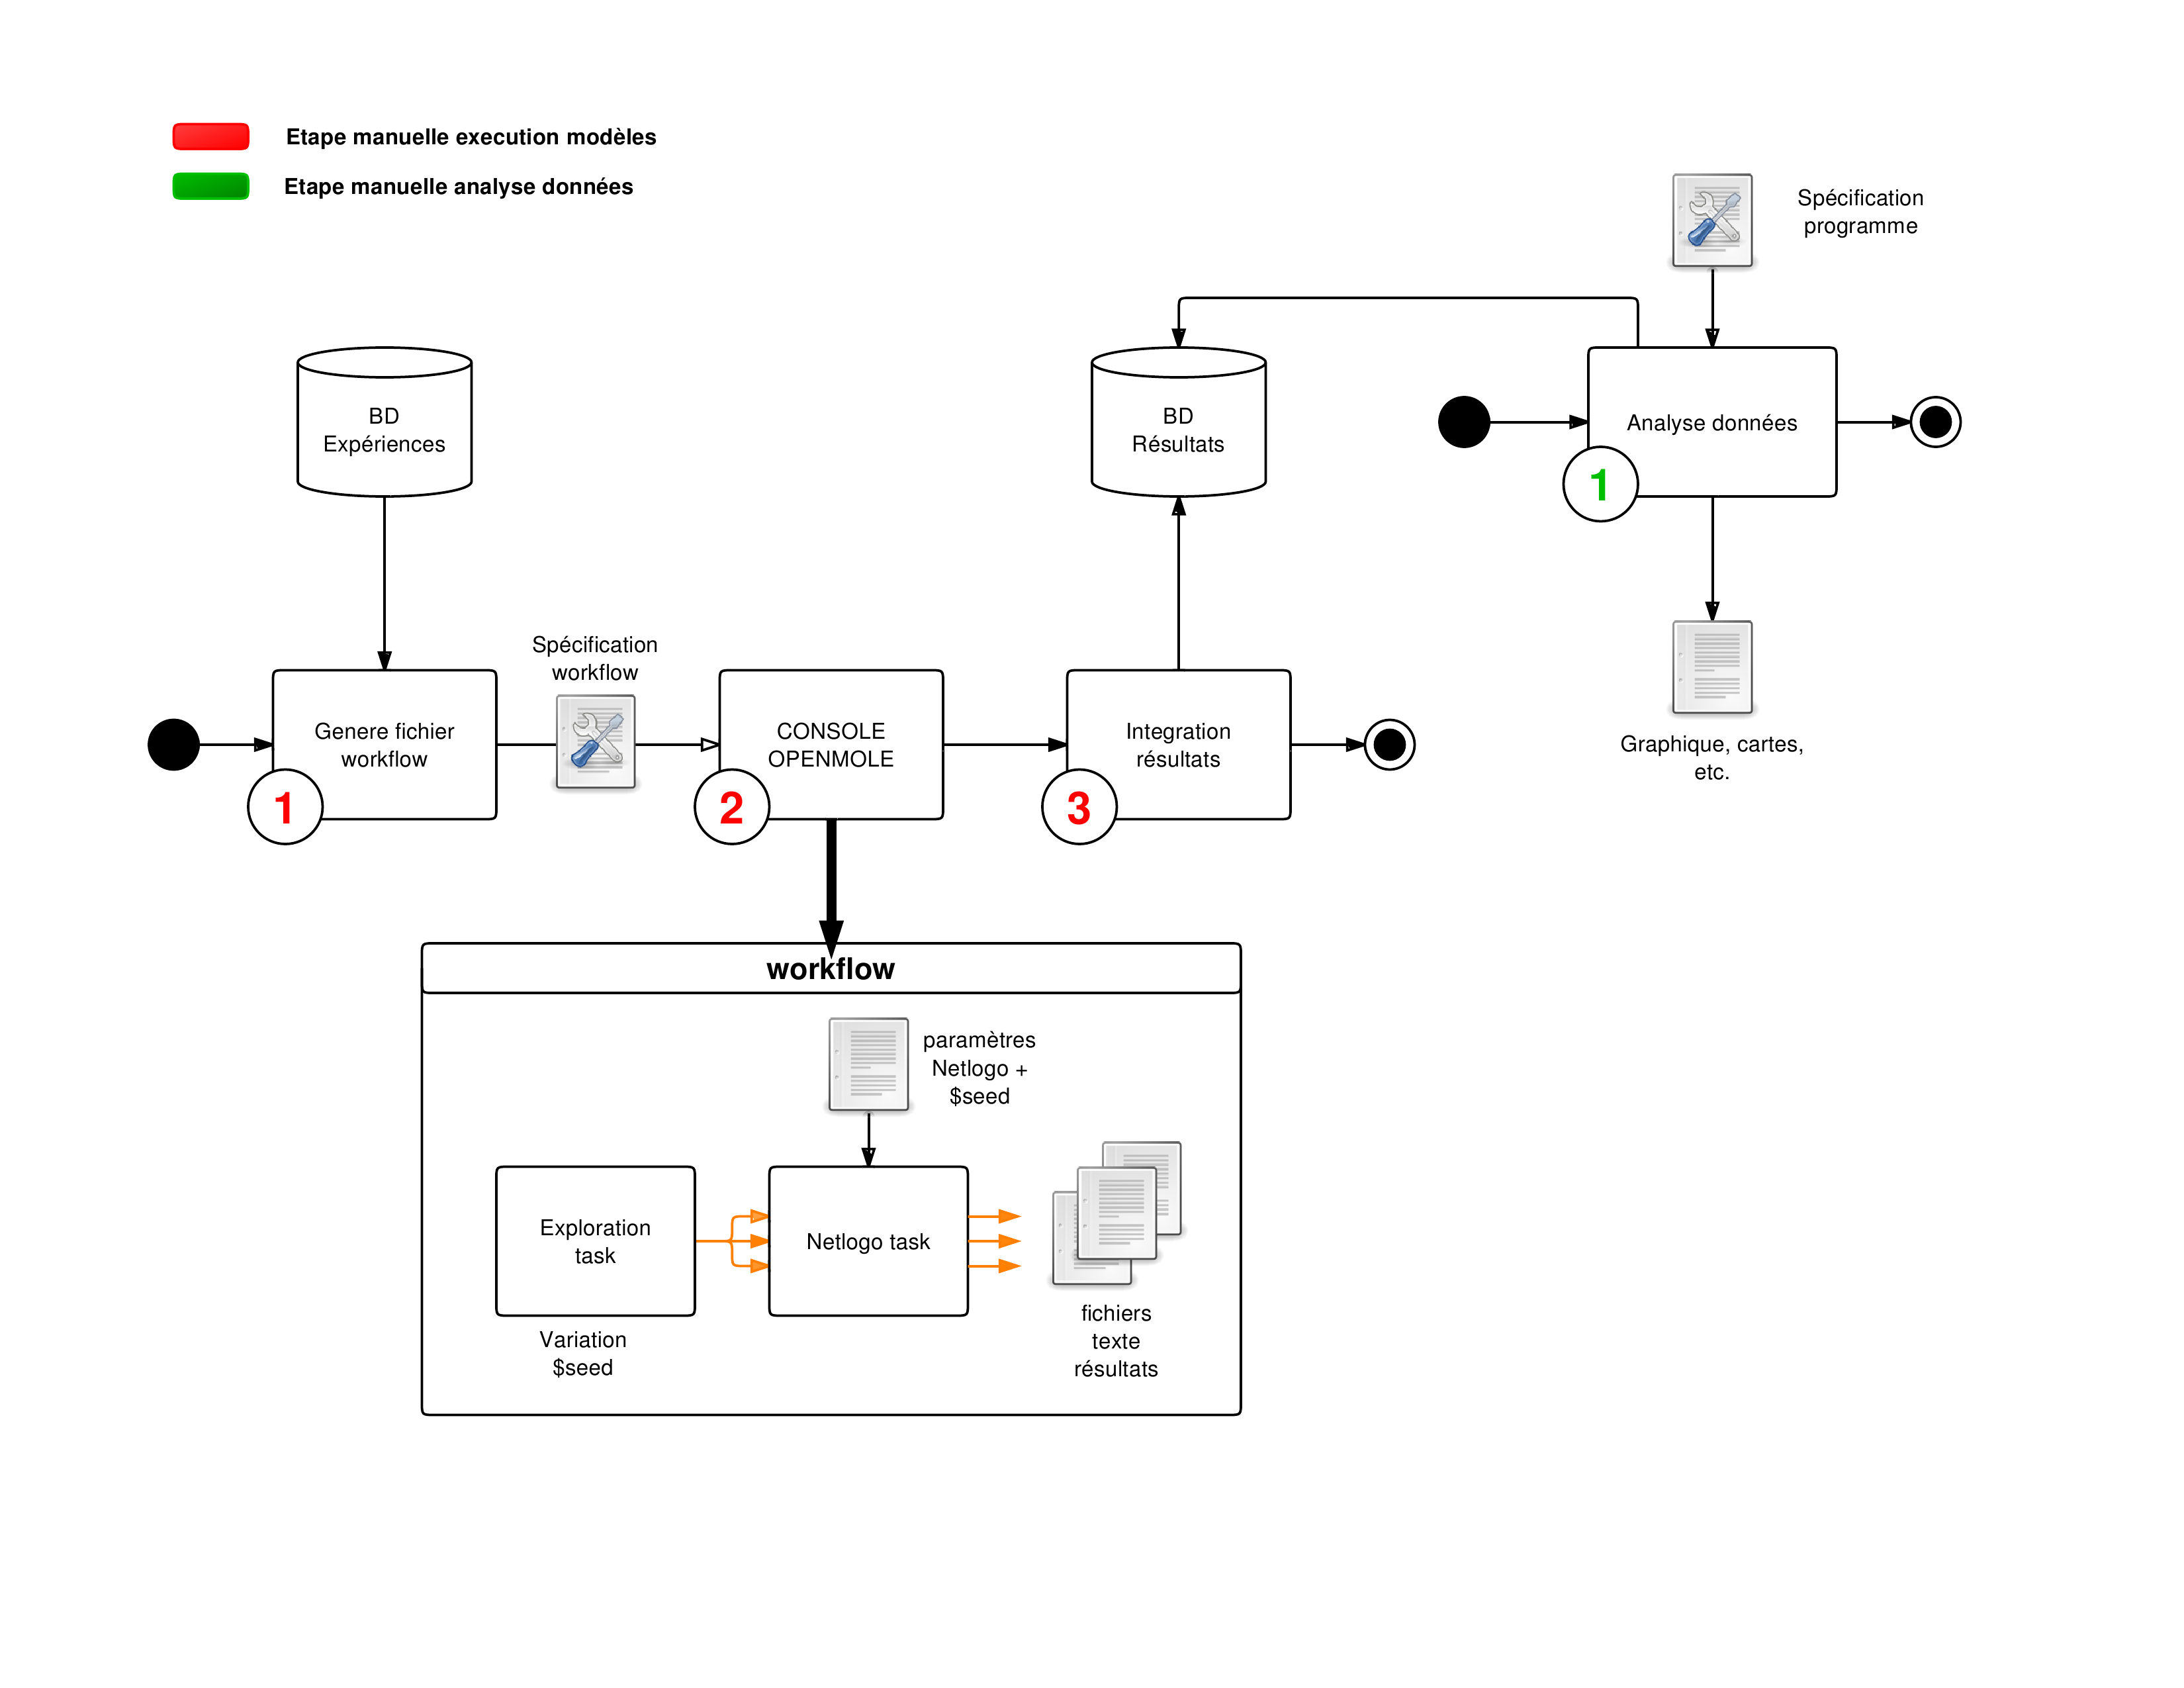
\includegraphics[width=1.0\linewidth]{oldplatform2.png}
 \end{sidecaption}
\end{figure}

La construction d'un logiciel interface devait permettre de piloter la construction et la sauvegarde des expérimentation, mais aussi la construction de rapport automatiques. Cela revient à construire un générateur de workflow capable d'envoyer les modèles de simulation sur grille de calcul et de stocker automatiquement une fois terminé ces résultats dans une base de données, exploitable de différentes façon : construction et consultation de rapport automatique pour un wiki, visualisation SIG, etc.

Au début de l'année 2011, juste après la première campagne de calibration du modèle SimpopLocal utilisant des algorithmes évolutionnaires (on y reviendra ensuite), il devient de plus en plus évident que non seulement l'intégration d'OpenMOLE dans une plateforme n'est pas possible, mais qu'en plus cette solution n'est pas viable, pour plusieurs raisons


- Le logiciel est encore en plein développement, il ne sera pas stable avant plusieurs mois, notamment le DSL permettant d'écrire les workflow.
- Les workflow ne peuvent pas être sauvegardé dans les premières version de la plateforme, mais c'est une priorité dans les développements en cours
- Deux ingénieurs à plein temps travaille dessus, alors que de mon coté je suis seul développeur à mi-temps entre le modèle de simulation SimpopLocal, la mise en oeuvre des explorations avec OpenMOLE, et la construction de la plateforme.
- Une bonne partie des outils déjà développé sont en Python ( génération de wf automatique, intégration des données dans une base, requetage de la base, construction des graphiques avec R et python,  etc.), alors que la plateforme OpenMOLE est en java/scala
- L'interface graphique pour la construction de workflow et de plan d'expérience interactif est développé par un ingénieur à plein temps, donc pourquoi redévelopper de mon coté un gestionnaire de plan d'expérience ?
- La coopération avec l'équipe d'OpenMOLE ne va qu'en se renforçant, et le maintient de deux projets indépendant partageant les mêmes idées n'a pas de sens

A cela il faut ajouter une autre évidence, les premières expériences pour l'exploration du modèle SimpopLocal produisent un volume de donnée déjà très important, ne serait-ce qu'à cause de la stochasticité, qui nécessite de nombreuses réplications du modèle (même jeu de valeur de paramètre, graine aléatoire différente). Ce n'est pas un problème technique, les bases de données mises en place à cette ocasion pouvant largement supporter un tel poids (quelques gigas), mais un problème méthodologique, a quoi cela sert-il de stocker un tel volume de données sur des simulations qui pour le moment ne sont pas calibré ? La fouille de données a posteriori est elle une si bonne idée dans ce cas précis ?

Prenons un exemple plus concret. Dans le cadre de SimpopLocal un des pattern recherché par les géographes correspond à une description de la hierarchisation du système à un temps $t$ final égal à 4000 pas de temps (1 pas de temps = 1 année), durée historique retenue par les experts. Dans une telle exploration a posteriori, la seule façon de qualifier si la reproduction de ce fait stylisé est correcte ou pas pour une simulation est de soumettre ce graphique pour évaluation à un expert. Si on réalise un plan complet sur les cinq paramètres retenu pour varier dans le modèle, avec une discrétisation uniforme en 10 valeurs, et une trentaine de réplications, cela représente vite quelques centaines de milliers d'execution du modèle pour cette seule expérimentation : $10^{5} * 30 = \num{300000}$. Admettons que l'on puisse résumer chaque ensemble de réplications dans un même graphique comportant la moyenne, la médiane, l'écart-type, etc. cela nous laisse quand même cent mille évaluation visuelles à réaliser manuellement. Sachant que l'on a aucune certitude sur la capacité de cette résolution de maille utilisé pour discrétiser l'espace de valeur de paramètre à detecter la zone de valeur de paramètre capable de reproduire ce fait stylisé.

On s'apercoit très vite que ce schéma d'expérimentation n'est pas viable pour calibrer un modèle, même simple, comme SimpopLocal. C'est un problème que nous avions déjà envisagé pour la plateforme avec Thomas Louail, la nécessité de pouvoir detecter automatiquement les \textit{patterns} recherchés en utilisant des algorithmes évolutionnaires, seulement à ce moment là, nous n'avions aucun outil fonctionnel à disposition, le stage de trois mois de A. Monzi pour développe une Interface aux algorithmes développés par B.Calvez n'ayant pas débouché sur un prototype utilisable sur Simpop2 \autocite[140-141]{Louail2010}

Un autre point important de convergence avec l'équipe d'ingénieurs d'OpenMOLE se présente alors, dans la possibilité d'utiliser des algorithmes évolutionnaires pour calibrer des simulations.

Plutôt que de réinventer la roue, pourquoi alors ne pas intégrer les outils qui manque aux géographes modélisateurs dans OpenMole, comme ce qui s'est déjà produit avec l'ajout de l'extension Netlogo.

- Ajouter des connecteurs en entrées / sorties vers les bases de données dans les workflows
- Ajouter une possibilité de visualiser des données géographiques dans la plateforme
- Ajouter la possibilité d'écrire ses propres scripts d'analyses statistiques dans la plateforme
- Réaliser un workflow utilisant des algorithmes génétiques Dans openMOLE.

A partir de là, les aspects plus géomatique prévu dans la plateforme initiale vont être mis entre parenthèse, pour se concentrer principalement sur la construction d'un prototype de méthodologie couplant SimpopLocal et OpenMOLE.




%SimpopLocal_h3_grille.nlogo qui tourne sur la grille en juin 2010, seule la seed est amené à varier pour le moment.


% Référence à Amblard Amblard2010 et Amblard2003 sur l'expérimentation au coeur du processus de modélisation.

% Partie Amblard a replacer sur SimExplorer.
\enquote{Le modélisateur doit donc se doter des méthodes et des outils particuliers de l’expérimentateur et les adapter à ses expériences virtuelles. Dans le cycle classique de modélisation construit sur un schéma analyse -> conception -> vérification -> tests (exploration) -> validation, nous nous concentrons donc sur la partie tests ou exploration, que nous cherchons à automatiser partiellement et à adapter aux modèles individus-centrés. Dans le cas d’un modèle individus-centré, nous considérons que l’exploration du modèle procède par approximations successives : les tests sont d’abord assez grossiers (maille large dans l’exploration des paramètres, niveau d’agrégation important dans les résultats) de manière à repérer les éléments les plus saillants de la dynamique, puis ces tests sont progressivement raffinés dans différentes directions identifiées aux étapes précédentes. L’ensemble de ces opérations peut s’avérer très long, et demander de répéter les expériences de nombreuses fois si les bons indicateurs agrégés n’ont pas été identifiés. Il est donc important d’optimiser ces explorations par le biais de plans d’expérience et de se doter d’outils permettant de faciliter leur définition, ainsi que la définition des variables agrégées résultats. C’est l’objectif de l’outil générique SimExplorer, actuellement en cours de développement, qui permettra la réalisation de plans d’expérience pour la simulation, de la manière la plus indépendante possible du noyau de simulation développé.}




Schéma présentation intégration OpenMOLE avec plateforme.

Protoslocal Forge mai 20111

\begin{framewithtitle}[geneseopenmole]{Genèse d'OpenMOLE}

A l'origine il y a le projet \textbf{SimExplorer} présenté dans la thèse de  Frédéric Amblard en 2003 \autocite{Amblard2003}. Cet outil expose déjà dans sa conception et son implémentation bien des idées qui seront reprise sans le savoir dans nos démarches. En effet, bien que cet outil soit cité dans cette publication de référence sur la validation pour le multi-agent en sciences humaines et sociales \autocite{Amblard2006}, de façon étrange, ce prototype ne trouvera pas écho auprès des géographes avant sa re-découverte en 2010, au travers d'un successeur en filiation directe, à savoir OpenMOLE.

La genèse de ce dernier est en effet lié à celle de SimExplorer. En décembre 2005 \textcite{Reuillon2008} commence le développement de DistMe pour son projet de thèse, un logiciel pour distribuer des réplication de simulation stochastique sur grille de calcul. David Hill (LIMOS) est le directeur de thèse de Romain Reuillon (UMR LIMOS Clermond), mais également le directeur de thèse de Frédéric Amblard (Cemagref) qui a déjà soutenu sa thèse en 2003. En 2007 environ, celui-ci conseille à Romain Reuillon de rencontrer l'équipe de Guillaume Defuant (CEMAGREF), situé sur le même campus, et qui travaille déjà depuis quelques années sur SimExplorer (Nicolas Dumoulin, Thierry Faure, Florent Schuffard). A ce moment là, Frédéric Amblard est déjà parti pour l'IRIT, Romain Reuillon ne l'ayant pas croisé.

L'équipe de Guillaume Defuant ainsi que Romain Reuillon, dépose un projet nommé Life Grid en 2008, financé par la région pour intégrer les travaux de DistMe dans SimExplorer. Une fois le projet accepté, Romain Reuillon travaille de janvier à novembre sur cette intégration, en coopération avec Florent Schuffard. Romain Reuillon démarre le 1 novembre 2008 à l'ISC PIF et soutient sa thèse le 28 novembre du même mois.

Un peu avant en 2007, l'ISC-PIF est alors sous la direction de son créateur Paul Bourgine. Avec David Chavalarias, ils décident d'achèter dans le cadre d'un partenariat avec les fonds de la région ile de france, un \textit{cluster} qui a pour but d'être mutualisé avec la grille de système complexe (700 000 euros) Toutefois, il y'a un différentiel entre cette vision mutualiste et le niveau technique des modélisateurs des systèmes complexes. Comme le dit Romain Reuillon, à l'époque \enquote{Personne ne savait s'en servir, c'est d'ailleurs comme ça que la possibilité d'un poste m'est arrivé aux oreilles, via les conseils de Guillaume Defuant, et une rencontre avec David Chavalarias, de passage au CEMAGREF-LISC de Clermond.}

Une fois en poste à l'ISC-PIF, Romain Reuillon propose à Paul Bourgine - au tournant de l'année 2008-2009 - de continuer à développer SimExplorer, qui deviendra environ un an plus tard un nouveau projet indépendant nommé OpenMOLE. Romain Reuillon veut en effet passer du système séquentiel de déroulement des tâches de SimExplorer, à un système de tâche indépendante présenté sous forme de \textit{workflow}. Les concepts étant déjà réfléchi depuis un certain temps, un premier prototype de workflow fonctionnel démontre la faisabilité des concepts quasiment un mois après le début du projet.

%Octobre 2010, tout openMOLE recodé en Scala.
Lors du passage de direction à Réné Doursat, Mathieu Leclaire est embauché en septembre 2009 sur un poste d'ingénieur grille spécifique à l'ISC (avec les crédits région de l'ISC-PIF). Il devient l'autre membre fondateur d'openMOLE, les deux continuant depuis à travailler à plein temps sur le logiciel.

\end{framewithtitle}


%A PLACER : L'exploration des modèles devient dès lors qu'on lui en donne l'occasion, le pilier central d'une réflexion qui semble rejaillir sur l'ensemble des développements, qu'il soit thématique, méthodologique, ou technique.  Il a donc fallu d'abord se déposséder de l'idée de plateforme pour l'évaluation des modèles tel que nous l'avions imaginé, pour la reconstruire à nouveau au travers d'un co-développement étroit avec des ingénieurs spécialisés dans le HPC. Une ressource informatique qui reste à ce jour le seul moyen d'explorer les modèles de simulation, et cela depuis les années 1980, date ou les géographes avaient déjà préssenti la nécessité d'un tel projet \ref{p:experience_minuit}. + Schéma

\paragraph{Quatrième moment, au delà du prototype}

 - de nouveaux projets
 - de nouvelles dynamiques
 - de nouvelles personnes


La première vient du fait que la thèse ici présenté co-évolue dans le temps et dans les thématiques abordés avec les réalisations d'une autre doctorante au laboratoire Géographie-Cités. Ainsi, c'est avec l'aide de Clara Schmitt, ingénieur agronome également titulaire d'un master 2 de Géographie, que nous allons travailler pendant plus d'une année et demi à la réalisation d'un modèle porteur des problématiques chères à la thèse de Clara Schmitt, sur lequel nous reviendrons également dans ce manuscrit.

C'est à peu près a ce moment là, et sous l'impulsion d'Arnaud Banos, alors président de l'Institut des Systèmes Complexes de Paris Ile-De-France, que va naître dans une nouvelle impulsion, une deuxième collaboration avec Romain Reuillon et Mathieu Leclaire, tout deux ingénieurs créateurs d'un logiciel développé dans l'objectif de répondre à des problématiques qui nous le verrons, viendront recouper directement des besoins précédemment évoqués pour l'exploration et l'analyse du modèle.


à fait favorable au changement des pratiques dans la construction et l'évaluation des modèles de simulation

% Résurgence de la problématique HPC.

--

Au détriment peut-être de constructions techniques, qui il faut bien le dire, dans un tel contexte d'inter-disciplinarité, sont éphémères.

Il faut s'imaginer sur quelles bases les outils ont été développés. Romain et Mathieu sont deux développeurs à plein temps sur un logiciel qui était jusqu'il y a peu encore en complète construction.

Dans ces conditions, vivre l'inter-disciplinarité c'est accepter d'un point de vue logiciel la construction d'une maison sur des sables mouvants. Vous vous arretez de soutenir la maison une semaine, un jour parfois, et la voilà à terre.

Les travaux qui paraissent en 2014, puis 2015 sont le fruit d'une inter-disciplinarité \textbf{vécue}, j'insiste sur ce dernier mot car on parle souvent plus d'inter-disciplinarité qu'on ne la pratique réellement, avec ses défis \autocite{Chapron2014} qui s'inscrit délibérement dans le mouvement \enquote{slow science}.


 2009 et 2010, l'objectif partait d'un certains nombre de frustration prenant racine  dans l'observation des limites des pratiques existantes dans le laboratoire et dans la littérature, pour évaluer les modèles existants, mais également les modèles en cours de construction.

  - celle de ne pas comprendre la dynamique de nos modèles, pourtant encore très simple
  - la constatation dans la littérature d'une certaine d'outils support des méthodes

  - très peu de réutilisabilité des comportements implémentés : vous vous trouver devant un choix d'implémentation, lequel sera le bon ?


Entre 2009 et 2010, deux rencontres

- Première rencontre avec Thomas Louail, Denise Pumain, Hélène Mathian, Léna Sanders autour de Simpop2

- Deuxième rencontre avec Arnaud Banos, Clara Schmitt

- Troisième rencontre avec Romain Reuillon, Mathieu Leclaire, Jeremy Figel


 ,  et illustre depuis bientot 4 ans un travail d'équipe tel qu'il peut s'établir au jour le jour, amenant avec lui ses forces et ces faiblesses. De par son articulation, tout l'enjeu de cette thèse sera je l'espère, de prouver, que oui, le total fait bien plus que la somme des parties.

Deux grandes collaboration viendront successivement marquer profondément la nature, l'avancement et le contenu de mes travaux.


Loin d'être nouvelle et teinté de maladresse, ces collaborations participent d'un processus qui s'inscrit et prolonge un mouvement historique, qui de ce fait évolue, et se renouvelle sans cesse depuis ces 30 40? dernières années au laboratoire Géographie-Cités (+ref ancien ?, ArcheoMedes, Transmondyn). Car c'est ainsi  au gré de rencontres interdisciplinaires parfois hasardés, mais le plus souvent recherchés, que se mêlent, se confrontent, s'exposent à la fois les expériences humaines et techniques.

Cet héritage disciplinaire solide fournit à notre étude un réseau, des pratiques, des théories, des outils  qui dans leur développement expriment à la fois partie de réponses tout autant que l'expression de leur propres limites. L'arrivée de nouvelles problématiques, quelles soient issues d'une reformulation ou d'un nouvel apport à la discipline, nous fournit une occasion supplémentaire de venir enrichir par l'apport de nouvelles méthodologies, de nouveaux outils, cet horizon toujours grandissant de pensées et de pratiques qui forment la communauté des systèmes complexes auquel nous appartenons.




--

Voici ce pour quoi openMOLE est un outils indispensable pour faire le liens entre les usages en SHS, et ces ressources distribués.

Les géographes francais utilisant actuellement la grille de calcul pour l'execution de simulation sont rattachés à la VO des système complexe européenne (\textit{vo.complex-systems.eu}), et sont principalement issue du laboratoire Géographie-Cités à Paris, et du laboratoire GEOLAB de Limoges.

Sans cette collaboration à la fois humaine et technique avec l'Institut des systèmes complexes de Paris (ISC-PIF), ce premier contact avec le \textit{Grid Computing} n'aurait probablement pas pu se faire.

% Cette plateforme peut elle faire autre chose ? Vais je pouvoir partager mon modele ou mon experience avec d'autres scientifiques ?

Dans un article daté de 2015, johnatan dursi
\href{http://www.dursi.ca/hpc-is-dying-and-mpi-is-killing-it/}{hpc is dying}

\subsection{Historique}

Evidemment il faut citer le travail important réalisé sur le prototype par Amblard, à la fois dans le démocratisation de la validation, mais également dans les outils.

\subsection{Principes et mise en oeuvre}

\section{Un nouveau framework pour systématiser l'évaluation des modèles de simulations : MGO}
\label{sec:MGO}

%%%%%%%%%%%%%%%%%%%%%%%%%%
%% NOTE CLEMENTINE
%%%%%%%%%%%%%%%%%%%%%%%%%%
% Je t'ai mis surtout des détails de forme dans le documents en pj parce que je suis incapable de juger le fond.
% Dans l'ensemble, tu avais l'air d'être inquiet de la lisibilité pour le néophyte, donc :
% - effectivement, c'est pas fastoche fastoche !
% - en fait je pense que là ou tu pourrais gagner en accessibilité (on va pas envisager le géographe des migrations en Afrique mais disons le quantitativiste moyen :), c'est sur le tout début.
% Au fur et à mesure de la lecture, on a tout les éléments on s'y retrouve et c'est intéressant et ça se lit bien.
% Par contre le début c'est chaud, et à mon avis pour deux raisons :
% - c'est la partie la plus théorique et on sent que même toi tu doutes un peu de l'intérêt de classifier les algo alors on est pas convaincu non plus et on sait pas ou ça va nous mener.
% - je pense qu'il faut que tu annonces beaucoup plus tôt, plus fort et plus souvent à quoi ça sert qu'on s'intéresse aux métaheuristiques, aux espaces de résultats et aux fronts de Pareto. Pour ne pas avoir à tout réorganiser, tu peux surement tester ce que ça donne de présenter dès le début le besoin d'algo evolutionaire en simulation géo. et comme ça on apprend plein de trucs par la suite, mais on voit ou tu nous emmènes et comment on fait notre choix parmi toutes les solutions que tu présentes...

%%et pourquoi ne pas utiliser les modèles au début pour annoncer les problèmes de modélisation et les enjeux de calibration?

%%%%%%%%%%%%%%%%%%%%%%

% Présentation de l'interet de ces techniques
% A priori déjà présenté ailleurs ?
%\subsubsection{Quelle utilité pour la construction et l'évaluation de modèle de simulation ?}

%Le chapitre 1 se terminait déjà sur la difficulté pour calibrer les modèles. Le chapitre 2 a prouvé que la construction et l'évaluation d'un modèle était deux processus indissociables,


% Fil plus chronologique, guidé par les besoins !

% - Accéder au HPC et Grid Computing
%

% - Présentation modèles exemples
% - OpenMOLE
% - MGO
%
% Plan temporaire MGO :
% - Présentation besoins / objectifs.
% - Insufisance EC existant (2.2.3.1 actuel)
% - Présentation plus large de la discipline + encadré resituant SLocal
% - Mise en oeuvre MGO
%	- Historique
%   - Principe conception innovant
% - Mise en oeuvre couplage MGO - openMOLE
% - Premier prototype, bilan autour de l'expérience SLocal

% Prise de recul sur la méthodologie, accointance et critique de la méthode POM avancé par Grimm ?

\subsection{Présentation des modèles utilisés}

Le choix est fait dans cette section de faire appel à la fois un modèle jouet (pour la compréhension générale), mais également un modèle réel (pour montrer que cela marche).

\subsubsection{un modèle jouet sur les fourmis}

Le modèle de simulation \textbf{Ants} est une reproduction par \textcite{Wilensky1997} d'un modèle originellement en StarLogo en Netlogo. Celui-ci est disponible sur le \href{http://ccl.northwestern.edu/netlogo/models/Ants}{@site} de Netlogo, et par défaut dans la bibliothèque de modèle du logiciel.

\begin{figure}[H]
		\centering
	 	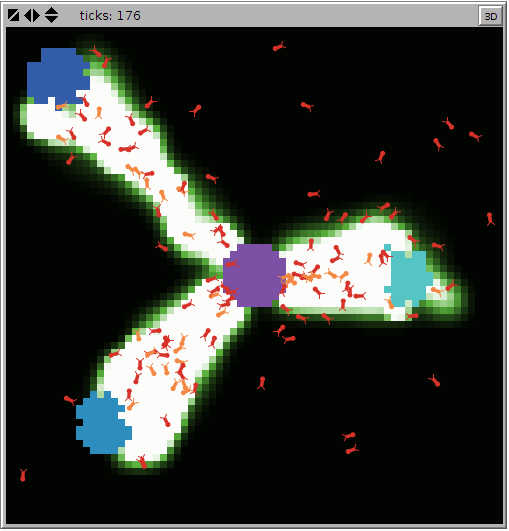
\includegraphics[width=.6\linewidth]{ants.png}
\end{figure}

Dans ce modèle Netlogo, une colonie de fourmis fourrage à la recherche de nourriture. Chaque fourmi suit un ensemble de règles simple, mais la colonie prise dans son ensemble réagit de façon complexe. Quand une fourmis trouve un morceau de nourriture, elle ramène celle-ci dans son nid, en laissant une empreinte chimique derrière elle. Lorsque les autres fourmis renifle cette trace, elle suive la piste jusqu'à la nourriture. Plus le nombre de fourmis rapportant de la nourriture vient à augmenter, plus la piste chimique est renforcé par leur passage.

Ce modèle est constitué de trois paramètres :
\begin{itemize}[label=\textbullet,noitemsep,nolistsep]
\item Une $Population$ de fourmis initiale
\item Un taux $Evaporation-rate$ qui controle l'évaporation de la trace chimique
\item un taux $Diffusion-rate$ qui controle la diffusion de la trace chimique
\end{itemize}

\subsubsection{un modèle de simulation appliqué SimpopLocal}

Seul un résumé du projet SimpopLocal sera présenté ici, car la présentation détaillé du modèle, les problématiques qui ont motivés sa construction et son exploration, ainsi que les résultats, ont déjà fait l'objet d'une présentation détaillé à la fois dans un article EPB paru en 2015 \autocite{Schmitt2015} (joint en annexe) , un article paru dans JASSS en 2015 \autocite{Reuillon2015}, mais également dans plusieurs chapitres de thèse \autocite{Schmitt2014}.

Bien que les travaux autour de ce modèle de simulation puissent apparaitre comme nominatif - du fait entre autre qu'il faille bien inscrire à un moment donné ou un autre ces travaux dans une thèse - je tiens toutefois à repréciser qu'il s'agit à mon sens d'un travail partagé, ou rien n'aurait été possible sans la participation de l'un ou l'autre des collaborateurs, que cela soit dans la construction des modèles ou de certains graphiques, dans l'exploration des modèles, dans l'analyse des résultats, etc. Comme on pouvait s'y attendre compte tenu de la multiplicité de compétences nécessaire pour une telle construction, les réalisations des acteurs sont améliorés et/ou contraintes par une forme plus ou moins forte d'inter-dépendance propre à cette inter-disciplinarité \autocite{Chapron2014}.

Le modèle SimpopLocal a également subi de nombreux redéveloppements, que cela soit dans sa version Netlogo (janvier 2010), Scala (avril 2012), et enfin dans son intégration dans SimPuzzle (avril 2013). En dehors des quelques évolutions de syntaxe, les \textit{workflow} utilisés pour explorer ce modèle sont quasi-similaires et cela quelque soit la version utilisée, ce qui constitue déjà en soit  une preuve de robustesse de la plateforme utilisé.



%Le \textit{framework} MGO (Multi Goal Optimization)

\subsection{Le domaine des algorithmes métaheuristiques, une sous-discipline de l'Optimisation}

\begin{figure}[h]
\begin{sidecaption}[fortoc]{ Vue d'ensemble des algorithmes d'optimisation repris de l'état de l'art très complet de \textcite[32]{Weise2011}}[fig:S_OverviewOptimisation]
  \centering
 
\includegraphics[width=.9\linewidth]{overview_optimisation_algorithm.png}
  \end{sidecaption}
\end{figure}

Pour mieux comprendre par la suite quelle est la spécificitée des algorithmes evolutionnaires (\textit{Evolutionary Algorithms} ou EA), il est nécessaire de donner quelques éléments de contexte et de définitions plus généraux concernant la branche d'étude dans lequel ceux-ci se situent. Il faut par ailleurs mettre en garde le lecteur que la plupart des définitions et des analyses présentés ici sont inspirés ou extraits d'ouvrages de synthèses à destination d'un public très large \autocites{Weise2011, Luke2013, Brownlee2012}. Par conséquent il faut garder à l'esprit que plusieurs de ces termes peuvent être discutés, enrichis, critiqués ou prendre des sens différents dans chacune des sous branche (voir figure \ref{fig:S_OverviewOptimisation}) que compte ce domaine très général qu'est l'optimisation.

\subsubsection{Q'est ce que l'optimisation ?}
\label{sssec:Optimisation}

Pour \textcite[22]{Weise2011}, l'optimisation \foreignquote{english}{ [...] is the process of solving an optimization problem, i. e., finding suitable solutions for it}, un problème d'optimisation nécessitant de trouver \foreignquote{english}{ [...] an input value $x^*$ for which a mathematical function $f$ takes on the smallest possible value (while usually obeying to some restrictions on the possible values of $x^*$ )}, la notation mathématique astérisque $^*$ désignant ici une valeur optimale.

Sortie de cette définition mathématique, l'optimisation peut également se définir par la mise en oeuvre d'algorithmes spécifiques. La littérature informatique met à disposition des programmeurs un ensemble d'algorithmes capables de fournir des solutions exactes dans un temps fini à un certain nombre de problèmes bien définis. C'est le cas par exemple des nombreux algorithmes de tri. Une autre classe d'algorithmes (\textit{optimization algorithms}) peut être employée lorsqu'il n'existe pas d'algorithme dédié (\textit{dedicated algorithms}), soit parce que le problème est trop spécifique, soit parce que personne n'a trouvé de solution efficace pour résoudre ce problème.

Dans ce cadre, le terme d'optimisation globale \foreignquote{english}{ [...] is optimization with the goal of finding solutions $x^*$ for a given optimization problem which have the property that no other, better solutions exist.} Le terme \enquote{global} nécessite à la différence d'une recherche qui serait \enquote{locale}, de se concentrer sur l'obtention souvent plus couteuse et plus complexe d'un optimum global, minimum ou maximum, dominant par sa qualité l'ensemble des valeurs recherchées en entrée de la fonction à optimiser.

Bien que souvent beaucoup plus lent, moins précis, et plus consommateurs de ressources que les algorithmes dédiés, ces algorithmes d'optimisations nécessitent aussi beaucoup moins d'informations pour pouvoir être executés : \foreignquote{english}{Most often, these algorithms only need a definition of the structure of possible solutions and a function $f$ which tells measures the quality of a candidate solution. Based on this information, they try to find solutions for which $f$ takes on the best values.} \autocite[24]{Weise2011}

Ces algorithmes s'appuient donc sur différents types de stratégies pour tirer parti du peu d'information obtenue via cette fonction $f$. De nature très diverse, on retient pour séparer une première fois ces stratégies une typologie en deux classes.

\begin{itemize}[label=\textbullet]
\litem{\textit{Probabilistic Approaches}} Les approches stochastiques désignées dans la fig. \ref{fig:S_OverviewOptimisation} sont capables de trouver un optimum assez rapidement, mais ne peuvent pas en garantir la propriété \enquote{globale}
\litem{\textit{Deterministic Approaches}} Les approches déterministes également désignées dans la fig. \ref{fig:S_OverviewOptimisation} peuvent certes garantir au moins théoriquement l'obtention d'un optimum global, mais s'éxecutent souvent au détriment d'un coût computationnel elevé.
\end{itemize}

Ces deux approches partagent également des difficultés communes, et découvrent leurs limites à des degrés divers en fonction des stratégies mise en oeuvre, dès lors que l'espace de recherche à parcourir devient trop important.

C'est le cas par exemple de l'espace de recherche de toute une sous-catégorie de problèmes \textit{NP-Complet} \Anote{np_complet_def} d'optimisation combinatoire \textit{Combinatorial Optimization Problems} (COP). Ce domaine contient par exemple les problèmes bien connus du voyageur de commerce \textit{Travelling salesman problem} (TSP), ou encore le problème du sac à dos \textit{Knapsack Problem} (KP) \Anote{note_knapsack}. Avec l'augmentation du nombre d'éléments entrant dans la définition de ces problèmes, il devient impossible de passer en revue l'ensemble des combinaisons (solutions possibles). Ce qui a pour conséquence de rendre difficile tout autant la découverte d'un optimum global, que la mesure de qualité de celui-ci, car pour établir cette dernière il nous faudrait logiquement connaitre la solution optimale, or c'est cela même que nous cherchons.

Cette première typologie recoupe une autre propriété des algorithmes. La littérature informatique qualifie ainsi d'\textit{exacts} les algorithmes dont l'exécution garantit un résultat optimum à coup sûr, d'\textit{approximate algorithms} les algorithmes capables de donner une mesure proche d'un optimum sans pouvoir en garantir la qualité, et d'\textit{approximation algorithms} les algorithmes capables de donner une mesure proche d'un optimum assortie d'une preuve de qualité. Cette dernière classe n'est pas à confondre avec une classe d'algorithmes cherchant à conserver l'optimalité en limitant par diverses stratégies le coût temporel de résolution, mais bien l'inverse, relâcher la contrainte d'optimalité, mais aussi peu que possible. Les \textit{approximations algorithms} sont une donc une sous classe d'\textit{approximate algorithms}, et constituent une branche d'étude à eux seuls, car même dans le cas de problèmes \textit{NP-Complet}, ils offrent dans des dimensions raisonnables et propres à chacun des problèmes une solution sub-optimale d'erreur mesurable et donc potentiellement améliorable, voire comparable, notamment avec les résultats donnés de façon non analytique par d'autre stratégies.
%http://en.wikipedia.org/wiki/Approximation_algorithm#cite_ref-kann92onthe_3-4

On retrouve parfois rangé \enquote{en vrac} dans la classe des \textit{approximate algorithms} la classe des heuristiques et métaheuristiques, deux termes définis plus en détail dans la section suivante.

%On nomme métaheuristique (\textit{metaheuristic}) ce type d'algorithmes s'appuyant sur des heuristiques (\textit{heuristic}).

\subsubsection{Quelle définition peut on donner pour une heuristique (\textit{heuristic}) ? }
\label{sssec:heuristique}

Le terme heuristique \textit{heuristic} vient du Grec \textit{heuriskein} que l'on peut traduire par \foreignquote{english}{to find}, ou \foreignquote{english}{to discover}. D'usage plus large que dans la simple discipline informatique, nous retiendrons ici ce terme seulement sous son sens spécifique contextuel à l'optimisation. Rattaché à la définition d'un problème (\textit{problem dependent}), on définit une heuristique comme une mesure approximative pour définir la qualité d'une solution candidate \autocite[34]{Weise2011}.

%http://stackoverflow.com/questions/9140860/heuristic-function-for-finding-the-path-using-a-star
%http://stackoverflow.com/questions/9140860/heuristic-function-for-finding-the-path-using-a-star
%http://stackoverflow.com/questions/11779589/connection-between-a-star-search-and-integer-programming-extending-a-star
Si on se penche sur la classe d'algorithmes dédiés au problème de recherche du plus court chemin, les heuristiques sont souvent utilisées en appui des algorithmes de parcours de graphe, soit pour converger plus rapidement vers une solution optimale, soit pour justement se libérer de cette contrainte d'optimalité en visant un gain de temps au détriment de la précision. Si on prend par exemple l'algorithme de Djikstra, celui-ci n'utilise pas d'heuristique et garantit que le plus court chemin résultant sera optimal, car tous les chemins possibles entre le point de départ $A$ et le point final $B$ auront été analysés par celui-ci. Il est néanmoins connu comme étant très coûteux d'utilisation dès que le graphe dépasse un certain nombre de noeuds. L'algorithme déterministe $A^*$ s'appuie par contre sur une fonction heuristique $h(n)$ (une estimation du coût minimal reliant le noeud $n$ au noeud final) pour guider l'algorithme dans le processus incrémental de sélection d'un prochain noeud constitutif d'un chemin. En jouant sur cette heuristique, on est ainsi capable de déterminer si l'algorithme doit mettre la priorité sur la vitesse ou la précision, $h(0)$ étant équivalent ici à l'algorithme de Djikstra. Si l'heuristique est bien choisie (on dit ici que l'heuristique est admissible), alors $A^*$ garanti aussi l'optimalité du chemin trouvé, avec à la clef un coût computationnel moindre, car seule une partie des noeuds de l'ensemble du graphe auront été explorés par l'algorithme. Une autre heuristique misant plus sur la vitesse d'exécution pourra définir un chemin cette fois-ci sub-optimal avec un coût computationnel encore plus réduit. Il est à noter ici que l'utilisation d'une heuristique dans un programme n'est pas forcément motivée par la recherche d'un optimum global, mais par le gain de temps. Ainsi, un utilisateur peut très bien avoir les moyens d'obtenir un chemin optimal (Djikstra) sur une petite combinatoire de noeuds, mais peut vouloir prendre un raccourci en utilisant une méthode moins couteuse ($A^*$). Un scénario très souvent mis en avant dans la programmation de jeux sur ordinateur, où l'on cherche régulièrement à gagner du temps, tout en se rapprochant d'un comportement faillible imitant plus un adversaire de type humain.

La forme prise par une heuristique est variable, et peut aller comme vu ci-dessus avec l'exemple $A^*$ d'une simple fonction mathématique de coût intégrée à un algorithme classique de parcours de graphes, à un algorithme beaucoup plus complexe intégrant de multiples prises de décisions pour estimer ce même coût. Dans le livre \textit{Code Complete} de \textcite[12]{McConnell2004}, celui-ci donne un exemple assez parlant pour illustrer la subtile différence qui sépare la description d'un algorithme employé au sens courant pour désigner un algorithme déterministe exact fournissant à coup sûr une solution, et la description d'un algorithme déterministe ou stochastique heuristique (ou appuyé par une heuristique) fournissant seulement un guide pour trouver, éventuellement, une solution.

\foreignquote{english}{Here's an algorithm for driving to someone's house: Take Highway's 167 south to Puyallup. Take the South Hill Mall exit and drive 4.5 miles up the hill. Turn right at the light by the grocery store, and then take the first left. Turn into the driveaway of the large tan house on the left, at 714 North Cedar}

\foreignquote{english}{Here's an heuristic for getting to someone's house: Find the last letter we mailed you. Drive to the town in the return adress. When you get to town, ask someone where our house is. Everyone knows us - someone will be glad to help you. If you can't find anyone, call us from a public phone, and we'll come get you.}

Il faut toutefois éviter de considérer les heuristiques comme appartenant à la seule classe des \textit{approximate algorithms}, car le terme ne se laisse pas facilement enfermer dans une typologie trop simple. En effet de multiples problèmes trouvent une solution exacte jusqu'à un certain niveau de complexification, à partir duquel on fait généralement appel aux heuristiques, soit par un appel à d'autres méthodes intégrant des heuristiques, soit par une intégration d'heuristiques aux méthodes existantes. Ainsi de nombreuses classes d'heuristiques sont utilisées de façon transversale, et apparaissent donc aussi comme composantes manipulées dans la classes des \textit{approximation algorithms}. L'heuristique gloutonne \textit{greedy algorithm} \Anote{greedy_description} apparaît de façon transversale à la fois comme une solution d'approximation pour le \textit{Knapsack Problem} (KP) mais également comme moteur dans le cadre d'algorithmes déterministes exacts comme la recherche du plus court chemin de Djikstra. Un autre algorithme nommé \textit{A*} (\textit{A-Star}) qui englobe Djikstra comme cas particulier, est quant à lui capable de fournir tout à la fois une mesure exacte ou approximée en fonction de l'heuristique injectée et du niveau de complexité du problème abordé.

\subsubsection{Quelle définition peut on donner pour une métaheuristique (\textit{metaheuristic}) ?}
\label{sssec:metaheuristique}

Le terme métaheuristique est d'origine plus moderne \autocite{Glover1986}, et a permis d'englober a posteriori des algorithmes jusque là qualifiés d'heuristiques. C'est le cas par exemple d'une bonne partie des algorithmes évolutionnaires, qui émergent principalement au cours des années 1960-1970. Cette remarque d'ordre historique est à l'origine d'une première ambiguité entre les termes auquelle il faut encore ajouter les inquiétudes exprimées par \textcite{Luke2013}. Pour ce dernier, le terme métaheuristique est en réalité plutôt malheureux pour définir cette catégorie d'algorithmes, car contrairement à ce que laisse entendre ce terme, \textit{une heuristique pour ou à propos d'une heuristique}, ce n'est pas de cela dont il s'agit ici.

Voici comment \textcite[8]{Brownlee2012} perçoit la différence entre les deux termes : \foreignquote{english}{Like heuristics, metaheuristics may be considered a general algorithmic framework that can be applied to different optimization problems with relative few modifications to adapt them to a specific problem. The difference is that metaheuristics are intended to extend the capabilities of heuristics by combining one or more heuristic methods (referred to as procedures) using a higher-level strategy (hence ‘meta’). A procedure in a metaheuristic is considered black-box in that little (if any) prior knowledge is known about it by the metaheuristic, and as such it may be replaced with a different procedure. Procedures may be as simple as the manipulation of a representation, or as complex as another complete metaheuristic. Some examples of metaheuristics include iterated local search, tabu search, the genetic algorithm, ant colony optimization, and simulated annealing.}

Le terme \enquote{méta-} renvoie plus en définitive au concept générique de \enquote{stratégie de recherche} prenant la forme d'un algorithme d'optimisation capable de mélanger, manipuler des heuristiques ou d'autres métaheuristiques (cf. points \ref{enum_meta_a} et \ref{enum_meta_h}) \Anote{def_meta_weise}. Contrairement aux heuristiques, les métaheuristiques se définissent plus comme un système fait de composants, dont la plasticité permet le support et l'interaction nécessaire au développement d'heuristiques plus ciblées (\textit{problem dependent}) \Anote{def_meta_sorensen}. La structure offre un patron d'usage initial (\textit{pattern}) qui reste indépendant du problème abordé (\textit{problem independent}) (cf. \ref{enum_meta_g}), tout en restant évolutif, comme le montre le fort développement de cette discipline depuis les années 1980. Ce principe de flexibilité, on le retrouve par exemple dans la classe des EC, comme le mettent bien en valeur Bach, Hammel et Schwefel en 1997, dans une publication introduisant l'EC dans la série renommée des \textit{IEEE Transactions} :

\foreignquote{english}{We argue that the most significant advantage of using evolutionary search lies in the gain of exibility and adaptability to the task at hand, in combination with robust performance (although this depends on the problem class) and global search characteristics. In fact, evolutionary computation should be understood as a general adaptable concept for problem solving, especially well suited for solving difficult optimization problems, rather than a collection of related and ready-to-use algorithms. The majority of current implementations of evolutionary algorithms descend from three strongly related but independently developed approaches: genetic algorithms,evolutionary programming , and evolution strategies. [...] The fundamental difference in the evolutionary computation approach is to adapt the method to the problem at hand. In our opinion, evolutionary algorithms should not be considered as off-the-peg, ready-to-use algorithms but rather as a general concept which can be tailored to most of the real-world applications that often are beyond solution by means of traditional methods. Once a successful EC-framework has been developed it can be incrementally adapted to the problem under consideration, to changes of the requirements of the project, to modifications of the model and to the change of hardware resources.} \autocite{Back1997a}

Enfin, toujours dans une tentative de positionner ce terme dans une typologie, il faut savoir qu'une classification trop rapide de ces méthodes dans les seuls \textit{approximate algorithms} peut également être critiqué. Si les méthodes métaheuristiques sont effectivement souvent connues pour ne pas avancer de preuve, des travaux récents montrent toutefois qu'il existe de nouveaux algorithmes permettant de garantir dans certaines conditions un optimum global (CP-Algorithm de \autocite{Reuillon2015}). Tout dépend donc du degré et de la nature que l'on veut bien associer à la notion d'\textit{approximation} lorsqu'il s'agit de fournir une mesure d'éloignement de l'optimum. Les \textit{approximation algorithms} semblent toutefois plus intéressés par l'établissement d'une preuve au sens mathématique, et se concentrent avant tout sur un ensemble relativement limité de problèmes d'optimisation discret, ce qui ne semble pas être le but des métaheuristiques dans les deux cas. \autocites[1-6]{Kann1992}[13-15]{Williamson2011} %Metaheuristics: From Design to Implementation Par El-Ghazali Talbi

%You could think of a heuristic like an approximate (not approximation) solution to a problem. The difference between approximate and approximation is that the first is about getting a good guess of the solution of a problem, but that you don't really know how good it is. The second is about getting a solution for which you can prove how close it is to the optimal solution.

Enfin bien d'autres sous classifications sont possibles prenant plus ou moins en compte les spécificités propres aux différents algorithmes, comme celle opposant par exemple les stratégies utilisées en interne pour parcourir l'espace de recherche (generationel contre \textit{steady-state}, ou individuel contre populationel), la dimensionnalité possible pour la résolution des problèmes (mono-objectif contre multi-objectif), l'inspiration d'origine (naturelle biologique contre inspirations autres), etc.

Toute classification monocritère est donc rendue très difficile, une voie s'étant même ouverte pour tenter de classer ces algorithmes suivant la nature et le niveau d'opération de ces hybridations. L'origine de cette difficulté tient dans une pratique courante et assumée d'hybridation entre les différentes techniques afin de réunir le meilleur de chacune d'elles au sein de nouvelle proposition de recherche. De fait, il est important pour la suite de cerner au mieux la classe d'algorithme d'optimisation que nous allons aborder, et de définir pourquoi nous l'avons abordé. Nous nous intéresserons principalement dans la suite de cette présentation aux approches stochastiques métaheuristiques inspirées par la métaphore biologique, nommée \textit{Evolutionary Computation} (EC) ( voir figure \ref{fig:S_OverviewOptimisation}). La section \ref{xx} permettra de dégager les spécificités de cette subdivision, mais en attendant il nous faut d'abord présenter les principaux termes et concepts communs à cette classe d'algorithmes d'optimisation.

Devant la difficulté d'établissement d'une définition englobante, plusieurs auteurs semblent s'accorder pour faire du rattachement d'un algorithme à cette catégorie, une correspondance plus ou moins lâche avec un ensemble de propriétés généralement observées. En évitant une définition trop vague ou trop restrictive, on espère ainsi récupérer dans cette classe certains hybrides intéressants.

Voici un exemple de propriétés issues de \textcite{Blum2003} et traduites ci dessous :

%label=$\blacktriangleright$
\begin{enumerate}[label=(\alph*),labelindent=\parindent,leftmargin=*]
	\item Les métaheuristiques sont des stratégies qui \enquote{guident} le processus de recherche. \label{enum_meta_a}
	\item Leur objectif est d'explorer l'espace de recherche efficacement pour trouver les solutions quasi-optimales. \label{enum_meta_b}
	\item L'étendue des techniques que constitue la classe des algorithmes métaheuristiques va de la simple recherche locale à un processus d'apprentissage complexe. \label{enum_meta_c}
	\item Les algorithmes métaheuristiques sont approximatifs et la plupart du temps non déterministes. \label{enum_meta_d}
	\item Les métaheuristiques peuvent incorporer des mécanismes pour éviter d'être piégé dans une portion confinée de l'espace de recherche. \label{enum_meta_e}
	\item Les concepts de bases des métaheuristiques permettent d'adopter un certain degré d'abstraction dans la description. \label{enum_meta_f}
	\item Les métaheuristiques ne sont pas \textit{problem-specific}. \label{enum_meta_g}
	\item Les métaheuristiques peuvent faire usage d'une expertise du domaine au travers des heuristiques controlées par une stratégie de plus haut niveau. \label{enum_meta_h}
	\item La plupart des métaheuristiques actuelles font appel à une mémoire pour améliorer le processus qui guide la recherche. \label{enum_meta_i}
\end{enumerate}

Afin de mieux comprendre cette table de propriétés un peu abstraite, il est proposé de reprendre ces différents points au travers d'une lecture commentée, en commencant par une question ciblé sur la mécanique interne régissant ce type de technique.

\textit{Comment se matérialise la recherche de solutions optimisées dans une métaheuristique ?}

Si on considère les problèmes de combinatoires discrets comme \textit{TSP} ou \textit{Knapsack}, on a déjà vu que le nombre de combinaisons à évaluer lors d'une augmentation du nombre d'éléments participant à la définition du problème devient très vite problématique si on cherche à trouver une solution optimale exacte. Si on prend le cas d'un exemple plus ludique d'optimisations discrètes dans la branche des jeux (\textit{Combinatorial game theory}), le nombre de combinaisons légales possibles pour un plateau de 19 par 19 dans le jeu de GO chinois est estimé par \textcite{Tromp2007} à $2.08168199382×10^{170}$ . Même si certains auteurs comme Tromp estime qu'un tel calcul sera possible d'ici quelques mois \Anote{tromp_appel_calcul}, les problématiques posés par ce jeu mettent au défi les meilleurs programmes en intelligence artificielle \autocite{Bouzi2001}, et cela malgré des progrès spectaculaires ces dernières années, via notamment l'utilisation d'heuristique plus efficace que les approches classiques \Anote{mcts_go}.  Dans le cas d'un problème continu discrétisé, comme la recherche des meilleures valeurs de paramètres pour une simulation, la mise en oeuvre d'un plan factoriel complet (d'autres types de stratégies beaucoup plus fines existent) pose un problème double.

\hl{Correction orthographe à faire}
D'une part ce choix ne résout en rien la problématique combinatoire. Donnons un exemple plus concret, si une simulation possède 5 paramètres, chacun de ces paramètres étant discrétisé en 10 pas, cela nous donne déjà $10^5$ combinaisons possibles à évaluer. Si on considère que le modèle de simulation ainsi exécuté est stochastique (10 réplications), dans un délai relativement rapide (1 minute), la durée totale d'exécution de ce plan, pourtant relativement \enquote{grossier} d'un point de vue de la couverture de l'espace des paramètres, est environ égale à 2 années de calcul... La parallélisation d'un tel calcul, c'est-à-dire son execution sur plusieurs processeurs ou ordinateurs en parallèle, pourrait évidemment réduire ce temps de calcul à des dimensions plus raisonnables, mais c'est sans compter sur un deuxième problème, plus contraignant.

\begin{figure}[htbp]
	\begin{sidecaption}[fortoc]{Illustration des effets de la \textit{Curse Dimensionality} sur un plan d'expérience de 9 points entre 0 et 1 exclus. }[fig:curse]
	 \centering
	 	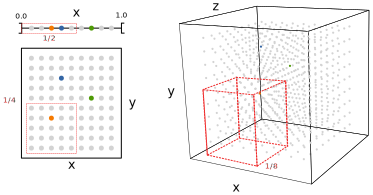
\includegraphics[width=.9\linewidth]{plot3d.pdf}
	\end{sidecaption}
\end{figure}

Avec le choix d'une telle maille pour la discrétisation des paramètres, c'est prendre le risque de passer à côté de solutions potentielles, une problématique contraignante d'autant plus qu'elle se complexifie avec l'augmentation du nombre de paramètres, comme le dicte le phénomène de \textit{Curse Dimensionality} établit par Richard Bellman. Ce problème est principalement d'ordre statistique, là ou 100 points peuvent suffire dans un espace entre $(0..1)$ de dimension $1$ pour commencer à inférer ($0.01$ de distance entre chaque point), 100 points dans un même espace $(0..1)$ de dimension $10$ ne couvre plus qu'une toute petite partie du volume disponible. Chaque point est alors entouré d'une large portion de vide qui rend délicates toutes inférences à partir d'une si faible couverture d'un tel espace. Pour obtenir une couverture équivalente avec une distance de $0.01$ entre chaque points, il faudrait disposer de $10^{20}$ points, ce qui semble considérable \autocite{Bellman1961}. On peut voir un peu mieux sur l'illustration \ref{fig:curse} les effets d'un tel phénomène.

% ENCADRE ?

\begin{framewithtitle}[Curse Dimensionality]{Exemple de Curse Dimensionality avec Simpop Local}

Le tableau ci-dessous présente le domaine de variations retenue par les experts pour les 5 paramètres du modèle agent Simpop Local, ainsi que le domaine de variation extrait de l'ensemble des meilleures valeurs de paramètres trouvées lors du calibrage \autocite{Schmitt2014, Schmitt2015}.

\begin{table}[H]
\centering
\begin{tabular}{@{}lll@{}}
\toprule
                   & Explored Domain & Solutions Domain          \\ \midrule
$P_{creation}$     & {[}0,1{]}       & ~{[} \SI{1.1e-06} ; \SI{1.3e-06} {]} \\
$P_{diffusion}$    & {[}0,1{]}       & ~{[} \SI{6.7e-07} ; \SI{6.9e-07} {]} \\
$InnovationImpact$ & {[}0,2{]}       & ~{[} \SI{7.7e-03} ; \SI{8.4e-03} {]} \\
$DistanceDecay$    & {[}0,4{]}       & ~{[} 0.66; 0.75 {]}       \\
$R_{max}$          & {[}1,40000{]}   & ~{[} 10090; 10465 {]}     \\
Volume             & 320000          & ~ \SI{4.7e-16}{}               \\ \bottomrule
\end{tabular}
%\caption{Valeur }
%\label{my-label}
\end{table}
Quelque soit finalement la résolution du plan d'expérience envisagé par l'utilisateur, celui-ci n'avait dans ce cas là que peu de chance de soulever l'existence d'une zone de solutions potentielle dans un espace de résolution aussi fin; seule l'usage d'une méta-heuristique pouvait detecter cette zone de validité du modèle, dans un volume qui représente au final $\SI{4.7e-16}{} / \num{320000} = \SI{1.5e-21}{} $ du volume total.

\end{framewithtitle}


% Exemple pour illustrer ca au travers des problèmes SLocal qu'on a eu ?

% Jonction des trois fonctions objectifs

% Plutot une argumentation pour justifier de la nécessité d'explorer rapidement les modèles. Mais dans un deuxième temps, sur les analyses de sensibilités, car analyse de sensibilité c'est pas tip top

Contrairement à d'autres méthodes d'optimisations, les métaheuristiques font généralement appel à un processus d'échantillonnage (voir point \ref{enum_meta_b}) pour explorer de façon stochastique un espace de recherche de toute façon beaucoup trop vaste pour être parcouru de façon exhaustive. Cela permet de repousser en partie ce problème de couverture de l'espace de paramètres lié à l'augmentation de la dimensionnalité du problème, cas nous verrons que les méta-heuristique opérant dans des espace de paramètres discret mais aussi continu, sans qu'une discrétisation préalable soit nécessaire en amont.

C'est pour cela que \textcite[7]{Luke2013} nous propose de voir ce type de problème autrement, partant du postulat assez logique qu'une solution \enquote{même non optimale} est un point de départ pour l'amélioration de toute façon bien meilleure que \enquote{pas de solution du tout}.

\foreignquote{english}{ Metaheuristics are applied to \enquote{I know it when I see it} problems. They're algorithms used to find answers to problems when you have very little to help you: you don't know what the optimal solution looks like, you don't know how to go about finding it in a principled way, you have very little heuristic information to go on, and brute-force search is out of the question because the space is too large. But if you're given a candidate solution to your problem, you can test it and assess how good it is. That is, you know a good one when you see it.}

\hl{schéma}

Suivant ce raisonnement, la connaissance d'un problème se construit au travers d'une confrontation répétée de nos représentations, de nos interrogations avec la forme réelle et encore inconnue prise par celui-ci. La carte de ce nouveau territoire se révélant peu à peu dans la projection sur l'espace des solutions des choix effectués lors de la sélection des nouveaux candidats à évaluer (solutions candidates).

Les métaheuristiques sont donc là pour faciliter l'exécution de cette tâche complexe et répétitive qui consisterait à améliorer notre connaissance du problème en proposant de façon pertinente de nouvelles solutions candidates à évaluer, ces dernières étant choisies si possible en fonction des résultats obtenus par les précédentes (voir point \ref{enum_meta_i}). La perspective d'une telle automatisation pose évidemment un certain nombre de questions.

Quels sont les choix mis à disposition de l'optimiseur pour améliorer la réponse attendue des solutions candidates entre chaque incrément ? \autocite[19]{Weise2011}

Une comparaison automatisée nécessite pour être mise en oeuvre de définir \begin{enumerate*}[label=(\alph*)]
\item sur quelle base se fonde l'évaluation d'une solution,
\item la comparaison entre les solutions évaluées,
\item et la sélection de nouvelles solutions candidates.\end{enumerate*} Car l'optimiseur, tout comme nous, ne connait pas directement la forme prise par l'espace des solutions, et doit bien concevoir en interne les choix permettant, par la selection de nouvelles solutions candidates à évaluer, de progresser si possible vers une solution optimum.

De fait dans un tel scénario, et pour éviter une recherche aléatoire, l'évaluation de solution candidate renvoie à l'existence d'une expertise externe à l'optimiseur, le seul capable de formaliser ce qui différencie une bonne solution d'une mauvaise solution. On revient à parler ici d'heuristique, et de leurs diversités, car si celles-ci interviennent dans l'évaluation des solutions candidates (a), elles interviennent aussi dans les autres cas (b) et (c). Elles se présentent sous la forme de différents types de connaissances, interrogent différents espaces, et s'intègrent souvent sous la forme de composants dans la structure plastique des métaheuristiques.

L'injection de connaissance (voir point \ref{enum_meta_h} )dans ce type d'algorithme métaheuristique est donc double, et opère à la fois de façon précise dans la formalisation d'un ou de plusieurs critères qui vont servir pour l'algorithme optimiseur à déterminer la qualité, bonne ou mauvaise, d'une solution candidate; et de l'autre elle intervient cette fois ci de façon moins contrôlable dans la façon dont l'expérimentateur va construire et paramétrer une métaheuristique pour l'adapter au mieux à son problème. La qualité interne (paramètre, structure) de la métaheuristique définit aussi en quelque sorte le processus d'exploration, ce qui explique aussi la dépendance de ce type d'algorithmes à l'environnement qu'ils doivent explorer.

\begin{figure}[ht]
	\begin{sidecaption}[fortoc]{Projection du vecteur de points $\{a \dotsc n\}$ dans l'espace des objectifs. Les couleurs représentent les différents axes de projection ordonnés de 1 à 3 sur $(x,v)$ et de 1 à 4 sur $(y,v)$}[fig:spacePspaceOmultimodal]
	 \centering
	 	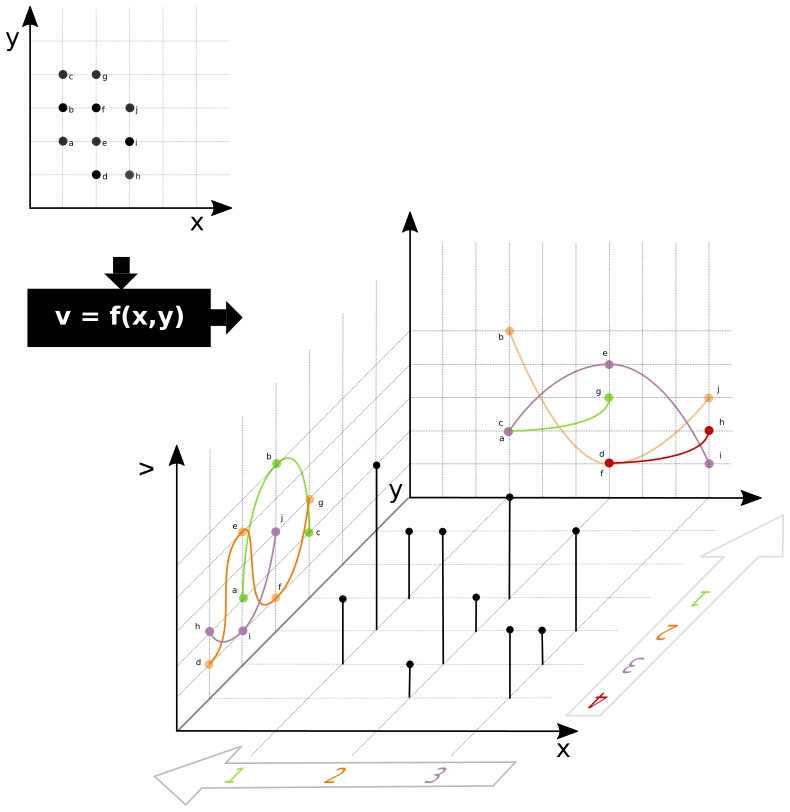
\includegraphics[width=.9\linewidth]{espaceP_espaceO_multimodal.pdf}
	\end{sidecaption}
\end{figure}

L'objectif est rendu complexe car la relation entretenue entre ces deux espaces, celui des solutions candidates disponibles, et celui des évaluations est bien souvent dissymétrique. Pour mieux comprendre cette relation, la figure \ref{fig:spacePspaceOmultimodal} illustre cette correspondance des solutions candidates $\{a \dotsc n\}$ décrites par leurs coordonnées $(x,y)$ lorsqu'elles sont projetées dans l'espace des objectifs $\mathbb{Y}$ en suivant la transformation attendue par la fonction boite noire de dynamique non linéaire $f(x,y)$. Les valeurs $v = f(x,y)$ des différentes solutions candidates sont également projetées sur le plan 2D $(x,v)$ et $(y,v)$ pour mieux visualiser la forme prise par cette surface en 2D.

\begin{figure}[!htbp]
	\begin{sidecaption}[fortoc]{Les couleurs indiquent la  des valeurs $v = f(x,y)$ mesurée dans la figure \ref{fig:spacePspaceOmultimodal}, sachant qu'on cherche à minimiser la valeur de v :
\parbox{\marginparwidth}{
\begin{enumerate}[label={},labelindent=0pt,leftmargin=*]
        \item \sqbox{tangoBlue1} indique une fitness minimale, cf. qui maximise $v$
        \item \sqbox{tangoOrange1} indique une fitness intermédiaire et,
        \item \sqbox{tangoRed1} indique une fitness maximale, cf. qui minimise $v$
\end{enumerate}}}[fig:xyspacePspaceOmultimodal]
	 \centering
	  \subbottom[]{
	 	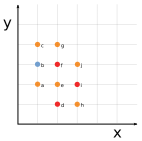
\includegraphics[width=0.4\linewidth]{xyespaceSolutionCandidate_a.pdf}
	 	\label{subfig_xyespaceSolutionCandidate_a}}
	 \subbottom[]{
	 	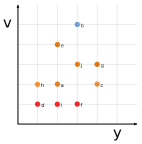
\includegraphics[width=.4\linewidth]{xyespaceSolutionCandidate_b.pdf}
	 	\label{subfig_xyespaceSolutionCandidate_b}}
	 \subbottom[]{
		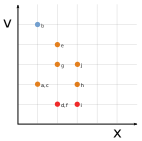
\includegraphics[width=.4\linewidth]{xyespaceSolutionCandidate_c.pdf}
		\label{subfig_xyespaceSolutionCandidate_c}}
	\end{sidecaption}
\end{figure}

Pour visualiser la valeur $v$ prise par chacune des solutions candidates, on projette celle-ci dans l'espace $(x,y)$, ce qui nous permet de mieux constater l'éclatement des valeurs de $v$ sur la figure \ref{fig:xyspacePspaceOmultimodal}.

Deux solutions proches dans l'espace des solutions candidates peuvent amener à des résultats très différents, et inversement, pour deux évaluations proches peuvent correspondre des solutions candidates très éloignées, comme le détaille la figure \ref{fig:xytrajectoire}. Il s'agit d'une propriété bien connue des fonctions non linéaires, qu'elles soient décrites de façon explicite via le formalisme mathématique, ou de façon implicite dans l'expression des dynamiques complexes de modèles de simulation.

Il est clair que l'information récoltée par un tel déplacement basé sur une distance euclidienne dans le plan $(x,y)$ n'est pas vraiment pourvoyeur d'intuitions sur l'emplacement possible des meilleures solutions (voir figure \ref{fig:xytrajectoire}). Il semble par exemple plus intéressant pour l'optimiseur d'accéder aux solutions par le prisme d'ensembles construits sur la base d'une valeur $v$ commune (voir figure \ref{fig:xyspacePspaceOmultimodal}). Une information qui peut être exploitée de multiples façons, toujours en permettant à l'optimiseur de déterminer un nouvel ensemble de solutions candidates à évaluer.

\begin{figure}[!htbp]
	\begin{sidecaption}[fortoc]{Représentation de deux déplacements dans l'espace des solutions candidates et son équivalent dans l'espace des objectifs
	\parbox{\marginparwidth}{
	\begin{enumerate}[label=(\alph*),labelindent=\parindent,leftmargin=*]
	        \item Partant de $b$, on se déplace d'une unité vers $c$ ou $a$, ce qui dans l'espace des objectifs équivaut également à un déplacement vers $h$; $v=2$ pour $v_h, v_a, v_c$
	        \item Partant de $b$, on se déplace toujours d'une unité vers $f$, ce qui dans l'espace des objectifs équivaut également à un déplacement vers $d$ et $i$; $v=1$ pour $v_d,v_i,v_f$
	\end{enumerate}}}[fig:xytrajectoire]
	 \centering
	  \subbottom[]{
	 	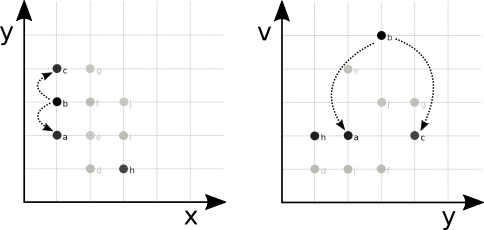
\includegraphics[width=0.6\linewidth]{xytrajectoire_a.pdf}
	 	\label{subfig_xytrajectoire_a}}\qquad
	 \subbottom[]{
	 	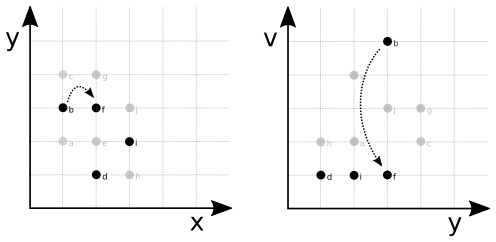
\includegraphics[width=.6\linewidth]{xytrajectoire_b.pdf}
	 	\label{subfig_xytrajectoire_b}}
	\end{sidecaption}
\end{figure}

Si l'obtention d'une cartographie complète d'un tel espace de solutions peut être l'objectif de ce type de raisonnement, la recherche d'un optimum en est un autre. Dans un cas on aura tendance à maximiser la diversité dans le choix de solutions candidates à évaluer, afin d'essayer de couvrir au mieux le territoire à explorer. Cette idée on la retrouve dans l'établissement d'une \textit{fitness landscape}, ou dans sa version multi-objectif, d'un \textit{problem landscape} \autocite[93-94]{Weise2011}, un paysage cumulé de l'espace des objectifs indiquant toutes les valeurs prises par ceux-ci au cours de l'exploration \Anote{paysage_cumule}. Un espace mis à profit par l'optimiseur pour améliorer la proposition de solution candidate, par exemple en se basant sur la construction de cluster de valeurs intéressantes comme indiqué précédemment, ou encore en cherchant à favoriser les zones de cet espace encore peu explorées, etc. Alors que dans le cas d'une optimisation pour la calibration ou la prédiction, trouver le plus rapidement possible un minimum local ou global peut constituer un objectif suffisant.

En réalité, ces deux objectifs sont souvent liés, et c'est souvent l'expertise humaine intervenant de façon externe à l'optimiseur qui va déterminer l'importance de l'un ou de l'autre dans la stratégie à suivre. Dans le cas par exemple d'une optimisation de paramètres nécessaire à la marche efficiente d'une centrale nucléaire, la découverte d'un minimum local robuste peut s'avérer beaucoup plus intéressante qu'un minimum global instable. La topologie proche de l'espace des solutions déjà exploré peut constituer un facteur de connaissance d'intervention plus ou moins importante dans l'expertise d'une bonne ou d'une mauvaise solution.

Cette mécanique on la retrouve également à un autre niveau, dans le fonctionnement interne des métaheuristiques. En effet, celles-ci s'appuient le plus souvent sur la métaphore biologique évolutive pour mettre en tension une recherche de solutions guidée toute à la fois par l'\textit{exploration} (trouver des solutions originales), et l'\textit{exploitation} (améliorer les solutions existantes).

\begin{figure}[!htbp]
\begin{sidecaption}[fortoc]{Recherche d'un minimum global.}[fig:hmap2ab]
 \centering
 \subbottom[Une fonction $f(x)$ présentant un unique minimum global]{
 	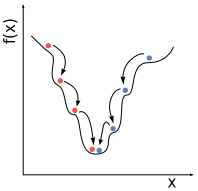
\includegraphics[width=.4\linewidth]{heightmap2a.pdf}
 	\label{subfig_hmap2ab_a}}\qquad
 \subbottom[Une fonction $f(x)$ présentant un minimum local et global]{
	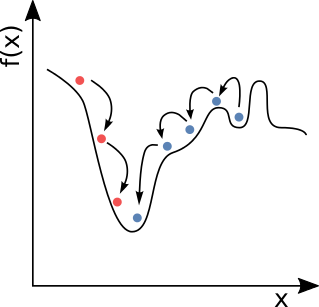
\includegraphics[width=.4\linewidth]{heightmap2b.pdf}
	\label{subfig_hmap2ab_b}}
\end{sidecaption}
\end{figure}

Les opérateurs intervenant comme stratégies dans la médiation de ces deux concepts sont conçus pour éviter à l'optimiseur un certain nombre d'écueils. Trop longue pour être abordée ici de façon exhaustive, cette liste évoquant les problèmes et solutions qui résultent du rapport entre les formes de problèmes abordés et les faiblesses génériques ou dépendantes des métaheuristiques utilisées, \textcite{Weise2011} en donne une description experte sur une centaine de pages. On peut également se référer à une autre synthèse, abordant ces problèmes avec un angle un peu plus spécifique aux algorithmes évolutionnaires, réalisée en 2001 par \textcite[316-445]{Deb2001}.

En se limitant aux pièges dépendant de la topologie de l'espace des solutions (voir point \ref{enum_meta_e}), \textcite[140]{Weise2011} a proposé un tableau synthétique dont on extrait ici quelques exemples légèrement modifiés pour éclairer notre argumentaire. Les exemples des figures \ref{fig:hmap2ab} et \ref{fig:hmap2cd} mettent en oeuvre un optimiseur générant de façon incrémentale de nouvelles solutions, chacune représentée par un point. Il faut donc lire ces exemples en tenant compte du fait qu'ils présentent une représentation cumulative des différents points parcourus dans le temps par l'optimiseur.

La figure \ref{fig:hmap2ab} démontre un fonctionnement normal de l'optimiseur, capable quelque soit son placement initial (rouge ou bleu), de trouver le minimum global d'une fonction relativement simple \ref{subfig_hmap2ab_a}. Un comportement équivalent est observable dans la figure \ref{subfig_hmap2ab_b}, le compromis \enquote{exploitation - exploration} étant suffisant pour que l'optimiseur bleu surmonte l'obstacle posé par la présence d'un minimum local dans cette fonction.

\begin{figure}[!htbp]
  \begin{sidecaption}[fortoc]{Deux types de fonctions sont rendues difficiles à optimiser du fait d'une topologie marquée.}[fig:hmap2cd]
  \centering
  \subbottom[Une fonction $f(x)$ multimodale acceptant plusieurs minimum locaux, et un seul minimum global]{
  	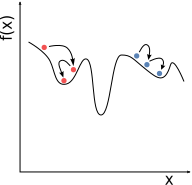
\includegraphics[width=.4\linewidth]{heightmap2e.pdf}
  	\label{subfig_hmap2cd_c}}\qquad
  \subbottom[Une fonction $f(x)$ contenant très peu d'information de gradient pour guider l'optimiseur]{
	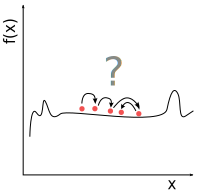
\includegraphics[width=.4\linewidth]{heightmap2c.pdf}
  	\label{subfig_hmap2cd_d}}
 \end{sidecaption}
\end{figure}

A l'inverse, on perçoit bien sur ce schéma \ref{subfig_hmap2cd_c} quel effet peut avoir un déséquilibre entre les deux stratégies, une exploitation trop appuyée au détriment de l'exploration amenant souvent à une convergence \Anote{def_convergence} prématurée, c'est-à-dire à un piège dans un optimum local.

La figure \ref{subfig_hmap2cd_d} montre également que face à une topologie de fonction présentant un plateau relativement uniforme, l'optimiseur sera en peine pour trouver un minimum, même local. Un paramétrage différent de l'exploration pourra peut être résoudre ce problème, sans pour autant que l'on en soit sur.

Ce qui nous permet d'évoquer une faiblesse connue des métaheuristiques, héritée des remarques déjà faites sur les algorithmes d'optimisations stochastique \Anote{stochastic_note} dans laquelle on les place habituellement. La découverte garantie d'une solution globale optimale est en général difficile avec ce type d'algorithmes (voir point \ref{enum_meta_d}) \Anote{equipe_mixite}, au moins pour deux raisons :

\begin{enumerate}
\item la variabilité qui opère lors de la selection des solutions candidates à un instant $t$ ne permet pas de garantir qu'il n'existe pas quelque part une solution candidate sélectionnée à $t+1$ dont l'évaluation révélera un meilleur optimum. La définition d'un critère d'arrêt est donc rendue délicate.
\item La variabilité dans l'établissement d'une trajectoire de recherche implique qu'un algorithme de même qualité puisse passer une première fois à coté d'un optimum, et une deuxième fois trouver celui-ci.
\end{enumerate}

\begin{figure}[!htbp]
\begin{sidecaption}[fortoc]{Représentation d'une navigation indirecte de l'optimiseur dans un espace de solution $z = f(x,y)$.}[fig:hmap1]
  \centering
  \subbottom[]{
  	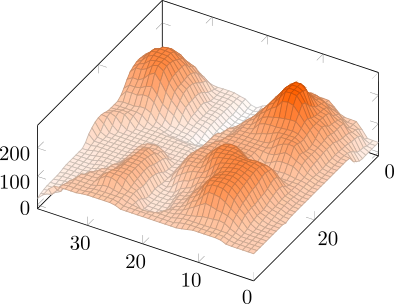
\includegraphics[width=.4\linewidth]{heightmap1a.png}
  	\label{subfig_hmap_a}}\qquad
  \subbottom[]{
	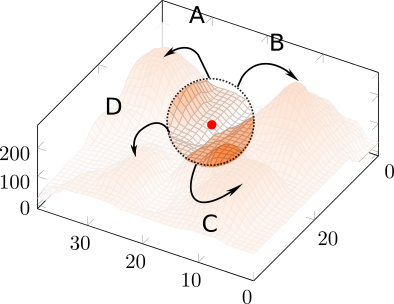
\includegraphics[width=.4\linewidth]{heightmap1b.png}
  	\label{subfig_hmap_b}}
\end{sidecaption}
\end{figure}

Pour mieux comprendre les problèmes posés par des espaces de solutions multi-modaux, déjà figurés en deux dimensions dans \ref{subfig_hmap2cd_c}, on représente cette fois ci dans la figure \ref{fig:hmap1} l'optimiseur dans un espace en trois dimensions similaire à celui vu dans la figure \ref{fig:spacePspaceOmultimodal}, à la recherche d'un optimum global. La fonction ainsi représentée comporte deux entrées $(x,y)$, et une sortie $z = f(x,y)$ représentant la valeur numérique résultat de l'optimisation.

Attention à la lecture de ces schémas, il ne faut pas oublier que l'optimiseur \textbf{ne se déplace pas directement} sur le terrain visible dans la figure \ref{subfig_hmap_a}, et pour laquelle celui-ci n'a justement aucune visibilité. C'est un peu comme visualiser un labyrinthe de l'extérieur sur une feuille, puis de l'intérieur quand on s'y projette, la difficulté pour résoudre celui-ci n'est plus la même. La visibilité dont dispose l'optimiseur est celle des résultats de solutions candidates déjà évaluées (voir point \ref{enum_meta_i}). Il s'agit donc de proposer de nouvelles solutions candidates soit en les composant à partir d'une manipulation des solutions candidates déjà évaluées, soit en introduisant de toutes nouvelles solutions candidates prises de façon aléatoire. Au cours de l'itération mesurant la progression de l'algorithme, c'est bien l'évaluation de cette nouvelle population de solutions candidates qui détermine si il y'a effectivement eu un déplacement qualitatif dans l'espace des solutions evaluées. Le déplacement du point rouge dans cet espace n'est donc effectif que si on trouve à un instant $t + 1$ une solution plus intéressante qu'à l'instant $t$.

A partir des résultats de la première solution candidate évaluée figurée ici en rouge dans \ref{fig:hmap1}, les opérateurs de recherches soumis à l'aléa d'une recomposition ou d'un tirage aléatoire peuvent tout à fait proposer un candidat à $(x,y)_{t+1}$ qui débouche sur un résultat $z = f(x,y)$ plaçant l'optimiseur dans le sillon d'un gradient de pente parmi plusieurs. Ce qui mènera probablement l'optimiseur à découvrir des optimums de qualités très différentes : $A$ (local), $B$ (global), $C$ (local), $D$ (local).

Autrement dit, en plus de la stochasticité inhérente de ces algorithmes, non seulement un algorithme de type $A$ n'aura pas les mêmes résultats qu'un algorithme de type $B$, mais celui-ci sera également différent d'un algorithme $A'$ du fait d'un paramétrage différent.

Comme déjà évoqué dans les différentes définitions, on retrouve ici la qualité de flexibilité des métaheuristiques, permettant de transformer ce qui pourrait de prime abord paraitre pour un défaut, en qualité. L'utilisation de celle-ci permettant d'étendre toujours un peu plus leurs champs d'utilisation, en facilitant la réponse aux questions suivantes \Anote{q_ppr} :
\begin{enumerate}
\item  \foreignquote{english}{What parameter settings do I use to get good results when applying heuristic method X to problem Y?}
\item  \foreignquote{english}{How do I adjust the parameters of heuristic X so I get better results on problem Y?}
\item \foreignquote{english}{Which is \enquote{better}, heuristic X or heuristic Y?}
\end{enumerate}

On pourrait ainsi ne retenir que cette citation de source inconnue, lorsqu'elle définit une métaheuristique comme \foreignquote{english}{ a pretty good rule for finding pretty good rules.}

Cette flexibilité vient compléter et compenser efficacement cet horizon de connaissance assez limité, nécessaire à une généricité d'emploi. Les métaheuristiques fournissent ainsi le support générique initial pour en faire un outil d'usage indépendant du problème, tout en fournissant les outils pour favoriser également leur propre modification en vue d'une amélioration de résultat pour un problème donné. Elle cumule donc en quelques sortes les deux propriétés de dépendance et d'indépendance face à un problème donné.

De plus, la recherche dans cette discipline ne se contente pas d'organiser une forme de compétition qui mènerait à elle seule, par l'apprentissage répété de fonctions aussi standardisées que celles utilisées dans les figures précédentes, à une surestimation de certains algorithmes \Anote{test_fonction_surutilisation}, et se nourrit également d'une recherche plus appliquée à des problématiques réelles. Ce qui permet par effet retour, d'espérer voir appliquer à des formes de problèmes génériques, des opérateurs dédiés à l'origine à des problématiques spécifiques. La construction et l'évaluation d'heuristique plus performante servant toujours indirectement une cause plus générale.

Enfin, une des propriétés qui n'a pas encore été introduite dans ce résumé est la capacité de notation et de description abstraite des métaheuristiques (voir point \ref{enum_meta_f} ). Des concepts de plus haut niveau sont introduits pour désigner l'expression et la manipulation d'heuristiques et de classes d'heuristiques dans un système composant la métaheuristique. Mais avant de pouvoir introduire ces subtilités de typologie propre à chaque classe de métaheuristique, il faut également rappeler l'existence d'une base commune de formalisation mathématique permettant la description des problèmes. Autrement dit, cela revient à introduire ou à poser sur une partie des mots déjà utilisés dans cette section, un certain nombre de notations mathématiques d'utilisation relativement standard dans cette communauté informatique utilisant les métaheuristiques.

Il nous restera également à aborder dans la section suivante, la question des \textbf{moyens} mis à disposition de l'optimiseur pour opérer la selection de nouveaux candidats à évaluer. Jusqu'ici seule une représentation de ces solutions candidates dans l'espace des solutions candidates possibles a été abordée, ainsi que l'espace contenant les résultats des solutions candidates évaluées. Mais ces deux espaces ne constituent pas les véritables espaces sur lesquels l'optimiseur est amené à travailler, et cela bien qu'il puisse les intégrer à son expertise pour la selection de nouveaux candidats à l'évaluation \Anote{remarque_section_metaheuristique}.

\hl{les 4 paragraphe ci dessous sont à faire descendre avec notation mathématique, pour compléter la section suivante, et sans briser le suspens ?}

L'introduction d'un nouvel \enquote{espace de recherche} est nécessaire, et  correspond à la somme des entrées, des paramètres, sur lequel l'optimiseur va pouvoir jouer directement, afin de modifier cette fois-ci indirectement l'expression de la solution candidate ensuite évaluée.

Autrement dit, il faut retenir qu'une solution candidate fait partie d'un espace de solutions candidates possibles, et que l'exploration de ce dernier est dépendant des bornes fixées par l'expert pour délimiter l'espace de recherche de chacun des entrant, notamment pour limiter le champ de recherche de l'optimiseur à celui des valeurs empiriquement et théoriquement possibles. Ce qui introduit aussi la possibilité d'une nouveau \textit{mapping} entre les valeurs de ces deux espaces, de recherche, et du phénomène à évaluer, qui ne sont pas nécessairement de même nature.

On peut s'appuyer sur l'exemple de bras robotisé donné par \autocite{Weise2011} pour illustrer ce cas. On a d'un côté les paramètres de positionnement des éléments de bras d'un robot, contraint par la structure théorique de celui-ci, et de l'autre l'expression spatiale finale du bras représentatif de cette combinaison de paramètres dans l'espace des solutions possibles, potentiellement infini, et dont on n'a pas la maitrise directe. L'optimiseur s'appuie ensuite sur l'évaluation de cette configuration spatiale à l'aide des critères qu'on lui a donné pour induire des opérations non pas dans l'espace d'expression spatialisé du bras, mais dans l'espace de recherche des vecteurs de paramètres permettant l'amélioration de ce résultat.

\subsubsection{Une formulation mathématique standardisée pour encadrer les problèmes d'optimisations et les métaheuristiques}
\label{sssec:math_opti}

%search space p 82
%structure p 101
% pareto ranking p 275

Pour comprendre comment se déroule de façon générale la résolution d'un problème d'optimisation, il faut poser un certain nombre de notions qui nous seront utiles par la suite. Cet exercice de description plus mathématique et générique s'appuie là encore principalement sur les écrits de \textcite{Weise2011}

La première étape selon Weise dans la construction d'un problème d'optimisation est de définir le type de structure qui peut être associée à l'expression des solutions possibles et spécifiques à notre problème.

Autrement dit, il s'agit de déterminer quel est l'espace dans lequel évolue la donnée figurant la solution attendue pour cette optimisation. L'expression de cette solution peut appartenir à l'espace des réels $\mathbb{R}$, comme par exemple une valeur numérique se rapportant à l'optimisation d'une fonction mathématique. Mais celle-ci peut également s'exprimer dans un repère beaucoup plus complexe, en faisant référence par exemple à un repère géométrique définissant le cadre  d'une forme à optimiser comme une pièce de moteur, une pièce d'avion, etc. \autocite[43]{Weise2011}

Cet espace du problème (\textit{problem space}) $\mathbb{X}$ est défini comme \foreignquote{english}{ [...] the set containing all elements $x$ which could be its solution.}

Une solution candidate $x$ est quant à elle définie comme \foreignquote{english}{ [...] an element of the problem space $ \mathbb{X}$ of a certain optimization problem.}

L'objectif de l'optimisation est donc de trouver par le biais d'un algorithme adapté l'ensemble des solutions candidates $x^*$ appartenant à l'espace du problème répondant le mieux aux critères définis par l'utilisateur. Ce qui suppose de pouvoir qualifier une solution candidate $x_1$ tiré de $\mathbb{X}$ par rapport à une autre solution candidate $x_2$ elle aussi tiré de $\mathbb{X}$.

\textit{Une deuxième étape logique serait donc d'établir comment se fait la mesure établissant la qualité d'une solution ?}

Comme défini précédemment, ce qui va guider l'algorithme optimiseur dans sa prise de décision, c'est l'évaluation d'une fonction heuristique, ou d'une fonction objectif (\textit{objective function}) \Anote{difference_objective_heuristique}

\foreignquote{english}{An objective function $f: \mathbb{X} \mapsto \mathbb{R}$ is a mathematical function which is subject to optimization.}

Cette fonction objectif lorsqu'elle prend pour paramètre un élément candidat $x$ pris dans l'espace du problème $ \mathbb{X}$ renvoie une valeur définissant sa qualité par rapport au problème posé. \autocite[44]{Weise2011}

\sloppy La plupart des problèmes nécessitent toutefois d'optimiser plusieurs critères simultanément. La relation entre ces critères peut d'ailleurs être elle aussi multiple : dépendante (conflictuelle, en harmonie), indépendante. Nous allons donc nous intéresser directement à la définition de ce type de problème, résumable ainsi :  $min(f_1(x), \dotsc, f_k(x)$ avec $k > 2$

La littérature fait également plus souvent référence à ce type de problème en faisant appel à une notation sous forme de fonction vecteurs. Un ensemble $\vec{f} : \mathbb{X} \mapsto \mathbb{R}^n$ fait de $n$ fonction objectif $f_i : \mathbb{X} \mapsto \mathbb{R}$ avec $\forall i \in 1 \dotsc n$. Appliqué à une solution candidate $x \in \mathbb{X}$ cette fonction renvoie un vecteur de réel de dimension $n$ qui peuvent être projeté dans un espace $\mathbb{R}^n$, aussi appelé espace des objectifs (\textit{objective space}) $\mathbb{Y}$.

En résumé, à chaque association d'un vecteur de fonction objectif $\vec{f}$ et d'une solution candidate $x$ correspond après évaluation un vecteur de réel de dimension $n$ permettant le positionnement de la solution candidate dans l'espace $\mathbb{R}^n$ des objectifs aussi nommé $\mathbb{Y}$.

C'est à partir du positionnement des solutions candidates dans cet espace $\mathbb{Y}$ que l'optimiseur va décider de la prochaine solution candidate à évaluer.

\begin{framewithtitle}[bla]{bla}

Pour le modèle \textbf{Ants}, on a vu qu'il existait trois paramètres pouvant être amené à varier en entrée du modèle.


Les paramètres d'évaporation $Evaporation-rate$ et $Diffusion-rate$ varie chacun dans le domaine $\mathbb{R}$, entre les valeurs $0.0$ et $99.0$ auquel on associe maintenant trois fonctions objectifs.

Le paramètre de population est réglé par défaut à $125$ fourmis dans la colonie, mais il est également possible de le faire varier sur $\mathbb{N}$ entre $0$ et $250$.

\begin{itemize}[noitemsep,nolistsep]
\item L'espace $\mathbb{X}$ est un cube $\{\mathbb{N},\mathbb{R},\mathbb{R}\}$ de bornes $\{[0,250], [0,99.0], [0,99.0]\}$
\item L'espace $\mathbb{Y}$ associe pour un point $x \in \mathbb{X}$ un point de valeur ${f_1,f_2,f_3}$ dans le domaine non borné $\{\mathbb{R},\mathbb{R},\mathbb{R}\}$
\end{itemize}

Les fonctions objectifs $\{f_1,f_2,f_3\}$  se base chacune sur le temps écoulé entre le début de la simulation $t_0$ et le temps indiqué pour la disparition complète d'un tas de nourriture.

\begin{enumerate}[noitemsep,nolistsep]
\item $f_1$ stocke le pas de temps de simulation (\textit{ticks}) à laquel le tas 1 disparait.
\item $f_2$ stocke le pas de temps de simulation (\textit{ticks}) à laquel le tas 2 disparait.
\item $f_3$ stocke le pas de temps de simulation (\textit{ticks}) à laquel le tas 3 disparait.
\end{enumerate}

Pour pouvoir rapporter ces valeurs à l'optimiseur, encore faut-il que cette simulation se finisse d'une façon ou d'une autre. Il faut donc fixer \textbf{une condition d'arrêt} pour remplacer le clic sur le bouton stop effectué par l'utilisateur dans Netlogo. La condition d'arrêt la plus simple ici est de stopper la simulation lorsque il n'y a plus aucune nourriture disponible.

Attention toutefois, il faut savoir que l'optimiseur, dans ses multiples tentatives pour trouver le meilleur jeu de valeur de paramètres qui mimise les trois fonctions objectifs risque de produire des combinaisons qui peuvent mettre le modèle ou les hypothèses du modèle en difficulté. \textit{Effectivement que se passe-t-il dans notre modèle de simulation si les valeurs de paramètres sont les suivants ? }

\begin{table}[H]
\centering
\caption{Testons ces conditions avec une même graine aléatoire (42)}
\label{tab:experience}
\begin{tabular}{lllll}
\hline
  & $Population$ & $Evaporation-Rate$ & $Diffusion-Rate$ & $t_{stop}$ \\ \hline
1 & 125        & 25.0             & 25.0  & 1554 \textit{ticks} \\
2 & 0          & 25.0             & 25.0  & $\infty$ \\
3 & 25         & 25.0             & 25.0  & 8825 \textit{ticks} \\
4 & 125        & 0.0              & 0.0   & 1374 \textit{ticks} \\
5 & 125        & 99.0             & 0.0   & 1261 \textit{ticks} \\
6 & 125        & 0.0              & 99.0  & 1201 \textit{ticks} \\
7 & 125        & 99.0             & 99.0  & 1254 \textit{ticks} \\ \hline
\end{tabular}
\end{table}

Dans Le cas (2) la simulation ne s'arrête jamais, car la condition d'arrêt n'est jamais rempli. Ce comportement n'est clairement pas intéressant et risque tout simplement de bloquer l'exploration réalisé par la métaheuristique, il faut donc fixer un seuil > 0 à cette population initiale de fourmis.

Le cas (3) montre qu'avec moins de fourmis, il faut beaucoup plus de temps à la simulation pour que la condition d'arrêt soit rempli. Il peut donc y'avoir une très forte variabilité dans les durées d'execution du modèle en fonction des valeurs de paramètres selectionné pour évaluation.

Le cas (4,5,6) sont intéressant, car ils sont susceptible de produire des résultats contre-intuitifs. En effet, en terme de durée d'execution totale, on obtient pour cette graine aléatoire de meilleurs résultats qu'avec des valeur de paramètres pris au hasard (1). Un mauvais paramétrage produit un effet d'aspiration qui fait que des fourmis normasont détournés par une piste olfactive.

\begin{figure}[H]
	 \centering
	 	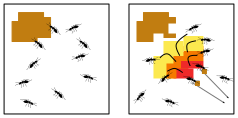
\includegraphics[width=.9\linewidth]{ant.pdf}
\end{figure}

Cela peut également s'expliquer par le débordement et la mise en défaut des mécanismes prévu initialement par le modélisateur, car les fourmis ne captent les traces chimique qu'entre $0.05$ et $2$. Or la diffusion ou l'évaporation se cumule en partant d'une valeur unitaire à $60$, qui est l'équivalent de la trace chimique déposé sur chaque patch pour une fourmi ayant trouvé de la nourriture. Donc dans tout ces ce cas là, les mécanismes du modèle sont quasi-inneficace, et se rapport au cas (3) qui met en jeu une simple marche aléatoire des fourmis.

\textit{L'optimiseur sera-t-il capable de trouver de meilleures valeurs dans cette zone d'activation ?} Si non, il faudra revoir les paramètres ou le fonctionnement de notre mécanisme guidant le comportement de dépot et de détection de trace de chaque fourmi.

Plusieurs pistes peuvent être indiqués au modélisateur pour éviter ou limiter l'apparition de comportement pouvant bloquer l'exploration :

\begin{itemize}[noitemsep,nolistsep]
	\item Fixer les valeurs de paramètres pouvant poser problème, quitte à les faire varier par la suite
	\item Identifiez en amont les combinaisons de jeu de valeurs de paramètres susceptible de poser problème, pour ensuite les interdire à l'optimiseur
	\item Introduire un paramètre ou un mécanisme artefact (c'est-à-dire qui est extérieur aux hypothèses originales) dans le modèle, par exemple en limitant le nombre de tortue évoluant pour une espèce donnée
	\item Introduire des critères d'arrêt plus restrictif
	\item Pénaliser les comportements posant problèmes dans les fonction objectifs
\end{itemize}

Un autre type d'erreur peut encore intervenir lors de telle exploration, la combinatoire de paramètre pouvant faire apparaitre des erreurs dans le déroulement de votre programme (division par zéro, comportement innatendus, dépassement mémoire, etc.) En ce sens, ce type d'exploration participe de la validation interne du modèle.

\end{framewithtitle}

\textit{Dès lors, comment ce choix se fait-il dans une perspective multi-objectifs a priori contradictoires ?}

\begin{figure}[!hbtp]
	\begin{sidecaption}[fortoc]{ Pour la valeur $x = 0$, $f1(x) = 0 $ et $f2(x) = 4 $, pour $x = 2$,  $f1(x) = 4 $ et $f2(x) = 0 $ , donc la configuration inverse. La solution pour minimiser les deux fonctions $f1$ et $f2$ tient donc forcément dans un compromis dans la valeur prise par $x$.}[fig:S_Schaffer]
	\centering
	\begin{tikzpicture}[line cap=round,line join=round,>=triangle 45,x=1.0cm,y=1.0cm]
	\draw [color=cqcqcq,dash pattern=on 1pt off 1pt, xstep=1.0cm,ystep=1.0cm] (-5,-1) grid (5,5);
	\draw[->,color=black] (-5,0) -- (5,0);
	\foreach \x in {-5,-4,-3,-2,-1,1,2,3,4}
	\draw[shift={(\x,0)},color=black] (0pt,2pt) -- (0pt,-2pt) node[below] {\footnotesize $\x$};
	\draw[->,color=black] (0,-1) -- (0,5);
	\foreach \y in {-1,1,2,3,4}
	\draw[shift={(0,\y)},color=black] (2pt,0pt) -- (-2pt,0pt) node[left] {\footnotesize $\y$};
	\draw[color=black] (0pt,-10pt) node[right] {\footnotesize $0$};
	\clip(-5,-1) rectangle (5,5);
	\draw[color=ttttff] plot[raw gnuplot, id=func2] function{set samples 100; set xrange [-4.9:4.9]; plot x**2};
	\draw[color=fftttt] plot[raw gnuplot, id=func3] function{set samples 100; set xrange [-4.9:4.9]; plot (x-2)**2};
	\begin{scriptsize}
	\draw[color=ttttff] (-2.26,6.14) node {$f$};
	\draw[color=fftttt] (-0.24,6.14) node {$g$};
	\end{scriptsize}
	\end{tikzpicture}
 \end{sidecaption}
\end{figure}

\sloppy Si on prend pour exemple la fonction multi-objectifs de Schaeffer décrite dans l'équation \ref{eq:schaffer}, $f1(x)$ and $f2(x)$ deux fonctions objectifs à minimiser $\vec{f} = (f1(x),f2(x))^T$  avec $\vec{f}: \mathbb{X} \mapsto \mathbb{R}^2$

\begin{equation} \label{eq:schaffer}
Minimize =
	\begin{cases}
	 f1(x) = x^2 \\
	 f2(x) = (x-2)^2
	\end{cases}
\end{equation}

Si on superpose les deux fonctions comme dans la figure \ref{fig:S_Schaffer}, on voit bien qu'elles sont contradictoires, il s'agit donc de trouver un compromis.

Cette opération que nous pratiquons tous les jours sans forcément le savoir peut être plus facilement expliquée en faisant appel à cet exemple concret. Dans le cas d'un acheteur à la recherche d'une voiture à la fois économe de par sa faible consommation et si possible disponible à un moindre coût, celui-ci devra bien se plier à l'exercice de positionnement des voitures résumé dans le graphique \ref{fig:voiture}.

Dans le graphique \ref{subfig_voiture:b} on constate rapidement que le modèle de voiture que l'acheteur va acheter à de fortes chances de se trouver dans la liste de voitures $\{ A,B,C,D,E \}$ colorées en rouge, aussi appelée front de Pareto, ou optimum de Pareto. Ce terme apparait en économie en 1950, en référence directe des travaux de l'économiste italien Vilfredo Pareto. Le lecteur plus curieux de ces questions pourra trouver de multiples points d'entrées sur ces questions dans les publications suivantes \autocites{Ehrgott2012,Koksalan2011,Koksalan2013}.

\begin{figure}[!htbp]
	\begin{sidecaption}[fortoc]{Exemple simplifié d'une catégorisation de voitures selon deux axes comprenant d'une part le coût d'achat et d'autre part la consommation de chaque voiture.}[fig:voiture]
	\centering
	  \subtop[]{
  	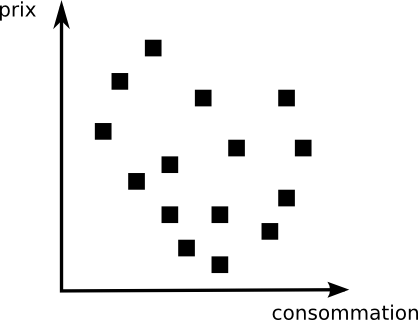
\includegraphics[width=.3\linewidth]{opti1.png}
  	\label{subfig_voiture:a}}\qquad
    \subtop[]{
	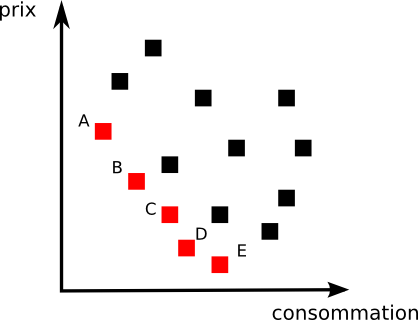
\includegraphics[width=.3\linewidth]{opti2.png}
  	\label{subfig_voiture:b}}
    \subtop[]{
  	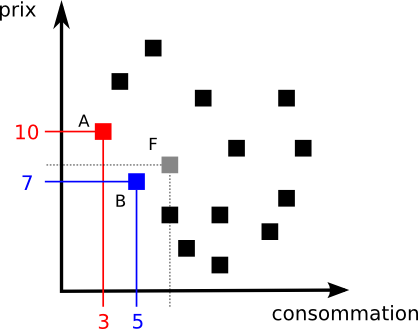
\includegraphics[width=.3\linewidth]{opti3.png}
  	\label{subfig_voiture:c}}
 \end{sidecaption}
\end{figure}

\sloppy En regardant en détail les capacités des voitures figurant dans ce front \ref{subfig_voiture:c}, on voit bien que chacune d'entre elle domine une partie des autres voitures sur au moins un des deux objectifs. Si on prend le cas de la voiture F, celle-ci n'est pas prise en compte dans les solutions optimums, car le point est dominé sur ses deux objectifs par d'autres voitures : $ prix(B) < prix(F) < prix(A) $ et $consommation(A) < consommation (B) < consommation(F)$.

Le front de Pareto renvoie un ensemble de solutions compromis optimal, l'expertise finale sur la ou les solutions à adopter est donc le résultat d'un choix expert externe introduit comme support à l'algorithme optimiseur. Dans notre exemple, l'acheteur devra pour finaliser son achat mettre en avant au moins un des deux critères afin de départager les voitures.

Si certains algorithmes ont introduit cette expertise par le biais d'une sélection interactive guidant l'optimiseur à chaque étape de sa recherche, ce n'est pas cette usage qui nous intéresse ici. L'expertise n'intervient qu'une fois les solutions convergées, dans l'observation des résultats finaux.

Dans notre cas, on considère que l'optimiseur doit sélectionner avec les moyens qu'on lui a fournis les solutions candidates sur lesquels il doit miser pour converger. Il doit donc être capable de séparer les solutions en appliquant un ou plusieurs critères de séparation. Il existe plusieurs types de stratégies (\textit{Agreggation based, Criterion based, Dominance based, Indicator based}), et chacune d'elles peut être croisée ou dérivée en de multiples variantes \autocites[28]{Zitzler1999a, Deb2001}[7]{Liefooghe2009}. Nous limiterons ici notre analyse à un seul de ces cas, en nous focalisant d'ores et déjà sur les méthodes les plus utilisées en EC, basées sur la dominance celles-ci sont directement inspirées des travaux de Pareto.

% TODO : Finir ce paragraphe historique rapide, qui permettra de faire la différence ensuite avec les algorithmes inspirés par Pareto.
% TODO : Ajouter ref de Goldberg sur les sciences humaines + GA dans le chapitre 1

\begin{figure}[!htbp]
	\begin{sidecaption}[fortoc]{Graphique en deux dimensions des fonctions objectifs $f_1$ et $f_2$ du tableau \ref{tab:pranking}}[fig:pranking_a]
		\centering
		
\includegraphics[width=.4\linewidth]{pareto_ranking_a.pdf}
	 \end{sidecaption}
\end{figure}

\begin{table}[!htbp]
\begin{sidecaption}[fortoc]{Tableau de résultats des fonction objectifs $f_1$ et $f_2$ pour un vecteur de solutions candidates $\{a \dotsc p\}$ dans l'espace des objectifs $\mathbb{Y}$, et résultat du \textit{Pareto Ranking}, intervenant ensuite dans le calcul de \textit{fitness} de différentes façons selon les algorithmes utilisés :
 \parbox{\marginparwidth}{
 \begin{enumerate}[label=(\alph*),labelindent=0pt,leftmargin=*]
	      \item $v_1$ est une \textit{fitness} calculée sur la base du nombre de dominé $+ 1$, cf. une partie de calcul de fitness de l'algorithme MOGA de \textcite{Fonseca1993}.
	      \item $v_2$ est une \textit{fitness} calculée sur la base du calcul de fronts de l'algorithme NDS de \textcite{Goldberg1989}.
	\end{enumerate}}}
	[tab:pranking]
	\centering
	\begin{tabular}{>{$}l<{$} >{$}l<{$} >{$}l<{$} >{$}l<{$} >{$}l<{$} >{$}l<{$}}
			\toprule
			\text{solutions candidates} & f_1 & f_2 & \text{dominé par} & v_1 & v_2 \\
			\midrule
			a      & 3.5    & 1    &  \varnothing & 1 & 1 \\
			b      & 3      & 1,5  &  \varnothing & 1 & 1 \\
			c      & 2      & 2    &  \varnothing & 1 & 1 \\
			d      & 1      & 3    &  \varnothing & 1 & 1 \\
			e      & 0.5    & 4    &  \varnothing & 1 & 1 \\
			f      & 0.5    & 4.5  &  \{e \}      & 2 & 2 \\
			g      & 1.5    & 4.5  &  \{d,e,f,h \} & 5 & 3 \\
			h      & 1.5    & 3.5  &  \{d \}      & 2 & 2 \\
			i      & 2      & 3.5  &  \{c,d,h \}  & 4 & 3 \\
			j      & 2.5    & 3    &  \{c,d \}    & 3 & 2 \\
			k      & 3.5    & 2    &  \{a,b,c \}  & 4 & 2 \\
			l      & 4.5    & 1    &  \{a \}      & 2 & 2 \\
			m      & 4.5    & 2.5  &  \{a,b,c,k,l \} & 6 & 3 \\
			n      & 4      & 4    &  \{a,b,c,d,e,h,i,j,k,o \} & 11 & 5 \\
			o      & 3      & 4    &  \{b,c,d,e,h,i,j \} & 8 & 4 \\
			p      & 5     & 4.5   &  \{a,b,c,d,e,f,g,h,i,j,k,l,m,n,o \} & 16 & 6 \\
			\bottomrule
	\end{tabular}
  \end{sidecaption}
\end{table}

Pour comprendre comment cette stratégie et définir mathématiquement la notion d'optimum de Pareto, il faut introduire la notion de \textit{dominance} sur lequel elle s'appuie. Pour cette tâche on s'appuie sur les définitions données par \textcite[65]{Weise2011} :

\foreignquote{english}{An element $x_1$ dominates (is preferred to) an element $x_2 (x_1 \dashv x_2)$ if $x_1$ is better than $x_2$ in at least one objective function and not worse with respect to all other objectives.}

Ce qui dans le cas d'une minimisation se traduit mathématiquement par les conditions suivantes :

% TODO : A CORRIGER ABSOLUMENT AVEC WEISE !!
\begin{align*}
	(x_1 \dashv x_2) \Leftrightarrow &\forall i \in 1 \dotsc n \Rightarrow  f_i (x_1) \leq f_i (x_2) \land \\
	&\exists j \in 1 \dotsc n : f_j (x_1) < f_j (x_2)
\end{align*}

Cette notion de \textit{domination} ($\succ$) \Anote{notation_dominance} permet de dégager ces trois possibilités

\begin{itemize}
\item $x_1$ domine $x_2$ , qui peut également s'écrire $x_1 \succ x_2$
\item $x_1$ est dominé par $x_2$
\item $x_1$ n'est pas comparable avec $x_2$
\end{itemize}

Celle-ci possède les propriétés suivantes, qui définissent dans l'espace des objectifs $\mathbb{Y}$ un \textit{strict partial order} :

\begin{enumerate}
\item{\textbf{non reflexive}}  $x_1$ ne peux pas se dominer lui même
\item{\textbf{non symétrique}} $ x_1 \succ x_2$ n'implique pas $x_2 \succ x_1$, alors que l'opposé est vrai, $x_1 \succ x_2$ implique $x_2$ ne domine pas $x_1$
\item{\textbf{transitive} }
\end{enumerate}

Différents degrés de dominance ont été développés, comme par exemple la notion de \textit{strong dominance} : $x_1$ domine fortement $x_2$ ($x_1 \succ \succ x_2$) si $x_1$ est strictement meilleur que $x_2$ sur tout ses objectifs.

Pour bien comprendre comment se construit l'ensemble $X^*$ de solutions non dominées $x^* \in \mathbb{X}$ ,on peut étudier en détail comment la dominance se calcule entre les points $e$ et $f$ présentés sur la figure \ref{fig:pranking_a}.

\begin{table}[!h]
	\centering
	\begin{sidecaption}[fortoc]{Application des règles de dominance aux points $e$ et $f$. \\ \\
		   \begin{tabular}{>{$}l<{$}>{$}l<{$} >{$}l<{$}}
					\toprule
					 & f1 & f2 \\
					\midrule
					e      & 0.5    &  4   \\
					f      & 0.5    & 5,5  \\
					\bottomrule
			\end{tabular}\\ \\
			(a) $e \succ f$ car e est bien le meilleur sur au moins un des deux objectifs, et n'est pas pire sur aucuns des autres objectifs ($e \succeq f$ ) \\
			(b) f ne domine pas e car f n'est pas meilleur sur aucun des deux objectifs et il est pire sur au moins un des deux objectif}[tab:pranking]

		\begin{minipage}{0.5\textwidth}
			\centering
			\subbottom[e est dominé par f ?]{
				\begin{tabular}{>{$}l<{$}>{$}l<{$} >{$}l<{$}}
					\toprule
					    & f1 & f2 \\
					\midrule
					e \leq f & \text{true} & \text{true} \\
					e < f   & \text{false}  & \text{true} \\
					\bottomrule
				\end{tabular}
		 	\label{pranking_a}}
		 \end{minipage}\hspace{1em}
		 \begin{minipage}{0.5\textwidth}
		 	\centering
			\subbottom[f est dominé par e ?]{
				\begin{tabular}{>{$}l<{$}>{$}l<{$} >{$}l<{$}}
					\toprule
					  & f1 & f2 \\
					\midrule
					f \leq  e & \text{true} & \text{false} \\
					f < e  & \text{false}  & \text{false} \\
					\bottomrule
				\end{tabular}
			\label{pranking_b}}
		\end{minipage}
  \end{sidecaption}
\end{table}

Les solutions admises parmi le front de Pareto (voir figure \ref{fig:frontoptimal}) sont donc ici toutes celles qui ne sont pas dominées faiblement ($\succeq$), ce qui revient à exclure les points $f$ et $l$ du front optimum $\{a,b,c,d,e\}$ car ils sont dominés faiblement ($e \succeq f$); alors que dans le cadre d'une dominance forte ($\succ \succ$), ceux-ci auraient fait partie du front $\{a,b,c,d,e,f,l\}$. En effet si on prend toujours le cas de $e$ et $f$, la condition testant que $e$ est strictement meilleur que $f$ sur tous les objectifs n'est pas remplie.

%Cet ensemble de cardinalité forcément inférieure ou égale est qualifié \enquote{d'ensemble fort non dominé} (\textit{Strongly non dominated set}).

Le front de Pareto pour $\succ \succ$ est plus \textbf{grand} que le front de Pareto pour $ \succ $. Or $\succ \succ$ est \textbf{plus stricte} que $\succ$. Le raisonnement est contre-intuitif, par conséquent nous allons le dérouler plus en détail par la suite en observant de plus près le cas litigieux, c'est-à-dire pour le point $f$ et $l$, car $f_1 = e_1$

On examine si $f$ doit être exclu de l'ensemble Front de Pareto $FP$ dans les deux cas, pour une dominance forte ($\succ \succ$) et une dominance faible ($\succeq$)

\textbf{1) Dans le cas d'une dominance forte : }
\begin{align*}
     si f \notin FP & \Rightarrow \exists x \in FP \\
     & \text{tel que }  x \succ \succ f
\end{align*}
On teste tous les éléments de $FP$, le seul qui pose question est le point $e$, on pose donc la question suivante, est ce que $e \succ \succ f$ ?

\textbf{Non,} car $f_1(e) = f_1(f)$ , et donc $e$ ne domine pas fortement $f$. N'étant pas en mesure d'établir un ordre entre ces valeurs, il est impossible d'exclure $f$ de $FP$, et donc $ f \in FP_{\succ \succ}$

\textbf{2) Dans le cas d'une dominance faible : }
On reprend la définition qui nous est donné, $ e \succeq f$ si
\begin{enumerate}[label=(\arabic*),labelindent=\parindent,leftmargin=*]
\item $ \forall_i \ e_i \leq f_i$
\item $ \exists_j \ e_j < f_j$
\end{enumerate}

Or (1) est bien $True$ d'après le tableau \ref{tab:pranking}, il est donc possible d'écrire $e_1 \leq f_1$ et $e_2 \leq f_2$ Le cas (2) est également $True$ car $e_2 < f_2$

\textbf{Par conséquent}, le fait que (1) et (2) soit égal à $True$ permet, à la différence de la dominance forte, de discriminer $e$ par rapport à $f$, ce qui fait  que $e_2 \succeq f_2$. Donc $f \notin FP_{\succeq}$

\begin{figure}[!htb]
	\begin{sidecaption}[fortoc]{Tracé du front optimum à partir du calcul des individus non dominés, cf. l'ensemble vide $\varnothing$ dans le tableau \ref{tab:pranking}}[fig:frontoptimal]
		\centering
		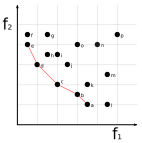
\includegraphics[width=.4\linewidth]{pareto_front.pdf}{
		}
  \end{sidecaption}
\end{figure}

Le front de Pareto n'est en général jamais entièrement couvert, cela pour diverses raisons :

\begin{itemize}
\item L'évaluation de la fonction à optimiser est souvent coûteuse, comme dans le cas de modèle de simulation dont l'exécution peut prendre jusqu'à plusieurs dizaines de minutes,
\item La zone d'exploration est volontairement bornée du fait des objectifs des expérimentateurs,
\item La stochasticité oblige l'exécution de nombreuses réplications d'une même évaluation,
\item On dispose de ressources finies, or l'espace du front est souvent continu et non borné en dehors des contraintes que l'on aura nous-mêmes fixées.
\end{itemize}

Selon \textcite[70]{Weise2011} et \autocite[19]{Zitzler1999a}, on peut s'aider dans cette tâche d'établissement d'un front de Pareto correct en étant attentif aux points suivants:

\begin{enumerate}
\item{\textbf{Proximité}} Les solutions découvertes doivent être les plus proches possibles du front de Pareto optimal.
\item{\textbf{Diversité}} Si le front optimal possible est trop large, la répartition des solutions \textit{spread} doit être maximisé sur toute la surface de celui-ci, si possible suivant une distribution uniforme.
\item{\textbf{Pertinence}} Les solutions découvertes doivent correspondre aux intérêts définis par le problème, et n'ont aucun intérêt si l'opérateur humain ne peut, ou ne sait les utiliser.
\end{enumerate}

On retrouve dans ces objectifs la tension entre exploration et exploitation, le front de Pareto devant être exploité de façon homogène, tout en garantissant à terme (et si possible le plus vite possible) la convergence vers une zone d'intérêt pour l'expérimentateur (voir figure \ref{fig:convergence_diversite}). Les métaheuristiques n'ayant pas d'apriori sur la forme de problème abordée, c'est dans l'originalité, la diversité des constructions proposées qu'une solution optimale et dédiée peut être trouvée. Il est donc très difficile de faire un listing des meilleures stratégies, et des meilleures combinaisons de stratégies permettant une sélection garantie des meilleurs candidats en fonction de ces objectifs, l'établissement de cette liste ne pouvant être que contextuelle d'un problème d'optimisation donné.

\hl{ref no free lunch theorem }? Wikipedia : Le théorème du « no free lunch » explique qu’aucune instance de métaheuristique ne peut prétendre être la meilleure sur tous les problèmes. Une métaheuristique (M) n’est performante que pour une classe de problème (P) donnée.

Heureusement, un certain nombre de combinaisons, souvent éprouvées par de multiple tests sur des fonctions aux caractéristiques et difficultés soigneusement étudiées (ZDT, etc.), se démarquent par des capacités de résolution acceptable. C'est d'ailleurs souvent sur cette première base que se construisent ensuite les améliorations nécessaires à une réponse optimale, cela en partie grâce à la flexibilité des composantes caractéristique des métaheuristiques.

\begin{figure}[!htbp]
  \begin{sidecaption}[fortoc]{Convergence et maintien de la diversité au sein du front de Pareto}[fig:convergence_diversite]
  \centering
  \subbottom[Un front de pareto sans maintien suffisant de la diversité]{
  	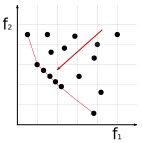
\includegraphics[width=.4\linewidth]{pareto_convergence_a.pdf}
  	\label{subfig_convergence_diversite:a}}\qquad
  \subbottom[Un front de pareto avec maintien de la diversité]{
	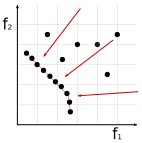
\includegraphics[width=.4\linewidth]{pareto_convergence_b.pdf}
  	\label{subfig_convergence_diversite:b}}
 \end{sidecaption}
\end{figure}

\textit{Une fois défini cet ordre partiel entre les solutions candidates évaluées, sur quelle base l'optimiseur prend sa décision pour sélectionner les individus les plus prometteurs ? et comment celui-ci garantit l'évolution des solutions candidates selectionnées au regard des trois objectifs fixés ?}

Comme le dit de façon très claire,\textcite[94]{Weise2011} \foreignquote{english}{Such comparisons, however, only state whether one candidate solution is better than another one or not, but give no information on \textbf{how much} it is better or worse and \textbf{how interesting} it is for further investigation. Often, such a scalar, relative measure is needed.}

L'optimiseur n'ayant pas les capacités pour comparer des fonctions entre elles, c'est par l'attribution d'un scalaire caractérisant chaque vecteur $z^* \in \mathbb{Y}$ résultat de l'évaluation d'une solution candidate, que celles-ci vont pouvoir être départagées. On parle de \enquote{fonction d'utilité}, ou de \enquote{fonction \textit{fitness}} pour désigner cette opération de transformation dont le résultat $z$ est utile uniquement en se plaçant dans le référentiel de l'optimiseur. Il s'agit d'un classement relatif des solutions les unes par rapport aux autres, calculés indépendamment des valeurs prises par les fonctions objectives, et intégrant un certain nombre d'autres critères, définis en réponse aux exigences des trois objectifs déjà évoqués (respect de la diversité, qualité de convergence, pertinence vis-à-vis du problème).

Ainsi, un des tout premiers paramètres à intégrer dans le calcul de cette fonction \textit{fitness} tient évidemment dans le choix d'une stratégie pour tirer un meilleur parti des informations récoltées dans l'application de cet ordre partiel sur l'espace $\mathbb{Y}$. Là ou des algorithmes vont appuyer la sélection des solutions à partir d'un calcul de rang (je ne garde que les $n$ premiers rangs), d'autres vont le faire à partir d'un décompte des non dominés (je ne garde que les individus non dominés $< n$), à partir d'une profondeur (je ne garde que les $n$ premiers fronts), ou encore en mélangeant ces trois informations (voir ces résultats dans le tableau \ref{tab:pranking}) A cela il faut également ajouter la diversité de choix à disposition dans la selection d'une dominance, par le changement de l'opérateur utilisé dans le calcul (\textit{weak dominance}, \textit{strong dominance}, etc.), ou même la relaxe de celui-ci (\textit{epsilon-dominance}). Des choix de première importance, car ils interviennent directement dans la construction de l'ensemble de solution retenue.

C'est donc dans l'espace des objectifs $\mathbb{Y}$ que se révèle la première information pertinente pour l'optimiseur, nous indiquant, peu importe la forme de l'une ou de l'autre des fonctions et le positionnement des points sur celles-ci, une première sélection de solutions parmi les solutions candidates évaluées sur laquelle l'effort de l'optimiseur doit porter en priorité.

Mais lorsque l'on reprojette les résultats du front de Pareto dans l'espace figurant la dynamique supposée de chacune des deux fonctions objectifs, on observe que la prise de décision basée sur le seul ordonnancement des solutions n'est pas suffisante pour garantir une selection optimale des meilleurs candidats à l'évolution (voir figure \ref{fig:mo_landscape}).

La forme des fonctions dans cette figure est représentée en pointillé car elle n'est qu'une description temporaire d'un paysage en partie inconnu, en attente d'être révisée par l'évaluation de nouveaux points. Le tracé d'un paysage ne se confond plus comme cela pouvait être le cas dans une optimisation mono-objectif avec la valeur prise par la fonction objectif, et doit maintenant intégrer un intermédiaire supplémentaire plus complexe qui est le calcul d'une fonction \textit{fitness}, et dont la formulation, dépendante de nombreuses stratégies, va modifier les solutions choisies dans le futur, et donc modifier la façon dont on va découvrir l'approximation de ce paysage, cela de façon indépendante aux objectifs choisis. \autocite{Weise2011}

\begin{figure}[!htbp]
	\begin{sidecaption}[fortoc]{Projection du front de Pareto optimal (point \sqbox{tangoBlack1}), et des autres solutions candidates dominées (point \sqbox{tangoGrey1}) sur l'espace de variation du paramètre $x \in \mathbb{R}$, un schéma inspiré par \textcite[67]{Weise2011}
	\parbox{\marginparwidth}{
	\begin{enumerate}[label={},labelindent=0pt,leftmargin=*]
	      \item \sqbox{tangoBlue1} $f_{1}(x)$
	      \item \sqbox{tangoRed1} $f_{2}(x)$
	\end{enumerate}}\\
	Les fonctions $f_{1}(x)$ et $f_{2}(x)$ sont représentées en pointillé car elles sont inconnues de l'optimiseur, et ne servent que de repère au lecteur pour mieux comprendre comment un paysage caractérisant l'intersection des deux fonctions peut émerger durant l'optimisation, et pourquoi cela peut être intéressant d'intégrer son analyse à l'optimiseur.}[fig:mo_landscape]
	 \centering
	 	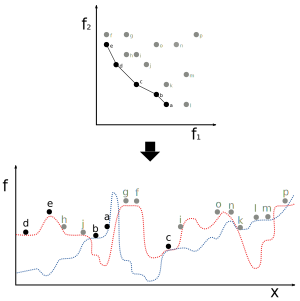
\includegraphics[width=0.8\linewidth]{multi_objective_landscape.pdf}
	\end{sidecaption}
\end{figure}

%on se rend également compte qu'un surplus d'information tiré de l'exploitation d'autres espaces pourrait être utile au choix de l'optimiseur

%\Anote{weise_multi2D}
Déjà beaucoup plus difficile à imaginer que dans l'exemple précédent de l'équation de Schaeffer, la re-projection des solutions candidates évaluées se fait sur un nouvel espace $\mathbb{G}$ (voir figure \ref{fig:relation_espaces}), qui inclu l'ensemble de tout les éléments $g \in \mathbb{G}$ qui peuvent être manipulés par les opérateurs de recherche à disposition de l'optimiseur \autocite[82]{Weise2011}. Un processus détaillé un peu plus tard dans cette section.

Dans notre cas $x \in \mathbb{R}$, on a donc un paramètre qui est manipulable et peut prendre une infinité de valeurs dans le cadre des contraintes définies pour $x$ (par exemple une valeur de 0 à 10 pour $x$) \Anote{remarque_resolution}. L'espace $\mathbb{G}$ contient la codification du problème, ce qui par exemple dans le cadre de simulation, se traduit pour chaque élément $g$ par l'attribution d'un vecteur de paramètres définissant les entrées de la simulation sur lequel l'optimiseur va pouvoir \enquote{jouer} pour optimiser les différentes fonctions objectifs.

La fonction $gpm : \mathbb{G} \mapsto \mathbb{X}$ est une translation opérée lorsque les deux espaces sont de nature différente, par exemple pour passer d'un espace Binaire à un espace de Réels $\mathbb{B} \mapsto \mathbb{R}$. Dans le cadre de simulations, les deux espaces sont souvent de nature similaire $\mathbb{G} = \mathbb{R}$. On pourra se référer à \textcite[86-88]{Weise2011} pour plus de détails.

\begin{figure}[!htbp]
	\begin{sidecaption}[fortoc]{Résumé des relations entre les différents espaces dans une optimisation}[fig:relation_espaces]
		\centering
		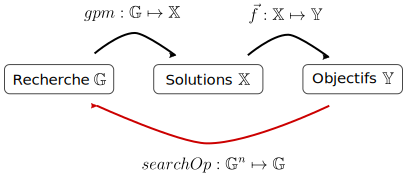
\includegraphics[width=.7\linewidth]{objectifsToSearchSpace.pdf}
  \end{sidecaption}
\end{figure}

%D'une part, l'observation de dynamiques en partie contraires sur ces deux fonctions $f_1$ et $f_2$ nous permet de constater encore une fois pourquoi un déplacement de l'optimiseur sur l'une ou l'autre des fonctions dirigé par la recherche d'un optimum n'a aucun sens.

L'opération de sélection des solutions candidates est souvent rattachée au processus de convergence. L'objectif de l'optimiseur est d'évaluer au mieux le potentiel de chacune des solutions durant cette phase de sélection pour intégrer et conserver les meilleurs éléments à son référentiel entre deux itérations. On imagine pourtant très bien bien l'effet que peut avoir une sélection trop restrictive sur le maintien de la diversité. C'est le cas par exemple si l'optimiseur ne décide de garder que le front de Pareto, on voit bien sur la figure \ref{fig:mo_landscape} à quel point la couverture de la dynamique des deux fonctions ressortirait considérablement appauvrie à la suite d'un tel choix. On en déduit que la frontière entre stratégies de convergence, et stratégie de maintien de la diversité doit être assez perméable pour garantir le choix de solutions candidates pertinentes en dehors du seul front de Pareto. Zitler \hl{ref autre que ppt à trouver} retient par exemple parmi ces classes de stratégies celle s'appuyant sur le couple associant espace des objectifs et au choix la dominance, la densité, le temps, ou encore la chance. Ce sont des heuristiques qui vont intervenir en amont sur la qualité et la diversité des solutions candidates (par exemple les stratégies de \textit{sharing}, \textit{crowding}, etc.) qui peuvent ensuite être manipulées par les opérateurs de recherches de l'optimiseur.

Viennent ensuite les stratégies de recombinaison des solutions selectionnées, créatrices de nouvelles solutions candidates à évaluer. Un processus qui peut être là aussi rattaché tout autant au maintien de la diversité qu'à une volonté de convergence accrue. Il n'y a là encore aucune règle d'applications spécifique, et tout dépend de l'objectif fixé de façon initiale ou au cours de l'expérimentation. Ainsi, certaines stratégies intégrés aux opérateurs peuvent être mis en place pour limiter une convergence trop rapide des solutions (\textit{premature convergence}) liée à une perte de diversité, alors que d'autres vont tenter d'accélérer cette convergence par la mise en oeuvre d'opérateur de recherche plus agressif, soit pour trouver le plus rapidement possible un minimum (ou maximum) local, soit car la topologie de l'espace des objectifs est de topologie difficile.

La sélection de candidats à la manipulation dans l'espace des objectifs $\mathbb{X}$ se réfère, une fois projetée dans cet espace $\mathbb{G}$, aux éléments $g$ accessibles à la manipulation par les opérateurs de recherche de la fonction $searchOp$. Chacun de ces opérateurs, dont le nombre et la nature est un paramètre de l'optimiseur, s'appuie sur la transformation d'une ou plusieurs solutions candidates dirigée par la création d'un nouvel élément $g$, dont on attend si possible un meilleur résultat à l'itération suivante. Un postulat très fort est posé par ce type de méthodes d'optimisation, l'introduction de petites variations sur les valeurs de l'espace de recherche est également censée apporter de petites variations dans l'espace des objectifs, que cela résulte en une amélioration ou en une dégradation de la qualité. Appelée \textit{strong causality} \Anote{note_strong}, cette propriété est évidemment dépendante de la forme prise par le paysage du problème (\textit{problem landscape}), et plus celui-ci est accidenté, rugueux, plus sa résolution est considérée comme complexe \Anote{note_weak}.

En relation avec cette observation, l'éclatement de cette population de solutions candidates évaluées sur le paysage nous permet de constater (voir la figure \ref{fig:mo_landscape}) à quel point la notion de distance entre les points parait différente entre ces deux espaces. $f$ et $c$ apparaissent ici beaucoup plus proches de trouver un optimum global que $a$ et $b$, pourtant plus proche de $c$ dans l'espace des objectifs. On voit bien ici que la sélection de solutions candidates intéressantes peut intégrer d'autres informations utiles, en supplément de celle fournit par l'analyse de $\mathbb{Y}$, au travers de l'analyse de cet espace $\mathbb{G}$; et cela toujours afin de guider au mieux l'optimiseur dans la selection des candidats à l'évolution. Un croisement du positionnement des individus $f$ et $c$ donnerait ainsi une bien meilleure valeur de $x$ à évaluer, probablement meilleure que celle d'un individu $a$ et $c$. Si la solution $f$ avait été éliminée sur le fait d'une sélection aux critères plus drastiques, c'est aussi la possibilité d'un croisement fructueux avec $c$ qui disparait.

%A ces stratégies principales s'ajoute un autre ensembles de stratégies, dont certaines sont plus spécifiques, ou constitutives des types d'algorithmes utilisés. %Le maintien d'une diversité de solutions entre les itérations fait partie de ces stratégies qui font partie d'un set plus large de stratégies permettant de contrer l'émergence des différentes difficultés (stochasticité, topologie, etc.) caractéristique d'un problème de résolution unique.

%Généralement nommé \foreignquote{english}{Pareto Ranking} \Anote{utilisation_pareto_ranking} aussi nommé par Weise \foreignquote{english}{Prevalence Ranking}.

\begin{framewithtitle}[]{De l'espace de paramètre à l'espace des objectifs sur l'exemple Ants }

\begin{figure}[H]
	 \centering
	 	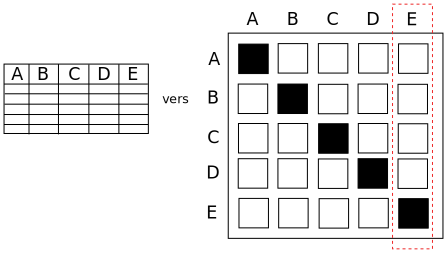
\includegraphics[width=0.6\linewidth]{matrix.pdf}
	 	\label{fig:matrice}
\end{figure}

Un algorithme évolutionnaire a été utilisé pour trouver quels étaient les valeurs minimales de valeur objectifs atteignable avec le modèle \textbf{Ants}. Autrement dit, on demande à l'algorithme d'optimisation de nous dire, dans la mesure du possible, quels sont les valeur de paramètres (génome) nous permettant de minimiser au mieux la durée (trois fonctions objectifs ${f1,f2,f3}$) pour consommer le tas de nourriture 1, 2 et 3. Au bout d'un certain nombre d'itération, cet algorithme nous propose un ensemble de solution résultats incluant le front de Pareto, existant ici en 3 dimension.

Comme il n'existe pas d'outil facile d'emploi permettant de selectionner des points dans un espace en 3 dimensions tout en affichant simultanément la valeur de paramètres auquelle chacun de ces points est rattaché, nous allons nous contenter d'un autre outil en deux dimensions. Connu sous le nom de \textit{scatterplot matrix}, celui-ci permet de représenter un ensemble de points présent sous forme tabulaire classique vers la forme de matrice, comme représenté dans la figure \ref{fig:matrice}.

Dans une forme interactive de cette représentation \Anote{scattrplot}, la selection à la souris d'un ensemble de point met automatiquement en lumière la position de ceux-ci dans l'ensemble de la matrice. Dans notre cas, à chaque point sont associé les valeurs de paramètres suivantes $(diffusion-rate,evaporation-rate, medianFood1, medianFood2, medianFood3)$ Cette représentation permet d'explorer la relation entre espace des objectifs et espaces des valeurs de paramètres en mettant tout sur le même plan. Cette exercice d'analyse, encore faisable en deux dimensions, devient un peu plus difficile à chaque fois que l'on ajoute des paramètres ou des objectifs. Afin de ne pas encombrer le chapitre par des dizaines de matrices, j'ai choisi de réunir dans un même schéma différentes selections réalisés du point de vue d'un seul axe (cf. similaire à la zone selectionné en rouge dans \ref{fig:matrice}) en prenant pour axe $x$ de référence l'objectif $f3$, le tas de nourriture à priori le plus éloigné du nid, et donc le plus difficile à minimiser.

Il ne faut pas oublier que cette analyse se fait sur une population de solution evaluée, elle est donc très ressérée autour de certains comportement clef qui détermine les contradiction auquel fait face l'algorithme d'optimisation pour minimiser ces trois objectifs à la fois. On voit bien que les écarts sont très différents selon les objectifs, ce qui peut parfois poser problème à l'optimiseur. \hl{voir un autre exemple ?}

\begin{figure}[H]
	 \centering
	 	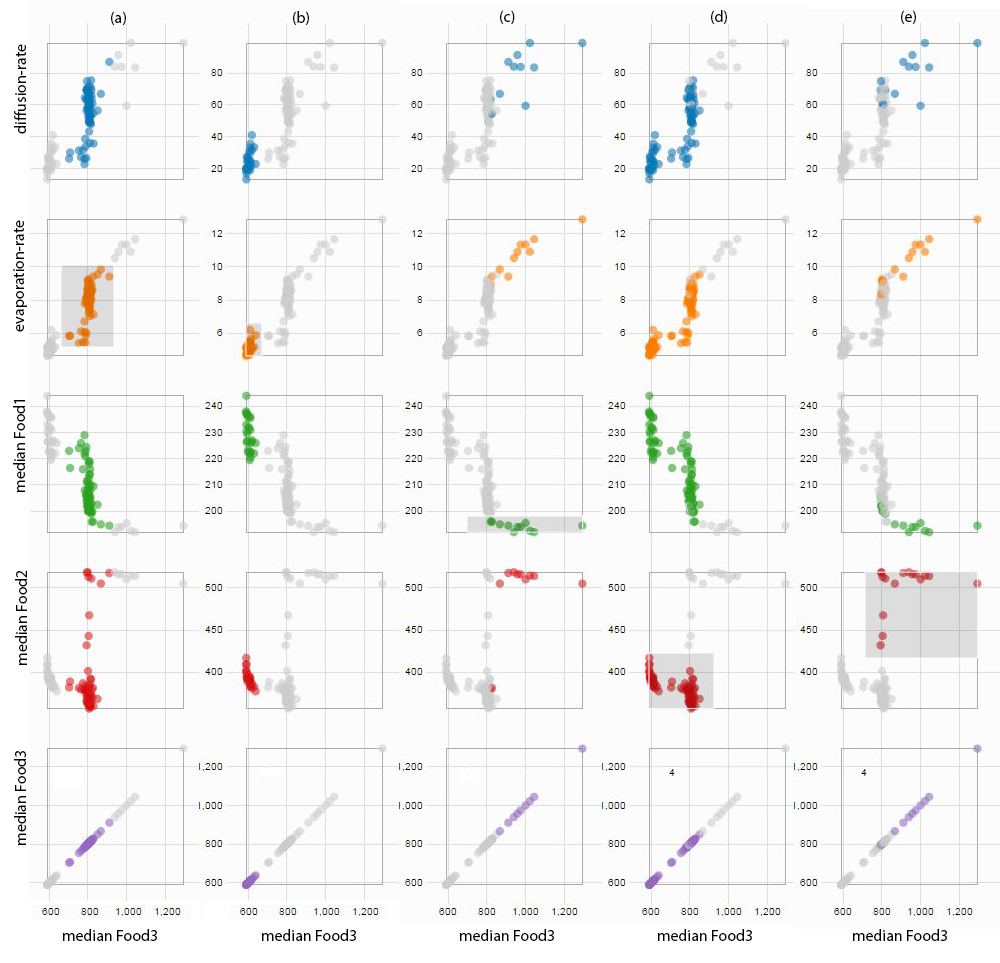
\includegraphics[width=1\linewidth]{resume.jpg}
\end{figure}

\begin{itemize}[noitemsep,nolistsep]
	\item Dans la colonne (a), on s'intéresse à un premier cluster de valeurs d'évaporation compris entre $[5.5, 10]$. On voit que pour cette selection le taux de diffusion est très étalé, entre $[20, 80]$, ce qui indique le peu d'impact de celui-ci dans cette dynamique. Quelque soit cette valeur dans cette intervale là, le modèle arrive toujours proche de valeurs égale à $800$ à +/- $100$ près pour median\textit{medianFood3}. Si il y a bien une forme de stabilité exprimé pour ce troisième objectif, le deuxième objectif est par contre beaucoup plus sensible car sa valeur peut varier de $[300, 550]$. De la même façon la valeur de l'objectif \textit{medianFood1} est très étalé entre 205 et 230. On pourrait qualifier de comportement moyen ce profil, car il ne donne pas les pires résultats sur l'objectif \textit{medianFood3}, il donne des résultats assez resséré entre $[200, 230]$ sur l'objectif \textit{medianFood1}, par contre pour l'objectif \textit{medianFood2}, c'est moins clair, il semble y'avoir un effet de seuil.
	\item On selectionne un cluster qui partage certaines valeurs avec le précédent, sur les valeurs d'évaporation comprise entre $[5, 6]$. On voit qu'avec ces valeurs là, il est possible d'atteindre des valeurs minimales sur l'objectif \textit{medianFood3}, aux environs de $600$. Pour cela la lecture de diffusion-rate nous indique qu'il faut se concentrer sur la des valeurs comprises entre $[15, 40]$. Des valeurs qui se chevauche avec la tranche donné précédemment dans la colonne (a), entre $[20, 60]$. Il semblerait donc qu'il faille voir ces deux conditions réunies, taux d'évaporation $< 6$ et taux diffusion compris entre $[20, 40]$ pour que la valeur minimale puisse etre atteinte sur l'objectif \textit{medianFood3}. Autre remarque, dans cette configuration donné, les résultat sur l'objectif \textit{medianFood1} sont moins bon, il a donc probablement fallu faire un compromis. La valeur sur l'objectif \textit{medianFood2} est stable autour de $400$, alors dans la colonne (a) ce n'était pas le cas. Le point de tension semble donc plus être entre l'objectif \textit{medianFood1} et \textit{medianFood3}, ce qui semble assez logique vu la configuration des tas de nourriture. IL faut toutefois aussi relativiser la degradation des performances sur cet objectif \textit{medianFood1}, elles sont minimes entre (a) et (b) (entre $0$ et $50$ d'écart max avec (a)), surtout comparé au gain obtenu sur l'objectif \textit{medianFood2}, plus stable et \textit{medianFood3} moins long de $200$ vis à vis de (a). Cette configuration de paramètres parait etre la plus intéressante pour le moment, tout dépend l'importance que l'on accorde à la dégradation de performance sur l'ojectif \textit{medianFood1}.
	\item La colonne (c) montre a toute évidence que les candidats les meilleurs sur l'objectif \textit{medianFood1} $< 200$, sont aussi potentiellement les plus mauvais sur l'objectif \textit{medianFood2} et \textit{medianFood3}. Plus on va vers l'intervale $[80, 100]$ sur la diffusion, et au delà de 10 sur evaporation-rate, et plus les résultats sur l'objectif \textit{medianFood2} et \textit{medianFood3} se dégrade. Toutefois par recoupement avec ce que l'on a vu dans la colonne (a), il semblerait qu'un point se détache du lot dans ce paquet, et permette d'avoir proche de $800$ à coup sur l'objectif \textit{medianFood3}, au environ de $350$ sur l'objectif \textit{medianFood2}, et $ < 200$ sur l'objectif \textit{medianFood1}. Toutefois, et c'était quelque chose que l'on avait déjà percu dans le (a), l'objectif \textit{medianFood2} a l'air assez sensible sur l'un ou l'autre de ces intervales (passe de $350$ à $500$). Cela constitue un autre jeu de valeur de paramètre intéressant, si on n'est pas pret à sacrifier sur la performance de l'objectif \textit{medianFood1}.
	\item La colonne (d) s'intéresse au groupe de valeurs $[300, 400]$ sur l'objectif  \textit{medianFood2}, on voit que selection recoupe clairement ce que l'on a vu dans les colonne (a) et (b). Si on veut obtenir une valeur pour l'objectif \textit{medianFood3} entre $[600, 800]$, et une valeur aux alentour de $400$ pour l'objectif \textit{medianFood2}, il suffit de prendre une valeur aux hasard dans cet intervale compris entre $[15, 80]$  pour la diffusion, et $[5, 10]$ pour l'évaporation.
\end{itemize}

\end{framewithtitle}

% Ou introduire la notion d'individu ?

\begin{figure}[!ht]
	\begin{sidecaption}[fortoc]{Résumé simplifié du déroulement d'une optimisation selon \textcite[109]{Weise2011}}[fig:resume_opti]
		\centering
		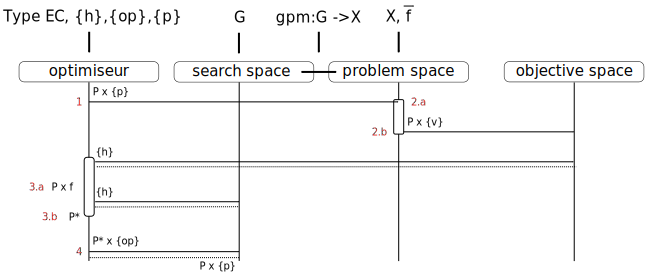
\includegraphics[width=\linewidth]{espace_resume.pdf}{
		}
  \end{sidecaption}
\end{figure}

La description des étapes de la figure résumé \ref{fig:resume_opti} sont les suivantes :

\begin{itemize}[label=\textbullet]
	\litem{1} Une première population $P \in {1 \dotsc n}$ de vecteurs paramètres ${p}$ est générée par l'optimiseur ou introduite par l'expérimentateur, puis soumis à évaluation.
	\litem{2.a} La fonction à optimiser est évaluée autant de fois qu'il y a de vecteurs ${p}$
	\litem{2.b} Les fonctions objectifs $\vec{f}$ sont calculés, ce qui permet de créer autant de vecteur ${v}$ correspond au résultats des fonctions qu'il y a de $P$ évalué. Ces vecteurs $P(v)$ peuvent être positionné dans un espace des objectif $\mathbb{Y}$
	\litem{3.a} Le calcul de fitness $f$ est effectué pour chaque élément de $P$ en utilisant les informations rapportés par un ensemble d'heuristiques sur $\mathbb{Y}$ et, ou $\mathbb{G}$
	\litem{3.b} A partir du calcul de cette fitness $f$ pour chacun des éléments de $P$, on selectionne les $P^*$ meilleurs éléments.
	\litem{4} A partir d'un ensemble d'opérateur ${op}$ on va générer de nouveaux vecteurs de paramètres $P(p)$, qui va constituer le nouveau jeu de solution candidates à évaluer à l'étape (1), et dont on espère qu'elles seront si possible meilleures que les précédentes.
\end{itemize}












\hl{Manque la notion d'invididu = fitness + genotype + phenotype}

% Injection de connaissance se fait un peu partout pour la construction d'une fitness.

% Penser à dire qu'il y a plusieurs stratégies de comparaison autre que Pareto ?

%Première fois utilisé en 1989

%Si on transfère ce langage neutre au vocabulaire que l'on peut trouver courrament dans l'EC, alors l'espace des solution devient le \textit{phenome}, et le point de cet espace qui correspond à la solution candidate devient un \textit{phenotype}.

%\begin{figure}
%\begin{sidecaption}[fortoc]{ POM cycle for developping theory for an agent behavior \autocite[245]{Railsback2012}}[fig:S_syntheseGrim]
%  \centering
% 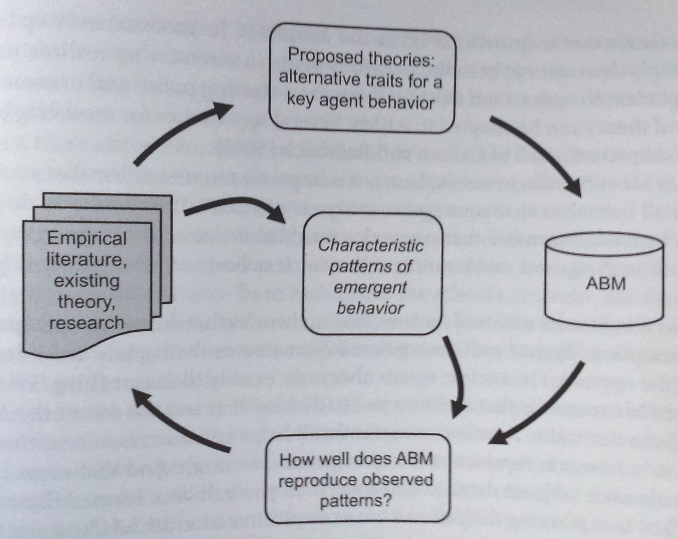
\includegraphics[width=.9\linewidth]{cyclePOMcomportement.png}
%  \end{sidecaption}
%\end{figure}


%Dans notre étude, l'objet à optimiser ne se réfère pas à une expression mathématique, mais à un modèle de simulation, sur lequel on va déterminer un ensemble de critères qui vont faire figure d'équivalent de ces fonction objectives. Dans ce cas d'utilisation, l'optimisation est plus souvent employé comme une forme de calibration inversé \autocite{Grimm2011}, dans laquelle on cherche à déterminer si il existe un ou plusieurs jeu de valeur de paramètres du modèles de simulation respectant la plage de valeur viable empiriquement qui permettent de maximiser l'obtention d'un ou de plusieurs critères experts. Il est plus parlant dans notre cas de désigner l'espace de recherche comme l'espace des paramètres.

La branche des métaheuristiques EC que nous allons étudier plus spécifiquement s'appuie sur l'observation de phénomènes naturels, comme l'évolution, ou l'organisation, pour la construction et la mise en oeuvre d'algorithmes mimant certaines propriétés intéressantes de ces processus, cela sans être rattaché à une contrainte de réalisme biologique.

\subsection{Les métaheuristiques bio-inspirées, la branche des Algorithmes Evolutionnaires}
\label{ssec:EA}

\subsubsection{Un rapide historique de la discipline}
\label{sssec:historique_EA}

On a déjà rapidement décrit dans la section à propos de l'Artificial Life \ref{p:heritage_complexe} les deux voies qu'il était possible d'emprunter dans l'intéret porté sur la définition du processus naturel d'évolution.

Il existe en effet au moins deux façons aujourd'hui d'introduire des développements informatiques se rapportant à ce processus évolutif. D'un côté, les tentatives de reproduction plus ou moins fidèles des différents mécanismes à l'oeuvre dans le processus d'évolution mettent en avant un objectif de compréhension, alors que la focalisation sur ces mêmes mécanismes pour leur seule capacité d'apprentissage tend à s'éloigner de la réalité biologique pour s'orienter plus vers le développement d'algorithmes désignés comme métaheuristiques. Autrement dit, là ou des chercheurs vont tenter de reproduire au mieux le processus d'évolution dans ce qu'il a de créatif, de non optimisé, de coévolutif car construit par \Anote{note_pattee_semantic_closure} et avec l'environnement, d'autres vont reprendre ce même processus en vue d'une évolution si possible bornée et dirigée par la résolution efficace d'un ou de plusieurs objectifs définis de façon fixe et extrinsèque \autocites{Taylor2001, Taylor2012}.

Lorsqu'on s'intéresse de plus près à la littérature scientifique de ces algorithmes regroupés depuis Fogel sous le terme d'\foreignquote{english}{Evolutionary Computation} (EC), on constate pour toute une partie des publications une de-contextualisation complète de leur utilisation. La question d'une similitude initiale avec le vivant n'étant le plus souvent évoquée que pour illustrer des racines historiques éloignées, alors qu'une meilleure connaissance de cette histoire pourrait au mieux participer d'une amélioration des algorithmes, et au pire au moins éviter la persistance de certains malentendus \autocite{DeJong1993a}. Ce qui peut apparaitre comme une forme de surspécialisation est en quelque sorte le prix à payer d'une évolution de la discipline avant tout dirigée par une communauté de chercheurs informatiques motivés par la recherche d'algorithmes performants et d'applications génériques.

Si aujourd'hui on peut observer un tel cloisonnement, un regard sur l'histoire de la discipline tend à montrer tout l'inverse, car nombreux sont les pionniers ayant développé des intérêts simultanés pour ces deux approches : les expériences très longtemps restées inconnue du mathématicien Barricelli dès 1954 \Anote{barricelli_multi_utilisation}, l'approche du généticien \textcite{Fraser1957} qui décrit et simule l'évolution de population génétique dès 1957 \Anote{fraser_comment}, les travaux de Pattee et Conrad avec EVOLVE à la fin des années 1960 \autocite{Conrad1970}, les algorithmes génétiques \Anote{holland_multi_utilisation} de Holland, un élève de Burks, un scientifique dont on a déjà vu dans le paragraphe \ref{p:va_automate_cellulaire} qu'il était proche de Von Neumman.

Il existe toutefois une littérature scientifique parallèle qui continue de motiver la rencontre autour de disciplines scientifiques ayant un intérêt pour la recherche en \textit{Artificial Life}. C'est le cas par exemple de la biologie, ou de l'écologie \autocite{Hamblin2013} qui organisent autour de publications transverses la réflexion sur la reintroduction des outils tel qu'ils sont développés en informatique, entrainant de fait aussi la création et l'évolution de ces derniers \autocite{Hogeweg2011}. C'est également le cas en biologie, ou on imagine l'importance que peuvent avoir les travaux de \textcites{Taylor2001}[221]{Taylor1999} pour la mise en oeuvre de modèles de simulation dirigés vers l'émergence \enquote{créative} de nouveaux phénotypes dans un environnement ouvert \autocite[33]{Taylor1999}. Une critique récurrente adressée aux modèles d'auto-organisation actuels \autocite{Pumain2003}, encore incapables de simuler l'émergence de nouvelles structures, de nouvelles entités de façon crédible. Une autre forme de relation entre les deux approches est également envisageable dans certaines disciplines, comme en écologie, où celles-ci peuvent parfaitement se côtoyer : \foreignquote{english}{The first of these requires the application of the evolutionary process in much the same way as it has been traditionally applied within A-Life: as a means to dynamically adjust agent parameter values to support their viability and reproduction within the virtual environment. [...] The second approach we suggest employs artificial evolution to match simulation patterns against data gathered from the level of specific species up to data concerning specific ecosystems. Once the parameters of the system have been optimised so as to reproduce the patterns observed in field data, the evolution algorithm is turned off. The model may then be employed to answer questions relating to the specific ecosystem and species that it represents. Unfortunately it may not then be used to study the evolution of these specific species in specific environments. This is a shortcoming of the artificial evolution algorithm (it does not model real evolution in detail) that would be worth overcoming.} \autocite{Dorin2008}

Le lecteur souhaitant obtenir une vue plus globale des différents concepts et ramifications disciplinaires réunit sous le terme parapluie d'\textit{Artificial Life} peuvent se référer à l'article d'\textcite{Aguilar2014} qui concentre un grand nombre d'entrées bibliographiques essentielles pour aborder les entrées de cette thématique dans chacune des disciplines. On trouvera également une description plus précise sur l'histoire commune de ces deux voies de recherches, telles quelle est perçues par les acteurs historiques de l'EC, dans les ouvrages de \autocites{DeJong2006a, Fogel1998, Fogel2006a, Fogel2006b, Back1996, Back1997}.

Dans cette section, c'est bien la deuxième branche de recherche qui est suivie, celle visant l'\enquote{optimisation}. Les développements tels qu'ils sont abordés ne se mesurent donc plus en fonction d'un critère de réalisme biologique, mais en fonction de critères informatiques et mathématiques se rapportant plus à la capacité de résolution des algorithmes, et aux supports de mise en oeuvre et de mesure de ces derniers : rapidité, diversité, robustesse, qualité, etc.

\textcite{DeJong2006a} retient trois foyers importants pour le développement de cette deuxième branche dans les années 1960, la \textit{Technical University} de Berlin avec Rechenberg, Biernet et Schwefel \autocite{Beyer2002}, UCLA à la même période avec Lawrence J. Fogel, et l'université du Michigan avec John Holland.

De ces trois branches vont émerger au cours des années 1970 ce que \textcite{DeJong2006a} qualifie comme des \foreignquote{english}{Evolutionary Algorithms (EA)} canoniques. Autrement dit, ce sont des algorithmes matures, qui ont prouvé leur capacité à produire des solutions dans un contexte précis : \foreignquote{english}{Evolutionary Programming (EP)}, \foreignquote{english}{Evolution Strategy (ES)}, \foreignquote{english}{Genetic Algorithm (GA)}

Ils vont représenter chacun le foyer d'un développement qui va s'accélérer dans les années 1980, avec l'amorce d'une popularisation de ces techniques permises entre autres par l'avènement de capacités de calcul plus conséquentes et la reconnaissance de l'efficacité de ces algorithmes pour la résolution de problématiques industrielles plus concrètes. L'ouvrage de synthèse écrit par \textcite{Goldberg1989} contribue de façon très importante à cette diffusion, et constitue également un apport théorique important dans la naissance de la branche multi-objectif de cette discipline.

Les années 1990 vont quant à elles consacrer la rencontre et l'unification de ces différentes approches restée jusqu'alors assez indépendantes si on en croit \textcite{DeJong2006a}. De cette confrontation nait la reconnaissance d'un seul terme fédérateur, l'\textit{Evolutionary Computation (EC)} motivant alors la création de nouvelles conférences et de nouveaux journaux structurant cette nouvelle discipline. C'est aussi à partir de cette période que l'on observe la mise en place d'une hybridation accélérée entre les différentes approches qui s'accompagne d'une forme de remise à plat théorique et l'émergence d'un cadre de réflexion unifié. \autocites[23-31]{DeJong2006a}{Back1997}

Si on se concentre plus précisément sur la branche multi-objectif de la discipline, la première introduction théorique d'une stratégie s'appuyant sur le calcul de l'optimum de Pareto pour définir un classement original des solutions évalués est présenté à la page 197 de \textcite[197]{Goldberg1989}. Cette technique nommé \textit{Non Dominated Sorting} (NDS) \autocite[40-43]{Deb2001}, probablement la plus efficace et plus célèbre, sera reprise et implémenté presque dix ans plus tard en 1994, dans l'algorithme célèbre NSGA (Non dominated Sorting Algorithm) de Deb et Srinivas.

Les travaux de \textcite{Goldberg1989} ont influencé tout une génération de chercheurs à partir de cette simple ébauche théorique de tri basé sur la dominance de Pareto, et nombreux sont ceux qui se sont par la suite appuyés \autocite[175, 235]{Deb2001} sur les informations du calcul de dominance pour développer diverses stratégies d'attribution de \textit{fitness}, comme MOGA (Fonseca et Flemings 1993 \autocite{Fonseca1993}), NPGA (Horn et Nafpliotis 1994), NSGA (Deb et Srinivas 1994), et bien d'autres \autocite[14]{Zitzler1999a}. Ce que l'on peut considérer comme la génération suivante d'algorithmes, que \textcite{Coello2006} \Anote{coello_note} fait démarrer avec l'apparition de l'élitisme \Anote{note_elitisme}, est plus axée encore sur l'efficacité de ces derniers avec notamment l'ouverture d'une branche de recherche développant des métriques de performance, et de nouveaux standards de mesures \autocites{Coello2006, Zitzler2003,Huband2006}, dont on s'aperçoit qu'elles sont devenues nécessaires pour comparer correctement les algorithmes entre eux \autocite[14-15]{Zitzler1999a}. Parmi ces nouveaux algorithmes, devenus depuis canonique, on trouve PAES (Knwoles and Corne 2000), SPEA (\autocite{Zitzler1999}), ou encore NSGA 2 (Deb 2000) etc. On trouve à ce sujet un état de l'art et des exemples de calculs à la main pour ces différents algorithmes dans un des premiers et très bon ouvrage de synthèse de \textcite{Deb2001}, aux chapitres 5 et 6. Il est toutefois à noter, comme le fait déjà Golberg en 1989, que cette problématique de recherche d'une solution à un problème multi-critères, puis multi-objectifs est d'origine bien plus ancienne, et a pu servir de support à la mise en oeuvre de techniques plus ou moins similaire à celle de Pareto. Ainsi, les premières traces en EA d'un intérêt théorique et parfois pratique de ces problèmes semblent remonter à Box et Draper (1957), Fogel (1966), Rosenberg (1967) \autocite[174-175]{Deb2001}. Mais la première implémentation informatique est en général attribuée à David Schaffer, avec son travail de thèse (1984) et l'implémentation de l'algorithme d'optimisation VEGA (\textit{Vector Evaluated Genetic Algorithm}) \autocite{Schaffer1985}. Un autre état de l'art sur l'optimisation multi-objectifs s'appuyant sur Pareto en dehors des techniques purement évolutionnaire est également possible. C'est grâce à l'existence de ce cadre formel mathématique permettant la description d'un problème d'optimisation, tel que nous l'avons un peu abordé dans la section précédente en s'appuyant sur les écrits de \autocite{Weise2011}, que \textcite[50-79]{Deb2001} indique par exemple comment certaines de ces stratégies hors EC ont été pour certaine également transférées avec plus ou moins de succès aux EA \textcite[171-237]{Deb2001}.

Enfin on notera qu'il existe également une autre classe proche d'algorithmes d'optimisation basée sur une observation des mécanismes naturels, celle-ci n'étant plus basée sur la métaphore évolutive par reproduction (même si l'hybridation est envisageable), mais sur les capacités d'organisation et d'auto-organisation observées chez certains animaux comme les fourmis, les abeilles. Ces comportements ont d'abord inspiré les développements de plateformes informatiques adaptées à l'émergence de ce type de comportements, avant d'être repris et utilisé de façon beaucoup plus abstraites par la suite pour résoudre des problèmes d'optimisation. Aujourd'hui regroupées sous le terme de \foreignquote{english}{Swarm Intelligence}, ce sont par exemple les algorithmes PSO (Particle Swarm Optimization), ACO (Ant Colony Algorithms), ABC (Artificial Bee Colony), etc.

\subsubsection{Les principes sous-jacent aux EA}
\label{ssec:principesEA}

Afin de pouvoir mettre en oeuvre la possibilité d'une telle souplesse dans l'adaptation de l'algorithme à une problématique d'optimisation donnée, \textcite[49]{DeJong2006a} a considéré la construction d'un modèle conceptuel plus abstrait capable d'englober dans sa description les mécanismes d'au moins ces trois version canoniques GA, ES et EP. Les concepts clef qui se dégagent d'une telle prise de distance peuvent ainsi être repris non seulement pour décrire les version canoniques mais également pour développer de nouvelles variantes ou extensions d'algorithmes.

Les éléments communs retenues sont les suivants :

\begin{itemize}
\item Une population de taille constante $m$ évolue au cours du temps
\item La population courante est utilisée comme une source de parents pour produire une progéniture (\textit{offsprings}) de taille $n$
\item La population étendue ainsi constitué est réduites de $m + n$ à $m$ individus.
\end{itemize}

\hl{a completer avec schéma expliquant les différentes etapes de l'algorithme générique en EA}

% En général puis recentrage sur les détails ?
\paragraph{Les avantages et les inconvénients d'une terminologie spécifique}

En 2014 une publication sur le blog du spécialiste de la discipline Thomas Weise's \Anote{billet_weise} revient longuemment sur les problématiques de ce vocabulaire inspiré par la biologie et ancré dans les différentes branches composantes l'EC. Il retient quatre problématiques dans l'usage de cette terminologie, parmi lesquels l'incompatibilité des terminologies entre les différentes branches, la dissonance entre la terminologie et la réalité d'application des algorithmes, le fait que l'optimisation au sens naturel n'est pas forcément une bonne optimisation, le fait également que cette terminologie sonne comme anti--professionnelle \Anote{note_pengouin}. Le plus grand problème étant dans ce cadre l'invention de néologisme ne faisant référence ni au domaine biologique, ni au domaine informatique. Ce n'est pas la seule voix à se faire entendre sur ce sujet, comme l'article de \textcite{Sorensen2013b} qui pointe clairement les dérives néfastes associées à l'usage systématique et surtout non réellement argumenté de nouvelles analogies ou métaphores, que celle-ci soit biologique ou pas ...

Si la perspective d'un changement d'annotation et de vocabulaire est probablement conçue comme une étape majeure dans la progression et l'unification d'une discipline depuis quelques années déjà sur la voie de la maturité, Weise tout en prônant au maximum la bonne parole continue comme beaucoup d'autres à utiliser cette terminologie \autocite{Weise2011}, très ancrée dans un folklore qui tient à l'historique de la discipline. La librairie logicielle MGO décrite par la suite s'appuie elle aussi sur cette terminologie, aussi nous n'utiliserons donc les terminologies alternatives proposées par Weise que sous forme de complément, afin de ne pas introduire trop de distance entre les termes décrivant les algorithmes dans ce manuscrit et la réalité du programme tel qu'il est conçu pour le moment.

\begin{table}[!htbp]
\begin{sidecaption}[fortoc]{Tableau de correspondance entre les notations à consonances biologiques et les notations plus génériques liées à l'optimisation, lorsque celles-ci existent. Une traduction appuyée sur la section précédente, et les travaux de \textcite{Weise2011}}
	[tab:ptraduction]
	\centering
	\begin{tabular}{ll}
		\toprule
		générique & biologique (FR)\\
		\midrule
		Espace du problème ($\mathbb{X}$) & Phénome \\
		Espace de recherche ($\mathbb{G}$)   &  Génome \\
		Point dans un espace de recherche ($g \in \mathbb{G}$) & Génotype \\
		Solution candidate, Point dans un espace de solutions ($x \in \mathbb{X}$) & phénotype \\
		Opérateurs de recherches ($searchOp$) & Reproduction \\
		Opérateur de recherche Unaire & Mutation \\
		Opérateur de recherche Binaire & Crossover \\
		Itération & Génération \\
		?  & Progéniture \\
		?  & Mating pool \\
		\bottomrule
	\end{tabular}
  \end{sidecaption}
\end{table}

\paragraph{Les avantages et les inconvénients des EA}

Ces deux listes comparant les avantages et les inconvénients des algorithmes évolutionnaires sont tirés des ouvrages de Deb2001, Fogel2000, Back1997, \autocite[104,105]{DeJong2006a} mais également Openshaw qui a exploré ces techniques en géographie. \hl{ref a completer}

\begin{enumerate}[label=(\alph*),labelindent=\parindent,leftmargin=*]

	\item Evaluation d'une population entière par génération, ce qui n'est pas le cas de nombre de techniques fournissant une seule solution par exécution d'algorithme.
	\item Facile à paralléliser, une propriété étudiée très tôt \autocite[444]{Alba2002}
	\item Ne demande a priori aucune connaissance de la forme du paysage, même si en réalité c'est un plus pour bien choisir et paramétrer les métaheuristiques
	\item Applicable à des problèmes continus, discrets, ou les deux.
	\item Ne demande pas forcément de repartir de zéro entre chaque analyse en comparaison à d'autres algorithmes
	\item Le nombre de degrés de liberté accessible pour modifier une métaheuristique est très important, ce qui augmente les chances de trouver une combinaison adaptée à un problème complexe donné
	\item Les principes de mise en oeuvre sont relativement faciles à comprendre
    \item Efficace, même sous une forme canonique
    \item Capacité à explorer de très large espace de recherche
\end{enumerate}

Les désavantages, limitations :

\begin{enumerate}[label=(\alph*),labelindent=\parindent,leftmargin=*]
	\item le fonctionnement reste opaque, et le résultat n'est souvent pas tractable mathématiquement
	\item la stochasticité demande la mise en oeuvre de réplication
	\item pas de garantie de trouver un optimum global
	\item le nombre de degrés de liberté demande une certaine forme expertise pour en tirer le meilleur parti, la construction d'un EA optimal pour un problème donné étant progressif, incrémental
    \item trop facile à comprendre, il en résulte une certaine illusion quant aux capacités \enquote{magiques} de ce type d'algorithme.
    \item necessite une source conséquente de puissance pour réaliser de grands nombres de calculs en parallèle
    \item les performances se dégrade avec l'augmentation de l'espace de recherche (dimensionnalité) ou le nombre d'objectifs (on touche les limites de l'approche Pareto) \hl{ref Zitzler1999a page 24 cite Fonseca Flemming 1995}
\end{enumerate}

\hl{2 paragraphe qui suivent à replacer au bon endroit}

L'optimisation de paramètres est un domaine d'application reconnu des EA du fait aussi de la facilité de mapping entre vecteur de paramètres et génome \autocite[83]{DeJong2006a}

Dans la lignée des objectifs définis dans le chapitre 3, cette branche spécifique des EA est celle qui est à la fois la facile d'accès en terme de compréhension pour les débutants tout en restant également suffisament flexible et efficace pour convenir à notre utilisation.

De plus certains désavantages sont de conséquences plus limitées dans le cadre de nos objectifs. En effet, pour le profil d'utilisateur modélisateur que nous visons la garantie d'un optimum global n'est pas la priorité immédiate en comparaison de l'importance d'accéder rapidement à des premiers résultats via un premier EA générique exécutable, qu'il pourra de toute façon ensuite améliorer du fait de la nature métaheuristique de ces algorithmes. De façon similaire, le fait que le résultat ne soit pas tractable mathématiquement n'est pas vraiment problématique dans le cadre des systèmes complexes, ou ce type d'observation est justement une propriété récurrente des systèmes que l'on cherche à simuler pour mieux les comprendre.

Enfin, il est important de noter que cette classe d'algorithmes accueille les approches les plus efficaces pour la résolution de problèmes multi-objectifs, une propriété courante des problèmes abordés dans notre discipline, car les modèles de simulation construisent souvent leur crédibilité aux croisements de multiples critères. (\hl{POM, cf problème inverse calibration déjà expliqué en chapitre 3?})

\hl{Introduction à un algorithme simplifié, soit sous forme d'algorithme, soit sous forme de schéma}

% \begin{algorithm}[H]
%  \KwData{this text}
%  \KwResult{how to write algorithm with \LaTeX2e }
%  initialization\;
%  \While{not at end of this document}{
%   read current\;
%   \eIf{understand}{
%    go to next section\;
%    current section becomes this one\;
%    }{
%    go back to the beginning of current section\;
%   }
%  }
%  \caption{How to write algorithms}
% \end{algorithm}

%Chacun de ces items ouvre quasiment la voie à des sous-domaines d'expertises spécifiques.
Voici un aperçu cumulatif des élements susceptibles de varier d'un algorithme à un autre, et d'une application à une autre, dont certain sont hérités de la nature métaheuristique des EC, puis de la nature spécifique des EA, et enfin de la nature multi-objectifs (*) : \autocite[69,72,115]{DeJong2006a}[264-269]{Weise2011}[91]{Liefooghe2010} :

\begin{itemize}
\item la stratégie de représentation interne d'une solution
\item la stratégie d'initialisation et de maintien d'une ou de plusieurs populations
\item les stratégies de sélection des parents pour la reproduction
\item les stratégies de réintroduction des enfants dans la ou les population(s)
\item le groupe d'opérateurs choisi et la stratégie d'utilisation de ces opérateurs dans le processus de reproduction
\item le choix d'une fonction de translation \textit{gpm} entre $\mathbb{G}$ et $\mathbb{X}$
\item (*) les stratégies de préservation de la diversité
\item (*) les stratégies élitistes de sélection et de maintien des survivants
\item (*) la méthode d'attribution d'une \textit{fitness} $v$
\item le critère d'arrêt
\end{itemize}

Si cette liste de classe de choix permet de cerner de façon plus globale les questions à se poser lorsqu'on construit ce type d'algorithmes, cette représentation est encore trop vague, trop linéaire, et ne rend pas compte de la plasticité et des contraintes voulues ou imposées par la construction dynamique d'un algorithme véritablement adapté au problème. Les dépendances entre éléments de la liste n'apparaissent pas dans cette représentation, or pour chacun des choix réalisés par l'expérimentateur a lieu un recalcul des degrés de liberté, ce qui entraine l'apparition ou la disparition de nouveaux choix, en fonction des dépendances existantes entre chaque élément. \Anote{reflexion_DeJong}

Par exemple, le choix d'une représentation interne d'une solution sous forme de vecteur de binaire, réel ou encore mixte, de taille dynamique ou fixe, doublé ou non de paramètres spécifiques de convergence, joue de façon assez logique sur les choix disponibles dans chacune de ces classes. Ainsi le groupe d'opérateurs choisis pour manipuler ces vecteurs lors de la reproduction des individus ne seront pas les mêmes selon qu'on manipule des éléments Binaires ou Réels.

De plus, il faut imaginer que chaque stratégie est accompagnée de son lot de paramètres associés, et ce n'est qu'à terme d'une construction, lorsque le choix d'une combinaison d'éléments est actée, que la liste de paramètres définitive de la métaheuristique apparait de façon claire à l'expérimentateur.

Enfin, dans notre cas, où il est question d'utiliser ces algorithmes évolutionnaires en s'appuyant sur toute la puissance informatique disponible, de nombreux nouveaux choix \autocite[221-224]{DeJong2006a} émergent à la lumière des modèles plus poussés de parallélisation des EA. Par exemple la mise en place d'une stratégie de parallélisation en ilôts de population, dont on verra un peu plus loin qu'elle est optimale pour une utilisation des métaheuristiques sur une grille de calcul, pose les nouvelles questions suivantes :

\begin{itemize}
	\item quelles sont les stratégies de migration des individus entre les différentes populations ?
	\item combien d'ilots sont nécessaires ?
	\item les populations initiales de chaque ilot sont elles identiques ou différentes ?
	\item quelle topologie d'ilot est la plus adaptée ?
	\item etc.
\end{itemize}

C'est un aperçu des problèmes que nous tenterons de résoudre avec la construction d'une librairie logicielle à l'architecture originale, couplé avec openMOLE pour gérer la partie parallélisation, et qui sera exposé dans les sections suivantes.

Une partie de la modularité inhérente aux métaheuristiques a déjà pu par chance être saisie dans le développement de nombreuses librairies logicielles, il est alors légitime de se poser la question suivante, \textit{pourquoi développer et surtout maintenir une nouvelle librairie ? }

Les raisons de ce choix sont guidées par une observation critique des librairies existantes, réalisée un peu plus loin dans cette section, et la volonté de satisfaire au mieux les critères évoqués dans le chapitre 3 \hl{ref section}.

%\paragraph{Expression au niveau de l'expérimentation : }

%\begin{enumerate}

%\item{Besoin de plus de flexibilité ?}

%\end{enumerate}

% Faire un rapel vers la grille.
% MODYSS !

\paragraph{Au niveau utilisateur, cas d'utilisation orienté vers les métaheuristiques}

MGO devra être supporté par une architecture qui répond aux exigences différentes d'un public novice et expert, ce qui suppose une analyse de la possible évolution des besoins.

\hl{a developper} Qu'est ce qui fait la facilité de prise en main ? Respecter les pratiques existantes, tout en offrant des solutions alternatives dès que le modélisateur en ressent le besoin, si possible à moindre coût.

\begin{enumerate}
	\item{\textbf{Besoin de plus de flexibilité ?}} L'algorithme évolutionnaire proposé en l'état (canonique) ne donne pas de bons résultats, le programme doit permettre d'accéder \textbf{facilement} à toute la combinatoire offerte par la variation des différents composants intégrant cette branche des métaheuristiques.

	\item{\textbf{Besoin de plus de puissance ?}} Fonctionnel sur une machine standard, les algorithmes évolutionnaires doivent pouvoir tirer parti de ressource informatique plus importante de façon locale (multi-coeur) ou distribuée (cluster, grille de calcul), et cela en utilisant les méthodes adaptées. Ce passage d'une exécution locale à une exécution distribué doit être possible le plus \textbf{facilement} possible.

	\item{\textbf{Besoin de plus d'extensibilité ?}} Je ne trouve pas le composant nécessaire à la construction d'une métaheuristique adaptée à mon problème, quels sont les outils mis à ma disposition pour que je puisse ajouter le ou les composants facilement, à moindre cout, sans que l'ensemble du programme ne soit affecté par mes modifications ?
\end{enumerate}

En résumé, Mgo doit assurer \hl{repetition ici, a revoir} :

\begin{itemize}
	\item La mise à disposition d'une collection d'algorithmes évolutionnaire mono et multi-objectifs, directement utilisable
	\item mais également extensible et modifiable car décrit dans une syntaxe lisible exposant la structure interne en partie modulaire de ces métaheuristique.
	\item Une prise en charge automatique et transparente des architecture multi-coeur locale ou distribué
\end{itemize}

Mais si on se contente d'évoquer seulement ces objectifs-là, on reste dans une construction isolée dont il faut encore l'interfacer, la relier, à l'exécution de nos modèles de simulation. Ce qui suppose d'un point de vue technique la prise en compte d'un certain nombre de problématiques techniques qui tiennent déjà en réalité d'expertises très différentes.

Un processus au coeur de l'optimisation, car c'est bien sur la base des résultats fournis par l'évaluation d'une population de modèles, devant encore être passés au crible des critères objectifs définis par les modélisateurs, que l'optimiseur va se baser pour cheminer vers des solutions quasi optimales.

\paragraph{Au niveau utilisateur, cas d'utilisation orienté vers la modélisation }

\begin{enumerate}

	\item{\textbf{Changement de simulateur ?}} Mon modèle évolue pour changer de plateforme de simulation, en passant par exemple de Netlogo à Gamma. Est-il possible de conserver mon expérience définissant l'optimisation et les paramètres de l'optimisation au cours de ce changement ? Autrement dit, changer le moteur implique-t-il le changement automatique de toute la voiture ?

	\item{\textbf{Bibliothèque d'exemples disponible ?}} Existe-t-il une bibliothèque d'expérimentations comportant un ou plusieurs exemples ou patron(s) pour une utilisation du modèle de simulation avec des métaheuristiques ?

	\item{\textbf{Liens entre logiciels de modélisation et ressources informatiques ?}} L'utilisateur doit-il réaliser lui-même la brique logicielle permettant le couplage entre le simulateur et les différents logiciels spécialisés pour utiliser des ressources informatiques distribuées ?

	\item{\textbf{Comment se définissent les expériences ?}} Existe-t-il des facilités pour décrire les plans d'expériences ? Comment le modèle est-il intégré dans une chaîne de traitement comportant une optimisation par métaheuristique ? Comment réalise-t-on le mapping entre les paramètres du modèle et la représentation interne d'une solution ? Comment décrire et transmettre les fonctions objectifs aux algorithmes pour évaluer les sorties du modèle une fois exécuté ?

	\item{\textbf{Quels supports d'interactions ?}} Est-ce que les fonctionnalités sont accessibles par une manipulation interactive dans un logiciel ou par le biais de commandes dans des scripts ?

	\item{\textbf{Quelle reproductibilité ?}} Au-delà de la simple réplication des simulations, quel niveau de reproductibilité, quelle confiance peut-on attendre d'un couplage de logiciels aussi complexe ?

\end{enumerate}

\paragraph{Au niveau institutionel, cas d'utilisation orienté vers le déploiement }

Question de la distribution des algorithmes évolutionnaires. Quel cas d'utilisation est le plus aisé à mettre en place dans des laboratoires de science humaines ?

\hl{en cours}

% Les questions à ce niveau là sont encore plus nombreuses.

% - Modulation de l'accès à la puissance informatique indépendante du modèle : Intégré à OpenMOLE, le couplage doit apparaitre comme transparent, tout en restant hautement flexible ce qui suppose l'existence de primitive de plus haut niveau qui assure la partie parallélisation nécessaire à l'usage confortable de tels algorithmes.

% - Découpler les plateformes de simulation

% - Supporter différents niveau de parallélisme au niveau des métaheuristiques

% - La facilité d'ajout de nouveaux composants

% - Une bibliothèque d'algorithmes canonique à disposition

% - La documentation

% Dans l'association entre modèle de simulation et métaheuristique : Modalités de jointure entre le modèle de simulation \enquote{tel qu'il est développé} et la librairie d'algorithme évolutionnaire.

% - Séparation entre modèle de simulation
% -

% Deux phases ?
% - Usage indépendant
% - Usage associé à openMOLE

% fait apparaitre l'optimisation comme une étape supplémentaire dans l'expérimentation,

% %BehaviorSearch follows in the tradition of NetLogo [Wilensky, 1999, 2001; Tisue & Wilensky, 2004], and Logo [Papert, 1980] before it, in embracing the twin design goals of “low threshold” and “high ceiling”. By this we mean that the BehaviorSearch tool should be both easy for beginners to learn and use (“low threshold”), while also providing advanced features that will allow expert modelers to engage in cutting-edge research and analysis (“high ceiling”). To be clear, the “low threshold” goal for NetLogo, which aims to support use by elementary school students, is lower than that of BehaviorSearch, which primarily targets NetLogo’s research audience. However, increasingly NetLogo is being used by undergraduates or even high school or middle school students who are developing agent-based models for research projects, and we would like BehaviorSearch to be accessible to these audiences, as well as researchers from various disciplines who are non-expert programmers but have adopted ABM methodologies for their research. Just as NetLogo strives to make the creation of agent-based models accessible to children and novices, BehaviorSearch aims to facilitate model analysis by making search and optimization techniques accessible to all modelers.

% State of the Art
% Flexibilité

% Facilité de parallélisation
% Facilité de construction

\subsection{Un point rapide sur les solutions EC existantes}
\label{ssec:EC_existantes}

Les librairies logicielles permettant la mise en oeuvre d'algorithmes évolutionnaires existent dans de très nombreux langages informatiques. Les \textit{Survey} ou \textit{state of the art} sont régulièrement mis à jour dans cette discipline, et il est inutile de se substituer ici à ce type de travaux en évoquant les avantages et les inconvénients comparés de toutes ces librairies. Le lecteur pourra se référer à l'étude très complète de \textcite{Parejo2012} comparant selon 271 critères 11 des plus importantes plateformes sur les 33 qu'ils ont identifiés. On se contentera ici d'illustrer ce que l'on considère comme les principaux défauts du point de vue de notre grille de lecture en sélectionnant pour cette critique une ou plusieurs librairies parmis les plus usitées.

Un premier filtre permet d'éliminer toute celle qui ne s'adresse qu'à une seule branche des EA, ou qui n'implémente aucun des algorithmes multi-objectifs.

Un deuxième filtre permet d'éliminer également toutes les librairies qui sont intégrées à un logiciel, donc impossibles à utiliser en dehors de celui-ci. Le cas particulier des logiciels de modélisations (simulateurs) intégrant des algorithmes EC sera tout de même abordé dans la section suivante afin de situer les limites de ces approches. Comme la librairie logicielle réalisée doit être compatible a minima avec plusieurs logiciels de modélisations existants, il ne parait pas intéressant de partir vers une solution se basant sur l'extension de ces derniers.

Afin de satisfaire les objectifs que nous avons fixés, la librairie doit pouvoir fonctionner avec OpenMOLE, car une des tâches de ce dernier va être d'orchestrer de façon transparente la parallélisation de ces algorithmes évolutionnaires, ce qui suppose une interaction assez fine entre les deux outils, et un langage informatique compatible avec Java ou Scala, les deux langages sur lesquels est construit OpenMOLE.

\subsubsection{Les approches intégrées}
\label{sssec:approche_integree}

\paragraph{Les tentatives isolées}

Openshaw Diplock,
Hepenstall et al,
etc.

\hl{en cours}

\paragraph{Le {BehaviorSearch} de Stonedahl}

La librairie \textit{BehaviorSearch} développée par Railsback pour Netlogo intègre une librairie d'algorithme génétique.

Les solutions existantes de couplage, comme le \textit{behavior search} déjà évoqué dans \hl{la section XX} ne sont pas entièrement satisfaisantes, cela sur plusieurs points déjà évoqués et résumés ci-dessous, auxquels on rajoute de nouveaux inconvénients propres à la manipulation avancé des métaheuristiques :

a) Le cycle de vie d'un modèle ne se limite pas forcément à l'établissement d'un seul modèle Netlogo, mais plusieurs, et de complexité différente. Si Netlogo est un outil indispensable de par la force et la rapidité de concrétisation d'une idée scientifique qu'il permet, les scientifiques auto-didacte peuvent rapidement être piégés par des problématiques tenant plus de la \enquote{science informatique} que de leur domaine initial.

b) Le niveau de prise en charge de l'expérimentation est insuffisant pour assurer une recherche reproductible au-delà du seul modèle. Par là il faut comprendre que le protocole scientifique supportant l'évaluation du modèle de simulation n'est pas accessible, or tout comme le modèle, celui-ci possède sa propre voie de construction, et porte au contact du premier une responsabilité dans l'évolution des choix de sa structure interne. Autrement dit, sans la présence de ces deux supports de connaissances, c'est toute une discussion collective qui est rendue plus complexe, alors même que celle-ci se révèle comme un support important, voire même constitutive de ce processus de validation.

c) Le support du parallélisme implicite à ce type de métaheuristique EC en local, c'est-à-dire sur un ordinateur personnel, même lorsqu'il est associé à des techniques pour réduire le nombre d'exécutions des modèles de simulation (en utilisant par exemple du \textit{fitness caching} \autocite[245]{Stonedahl2011a}), ne semble pas suffisants pour une utilisation confortable et répétée d'algorithmes métaheuristiques multi-objectifs. Ces derniers pouvant demander pour des modèles relativement simples et optimisés jusqu'à plusieurs millions d'executions, résultat d'une accumulation d'expérimentation nécessaire pour la construction et l'évaluation du modèle de simulation \autocites{Schmitt2014, Cottineau2014b}. Le framework théorique QBME (\textit{Query-Based Model Exploration}) de Stonedhal est intéressant, et ressemble par certains aspects à la méthodologie POM de Grimm, et permet comme dans cette dernière de questionner la progression du modèle sous la forme d'une question inversée par rapport au questionnement plus traditionnel. On ne se demande plus \enquote{Quels comportements vais je obtenir avec ce jeu de paramètres} mais plutôt \enquote{Quels types de paramètres m'a permis d'obtenir (ou de ne pas obtenir) un certain comportement ?}. Ce type d'analyse se base sur la construction de multiples critères d'évaluation, potentiellement contradictoire, questionnant la dynamique du modèle, et qui il me semble, se rattache plus à l'expression d'une analyse multi-objectifs. Or, les algorithmes proposés par le \textit{BehaviorSearch} se limitent pour le moment à des algorithmes mono-objectif que les cas d'utilisation réels risquent de très rapidement mettre en défaut.

d) Le support ne permet pas à l'heure actuelle de jouer \enquote{facilement} avec les briques mises à disposition par les métaheuristiques, ce qui on l'a vu précédemment va à l'encontre de l'esprit de tels algorithmes. Même si une certaine extensibilité du logiciel a été prévu par le concepteur, sa mise en oeuvre demande des connaissances supplémentaires dans un autre langage de programmation que Netlogo (Scala ou Java), ce qui vient encore surcharger un peu plus les prérequis d'un utilisateur débutant qui doit déjà explorer le domaine des algorithmes évolutionnaires.

Même si l'auteur est effectivement d'accord avec le concepteur du \textit{BehaviorSearch} pour dire que cet outil constitue en lui même déjà un grand pas vers la démocratisation de techniques d'expérimentation plus évoluées jugées nécessaire pour améliorer les pratiques des débutants, nous pensons qu'il est possible d'aller encore beaucoup plus loin. A ce titre, le couplage que nous visons dans ce projet se rapproche des visions d'avenir évoqués par le concepteur, dont la dernière version du logiciel est daté de 2013 \textcite[295]{Stonedahl2011a} \foreignquote{english}{In the not-so-distant future I envision in a “begin parallel search” button appearing in toolkits like NetLogo that would seamlessly launch dozens or hundreds of simultaneous genetic algorithms searches on a remote grid/cluster, reporting back the most promising results to the user as they are discovered in real-time.} La différence c'est que ce bouton n'est pas envisagé dans Netlogo, car ce n'est pas le propre de cet outil, mais dans un logiciel tel qu'openMOLE, dont la fonction est entièrement dédié à l'exécution de tâche en parallèle sur des environnements locaux (un ou plusieurs processus d'une machine), ou distribués (sur une grille de calcul, ou un cluster d'université)

Si on envisage en effet la construction de modèles sur la base d'une alternance régulière entre construction de modèle et évaluation, il est tout à fait possible et même certain que l'expérimentateur soit un jour ou l'autre confronté à une ou plusieurs limitations provenant de la chaine de progression naturelle prévue par les concepteurs de cet outil \foreignquote{english}{Netlogo(for building the model) => Behavior Space (for simple model analysis) => BehaviorSearch (for more advanced analysis and exploration)} \autocite[340]{Stonedahl2011a} ? Quels sont les choix à disposition des modélisateurs débutants ayant expérimenté l'une ou l'autre de ces difficultés ? (\hl{A voir si cela ne remonte pas dans le chapitre 3 pour clôturer la partie netlogo})

En résumé, les librairies déjà intégrées au logiciel de modélisation, comme le \textit{BehaviorSearch} de Netlogo, sont limitées en termes d'algorithmes, d'accès la puissance informatique nécessaire, et reste liées à un seul et unique support alors même que le modèle peut être amené à migrer de plateforme. On en déduit que cette solution, bien qu'utile pour du prototypage et de l'apprentissage, ne permet pas d'envisager sereinement la construction d'un modèle ou d'une expérimentation sur une durée plus longue.

\paragraph{Les algorithmes EC dans Mason}

Le framework de développement de simulation multi-agent MASON (\textit{Multi-Agent Simulation Of ...}) présenté pour la première fois en 2003 tient d'un effort conjoint entre la section d'\textit{Evolutionary Computation} du laboratoire de science informatique et le \textit{Center for Social Complexity} tout deux de la George Mason University. Ecrit en Java, solidement documenté, de développement ancien, associé depuis les débuts à un laboratoire spécialisé auteur d'une librairie datant de 1998 dédié aux EC nommée ECJ (1998), les deux logiciels étant développés par les mêmes personnes et régulièrement mis à jour ... ce framework apparait au premier abord comme un challenger sérieux pouvant se substituer à Netlogo sur des projets plus complexes.

MASON se situe sur la même ligne de développement que les librairies de développement multi-agents plus anciennes comme Swarm, Ascape, ou Repast. Tout comme ces dernières, la généricité, la performance et la modularité sont des composantes de l'application au coeur des préoccupations de Sean Luke, un des développeurs à l'origine du projet.

Une des spécificités très fortes de MASON, et qui rend cette librairie vraiment différente des trois autres, tient dans son histoire particulière. Si on en croit le développeur Sean Luke \Anote{sean_luke_mason}, c'est à la suite de sa thèse en 1998 et du développement de la librairie ECJ \Anote{sean_luke_ecj} dédié aux algorithmes d'EC, que celui-ci a ressenti le besoin d'une nouvelle librairie en accord avec ses problématiques de recherches en robotiques. A cette époque déjà, il utilise ECJ pour optimiser le comportement de robots opérant dans un environnement partagé, un domaine de recherche dont on a vu dans la section \hl{ref} que la simulation multi-agents était très liée historiquement. Cette pratique nécessite l'exécution de centaines de milliers de simulations, à la recherche de combinaisons de paramètres satisfaisants les critères dirigeant l'optimisation. La rapidité d'exécution d'une simulation devient un élément clef dès lors que ce sont des milliers, voire des millions de simulations qui doivent être executées en parallèle. C'est donc tout naturellement que celui-ci a initié sa propre librairie de simulation multi-agent, orienté vers l'utilisation efficiente des architectures multi-coeurs et depuis peu multi-ordinateurs (extension D-Mason). MASON étant conçu en parallèle de la librairie \href{http://cs.gmu.edu/~eclab/projects/ecj/}{@ECJ}, les deux outils fonctionnent très bien ensemble, et permettent l'exploitation de ressources informatiques dans des environnements distribués, initialement des clusters \autocite[211]{Luke2014}, bien qu'une \href{http://www.parabon.com/dev-center/origin}{@extension} apparemment payante permette de faire du \textit{Grid Computing}.

ECJ ou Mason sont des outils à destination de développeurs spécialistes lorsqu'il s'agit de coupler les deux outils. Ce point de vue est délibérement assumé par l'auteur dans le manuel de MASON \Anote{sean_luke_masondifficile}, et ECJ \Anote{sean_luke_ecjdifficile}.

Il est toutefois intéressant de voir que malgré des optiques de développements différentes et une réalisation inverse à la nôtre, l'objectif motivant la construction est le même, mettre à disposition des ressources informatiques nécessaires à l'utilisation de méta-heuristiques pour l'évaluation de modèles de simulation. En effet, là ou Luke justifie d'un nouveau framework agent pour rendre efficiente l'utilisation de sa librairie d'EC, c'est pour nous la démarche inverse qui prime, et c'est la nécessité d'intégrer l'optimisation comme pratique standard dans la construction d'un modèle qui justifie d'un framework EC adapté. Les deux approches sont complémentaires, et cette question de l'efficience légitime tout à fait un changement de support de modélisation dès lors qu'on essaye de complexifier les modèles. Car comment évaluer un modèle de simulation dont une seule des exécutions dure plusieurs heures ? Notre approche se veut toutefois plus respectueuse des pratiques existantes, et la réalisation support de l'exploration du modèle, une fois mise en oeuvre, doit concéder aux utilisateurs la même facilité d'accès aux EC, qu'ils utilisent Netlogo, Mason, ou une plateforme de leur initiative.

Notre approche semble se situer d'un point de vue de l'expérience utilisateur entre ces deux voies présentées précédemment.

\subsubsection{Les librairies standards}

Apache Commons

\href{http://www.moeaframework.org/}{@MOEAFramework}

\href{http://dev.heuristiclab.com/}{@HeuristicLab 2002 .Net CSharp Microsoft dependent}

\href{http://jmetal.sourceforge.net/}{JMetal (2010)}

\href{http://image.diku.dk/shark/sphinx_pages/build/html/index.html}{Shark machine learning library (c++)}

\href{http://www.tik.ee.ethz.ch/sop/pisa/?page=documentation.php}{PISA (C / C++) 2003}

Paradiseo-MOEO et Paradiseo-PEO (C ++)
Logiciels de l'INRA

\href{http://cs.gmu.edu/~eclab/projects/ecj/}{ECJ (1998) (orienté GP)}

\href{http://opt4j.sourceforge.net/}{Opt4J (Java) 2011}

\href{http://esa.github.io/pygmo/}{Pygmo (Python) PaGMO (C++) (ESA)}

\href{http://jgap.sourceforge.net/}{JGAP}


\subsubsection{Le choix d'un nouvelle librairie compatible avec openMOLE}
\label{sssec:choix_lib_EA}

%La généricité d'application de cette librairie à différentes classes de problèmes tient dans la sémantique associé à chacun des éléments de la terminologie.

%Dans notre étude, les \textit{individus} représentent une instance de simulation,

\subsection{Bref historique du \textit{framework} MGO}
\label{ssec:historique_mgo}

\hl{a verifier avec Romain pour la date de début}

Le projet démarre un peu avant 2010, à l'Institut des Systèmes Complexes, principalement sous l'impulsion de Romain Reuillon, Salma Mesmoudi et Evelyne Luthon. Un premier prototype est utilisé pour isoler un ensemble viable de trajectoire dans un processus maitrisé d'affinage de camembert. La définition de ce problème constitue un problème multi-objectifs nécessitant l'usage de ressources informatiques importantes, si possible parallélisé, pour être résolu de façon exhaustive. C'est à la convergence d'une triple expertise, entre génie des procédé agro-alimentaire, expertise dans le domaine des EC et du calcul distribué que nait le premier prototype de ce programme \autocite{Mesmoudi2010}.

Bien que conçue dès le départ pour être adossée à OpenMole, cette librairie pour le moment de conception très classique va subir un redéveloppement majeur en 2011-2012 sous l'impulsion de Gabriel Cardoso, Romain Reuillon et Sébastien Rey-Coyrehourcq, avec la migration progressive d'une architecture classique vers une architecture construite sur la base d'un système inter-connecté de composants, décrits par la suite, et toujours en cours de développement.

Ce redéveloppement poursuit un triple objectif initial, a) il s'agit d'affirmer MGO comme un framework totalement indépendant implémentant les tout derniers algorithmes issus de la littérature méta-heuristique, b) s'appuyant sur les dernières innovations en génie logiciel permettant de dévoiler la structure interne des méta-heuristiques, c) pour faciliter leur modification, leur extension d) dirigé par un objectif de parallélisation grâce à un meilleur couplage de ce framework avec openMOLE.

%tout en servant d'architecture support pour l'exploitation et la création de toutes nouvelles méta-heuristiques, c) dont certaines adaptés pour exploiter la puissance informatique à disposition d'environnements distribués.

L'enjeu est donc double, les algorithmes doivent pouvoir s'exécuter indépendamment d'openMOLE, comme une librairie standard, mais les composants constitutifs doivent également pouvoir être adapté sous forme de tâches intégrées dans un workflow openMOLE permettant la mise en oeuvre de version parallélisés de ces derniers.

En résumé, MGO fournit les briques et les algorithmes méta-heuristique utilisant ces briques, alors que OpenMOLE réutilise les briques dans des workflow décrivant de nouvelles versions parallélisés de ces algorithmes.

\subsection{Des principes de conception innovants}

Écrite dans le langage informatique Scala, cette librairie s'appuie sur la possibilité d'application d'une technique informatique particulière permettant une plus grande souplesse dans la manipulation des différentes briques composant les algorithmes evolutionnaires, sans sacrifier l'extensibilité et en garantissant une plus grande lisibilité sur la structure interne de ces algorithmes à destination d'un public moins initié.

Cette technique est plus connue sous le nom d'\textit{injection de dépendance} (\textit{dependency injection}). Le meilleur moyen de comprendre cette technique est encore de donner un exemple pour illustrer son fonctionnement sans utiliser de jargon informatique.

\foreignquote{english}{When you go and get things out of the refrigerator for yourself, you can cause problems. You might leave the door open, you might get something Mommy or Daddy doesn't want you to have. You might even be looking for something we don't even have or which has expired.

What you should be doing is stating a need, \enquote{I need something to drink with lunch,} and then we will make sure you have something when you sit down to eat.}

Ce qui signifie que le programme informatique, tout comme le petit garçon ou la petite fille de notre exemple, fait état de ses besoins minimums à l'utilisateur pour être fonctionnel. Ce qui est intéressant avec cette technique, c'est qu'elle intègre spontanément le principe dit d'inversion de contrôle (\textit{Inversion Control}) et d'inversion de dépendance (\textit{Dependency Inversion}).

Le premier principe d'inversion de contrôle renvoie à la possibilité d'externalisation du programme ou des composants du programme. Les appels ne sont plus limités à un contrôle interne, statique, et peuvent être commandés par des appels extérieurs, par un utilisateur, ou un autre programme, souvent de façon dynamique. C'est typiquement ce qu'on observe lorsqu'un utilisateur manipule une interface graphique. Chaque action réalisée, par exemple l'appui par l'utilisateur d'un bouton sur cette interface, renvoie à l'execution d'un ou de plusieurs bouts de code dans le programme, de façon dynamique, sans que cette invocation en particulier soit décrite physiquement dans le programme. De nombreux langages intègrent ou étendent ce principe sous divers noms et techniques : \textit{Events} et \textit{Callbacks}, \textit{Reactive programming}, \textit{Observer Pattern}, etc.

L'inversion de dépendance est un principe un peu plus complexe à comprendre, et celui-ci pourra surement être mieux compris avec l'appel à un schéma simplifié, comme celui de la figure \ref{fig:decouplage_principe}. Celui-ci questionne la façon dont les dépendances sont fixées entre les composants de notre programme informatique. Le fait que les dépendances soient fixées par le composant lui-même est caractéristique d'une inversion de contrôle, et le fait que celui-ci les obtienne de l'extérieur, et non pas par une création interne est une inversion de dépendance (voir \ref{subfig_decouplage:b}).

L'avantage de voir le déroulement d'un programme de cette façon, c'est que chaque composant est défini en fonction d'une tâche en particulier, si possible la plus atomique possible, afin de maximiser sa réutilisation, et de limiter les effets de bords - c'est-à-dire les comportements imprévus - en cas de remplacement de celui-ci. C'est un jeu de brique, vous définissez les briques de façon à pouvoir les réutiliser si possible dans toutes vos constructions, et si possible sans avoir à les remodifier. Ce faisant vous n'avez pas à vous soucier de ce que font ou permettent les autres briques autour de vous, en dehors de celle dont vous dépendez pour fonctionner correctement.

Le flot d'exécution du programme ne s'appuie plus sur une description statique des dépendances entre objets composants le système, qui rendent au départ sa modification plus difficile. Ainsi, dans notre cadre, l'inversion de contrôle renvoie à l'expression des dépendances entre composants d'un programme, celles-ci étant fournies au cas par cas pour chaque composant de façon automatique par le reste du programme, car nécessaire à son fonctionnement. On lui préfère une description sous forme de graphe de composants. Chaque composant du graphe fait état de ses besoins pour fonctioner, ce qui le rend en partie indépendant du reste du fonctionnement du programme. Lors de l'exécution, le programme se déroule en interprétant de façon dynamique le graphe de composants tel qu'il a été défini par l'utilisateur.

\begin{figure}[!htbp]
  \begin{sidecaption}[fortoc]{Illustrations simplifiées des stratégies possibles pour découpler des composants logiciels entres eux. \parbox{\marginparwidth}{
	\begin{enumerate}[label=(\alph*),labelindent=\parindent,leftmargin=*]
	        \item Le composant \sqbox{tangoBlue1} défini ses dépendances à \sqbox{tangoOrange1} et \sqbox{tangoRed1} de façon interne, le couplage entre les composants est très fort. Si ces deux dépendances sont présentes dans de très nombreux autres composants, alors un changement même mineur dans la forme d'un de ces deux composants entraine de nombreuses modifications du programme.
	        \item Une première solution pour rendre les composants plus indépendants est de déclarer les dépendances au niveau de \sqbox{tangoBlue1}, et de fournir ces composants de façon externe à celui-ci. Cette solution ne résout toutefois pas le problème d'un changement de forme.
	        \item Une solution s'appuyant sur (b) est d'utiliser un composant abstrait intermédiaire, qui reste toujours valable du point de vue de la forme attendue par \sqbox{tangoBlue1}. A charge des composants \sqbox{tangoOrange1} et \sqbox{tangoRed1} d'implémenter le minimum requis par ce composant abstrait.
	\end{enumerate}}}[fig:decouplage_principe]
  \centering
  \subbottom[]{
  	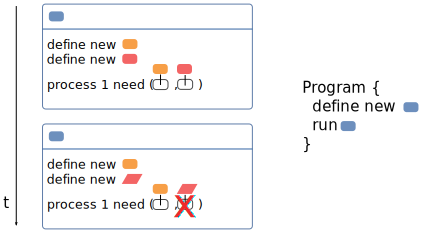
\includegraphics[width=.7\linewidth]{composants_principes_a.pdf}
  	\label{subfig_decouplage:a}}\qquad
  \subbottom[]{
	
\includegraphics[width=.8\linewidth]{composants_principes_c.pdf}
  	\label{subfig_decouplage:b}}
  \subbottom[]{
	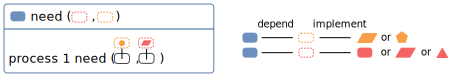
\includegraphics[width=.8\linewidth]{composants_principes_d.pdf}
  	\label{subfig_decouplage:c}}
 \end{sidecaption}
\end{figure}

Si on recontextualise ces principes à notre problématique, les classes de composants nécessaires à l'exécution minimale d'un algorithme évolutionnaire dans MGO sont décrites dans la figure \ref{fig:cake_classe}, et s'appuie sur le travail déjà décrit de la communauté des EA pour unifier la description de ces algorithmes.

\begin{figure}[!htbp]
	\begin{sidecaption}[fortoc]{Classe de composants nécessaires pour l'exécution d'un EA.}[fig:cake_classe]
		\centering
		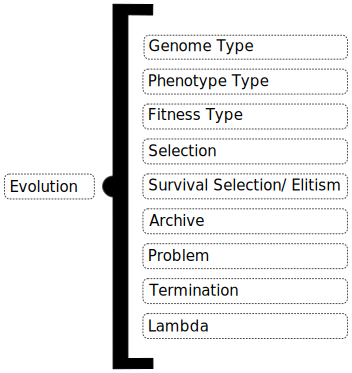
\includegraphics[width=0.7\linewidth]{cake_example.pdf}{
		}
  \end{sidecaption}
\end{figure}

Chacune de ces classes de composants est définie comme nécessaire pour le fonctionnement d'un algorithme d'évolution, dont la mise en dynamique du comportement générique est implémentée dans le composant \keyword{Evolution}. Tant que l'utilisateur n'aura pas fourni un composant compatible avec chacun de ces types de composants, alors le composant \keyword{Evolution} ne pourra pas s'exécuter. Le programme est défini comme un texte à trou, les boites sont bien placées, et le programme prêt à être exécuté suivant cet ordre, seulement ce n'est qu'un patron, une image, et cet ensemble de boites dont seule une partie de la logique a été intégrée, doit encore être complété par l'utilisateur. C'est un peu comme un puzzle dans lequel il manque des pièces, vous devez soit créer de nouvelles pièces, soit retrouver les pièces qui respectent la forme de chaque emplacement pour que le puzzle soit de nouveau complet.

L'inversion de contrôle détaillée dans les paragraphes précédents se matérialise de nouveau ici au travers du fait que c'est l'utilisateur qui définit sa composition, en s'assurant avec l'aide des instructions du programme que les dépendances propres au fonctionnement de chacun des composants sont bien fournies. Tout programme ne remplissant pas les conditions renverra un message d'erreur à son execution. En ce sens MGO est probablement plus un \textit{framework} qu'une librairie logicielle \Anote{martin_fowler}. L'autre avantage d'une telle approche c'est que l'application peut être livrée avec un vaste catalogue de pièces compatible avec chaque type d'emplacement, laissant à l'utilisateur la possibilité de choisir sa propre combinaison, voire même de créer ses propres pièces s'il estime quelles sont manquantes.

Ils existent différentes techniques pour qu'une telle architecture puisse être mise en oeuvre. Par exemple l'utilisation mixte de \textit{classe abstraite} et d'\textit{interfaces} permettent dans de nombreux langage informatique, comme Java ou C\#, de reproduire le découplage entre composants tel qu'on la vu dans la figure \ref{fig:decouplage_principe}.

En réalité, pour certains programmeurs \textcite{Odersky2005} \Anote{odersky_note_cake} ce type de techniques, dont l'existence, les avantages et les contraintes ont largement été discutés, ne constitue pas selon lui la meilleure réponse d'un point de vue technique pour garantir une meilleure réutilisabilité des composants informatiques. Il faut savoir à ce sujet qu'il existe en informatique une branche de recherche tourné vers la construction de langage de programmation aux caractéristiques innovantes. Ainsi les propriétés du langage Scala utilisé pour implémenter MGO expose la solution fournie par Martin Odersky à cette question de recherche que représente la recherche d'une meilleure modularité des programmes informatiques. Tout comme dans les années 1980, le langage Smalltalk d'Alan Kay a introduit une autre façon de structurer les programmes avec le paradigme Orienté Objet, Scala permet ici de penser de façon originale la modularité des composants en usant d'un tout nouveau couplage de différentes abstractions informatiques ( \textit{abstract type members}, \textit{explicit self-types}, \textit{modular mixin composition}) \Anote{note_informatique_mixin}. Autrement dit, ce que Scala va nous permettre d'exprimer comme degré de modularité lors de la description informatique de nos composants constitue en soit une innovation qui n'est pas présente, ou présente sous des formes trop complexe vis à vis de notre cahier des charges, dans bien d'autres langages informatiques.

%Si l'utilisation de classe abstraite est donc intéressante, elle ne résout pas tout les problèmes à elle seule. Ainsi par exemple, lorsqu'on utilise des classes abstraites, il n'est pas possible d'utiliser des dépendances cycliques entre composants, et la nécessité de respecter un ordre d'initialisation entre composants devient également rapidement une contrainte.

%Scala permet par exemple de définir des \keyword{traits} qui possède des caractéristiques plus intéressant que des classes abstraites ou des interfaces, tout en assurant à minima un comportement similaire. Il est par exemple possible d'assembler, de mixer de façon dynamique plusieurs traits, et l'addition des comportements se fait automatiquement.

%Il est également possible de définir des traits qui contiennent totalité ou seulement partie d'une implémentation. Ce type de programmation n'est pas permises par d'autres langage informatique, comme Java par exemple.

Souvent apellé de façon jargonnesque \foreignquote{english}{Cake Pattern} pour la possibilité de composition qu'elles offrent (comme dans un cake, un gateau dont la recette peut accueillir une très grande variété d'étapes, de composantes), ces outils aussi connus sous le nom \foreignquote{english}{Scalable Component Abstractions} ou encore \foreignquote{english}{Component Based Dependency Injection} regroupent  l'ensemble des techniques permettant d'accéder à cette modularité est donc présente de façon native dans le langage, car pensé et implémenté par son créateur \autocite{Oderskyxx}.


La figure \ref{fig:principe_mixin} expose les différentes

\begin{figure}[!htbp]
	\begin{sidecaption}[fortoc]{Un exemple plus proche de l'implémentation, appuyé par une version UML orienté Scala, pour comprendre comment les élements manquants (attributs, méthodes) définis en \sqbox{tangoRed1} dans ce diagramme de classe sont indiqués au programme lors de la création de nouveau objets. Les boites rouges représentent les erreurs retournés à l'utilisateur lors des tentatives successives de déclaration d'un nouvel élément \keywordmin{D1}, puis \keywordmin{D2}. \parbox{\marginparwidth}{
\begin{enumerate}[label=(\alph*),labelindent=\parindent,leftmargin=*]
       \item Un diagramme UML pour illustrer un scénario de dépendance entre trois composants exemples \keywordmin{A}, \keywordmin{B}, et \keywordmin{C}. Le composant A utilise une fonction run qui nécessite la définition d'une \keywordmin{methode\_b} et d'une \keywordmin{methode\_c} provenant d'un composant de type \keywordmin{B} et \keywordmin{C}.
       \item Un premier scenario illustre de façon simplifié la logique d'héritage permettant la création d'un nouveau composant D1 à partir des composants A, B1 et C1.
       \item Dans ce deuxième scénario, on illustre la nécessité de rédéfinir dans D2 les attributs, mais également les méthodes, qui n'ont pas été apporté par des composants extérieurs.
\end{enumerate}}}[fig:principe_mixin]
	\centering
	\subbottom[]{
		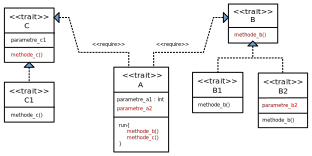
\includegraphics[width=0.8\linewidth]{exemple_mixin.pdf}
		\label{subfig_principe_mixin_a}}
	\subbottom[]{
		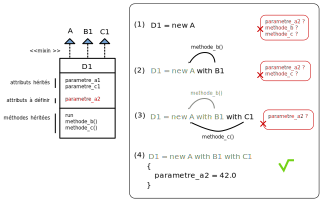
\includegraphics[width=0.8\linewidth]{exemple_mixin2.pdf}
		\label{subfig_principe_mixin_b}}
	\subbottom[]{
		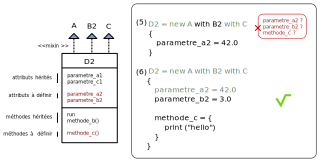
\includegraphics[width=0.8\linewidth]{exemple_mixin3.pdf}
		\label{subfig_principe_mixin_c}}
	\end{sidecaption}
\end{figure}

%Utilisé de façon complémentaire ces deux techniques permettent une grande flexibilité, une méthode ou un attribut est définit comme abstrait, et son implémentation doit être apportée par un composant externe.

%utilisant le cake pattern ( abstract type members, explicit self-types, modular mixin composition )

\subsubsection{Mobiliser les bons composants}

Un des grand défaut de cette technique, c'est qu'elle rend souvent la lecture du code source plus difficile du point de vue d'un observateur extérieur. Le programme est en effet morcelé dans un ensemble de composants contenant chacun une petite partie de la logique du programme total, assemblé par le compilateur avant l'execution du programme. De plus lorsque l'utilisateur choisit un composant, celui-ci ne fait pas qu'offrir de nouvelles alternatives à l'utilisateur, il en retire également, comme on pourrait s'attendre lorsqu'on manipule un arbre de dépendance complexe.

\hl{legende a faire, probleme entre les deux exemples.}

\begin{figure}[!htbp]
	\begin{sidecaption}[fortoc]{Illustration d'un premier scénario dans la selection de composant parmis les types $X$, et $Z$}[fig:composant_expli1]
		\centering
		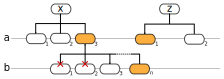
\includegraphics[width=0.7\linewidth]{dependanceExemple.pdf}{
		}
  \end{sidecaption}
\end{figure}

Si on considère un programme simplifié ayant besoin de deux types de composants pour fonctionner : $X$ et $Z$. Dans le premier scenario \ref{fig:composant_expli1}, l'utilisateur à choisi le composant $Z(a1)$ autonome, ainsi que le composant $X(a3)$. Ce dernier, contrairement au composant $X(a1)$ et $X(a2)$, dépend de nouveaux composant définis sur la ligne $b$ du schéma. On voit que dans les nombreux composants disponibles dans cette catégorie, seuls quelque uns s'avérent compatible avec le reste de la configuration de composant choisi par l'utilisateur. Que se passe t il lorsque l'utilisateur choisi pour $Z$ le deuxième composant $Z(2a)$ ?

\begin{figure}[!htbp]
	\begin{sidecaption}[fortoc]{Illustration d'un deuxième scénario dans la selection de composant parmis les types $X$, et $Z$.}[fig:composant_expli2]
		\centering
		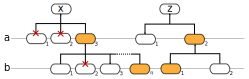
\includegraphics[width=0.7\linewidth]{dependanceExemple2.pdf}{
		}
  \end{sidecaption}
\end{figure}

C'est ce scénario qui est développé dans l'exemple \ref{fig:composant_expli2}. On voit que le choix de $Z(2a)$ implique de nouvelles restriction de choix dans la branche $X$, mais aussi la possibilité de nouveaux choix. Ainsi $X(b2)$ qui n'était pas compatible avec le composant $Z(a1)$ devient compatible avec au moins un des composants de $Z$, à savoir ici le composant $Z(b1)$ dont dépend $Z(a2)$ selectionné par l'utilisateur.

%Prenons un exemple simple, si l'utilisateur décide de ne pas utiliser de composant pour l'\keyword{Archive} des meilleurs individus, alors c'est tout un ensemble de stratégies dépendant de l'existence de ce composant dans le programme qui ne peux plus être mobilisé.

\subsubsection{Définition d'une méta-heuristique dans MGO}

L'implémentation d'un algorithme méta-heuristique prend cette forme dans MGO :

\begin{listing}[H]

\begin{minted}[linenos=true,frame=single,fontsize=\footnotesize]{scala}

trait NSGAII <: Evolution
  with BinaryTournamentSelection
  with TournamentOnRankAndDiversity
  with NonDominatedSorting
  with SBXCrossover
  with PolynomialGAMutation
  with GAGenome
  with Crowding
  with Pareto
  with NonStrictDominance
  with NoArchive
  with GeneticBreeding
  with MGFitness

\end{minted}
\caption{Exemple de définition d'une méta-heuristique dans MGO}
\label{alg:nsga2}
\end{listing}

La structure interne des composants constitutif de l'algorithme NSGA2 est lisible dès lors qu'on a déjà étudié le fonctionnement de métaheuristique. Chacune des briques (ici une par ligne) peut être remplacé ou modifié à partir du moment ou les conditions de dépendance entre composants sont respectés.

\begin{figure}[!htbp]
	\begin{sidecaption}[fortoc]{Schéma de dépendance existant entre les différents types de composants pour la définition de l'algorithme NSGA2 sous MGO}[fig:cake_classe]
		\centering
		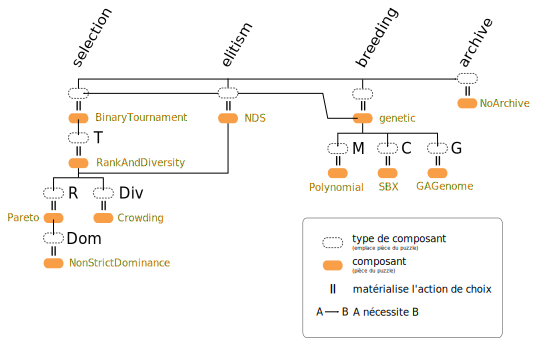
\includegraphics[width=0.9\linewidth]{diagrammeclassemgo.pdf}{
		}
  \end{sidecaption}
\end{figure}

Avoir accès de façon lisible permet de mieux comprendre les différences entres les différents algorithmes. Prenons un exemple simple de construction d'algorithme génétique multi-objectif utilisant l'algorithme de classement de solution candidates dites du \textit{Non Dominated Sorting} (NDS), tiré de \autocite{Goldberg1989} et implémenté par Deb dans NSGA \autocite{Deb1994} puis NSGA2 \autocite{Deb2001}. Pour fonctionner dans ces deux variantes, élitistes ou non élitistes, ce composant à besoin que l'utilisateur choisisse deux autres composants de type \keyword{Ranking}, et de type \keyword{Diversity}. Dans sa version non elitiste, le composant \keyword{Diversity} n'est pas utilisé.

Dans cet algorithme, les individus $x$ de la population $p_1$ sont partitioné selon un premier critère $c_1$, et de l'ensemble de partition ainsi formé, on ne retient que là premiere pour former un front $f$. Les individus de ce front sont supprimé de la population $p$, puis on recommence cette opération $n$ fois, cela jusqu'à ce que la somme des individus contenu dans l'ensemble des fronts $f_n$ soit égale à la population attendue pour $p_2$. Dans une utilisation non élitiste de cet algorithme, comme dans NSGA, la population $p_1 = p_2$. Dans une version élitiste, comme celle de NSGA2, la population $p_1$ contient également la progéniture (offspring), donc $p_2 = p_1 / 2$. Comme tout les individus de $p_1$ ne pourront pas participer à $p_2$, l'inclusion du dernier front dans $p_2$ doit être géré comme un cas particulier, et nécessite potentiellement d'être tronqué de façon intelligente, pour éviter de perdre en diversité. On fait donc appel à une méthode supplémentaire de calcul de diversité qui constitue en soit un deuxième critère de selection $c_2$ définissant les individus les uns par rapport aux autres.

Le choix d'un composant \keyword{Ranking} va déterminer quel va être le critère $c_1$ utilisé, et le choix d'un composant \keyword{Diversity} va déterminer selon quel critère $c_2$ les individus participant au dernier front vont être selectionnés.

On voit bien que les stratégies permettant de fixer ces deux critères peuvent être de nature très différentes. Pour $c_1$ le critère permettant de créer les ensembles le plus classique est le critère de dominance de Pareto définit par le composant du même nom \keyword{ParetoRanking}, mais d'autres critères sont tout à fait envisageable.

\hl{ A corriger avec les evolutions proposés}
Inversement, la même brique atomique définissant le calcul de dominance de Pareto est ainsi utilisé pour différents algorithmes canoniques, comme MOGA ou bien NSGA2. Ainsi là ou NSGA va utiliser cette brique plusieurs fois dans le composant NDS, MOGA va utiliser ce composant une seule fois en l'encapsulant dans un autre composant qui implémente la façon dont MOGA partitionne les individus.

Pour $c_2$, le critère utilisé par NSGA2 est une distance de crowding, mais là aussi d'autres variantes existe, comme par exemple le calcul d'hypervolume de Ziztler, Baume.

Le défaut majeur d'une telle approche, c'est qu'elle ne renseigne immédiatemment l'expérimentateur sur les choix valides ou invalides qui sont à sa disposition, et celui-ci peut alors se perdre dans une logique d'execution du code très éclaté. Pour résoudre ce problème, deux stratégies sont mise en oeuvre, la première c'est celle que l'on observe dans le listing \ref{alg:nsga2}, à savoir l'implémentation pré-existante dans le framework de plusieurs algorithmes évolutionnaires canonique prêt à l'emploi, et donc également prêt à être modifié, comme CMAES \autocite{Hansen}, NSGA2 \autocite{Deb2001}, ou SMS-EMOA \autocite{Beume2007}.

\hl{Capture d'écran à faire avec Mathieu L.}

%%JANET est en cours.

Un outil est également en cours de développement par Mathieu Leclaire pour explorer ce type de graphe. Nommé \textit{JANET}, cette application est capable de lire et de reconstruire le graphe de dépendance entre les différents composants d'un programme qu'on lui donne à explorer. A partir de là, il autorise l'experimentateur à composer son propre graphe de façon totalement interactive, en cliquant sur les composants du graphe.

A chaque selection de composant dans le graphe, l'ensemble des dépendances est recalculé afin de montrer à l'utilisateur quelle dépendance sont accessible de façon valide à partir de ses choix. Enfin \textit{JANET} est capable de générer un squelette de code similaire à celui exprimé dans le listing \ref{alg:nsga2}, utilisable directement comme nouvel algorithme.

\subsubsection{Définition d'un problème d'optimisation}

\hl{a finir peut etre avec un exemple concret de définition d'algorithme génétique usant d'une fonction test.}

\begin{listing}[!htbp]

\begin{minted}[linenos=true,frame=single,fontsize=\footnotesize]{scala}

trait Schaffer extends GAProblem with MGFitness {

  def genomeSize = 1
  def min = Seq.fill(genomeSize)(-100000.0)
  def max = Seq.fill(genomeSize)(100000.0)

  type P = Seq[Double]

  override def express(g: Seq[Double], rng: Random) = Seq(f1(g(0)), f2(g(0)))
  override def evaluate(p: P, rng: Random) = p

  def f1(x: Double) = pow(x, 2)
  def f2(x: Double) = pow(x - 2, 2)

}

\end{minted}
\caption{Exemple de définition d'un problème multi-objectifs dans MGO}
\label{alg:Schaffer}
\end{listing}

La librairie est conçu de façon à être totalement indépendante, car elle intègre à la fois les concepts nécessaire à la définition du problème, et la résolution d'un problème. En ce sens, elle peut donc être utilisé ou intégré à n'importe quel autre logiciel qui respecte le formalisme mis en place.

Le listing \ref{alg:Schaffer} est un exemple de définition d'un problème d'optimisation dans MGO. Dans celui-ci, il s'agit de résoudre la fonction test F2 multi-objectif de Schaffer \textcite[94]{Schaffer1985}, déjà définit dans l'équation \ref{eq:schaffer}.

La ligne 5 contient la signature du composant, et indique à MGO qu'il s'agit d'un problème de type algorithmes génétique \keyword{GAProblem} de type multi-objectif \keyword{MGFitness}.

Pour que le composant \keyword{GAProblem} soit opérationel, celui-ci a besoin que l'utilisateur lui fournisse un certain nombre d'élements en entrée : une taille de génome \keyword{genomeSize}, une type de Phenotype \keyword{P}, la définition des fonctions \keyword{express(...)} et \keyword{evaluate(...)}.

\begin{figure}[ht]
	\begin{sidecaption}[fortoc]{Hierarchie entre les composants pour la définition d'un problème, un exemple avec la fonction de test F2 de Schaffer}[fig:hierarchieComposants]
	 \centering
	 	
\includegraphics[width=.7\linewidth]{HierarchieComposants.pdf}
	\end{sidecaption}
\end{figure}

Si on regarde les dépendances de \keyword{GAProblem}, alors on voit qu'il dépend de \keyword{Problem}, lui même étant défini comme étant une extension d'\keyword{Evolution}. Concrétement cela veut dire que le problème Schaffer ne pourra être résolu que si l'ensemble des composantes cumulées de \keyword{GAProblem} , \keyword{Problem} et \keyword{Evolution} sont satisfaites au moment de la résolution, défini dans la section ci dessous.

Les fonctions $f1$ et $f2$ prennent un seul et même paramètre de variation $x$ non contraint. La taille \keyword{genomeSize} du génome est donc fixé à 1, et la définition \keyword{min} et \keyword{max} de sa variation est fixé ici à $-10^{5}$ et $10^{5}$.

Le type \emph{P} indique la nature du phénotype attendu pour ce problème. Dans notre cas la représentation d'une solution candidate dans l'espace de solution $\mathbb{X}$ correspond à un vecteur de réels \emph{Seq[Double]} qui accueille le résultat des fonctions objectifs $f1$ et $f2$.

Les deux fonctions \keyword{express(...)} et \keyword{evaluate(...)} doivent également être définies car elles sont utilisés par le composant \keyword{Evolution}, et fixe les règles de constitution d'un \keyword{Individu}, une structure de données permettant de regrouper le génome, le résultat des fonctions objectifs pour ce genome, ainsi que le résultat de la future fitness.

\begin{itemize}[label=\textbullet, noitemsep, topsep=0pt, parsep=0pt, partopsep=0pt]
\litem{\keyword{express}} prend en paramètre un vecteur de double qui correspond à la taille du génome. Dans le cas de Schaffer, il n'y a qu'un seul paramètre $x$, donc le génome $g$ est de taille 1, et donc $g(0)$ correspond forcément à la seule valeur $x$ contenu dans le génome. Cette fonction retourne l'expression de la fonction objective à évaluer, donc un vecteur contenant l'expression des deux fonctions objectives $f1$ et $f2$.

\litem{\keyword{evaluate}} est une fonction qui prend un phénotype et renvoie un vecteur de valeur correspondant à l'évaluation des fonctions objectifs. Ici les valeurs de $f1$ et $f2$

\end{itemize}

Dans le cas d'une simulation, \keyword{express} est la fonction qui va exécuter le modèle de simulation et récupèrer les valeurs en sortie, qui constitue le Phénotype. On voit bien ici que le phénotype ne permet pas forcément de discriminer les résultats de deux simulations, autant il peut s'agir d'indicateur réutilisable directement comme fonction objectifs, autant il peut également s'agir de données brutes qui peuvent être analysé en de multiples façons.  La fonction \keyword{evaluate} applique le vecteur de fonctions objectifs sur ces mesures en sortie de simulation. Un \keyword{Individu} dans la \keyword{Population} est une structure de données composée d'un Genome (paramètres du modèles), du résultat de la fonction \keyword{express} qui transforme un Génome en Phénotype, et du résultat de la fonction \keyword{evaluate} qui transforme un Phenotype en vecteur de valeurs d'objectifs.

%difference par rapport aux autres librairies ?

\paragraph{Execution d'un problème d'optimisation}

\begin{listing}[H]

\begin{minted}[linenos=true,frame=single,fontsize=\footnotesize]{scala}

object TestNSGAII extends App {

  val resolve =
    new Schaffer with NSGAII with CounterTermination {
      def steps = 1000
      def mu = 200
      def lambda = 200
      def genomeSize = 1
    }

  implicit val rng = newRNG(42)

  val res =
    resolve.evolve.untilConverged {
      s => println(s.generation)
    }
}

\end{minted}
\caption{Evaluation d'un problème multi-objectif à l'aide de l'algorithme NSGA2}
\label{alg:Evaluation_Schaffer}
\end{listing}

Dans l'implémentation \ref{alg:Evaluation_Schaffer}, la variable \keyword{resolve}  contient la définition de la marche à suivre : il s'agit ici de résoudre le problème \keyword{Schaffer} (voir \ref{alg:Schaffer}) en utilisant la métaheuristique \keyword{NSGA2} (voir \ref{alg:nsga2}) en utilisant un indicateur de fin d'optimisation de type compteur de génération \keyword{CounterTermination}.

\hl{verifier mu et lambda dans le code MGO}
Les variables \keyword{steps} (nombre d'itération avant arrêt de la métaheuristique), \keyword{mu} (), \keyword{lambda} (), \keyword{genomeSize} (taille du génome) sont des variables qui n'ont pas trouvé de valeur dans la composition du graphe de dépendance reliant les différents composants, le compilateur fait donc remonter (sous forme d'erreur à la compilation) la nécessité de définir ces variables aux derniers niveau de définition, qui constitue la tête de l'arbre, afin que ceux ci soient renseignés par l'utilisateur.


\subsubsection{La mise en oeuvre du couplage MGO - openMOLE }

Dans la section justifiant la création d'une nouveau framework dédié aux méta-heuristiques, on a abordé des points d'objectifs à la fois centré sur les capacités finale de MGO en tant que framework flexible, extensible, autonome; mais également sur les capacités tout autres attendues pour une utilisation de ce framework dans un outil spécialisé dans la distribution transparente des calculs, openMOLE.

Concevoir des logiciels capable de s'exectuer sur des environnement distribués est une spécialité informatique en tant que telle, usant de technologie et de jargon déjà difficile d'accès à des développeurs spécialisé, et donc encore moins accessible à un public plus interdisciplinaire comme les chercheurs en SHS.

Il n'est donc pas question d'associer, du moins dans un premier temps, une myriade d'interface au framework MGO à destination d'un couplage direct avec les technologies \textit{HPC} ou de \textit{Grid Computing}. Il me semble être beaucoup plus intéressant de ne pas complexifier outre mesure la librairie MGO, et de profiter du fait qu'il s'agit d'un \textit{framework} pour composer des métaheuristiques plus adaptés à l'usage maximum qui peut être fait des ressources disponibles. En soit, MGO peut dans sa version autonome satisfaire un public scientifique exigeant sur le volet d'une recherche théorique dans le domaine des méta-heuristiques, tout en proposant dans un plugin pour openMOLE, des métaheuristiques adaptés à un tout autre public, attiré par l'efficience de ces algorithmes pour des cas d'utilisation très spécifique qui n'ont que très peu avoir avec les \textit{benchmarks} que l'ont trouve par exemple dans la littérature des EA. Dans cette configuration, composer ces propres métaheuristiques reste toujours possible, mais demande un peu plus de connaissance technique pour modifier le code du plugin faisant l'interface entre MGO et openMOLE. Le tableau \ref{tab:resume_public_cible} aborde de façon synthétique ces deux points de vue utilisateurs par rapport aux principales qualités attendues du programme : Flexibilité, Extensibilité, Utilisabilité.

% http://www.tablesgenerator.com/latex_tables#
% Ajouter une couleur sur la partie +++ a mettre en valeur coté plugin MGO

\begin{table}[!htbp]
\begin{sidecaption}[fortoc]{Résumé des avantages et des inconvénients à atteindre selon le public cible. \parbox{\marginparwidth}{
\begin{enumerate}[label={},noitemsep,  parsep=0pt, partopsep=0pt, labelindent=0pt,leftmargin=*]
		\item $-$ assez difficile
		\item $-{}-$ difficile
		\item $-{}-{}-$ très difficile
		\item $+$ assez facile
		\item $++$ facile
		\item $+++$ très facile
\end{enumerate}}}
	[tab:resume_public_cible]
	\centering
	\begin{tabular}{llllll}
		\toprule
		\multicolumn{2}{l}{\multirow{2}{*}{}} & \multicolumn{2}{l}{modélisateur} & \multicolumn{2}{l}{informaticien} \\ \cline{3-6}
		\multicolumn{2}{l}{} & Plugin Mgo & Mgo & Plugin Mgo & Mgo \\
		\midrule
		(1) & Flexible & $-{}-$ & $+$ & $+$ & $+++$ \\
		(2) & Extensible & $-{}-{}-$ & $-$ & $+$ & $++$ \\
		(3) & Utilisable & $+++$ & $+$ & $+++$ & $+++$ \\
		\bottomrule
		\end{tabular}
  \end{sidecaption}
\end{table}

\begin{enumerate}[label=(\arabic*)]
\item Du point de vue de la flexibilité des métaheuristiques proposés, c'est-à-dire de la possibilité de combinaisons de composants offertes par MGO, elle est censé être identique que cela soit dans le plugin ou directement avec MGO. Toutefois, cette flexibilité est beaucoup plus difficile à mettre en oeuvre dans le plugin pour des non informaticiens, car la logique d'exécution des métaheuristiques est éclatée dans différentes tâches d'un workflow openmole afin que certaines d'entre elles soient parallélisés (voir la section suivante \ref{p:prototype_fonctionel}). De nouveaux algorithmes métaheuristiques spécialisés pour une utilisation sur grille de calcul font également leur apparition dans le plugin, et constitue des worflow beaucoup plus complexes, assez difficilement accessibles à la modification par des modélisateurs géographes.

\item Ajouter ou modifier de nouveaux algorithmes dans le plugin openMOLE nécessite de maitriser sufisament bien à la fois l'ensemble du vocabulaire (aussi apellé \textit{Domain Specific Language} DSL openMOLE) nécessaire pour définir des workflows, mais également le langage de programmation Scala qui dans le plugin est mélé de façon beaucoup plus complexe à ce vocabulaire. Une fois ces premières connaissances acquise, et avant même de pouvoir créer de nouvelles méta-heuristiques, il faudra comprendre en observant les métaheuristiques déjà implémenté comment d'une part les composants MGO sont encapsulés et chainés dans un workflow complexe mélant Scala et le DSL openMOLE, et d'autre part comment ce workflow voit sa complexité encapsulé dans un élément de vocabulaire nouveau accessible directement au niveau du DSL. Si ce travail peut effectivement être réalisé sans trop de difficulté par un informaticien un peu expérimenté, l'exercice paraitra très difficile voire hors de portée à un modélisateur géographe.

\item L'utilisation du plugin dans openMOLE doit être rendu le plus simple possible pour le modélisateur et l'informaticien. En revanche l'utilisation du framework de façon autonome demande pour un modélisateur quelque compétences techniques supplémentaires pour installer les logiciels adéquats permettant de modifier et compiler MGO. Une fois cette barrière technique dépassé, la connaissance du langage Java ou Scala est certe nécessaire pour modifier ou ajouter des composants, mais elle ne l'est pas forcément lorsqu'il s'agit d'imbriquer et de paramétrer les composants correctement.

\end{enumerate}

Si le framework MGO est parfaitement utilisable de façon autonome, celui-ci ne bénéficie pas dans ce mode d'utilisation des algorithmes dédiés pour une utilisation sur des environnements distribués.

Or c'est bien cette utilisation que nous voulons rendre disponible aux modélisateurs, à la différence des librairies intégrés existantes, comme par exemple \textit{behaviorSearch} que l'on a déjà décrit dans la \ref{section xx}.


La mise à disposition de ce framework dans le cadre d'un plugin pour openMOLE fait intervenir de tout nouveaux objectifs, cette fois ci relatifs aux intéréts des modélisateurs.

En effet, si les métaheuristiques se doivent effectivement d'être modifiable, ce n'est pas forcément cet aspect qui prime pour une utilisation dans la modélisation; qui subit une fois la base du modèle réalisé des cycles de développements assez courts en définitive, ceux ci se limitant la plupart du temps à des ajouts, des modifications, ou des retraits d'hypothèse. L'utilisation de méta-heuristique, même canonique, est un premier palier d'utilisation pour tenter de discriminer au plus vite les modèles de simulation. Dans ce cas c'est bien les propriétés d'efficacité et d'indépendance au problème que l'on mobilise dans l'utilisation de métaheuristique. La modification plus fine est un cas d'utilisation qui vise une adaptation spécifique de la réponse d'une métaheuristique à un problème, ce qui nécessite de la part de celui-ci une variabilité moindre que dans le cas d'un construction de modèle.


On a vu précédemment que la recherche d'une architecture logicielle modulaire était avant tout guidé par la nature elle même très modulaire des métaheuristique.



L'histoire MGO tel qu'avancé dans la section \ref{ssec:historique_mgo}, un autre objectif à guider la réalisation d'un framework aussi modulaire.

% evaluate et express sont dans la meme tache dans OpenMOLE

\subsection{Premiere prototype fonctionel}
\label{p:prototype_fonctionel}

La constitution d'un premier prototype fonctionnel constitue pour l'équipe un triple retour d'expérience, pour MGO, pour openMOLE, et évidemment pour le modèle utilisé, à savoir Simpop Local.

Avant mars 2012, le couplage entre MGO et openMOLE est réalisé par l'utilisateur lors de la définition des workflows. Grâce à la nature autonome et modulaire des composantes fournies par l'univers du framework MGO, la logique d'execution d'une métaheuristique peut facilement être retranscrite dans le référentiel d'openMOLE. Les tâches d'un workflow vont tout simplement encapsuler les appels et les objets spécifiques aux différentes composantes de la métaheuristique, en apportant la logique nécessaire à une execution de certaines de ces composantes dans un environnement de calcul distribué.

Autrement dit, la logique d'execution générique d'une métaheuristique décrite dans la composante \keyword{Evolution} est instancié (par exemple on choisit d'implémenter NSGA2) puis éclaté dans un ensemble de tâches dont l'organisation est guidé à la fois par la reproduction de cette optimisation, mais aussi par la parallélisation de certaines de ces tâches.

Un tel workflow doit également s'aclimater de toute la logique d'experimentation pour un modèle de simulation. Des tâches intermédiaires font donc leur apparition dans le workflow pour gérer un plan d'expérience particulier.

La nature intrinsèquement parallèle des algorithmes evolutionnaires tient dans la possibilité d'évaluer non pas les solutions candidates une par une, mais bien d'un seul coup, par l'évaluation de l'ensemble des solutions candidates d'une population à un instant $t$. La première étape a donc été de distribuer l'évaluation des solutions candidates sur un environnement distribué, afin de bénéficier d'une execution quasi simultanée de l'ensemble de la population.

\begin{figure}[H]
	\begin{sidecaption}[fortoc]{wf openmole \sqbox{tangoBlue1}}[fig:openmole_wf]
		\centering
		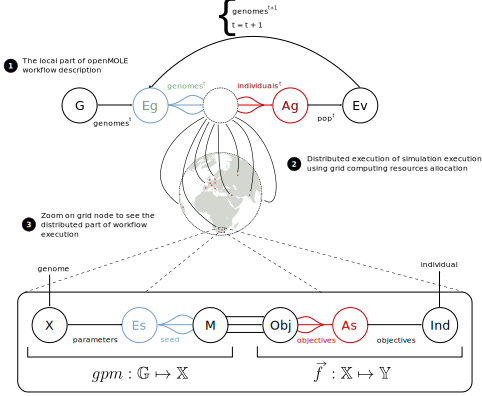
\includegraphics[width=1.1\linewidth]{wf_openmole_mgo_1.pdf}{
		}
  \end{sidecaption}
\end{figure}

On considère les paramètres suivant, une population initiale de génomes $n$, et le nombre de réplication à exécuter pour chacun de ces génomes équivalent à $r$; Autrement dit, à chaque itération $t$ de l'algorithme d'optimisation, c'est $n$ jeu de valeur de paramètres différentes (équivalent génome) qui vont chacune être testé $r$ fois avec des graines aléatoires différentes. Soit un total final de $n * r * t$ simulations.

Avant de rentrer dans les détails du workflow, il est également important de rapeller que dans celui-ci, un \keyword{Genome}, et par la suite un \keyword{Individu} dans une \keyword{Population}, sont deux dénominations qui désignent avant tout un jeu de valeur de paramètres, même si un individu représente on va le voir un peu plus que çà. Autrement dit, quant on discute ici de la qualité d'un \keyword{Individu} et de son positionnement dans l'espace des objectifs $\mathbb{Y}$, c'est sous entendu en référence au jeu de valeur de paramètre qui a permis d'obtenir ce même \keyword{Individu}.

Le premier niveau de workflow (étape \circled{1} dans la figure \ref{fig:openmole_wf}) opérant de façon locale sur la machine ou le serveur de l'utilisateur est décrit ainsi :

%\begin{itemize}[label=\textbullet]

\begin{myitemize}

\item[G] Cette tâche définit comment le problème va être représenté par le \keyword{Genome} durant l'optimisation. C'est aussi à ce moment là que le mapping est réalisé avec les paramètres du modèles, avec par défaut 1 gène par paramètre $p$ du modèle. Cette tâche génère ensuite un ensemble de génomes $g_i \in \{g\}, i \in \{1 \dotsc n\}$ chacun étant initialisé par des valeurs de paramètres aléatoires.

\item[Eg] Cette première tâche d'exploration exécute un plan d'expérience qui associe à chaque \keyword{Genome} $g_i$ une liste de graines aléatoires  - ou \textit{seeds} - $\{s_i\}$. Cette liste d'éléments $s_{i,r} , s_{i,r} \in \{s_i\}, r \in \{1 \dotsc r\}$ est de taille égale au nombre de réplications $r$ définies en paramètre de l'expérimentation. De ce plan d'expérience résulte la création d'un ensemble $\{w\}$ de sous workflows équivalent au nombre de génomes initial $n$. Chaque $w_i$ est organisé selon la description du deuxième niveau de workflow décrit ci-dessous, distribué de façon transparente sur un des noeud de la grille de calcul par openMOLE (étape \circled{2} dans la figure \ref{fig:openmole_wf}) avec pour paramètre d'entrée le vecteur $(g_i, \{s_i\})$.

\item[Ag] Chaque sous workflow $w_i$ s'executant sur grille renvoie un \keyword{Individu} évalué, une structure de donnée qui associe pour chaque \keyword{Genome} $g_i$, un \keyword{Phenotype} et un vecteur d'objectifs $f_i$. Cette tâche d'aggrégation collecte ces individus auprès de l'ensemble des sous workflow de façon à former un ensemble d'\keyword{Individu} formant une nouvelle \keyword{Population} $P$. Cette dernière est ensuite transmise pour examen à la tâche suivante \textit{Ev}.

\item[Ev] Cette tâche contient le coeur de l'algorithme d'optimisation, dont le comportement est fonction de l'algorithme évolutionnaire selectionné ou composé, et des paramètres choisi par l'utilisateur pour celui-ci. Dans une première phase, la population nouvellement constituée est fusionnée avec la population d'individu de la génération précédente. Une fitness est attribuée à chaque individu de cette nouvelle population, ce qui permet de caractériser la qualité de chacune de ces solutions dans l'espace des objectifs de façon relative à l'algorithme utilisé. S'ensuit alors une première phase élitiste de selection qui opère sur la base de ce score. Les individus selectionnés participent ensuite de nouveau à un tirage au sort pour tenter d'intégrer le pool d'individu (\textit{mating pool}) participant à la reproduction, étape durant laquelle emerge un ensemble de nouveaux génomes à évaluer, transmis à la tâche \textit{Ev} pour une nouvelle distribution.
\end{myitemize}

Le deuxième niveau de workflow (étape \circled{3} dans la figure \ref{fig:openmole_wf}), celui qui s'exécute sur un noeud distant de la grille de calcul, contient les tâches suivantes :

\begin{myitemize}

\item[X] Cette tâche extrait les valeurs de paramètre du génome $g_i$ qui est donné en entrée de ce sous workflow, et les transmets avec l'ensemble des $r$différentes \textit{seeds} de l'ensemble $\{s_i\}$ à une nouvelle tâche d'exploration \textit{Es}

\item[Es] définit un nouveau plan d'expérience pour exécuter l'ensemble des réplications $s_{i,r}$ sur ce noeud local de la grille. A chaque réplication du modèle de simulation est associé un jeu de valeur de paramètre tel qu'il a été extrait du génome $g_i$ (toujours identique donc), ainsi qu'une \textit{seed}, prise dans $s_{i,r}$ avec $r$ différent pour chaque réplication.

\item[M] exécute le modèle de simulation avec la graine aléatoire $s_{i,r}$ et le jeu de valeur de paramètre fourni. Cette étape est équivalente à la constitution du Phénotype.

\item[Obj] applique aux résultats de la simulation les fonctions objectifs définis par l'utilisateur dans le workflow

\item[As] récupère les vecteurs de valeurs objectifs associées à chaque réplication du modèle de simulation, et les aggrege selon une fonction statistique choisi par l'utilisateur, une moyenne ou une médiane par exemple.

\item[Ind] crée un \keyword{Individu}, une structure de donnée associant le \keyword{Genome} $g_i$ évalué et le vecteur objectifs précédemment agregé. La \textit{seed} n'est pas conservé dans cette expérience ou on recherche avant tout un comportement robuste à l'aléa.

\end{myitemize}

Les premiers workflows \Anote{cas_utilisation_wfom}, assez complexes et uniquement accessibles au format scripts, ont rapidement constituées des fichiers de plusieurs centaines de lignes. Cette évolution dans la taille des workflows est rapidement devenu problématique à la fois pour la maintenance mais également pour la lisibilité de tels expérimentations. Un obstacle vis à vis de notre principal objectif, mettre à disposition des modélisateurs un outil dont le premier avantage est sa facilité de mise en oeuvre et sa réutilisabilité.

Si l'exécution d'un tel workflow est déjà un premier pas vers une systématisation dans l'application de ces techniques d'optimisation à l'exploration des modèles de simulations, il faut soulever un autre point important aux yeux de l'utilisateur. Quelle performance peut on en effet attendre d'un tel workflow d'optimisation distribué lorsqu'il est appliqué sur un modèle de simulation relativement rapide en Netlogo ?

Si $n=200$, $r = 30$, $t=2000$, cela équivaut donc à 12 millions de simulations. Pour nous donner une durée d'execution, il faut encore multiplier par la durée d'exécution du modèle : un modèle jugé relativement rapide s'executant en moyenne en 2 minute sous Netlogo revient à cumuler environ 46 années de calcul sur un seul processeur. Sur une grille de calcul disposant de 1000 processeurs, cette durée descend à 17 jours. Sachant que de tels algorithmes évolutionnaire ne garantissent pas d'optimum global, ceux ci doivent également être répliqué afin de vérifier si l'algorithme, malgré notre vigilance sur les paramètres de celui-ci, ne serait pas malheureusement tombé dans un optimum local ?

Les premières explorations du modèle SimpopLocal ont été faites suivant ce workflow à partir d'avril 2011, mais c'est seulement en septembre 2011 que le couplage est présenté aux géographes à l'ECQTG d'Athènes, puis à des informaticiens à la conférence V2CS à Paris.

Il y a deux possibilités pour gagner en temps de calcul et permettre un retour d'expérience sur leur modèle plus rapide pour les modélisateurs. En effet, soit le modèle de simulation peut être optimisé, soit l'algorithme métaheuristique distribuant les simulations peut encore être amélioré. Seule la deuxième voie offre un gain de temps générique, quelque soit le modèle. Dans le cas de simpopLocal, la première voie a également été exploré, et le modèle écrit initialement en Netlogo, a d'abord accueilli un plugin en Scala pour externaliser les traitements les plus long, avant d'être finalement réécrit complétement en Scala.




- Amélioration de la rapidité d'exécution via application de nouvelle méthode de parallélisme des GA
- Amélioration dans la description des workflows


Un choix difficile s'offre au modélisateur voulant explorer de façon plus systématique

Quelles questions ?
- Comment effectuer une recherche plus exhaustive des comportements des modèles ?
- Comment discriminer les résultats d'un front de Pareto, quelle expertise humaine ?

Quels apprentissages ?
- Quels biais dans les modèles stochastique ?
- Nombre de réplications nécessaires, suffisantes ?
- Quel retour sur la thématique ?

Quelques pistes ?
- quels critères d'arrets ?
- quel espilon sur les objectifs ?
- quelle possibilité de réévaluation ?
- aller vers des algorithmes utilisant la grille de façon plus efficace
- réécrire les modèles
- réduire le nombre d'objectif
- réduire le nombre de réplication
- réduire la population d'individu
- réduire la durée de l'expérimentation
